%!TEX program = pdflatex
\documentclass{poly}
\title{Mathématiques~---~1\textsuperscript{ère} Générale (spécialité)}
\author{}
\date{\figureC{}}
% ----------------------------------------------------------------------------------------------------
\begin{document}
\maketitle
\tableofcontents
% ----------------------------------------------------------------------------------------------------
\part{Analyse}
\chapter{Fonctions du second degré}

La trajectoire d'un ballon, la forme d'une antenne parabolique ou l'aire d'un enclos : toutes ces situations se modélisent par une fonction du second degré.

Dans ce chapitre, on étudie les trois écritures d'un même trinôme, la résolution des équations et des inéquations associées, puis on les met au service de problèmes d'optimisation.

\section{Définition et différentes formes d'un trinôme}

\subsection{Forme développée}

\begin{df}
	On appelle \textbf{fonction polynôme du second degré} (ou \textbf{trinôme du second degré}) toute fonction $f$ définie sur $\R$ pouvant s'écrire sous la forme \textbf{développée} :
	\[
		f(x) = ax^2 + bx + c
	\]

	\ldots où $a$, $b$ et $c$ sont des nombres réels donnés, avec $a \neq 0$.
\end{df}

\begin{ex}
	\nline
	\begin{itemize}
		\item $f(x) = 2x^2 - 5x + 2$ est un trinôme du second degré, avec $a = 2$, $b = -5$ et $c = 2$.
		\item $g(x) = -x^2 + 4$ est un trinôme du second degré, avec $a = -1$, $b = 0$ et $c = 4$.
		\item $h(x) = (x-1)(3-2x)$ est un trinôme du second degré car en développant, on obtient :
		      \[
			      h(x) = -2x^2 + 5x - 3
		      \]

		      \ldots d'où $a = -2$, $b = 5$ et $c = -3$.
		\item $k(x) = (x+1)^2 - x^2$ n'est \emph{pas} un trinôme du second degré : en développant, on obtient $k(x) = 2x + 1$, qui est une fonction affine.
	\end{itemize}
\end{ex}

\begin{rem}
	La condition $a \neq 0$ est essentielle : si $a = 0$, la fonction $x \mapsto bx + c$ est affine.

	Par ailleurs, $f(0) = c$ : le nombre $c$ est l'ordonnée à l'origine de la courbe.
\end{rem}

\subsection{Forme canonique}

\begin{thm}
	Tout trinôme $f(x) = ax^2 + bx + c$ (avec $a \neq 0$) peut s'écrire, de manière unique, sous la forme \textbf{canonique} :
	\[
		f(x) = a(x - \alpha)^2 + \beta
		\qquad \text{avec} \qquad
		\alpha = \frac{-b}{2a} \quad \text{et} \quad \beta = f(\alpha)
	\]
\end{thm}

\newpage

\begin{demo}
	\nline
	\begin{itemize}
		\item \textbf{Existence.}

		      Comme $a \neq 0$, on factorise par $a$ :
		      \[
			      f(x) = a \left[ x^2 + \frac{b}{a}x + \frac{c}{a} \right]
		      \]

		      L'expression $x^2 + \dfrac{b}{a}x$ est le début du développement de $\left(x + \dfrac{b}{2a}\right)^2 = x^2 + \dfrac{b}{a}x + \dfrac{b^2}{4a^2}$.

		      Ainsi :
		      \[
			      x^2 + \frac{b}{a}x = \left(x + \frac{b}{2a}\right)^2 - \frac{b^2}{4a^2}
		      \]

		      En remplaçant dans l'expression de $f(x)$, il vient :
		      \[
			      f(x) = a \left[ \left(x + \frac{b}{2a}\right)^2 - \frac{b^2}{4a^2} + \frac{c}{a} \right]
			      = a \left[ \left(x + \frac{b}{2a}\right)^2 - \frac{b^2 - 4ac}{4a^2} \right]
		      \]

		      En distribuant le facteur $a$, on obtient :
		      \[
			      f(x) = a\left(x - \left(\frac{-b}{2a}\right)\right)^2 + \frac{4ac - b^2}{4a}
		      \]

		      On pose $\alpha = \dfrac{-b}{2a}$.

		      Pour $x = \alpha$, le terme $a(x-\alpha)^2$ s'annule, donc le dernier terme vaut bien $f(\alpha) = \beta$.

		\item \textbf{Unicité.}

		      Si $a(x-\alpha)^2 + \beta = a(x-\alpha')^2 + \beta'$ pour tout réel $x$, alors en développant et en identifiant les coefficients de $x$, on obtient $-2a\alpha = -2a\alpha'$, donc $\alpha = \alpha'$ car $a \neq 0$, puis $\beta = \beta'$.
	\end{itemize}
\end{demo}

\begin{methode}[Mettre un trinôme sous forme canonique]
	\nline
	\begin{enumerate}
		\item On identifie les coefficients $a$, $b$ et $c$.
		\item On calcule $\alpha = \dfrac{-b}{2a}$.
		\item On calcule $\beta = f(\alpha)$.
		\item On écrit $f(x) = a(x-\alpha)^2 + \beta$.
	\end{enumerate}
\end{methode}

\begin{ex}
	Soit $f(x) = 2x^2 - 8x + 3$.

	On a $a = 2$, $b = -8$ et $c = 3$, donc :
	\[
		\alpha = \frac{-\pa{-8}}{2 \times 2} = 2
		\qquad \text{et} \qquad
		\beta = f(2) = 2 \times 2^2 - 8 \times 2 + 3 = -5
	\]

	Ainsi $f(x) = 2(x-2)^2 - 5$.
\end{ex}

\begin{erreur}
	Dans la forme canonique, on écrit $(x - \alpha)^2$ :

	\begin{itemize}
		\item Si $\alpha = 2$, on écrit $(x-2)^2$ ;
		\item Si $\alpha = -3$, on écrit $(x+3)^2$.
	\end{itemize}

	Attention aussi au signe dans $\alpha = \dfrac{-b}{2a}$.
\end{erreur}

\subsection{Représentation graphique et variations}

La courbe représentative d'un trinôme du second degré est une \textbf{parabole}.

\begin{prop}
	Soit $f(x) = a(x-\alpha)^2 + \beta$ avec $a \neq 0$.
	\begin{itemize}
		\item La parabole possède un \textbf{sommet} $S\coordl{\alpha}{\beta}$.
		\item La droite d'équation $x = \alpha$ est un \textbf{axe de symétrie} de la parabole.
		\item Si $a > 0$, la parabole est \og tournée vers le haut\fg{} :
		      \begin{itemize}
			      \item $f$ est décroissante sur $\intof{-\infty}{\alpha}$, croissante sur $\intfo{\alpha}{+\infty}$,
			      \item $f$ admet un \textbf{minimum} égal à $\beta$, atteint en $x = \alpha$.
		      \end{itemize}
		\item Si $a < 0$, la parabole est \og tournée vers le bas\fg{} :

		      \begin{itemize}
			      \item $f$ est croissante sur $\intof{-\infty}{\alpha}$, décroissante sur $\intfo{\alpha}{+\infty}$,
			      \item et admet un \textbf{maximum} égal à $\beta$, atteint en $x = \alpha$.
		      \end{itemize}
	\end{itemize}
\end{prop}

\begin{center}
	\begin{minipage}[t]{0.48\linewidth}
		\centering
		\begin{tikzpicture}[scale=0.9]
			\draw[->] (-0.7,0) -- (3.9,0) node[right] {$x$};
			\draw[->] (0,-1.6) -- (0,2.8) node[above] {$y$};
			\draw[dashed, gris] (1.5,-1.4) -- (1.5,2.4) node[above] {\small $x=\alpha$};
			\draw[thick, bleu, domain=-0.2:3.2, samples=60, smooth] plot (\x, {0.8*(\x-1.5)^2-1});
			\draw[dashed, gris] (0,-1) -- (1.5,-1);
			\filldraw[rouge] (1.5,-1) circle (2pt) node[below right] {$S\coordl{\alpha}{\beta}$};
			\node[above right, rouge] at (1.5,0) {$\alpha$};
			\node[left, rouge] at (0,-1) {$\beta$};
		\end{tikzpicture}

		$a>0$ : minimum en $S$
	\end{minipage}\hfill
	\begin{minipage}[t]{0.48\linewidth}
		\centering
		\begin{tikzpicture}[scale=0.9]
			\draw[->] (-0.7,0) -- (3.9,0) node[right] {$x$};
			\draw[->] (0,-1.4) -- (0,2.4) node[above] {$y$};
			\draw[dashed, gris] (1.5,-1.2) node[below] {\small $x=\alpha$} -- (1.5,2.0);
			\draw[thick, bleu, domain=-0.2:3.2, samples=60, smooth] plot (\x, {-0.8*(\x-1.5)^2+1.5});
			\draw[dashed, gris] (0,1.5) -- (1.5,1.5);
			\filldraw[rouge] (1.5,1.5) circle (2pt) node[above right] {$S\coordl{\alpha}{\beta}$};
			\node[below right, rouge] at (1.5,0) {$\alpha$};
			\node[left, rouge] at (0,1.5) {$\beta$};
		\end{tikzpicture}

		$a<0$ : maximum en $S$
	\end{minipage}
\end{center}

\begin{prop}[Tableaux de variations]
	\nline
	\begin{center}
		\begin{minipage}[t]{0.48\linewidth}
			\centering
			$a>0$\par\ms
			\begin{tikzpicture}
				\tkzTabInit[lgt=1.5,espcl=2.2]{$x$/0.8,$f$/1.8}{$-\infty$,$\alpha$,$+\infty$}
				\tkzTabVar{+/$+\infty$,-/$\beta$,+/$+\infty$}
			\end{tikzpicture}
		\end{minipage}\hfill
		\begin{minipage}[t]{0.48\linewidth}
			\centering
			$a<0$\par\ms
			\begin{tikzpicture}
				\tkzTabInit[lgt=1.5,espcl=2.2]{$x$/0.8,$f$/1.8}{$-\infty$,$\alpha$,$+\infty$}
				\tkzTabVar{-/$-\infty$,+/$\beta$,-/$-\infty$}
			\end{tikzpicture}
		\end{minipage}
	\end{center}
\end{prop}

\begin{rem}
	Le coefficient $a$ commande aussi l'\og ouverture\fg{} de la parabole : plus $\abs{a}$ est grand, plus la parabole est resserrée autour de son axe de symétrie.

	\begin{center}
		\begin{minipage}[t]{0.48\linewidth}
			\centering
			\begin{tikzpicture}[>=Stealth]
				\begin{axis}[axis line style={thick}, width=\linewidth, height=5cm, axis lines=middle, xmin=-2.7, xmax=2.7, ymin=-0.5, ymax=5, xtick=\empty, ytick=\empty, legend columns=-1, legend style={at={(0.5,1.03)}, anchor=south}]
					\addplot[vert,  ultra thick, domain=-2.7:2.7, samples=60] {0.5*x^2};
					\addplot[dashed , bleu,  ultra thick, domain=-2.7:2.7, samples=60] {x^2};
					\addplot[dotted , rouge, ultra thick, domain=-2.7:2.7, samples=60] {2*x^2};
					\legend{$a=0.5\quad$, $a=1\quad$, $a=2$}
				\end{axis}
			\end{tikzpicture}
		\end{minipage}\hfill
		\begin{minipage}[t]{0.48\linewidth}
			\centering
			\begin{tikzpicture}[>=Stealth]
				\begin{axis}[axis line style={thick}, width=\linewidth, height=5cm, axis lines=middle, xmin=-2.7, xmax=2.7, ymin=-5, ymax=0.5, xtick=\empty, ytick=\empty, legend columns=-1, legend style={at={(0.5,1.03)}, anchor=south}]
					\addplot[vert,  ultra thick, domain=-2.7:2.7, samples=60] {-0.5*x^2};
					\addplot[dashed, bleu,  ultra thick, domain=-2.7:2.7, samples=60] {-x^2};
					\addplot[dotted, rouge, ultra thick, domain=-2.7:2.7, samples=60] {-2*x^2};
					\legend{$a=-0.5\quad$, $a=-1\quad$, $a=-2$}
				\end{axis}
			\end{tikzpicture}
		\end{minipage}
	\end{center}
\end{rem}

\section{Résolution d'équations du second degré}

\subsection{Discriminant et racines}

\begin{df}
	Soit $f(x) = ax^2 + bx + c$ un trinôme du second degré.
	\begin{itemize}
		\item On appelle \textbf{discriminant} de $f$ le nombre réel $\Delta = b^2 - 4ac$.
		\item On appelle \textbf{racine} de $f$ tout réel $x$ solution de l'équation $f(x) = 0$.
	\end{itemize}
\end{df}

\begin{thm}
	Le nombre de solutions réelles de l'équation $ax^2 + bx + c = 0$ (avec $a \neq 0$) dépend du signe de $\Delta$.
	\begin{itemize}
		\item Si $\Delta > 0$ : l'équation admet \textbf{deux solutions réelles distinctes}
		      \[
			      x_1 = \frac{-b - \sqrt{\Delta}}{2a} \qquad \text{et} \qquad x_2 = \frac{-b + \sqrt{\Delta}}{2a}
		      \]
		\item Si $\Delta = 0$ : l'équation admet \textbf{une unique solution}, appelée \textbf{racine double} :
		      \[
			      x_0 = \frac{-b}{2a}
		      \]
		\item Si $\Delta < 0$ : l'équation n'admet \textbf{aucune solution réelle}.
	\end{itemize}
\end{thm}

\begin{demo}
	D'après la démonstration précédente, pour tout réel $x$ :
	\[
		f(x) = a \left[ \left(x + \frac{b}{2a}\right)^2 - \frac{\Delta}{4a^2} \right]
	\]

	Comme $a \neq 0$, l'équation $f(x) = 0$ équivaut à :
	\[
		f(x) = 0 \iff \left(x + \dfrac{b}{2a}\right)^2 - \dfrac{\Delta}{4a^2}=0 \iff \left(x + \dfrac{b}{2a}\right)^2 = \dfrac{\Delta}{4a^2}
	\]

	Le dénominateur $4a^2 = (2a)^2$ est strictement positif : le membre de droite est donc du signe de $\Delta$.
	\begin{itemize}
		\item Si $\Delta > 0$, alors $\dfrac{\Delta}{4a^2} = \left(\dfrac{\sqrt{\Delta}}{2a}\right)^2$, et l'équation équivaut à $x + \dfrac{b}{2a} = \dfrac{\sqrt{\Delta}}{2a}$ ou $x + \dfrac{b}{2a} = \dfrac{-\sqrt{\Delta}}{2a}$, d'où $x_1$ et $x_2$.
		\item Si $\Delta = 0$, l'équation devient $\left(x + \dfrac{b}{2a}\right)^2 = 0$, d'où $x_0 = \dfrac{-b}{2a}$.
		\item Si $\Delta < 0$, le membre de droite est strictement négatif alors que le membre de gauche est un carré, donc positif ou nul : l'équation n'a pas de solution réelle.
	\end{itemize}
\end{demo}

\begin{rem}
	En comparant avec la forme canonique, on voit que $\beta = \dfrac{-\Delta}{4a}$, soit $\Delta = -4a\beta$.

	Le nombre de racines traduit donc la position du sommet par rapport à l'axe des abscisses.

	Par exemple, pour $a > 0$, le sommet est sous l'axe ($\beta < 0$) exactement quand $\Delta > 0$.
\end{rem}

\newpage

\begin{prop}[Position de la parabole selon $a$ et $\Delta$]
	\nc{\parabolecas}[2]{%
		\draw[->] (-0.3,0) -- (4.5,0) node[right] {$x$};
		\draw[->] (0,-1.7) -- (0,2.4) node[above] {$y$};
		\begin{scope}
			\clip (0.01,-1.6) rectangle (4.2,2.2);
			\draw[thick, bleu, domain=0:4, samples=60, smooth] plot (\x, {#1*(\x-2)^2+(#2)});
		\end{scope}
	}
	\nline
	\begin{center}
		\begin{minipage}[t]{0.32\linewidth}
			\centering
			\begin{tikzpicture}[scale=0.8]
				\parabolecas{0.5}{-1}
				\filldraw[rouge] (0.586,0) circle (2pt) (3.414,0) circle (2pt);
				\node[above right, rouge] at (0.586,0) {$x_1$};
				\node[above left, rouge] at (3.414,0) {$x_2$};
			\end{tikzpicture}

			$a>0$ et $\Delta>0$
		\end{minipage}\hfill
		\begin{minipage}[t]{0.32\linewidth}
			\centering
			\begin{tikzpicture}[scale=0.8]
				\parabolecas{0.5}{0}
				\filldraw[rouge] (2,0) circle (2pt);
				\node[below, rouge] at (2,0) {$x_0$};
			\end{tikzpicture}

			$a>0$ et $\Delta=0$
		\end{minipage}\hfill
		\begin{minipage}[t]{0.32\linewidth}
			\centering
			\begin{tikzpicture}[scale=0.8]
				\parabolecas{0.5}{1}
			\end{tikzpicture}

			$a>0$ et $\Delta<0$
		\end{minipage}

		\bigskip

		\begin{minipage}[t]{0.32\linewidth}
			\centering
			\begin{tikzpicture}[scale=0.8]
				\parabolecas{-0.5}{1}
				\filldraw[rouge] (0.586,0) circle (2pt) (3.414,0) circle (2pt);
				\node[below right, rouge] at (0.586,0) {$x_1$};
				\node[below left, rouge] at (3.414,0) {$x_2$};
			\end{tikzpicture}

			$a<0$ et $\Delta>0$
		\end{minipage}\hfill
		\begin{minipage}[t]{0.32\linewidth}
			\centering
			\begin{tikzpicture}[scale=0.8]
				\parabolecas{-0.5}{0}
				\filldraw[rouge] (2,0) circle (2pt);
				\node[above, rouge] at (2,0) {$x_0$};
			\end{tikzpicture}

			$a<0$ et $\Delta=0$
		\end{minipage}\hfill
		\begin{minipage}[t]{0.32\linewidth}
			\centering
			\begin{tikzpicture}[scale=0.8]
				\parabolecas{-0.5}{-1}
			\end{tikzpicture}

			$a<0$ et $\Delta<0$
		\end{minipage}
	\end{center}
\end{prop}

\begin{methode}[Résoudre une équation du second degré]
	\nline
	\begin{enumerate}
		\item On identifie $a$, $b$ et $c$.
		\item On calcule le discriminant $\Delta = b^2 - 4ac$.
		\item On conclut selon le signe de $\Delta$ (deux solutions, une solution ou aucune), en utilisant les formules du théorème.
		\item On écrit l'ensemble $S$ des solutions.
	\end{enumerate}
\end{methode}

\begin{ex}
	Résoudre dans $\R$ les équations suivantes.
	\begin{enumerate}
		\item $2x^2 - 5x + 2 = 0$. Ici $a = 2$, $b = -5$, $c = 2$, donc :
		      \[
			      \Delta = b^2-4ac = (-5)^2 - 4 \times 2 \times 2 = 25 - 16 = 9 > 0
		      \]

		      L'équation a deux solutions :
		      \[
			      x_1 = \frac{5 - \sqrt{9}}{2 \times 2} = \frac{1}{2}
			      \qquad \text{et} \qquad
			      x_2 = \frac{5 + \sqrt{9}}{2 \times 2} = 2,
			      \qquad \text{donc} \qquad
			      S = \brac{\frac{1}{2}\,;\,2}
		      \]
		\item $x^2 - 6x + 9 = 0$.

		      Ici $\Delta = (-6)^2 - 4 \times 1 \times 9 = 0$, donc l'équation a une unique solution $x_0 = \dfrac{6}{2} = 3$, et $S = \brac{3}$.

		\item $x^2 + x + 1 = 0$.

		      Ici $\Delta = 1^2 - 4 \times 1 \times 1 = -3 < 0$, donc $S = \varnothing$.

	\end{enumerate}
\end{ex}

\begin{piege}
	Lors du calcul de $b^2$ avec $b$ négatif, les parenthèses sont indispensables : si $b = -5$, alors $b^2 = (-5)^2 = 25$ et non $-5^2 = -25$.
\end{piege}

\begin{attention}
	Dans les formules des racines, la barre de fraction porte sur \emph{tout} le numérateur $-b \pm \sqrt{\Delta}$, et le dénominateur est $2a$ (et pas seulement $2$).
\end{attention}

\begin{rem}
	Dans deux cas particuliers, le discriminant est inutile.
	\begin{itemize}
		\item Si $c = 0$ : $ax^2 + bx = x(ax + b) = 0$, donc $x = 0$ ou $x = \dfrac{-b}{a}$.
		\item Si $b = 0$ : $ax^2 + c = 0$ équivaut à $x^2 = \dfrac{-c}{a}$, qui admet des solutions réelles uniquement si $\dfrac{-c}{a} \geq 0$.

		      Dans ce cas, on a :
		      \[
			      x_1=\sqrt{\dfrac{-c}{a}}\qquad\text{et}\qquad x_2=-\sqrt{\dfrac{-c}{a}}
		      \]
	\end{itemize}
\end{rem}

\subsection{Forme factorisée}

\begin{prop}
	Soit $f(x) = ax^2 + bx + c$ un trinôme du second degré.
	\begin{itemize}
		\item Si $\Delta > 0$ : $f(x) = a(x - x_1)(x - x_2)$, où $x_1$ et $x_2$ sont les deux racines.
		\item Si $\Delta = 0$ : $f(x) = a(x - x_0)^2$, où $x_0$ est la racine double.
		\item Si $\Delta < 0$ : $f$ ne se factorise pas dans $\R$.
	\end{itemize}
\end{prop}

\begin{demo}
	\nline
	\begin{itemize}
		\item Si $\Delta > 0$, on utilise l'identité $A^2 - B^2 = (A-B)(A+B)$ dans la forme canonique :
		      \[
			      f(x) = a \left[ \left(x + \frac{b}{2a}\right)^2 - \left(\frac{\sqrt{\Delta}}{2a}\right)^2 \right]
			      = a \left( x + \frac{b}{2a} - \frac{\sqrt{\Delta}}{2a} \right)\left( x + \frac{b}{2a} + \frac{\sqrt{\Delta}}{2a} \right)
			      = a(x - x_2)(x - x_1)
		      \]

		\item Si $\Delta = 0$, la forme canonique est directement :
		      \[
			      f(x) = a\left(x + \dfrac{b}{2a}\right)^2 = a(x - x_0)^2
		      \]

		\item Si $\Delta < 0$, la forme canonique $a\left[\left(x + \dfrac{b}{2a}\right)^2 + \dfrac{-\Delta}{4a^2}\right]$ ne s'annule jamais : $f$ n'a pas de racine, donc aucune factorisation de la forme $a(x - r)(\cdots)$ n'existe.
	\end{itemize}
\end{demo}

\begin{ex}
	Pour $f(x) = 2x^2 - 5x + 2$, les racines sont $\dfrac{1}{2}$ et $2$, donc
	\[
		f(x) = 2\left(x - \frac{1}{2}\right)(x - 2) = (2x - 1)(x - 2)
	\]
\end{ex}

\subsection{Somme et produit des racines}

\begin{prop}
	Si le trinôme $f(x) = ax^2 + bx + c$ possède deux racines $x_1$ et $x_2$ (distinctes ou confondues), alors
	\[
		x_1 + x_2 = \frac{-b}{a} \qquad \text{et} \qquad x_1 \times x_2 = \frac{c}{a}
	\]
\end{prop}

\begin{demo}
	D'après la forme factorisée,
	\[
		ax^2 + bx + c = a(x - x_1)(x - x_2) = ax^2 - a(x_1 + x_2)x + a\,x_1 x_2
	\]

	Par identification des coefficients : $b = -a(x_1 + x_2)$ et $c = a\,x_1 x_2$, d'où le résultat.
\end{demo}

\begin{methode}[Trouver deux nombres connaissant leur somme et leur produit]
	Deux nombres de somme $S$ et de produit $P$ sont les solutions (si elles existent) de l'équation :
	\[
		x^2 - Sx + P = 0
	\]
\end{methode}

\begin{ex}
	On cherche deux nombres de somme $7$ et de produit $12$.

	Ce sont les solutions de $x^2 - 7x + 12 = 0$.

	On a $\Delta = 49 - 48 = 1$, donc :
	\[
		x_1 = \dfrac{7 - 1}{2} = 3\qquad\text{et}\qquad x_2 = \dfrac{7 + 1}{2} = 4
	\]

\end{ex}

\begin{prop}[Racines évidentes]
	Soit $f(x) = ax^2 + bx + c$ avec $a \neq 0$.
	\begin{itemize}
		\item Si $a + b + c = 0$, alors $1$ est racine et l'autre racine est $\dfrac{c}{a}$.
		\item Si $a - b + c = 0$, alors $-1$ est racine et l'autre racine est $\dfrac{-c}{a}$.
	\end{itemize}
\end{prop}

\begin{demo}
	Soit $f(x) = ax^2 + bx + c$ avec $a \neq 0$.
	\begin{itemize}
		\item Si $a + b + c = 0$, alors $f(1) = a+b+c = 0$.

		      Le produit des racines valant $\dfrac{c}{a}$, l'autre racine est $\dfrac{c}{a}$.

		\item Si $a - b + c = 0$, alors $f(-1) = 0$ et l'autre racine $r$ vérifie $-r = \dfrac{c}{a}$.
	\end{itemize}
\end{demo}

\begin{ex}
	Pour $3x^2 - 5x + 2$, on a $3 - 5 + 2 = 0$ donc les racines sont $1$ et $\dfrac{2}{3}$.
\end{ex}

\section{Signe d'un trinôme et inéquations}

\subsection{Signe d'un trinôme}

\begin{thm}
	Soit $f(x) = ax^2 + bx + c$ avec $a \neq 0$.
	\begin{itemize}
		\item Si $\Delta > 0$ : $f(x)$ est du \textbf{signe de $a$ à l'extérieur des racines} et du \textbf{signe opposé à celui de $a$ entre les racines}.
		\item Si $\Delta = 0$ : $f(x)$ est du signe de $a$ pour tout $x \neq x_0$, et s'annule en $x_0$.
		\item Si $\Delta < 0$ : $f(x)$ est strictement du signe de $a$ pour tout réel $x$.
	\end{itemize}
\end{thm}

\begin{demo}
	\nline
	\begin{itemize}
		\item Si $\Delta > 0$, on a $f(x) = a(x - x_1)(x - x_2)$ avec $x_1 < x_2$.

		      Le produit $(x - x_1)(x - x_2)$ est :
		      \begin{itemize}
			      \item strictement positif si $x < x_1 < x_2$ ou $x_1 < x_2 < x$,
			      \item et strictement négatif si $x_1 < x < x_2$.
		      \end{itemize}
		\item Si $\Delta = 0$, $f(x) = a(x - x_0)^2$ et $(x - x_0)^2 > 0$ pour $x \neq x_0$.
		\item Si $\Delta < 0$, $f(x) = a\left[\left(x + \dfrac{b}{2a}\right)^2 + \dfrac{-\Delta}{4a^2}\right]$ et le crochet est strictement positif.
	\end{itemize}
\end{demo}

\newpage

\begin{prop}[Tableaux de signes]
	On note $x_1 < x_2$ les racines lorsqu'elles existent.
	\begin{center}
		\renewcommand{\arraystretch}{1.6}
		\begin{tabular}{@{}m{1.4cm}@{}m{7.5cm}@{}m{7.5cm}@{}}
			           & \centering $a>0$ & \centering\arraybackslash $a<0$ \\
			$\Delta>0$ &
			\centering
			\begin{tikzpicture}
				\tkzTabInit[lgt=1.4,espcl=1.3]{$x$/0.8,$f(x)$/0.8}{$-\infty$,$x_1$,$x_2$,$+\infty$}
				\tkzTabLine{,+,z,-,z,+,}
			\end{tikzpicture}
			           &
			\centering\arraybackslash
			\begin{tikzpicture}
				\tkzTabInit[lgt=1.4,espcl=1.3]{$x$/0.8,$f(x)$/0.8}{$-\infty$,$x_1$,$x_2$,$+\infty$}
				\tkzTabLine{,-,z,+,z,-,}
			\end{tikzpicture}
			\\
			$\Delta=0$ &
			\centering
			\begin{tikzpicture}
				\tkzTabInit[lgt=1.4,espcl=1.95]{$x$/0.8,$f(x)$/0.8}{$-\infty$,$x_0$,$+\infty$}
				\tkzTabLine{,+,z,+,}
			\end{tikzpicture}
			           &
			\centering\arraybackslash
			\begin{tikzpicture}
				\tkzTabInit[lgt=1.4,espcl=1.95]{$x$/0.8,$f(x)$/0.8}{$-\infty$,$x_0$,$+\infty$}
				\tkzTabLine{,-,z,-,}
			\end{tikzpicture}
			\\
			$\Delta<0$ &
			\centering
			\begin{tikzpicture}
				\tkzTabInit[lgt=1.4,espcl=3.9]{$x$/0.8,$f(x)$/0.8}{$-\infty$,$+\infty$}
				\tkzTabLine{,+,}
			\end{tikzpicture}
			           &
			\centering\arraybackslash
			\begin{tikzpicture}
				\tkzTabInit[lgt=1.4,espcl=3.9]{$x$/0.8,$f(x)$/0.8}{$-\infty$,$+\infty$}
				\tkzTabLine{,-,}
			\end{tikzpicture}
		\end{tabular}
	\end{center}
\end{prop}

\subsection{Résolution d'inéquations du second degré}

\begin{methode}[Résoudre une inéquation du second degré]
	\nline
	\begin{enumerate}
		\item On se ramène à une inéquation du type $f(x) \geq 0$, $f(x) > 0$, $f(x) \leq 0$ ou $f(x) < 0$.
		\item On calcule $\Delta$ et, s'il y en a, les racines de $f$.
		\item On dresse le tableau de signes de $f$ en tenant compte du signe de $a$.
		\item On lit les intervalles solutions : les racines sont incluses si l'inégalité est large ($\geq$ ou $\leq$), exclues si elle est stricte.
	\end{enumerate}
\end{methode}

\begin{ex}
	Résoudre $x^2 - x - 6 \geq 0$.

	On a $\Delta = (-1)^2 - 4 \times 1 \times (-6) = 25 > 0$, donc les racines sont $x_1 = \dfrac{1 - 5}{2} = -2$ et $x_2 = \dfrac{1 + 5}{2} = 3$.

	Comme $a = 1 > 0$, on obtient :
	\begin{center}
		\begin{tikzpicture}
			\tkzTabInit[lgt=3,espcl=2]{$x$/0.8,$x^2-x-6$/0.8}{$-\infty$,$-2$,$3$,$+\infty$}
			\tkzTabLine{,+,z,-,z,+,}
		\end{tikzpicture}
	\end{center}

	L'inégalité est large, donc on garde les racines :
	\[
		S = \intof{-\infty}{-2} \cup \intfo{3}{+\infty}
	\]
	\begin{center}
		\begin{tikzpicture}[x=0.8cm, y=0.33cm]
			\draw[->] (-4.4,0) -- (4.9,0) node[right] {$x$};
			\draw[->] (0,-7) -- (0,8.3) node[above] {$y$};
			\draw[thick, bleu, domain=-3.2:4.2, samples=80, smooth] plot (\x, {\x*\x-\x-6});
			\draw[very thick, rouge, domain=-3.2:-2, samples=30] plot (\x, {\x*\x-\x-6});
			\draw[very thick, rouge, domain=3:4.2, samples=30] plot (\x, {\x*\x-\x-6});
			\draw[line width=2pt, rouge] (-4.2,0) -- (-2,0);
			\draw[line width=2pt, rouge] (3,0) -- (4.7,0);
			\filldraw[rouge] (-2,0) circle (2pt) (3,0) circle (2pt);
			\node[below left, rouge] at (-2,0) {$-2$};
			\node[below right, rouge] at (3,0) {$3$};
		\end{tikzpicture}
	\end{center}
	Les solutions sont les abscisses des points de la parabole situés sur ou au-dessus de l'axe des abscisses.
\end{ex}

\begin{ex}
	Résoudre $-2x^2 + 3x + 2 > 0$.

	On a $\Delta = 3^2 - 4 \times (-2) \times 2 = 25 > 0$, donc les racines sont $\dfrac{-3 - 5}{-4} = 2$ et $\dfrac{-3 + 5}{-4} = \dfrac{-1}{2}$.

	Comme $a = -2 < 0$ :
	\begin{center}
		\begin{tikzpicture}
			\tkzTabInit[lgt=3.4,espcl=2]{$x$/0.8,$-2x^2+3x+2$/0.8}{$-\infty$,$\frac{-1}{2}$,$2$,$+\infty$}
			\tkzTabLine{,-,z,+,z,-,}
		\end{tikzpicture}
	\end{center}

	L'inégalité est stricte, donc $S = \intoo{\frac{-1}{2}}{2}$.
\end{ex}

\begin{ex}
	Résoudre $x^2 + 2x + 3 < 0$.

	On a $\Delta = 4 - 12 = -8 < 0$ et $a = 1 > 0$ : le trinôme est strictement positif sur $\R$, donc $S = \varnothing$.
\end{ex}

\section{Synthèse et problèmes d'optimisation}

\subsection{Choisir la forme adaptée}

\begin{center}
	\renewcommand{\arraystretch}{1.5}
	\begin{tabular}{|>{\raggedright\arraybackslash}m{3.6cm}|>{\centering\arraybackslash}m{4.4cm}|>{\raggedright\arraybackslash}m{7.6cm}|}
		\hline
		\ccg \textbf{Forme}                      & \ccg \textbf{Expression}  & \ccg \textbf{Utilisation privilégiée}                                            \\ \hline
		\textbf{Développée}                      & $ax^2 + bx + c$           & Lire $a$, $b$, $c$ ; calculer $\Delta$ ; lire l'ordonnée à l'origine $f(0) = c$. \\ \hline
		\textbf{Canonique}                       & $a(x - \alpha)^2 + \beta$ & Déterminer le sommet $S\coordl{\alpha}{\beta}$, les variations et l'extremum.    \\ \hline
		\textbf{Factorisée} (si $\Delta \geq 0$) & $a(x - x_1)(x - x_2)$     & Résoudre $f(x) = 0$ ; étudier le signe de $f(x)$.                                \\ \hline
	\end{tabular}
\end{center}

\subsection{Problèmes d'optimisation}

\begin{methode}[Résoudre un problème d'optimisation]
	\nline
	\begin{enumerate}
		\item On choisit une variable $x$ et on précise l'ensemble de valeurs possibles.
		\item On exprime la grandeur à optimiser sous la forme d'un trinôme $f(x)$.
		\item On détermine la forme canonique de $f$, donc son sommet $S\coordl{\alpha}{\beta}$.
		\item Selon le signe de $a$, on conclut :

		      $\beta$ est le maximum ($a < 0$) ou le minimum ($a > 0$), atteint pour $x = \alpha$, à condition que $\alpha$ appartienne à l'ensemble de valeurs possibles.
	\end{enumerate}
\end{methode}

\begin{ex}
	Un agriculteur dispose de $40\,\text{m}$ de clôture pour former un enclos rectangulaire.

	Quelle largeur choisir pour que l'aire de l'enclos soit maximale ?

	\bigskip

	\begin{minipage}[c]{0.36\linewidth}
		\centering
		\begin{tikzpicture}
			\draw[thick, bleu, fill=bleu!10] (0,0) rectangle (3.6,1.8);
			\draw[<->] (0,-0.3) -- (3.6,-0.3) node[midway, below] {$20-x$};
			\draw[<->] (3.9,0) -- (3.9,1.8) node[midway, right] {$x$};
		\end{tikzpicture}
	\end{minipage}\hfill
	\begin{minipage}[c]{0.60\linewidth}
		\begin{tikzpicture}
			\begin{axis}[axis line style={thick}, width=\linewidth, height=5.4cm, axis lines=left,
					xmin=0, xmax=21, ymin=0, ymax=125, xtick={0,10,20}, ytick={0,50,100},
					xlabel={$x$}, ylabel={$A(x)$}]
				\addplot[bleu, thick, domain=0:20, samples=60] {-x^2+20*x};
				\draw[dashed, rouge] (axis cs:10,0) -- (axis cs:10,100) -- (axis cs:0,100);
				\filldraw[rouge] (axis cs:10,100) circle (2pt);
				\node[above right, rouge] at (axis cs:10,100) {$M\coordl{10}{100}$};
			\end{axis}
		\end{tikzpicture}
	\end{minipage}

	\medskip
	\begin{enumerate}
		\item \textbf{Expression de l'aire.}

		      Le demi-périmètre vaut $20\,\text{m}$ : si la largeur est $x$, la longueur est $20 - x$, avec $x \in \intff{0}{20}$.

		      L'aire est :
		      \[
			      A(x) = x(20 - x) = -x^2 + 20x
		      \]

		\item \textbf{Forme canonique.}

		      Ici $a = -1$, $b = 20$, $c = 0$, donc :
		      \[
			      \alpha = \frac{-20}{2 \times (-1)} = 10
			      \qquad \text{et} \qquad
			      \beta = A(10) = -100 + 200 = 100
		      \]

		      \ldots d'où $A(x) = -(x - 10)^2 + 100$.

		\item \textbf{Conclusion.}

		      Comme $a = -1 < 0$ et $10 \in \intff{0}{20}$, donc $A(x)$ admet un maximum égal à $100\,\text{m}^2$, atteint pour $x = 10\,\text{m}$.

		      L'enclos d'aire maximale est alors un carré de côté $10\,\text{m}$.
	\end{enumerate}
\end{ex}


\chapter{Polynômes et fonctions troisième degré}

\section{Fonctions polynômes : vocabulaire}

\begin{defin}[Fonction polynôme, degré, racine]
	Une \textbf{fonction polynôme} est une fonction $P$ définie sur $\R$ dont l'expression peut s'écrire
	\[
		P(x) = a_n x^n + a_{n-1} x^{n-1} + \dots + a_1 x + a_0
	\]
	\ldots où $n \in \N$ et où $a_0, a_1, \dots, a_n$ sont des réels appelés \textbf{coefficients}.

	Si $a_n \neq 0$, l'entier $n$ est le \textbf{degré} de $P$, le réel $a_n$ est son \textbf{coefficient dominant} et $a_0$ est son \textbf{terme constant}.

	Une \textbf{racine} de $P$ est un réel $r$ tel que $P(r) = 0$.
\end{defin}

\begin{rem}
	Dans ce chapitre, on emploie indifféremment \og polynôme\fg{} et \og fonction polynôme\fg{}.

	Les fonctions polynômes de degré $1$ sont les fonctions affines ; celles de degré $2$ sont rappelées dans la section suivante et celles de degré $3$ sont étudiées ensuite.
\end{rem}

\begin{ex}
	\nline
	\begin{itemize}
		\item $f(x) = 3x - 5$ est de degré $1$ : coefficient dominant $3$, terme constant $-5$.
		\item $g(x) = -2x^2 + x$ est de degré $2$ : coefficient dominant $-2$, terme constant $0$.
		\item $h(x) = x^3 - 4x + 11$ est de degré $3$ : coefficient dominant $1$ (le coefficient de $x^2$ est nul).
		\item $k(x) = (x-1)(2x+3) = 2x^2 + x - 3$ est de degré $2$.
		\item Les fonctions $x \mapsto \dfrac{1}{x}$ et $x \mapsto \sqrt{x}$ ne sont pas des fonctions polynômes.
	\end{itemize}
\end{ex}

\begin{attention}
	Le degré se lit \emph{après développement et réduction}.

	Par exemple $(2x-1)^2 - 4x^2 = -4x + 1$ est de degré $1$, et non $2$.
\end{attention}

\begin{prop}[Identification des coefficients]
	Deux fonctions polynômes sont égales pour tout réel $x$ si et seulement si elles ont le même degré et si leurs coefficients des termes de même degré sont deux à deux égaux.
\end{prop}

\begin{ex}
	Déterminons les réels $a$, $b$, $c$ tels que, pour tout réel $x$ :
	\[
		2x^2 - 3x + 5 = a(x-1)^2 + b(x-1) + c
	\]

	On développe le membre de droite :
	\[
		a(x-1)^2 + b(x-1) + c = ax^2 + (-2a + b)x + (a - b + c)
	\]

	Par identification :
	\[
		\begin{cases}
			a = 2        \\
			-2a + b = -3 \\
			a - b + c = 5
		\end{cases}
		\iff
		\begin{cases}
			a = 2 \\
			b = 1 \\
			c = 4
		\end{cases}
	\]

	Ainsi $2x^2 - 3x + 5 = 2(x-1)^2 + (x-1) + 4$.
\end{ex}

\section{Rappels sur le second degré}

Cette section résume les résultats du chapitre \og Fonctions du second degré\fg{}, dont les démonstrations ne sont pas reprises ici.

\subsection{Forme canonique, sommet et variations}

\begin{prop}[Forme canonique et variations]
	Tout trinôme $f(x) = ax^2 + bx + c$ ($a \neq 0$) s'écrit, de manière unique, sous sa \textbf{forme canonique}
	\[
		f(x) = a(x - \alpha)^2 + \beta
		\qquad \text{avec} \qquad
		\alpha = \dfrac{-b}{2a} \quad \text{et} \quad \beta = f(\alpha).
	\]

	La courbe de $f$ est une \textbf{parabole} de sommet $S\coordl{\alpha}{\beta}$, d'axe de symétrie la droite d'équation $x = \alpha$.
	\begin{itemize}
		\item Si $a > 0$, $f$ est décroissante sur $\intof{-\infty}{\alpha}$, croissante sur $\intfo{\alpha}{+\infty}$ et admet un \textbf{minimum} $\beta$ atteint en $\alpha$.
		\item Si $a < 0$, $f$ est croissante sur $\intof{-\infty}{\alpha}$, décroissante sur $\intfo{\alpha}{+\infty}$ et admet un \textbf{maximum} $\beta$ atteint en $\alpha$.
	\end{itemize}
\end{prop}

\begin{ex}
	\nline
	\begin{wrapstuff}[r]
		\begin{tikzpicture}[x=8mm,y=1mm,>=Stealth]
			\def\xmin{-1}\def\xmax{6}
			\def\ymin{-15}\def\ymax{20}
			\clip (\xmin,\ymin) rectangle (\xmax,\ymax);
			\draw[dashed, gray!80, xstep=1, ystep=5] (0.99*\xmin,0.99*\ymin) grid (0.99*\xmax,0.99*\ymax);
			\draw[->] (\xmin,0) -- (\xmax,0) node[below left] {$x$};
			\draw[->] (0,\ymin) -- (0,\ymax) node[below left] {$y$};
			\draw[very thick, dashed] (3,0) -- (3,-11) -- (0,-11);
			\filldraw (3,0) circle (2pt) node[above] {$3$};
			\filldraw (3,-11) circle (2pt);
			\filldraw (0,-11) circle (2pt) node[left] {$-11$};
			\draw[red,very thick, domain=\xmin:\xmax] plot (\x , {2*(\x -3)*(\x -3) -11}) node[left] {$\Cf$};
		\end{tikzpicture}
	\end{wrapstuff}
	Soit $f(x) = 2x^2 - 12x + 7$.

	On a :
	\[
		\alpha = \dfrac{--12}{2 \times 2} = 3\qquad\text{et}\qquad\beta = f(3) = 18 - 36 + 7 = -11
	\]

	Donc :
	\[
		f(x) = 2(x-3)^2 - 11
	\]

	La parabole est tournée vers le haut, de sommet $S(3\,;\,-11)$.
\end{ex}

\begin{erreur}
	Dans la forme canonique, on écrit $(x - \alpha)^2$ : si $\alpha = -3$, on écrit $(x+3)^2$.

	Attention aussi au signe dans $\alpha = \dfrac{-b}{2a}$.
\end{erreur}

\subsection{Discriminant, racines et factorisation}

\begin{prop}[Discriminant, racines et signe]
	Soit $f(x) = ax^2 + bx + c$ avec $a \neq 0$.

	On appelle \textbf{discriminant} de $f$ le réel $\Delta = b^2 - 4ac$.

	\begin{center}
		\begin{tabular}{|C{1.8cm}|C{4.6cm}|C{3.0cm}|C{5.9cm}|} \hline
			\rule[-3mm]{0mm}{9mm}\ccg $\Delta$ & \cc{bleuClair} \textbf{Racines de $f$}                                                  & \cc{vertClair} \textbf{Factorisation} & \cc{orangeClair} \textbf{Signe de $f(x)$}                            \\ \hline
			\rule[-6mm]{0mm}{20mm}$\Delta > 0$ & Deux racines distinctes :\vspace{2mm} $x_{\pa{1;2}} = \dfrac{-b \pm \sqrt{\Delta}}{2a}$ & $a(x - x_1)(x - x_2)$                 & Signe de $a$ à l'extérieur des racines, signe contraire entre elles. \\ \hline
			\rule[-6mm]{0mm}{14mm}$\Delta = 0$ & Une racine double : $x_0 = \dfrac{-b}{2a}$                                              & $a(x - x_0)^2$                        & Signe de $a$, sauf en $x_0$ où $f$ s'annule.                         \\ \hline
			\rule[-4mm]{0mm}{15mm}$\Delta < 0$ & Aucune racine réelle                                                                    & Pas de factorisation                  & Signe de $a$ sur $\R$.                                               \\ \hline
		\end{tabular}
	\end{center}
\end{prop}

\newpage

\begin{prop}[Somme, produit et racines évidentes]
	Si $f(x) = ax^2 + bx + c$ possède deux racines $x_1$ et $x_2$ (éventuellement égales), alors
	\[
		x_1 + x_2 = \dfrac{-b}{a} \quad \text{et} \quad x_1 \times x_2 = \dfrac{c}{a}.
	\]

	En particulier :
	\begin{itemize}
		\item si $a + b + c = 0$, alors $1$ est racine et l'autre racine est $\dfrac{c}{a}$ ;
		\item si $a - b + c = 0$, alors $-1$ est racine et l'autre racine est $\dfrac{-c}{a}$.
	\end{itemize}

	Deux nombres de somme $s$ et de produit $p$ sont les solutions éventuelles de l'équation $x^2 - sx + p = 0$.
\end{prop}

\begin{methode}[Résoudre une équation du second degré]
	\nline
	\begin{enumerate}
		\item On se ramène à $ax^2 + bx + c = 0$ et on cherche une résolution directe :
		      \begin{itemize}
			      \item $c = 0$ $\rarr$ On factorise par $x$,
			      \item $b = 0$ $\rarr$ On isole $x^2$,
			      \item Identité remarquable, ou racine évidente.
		      \end{itemize}
		\item Sinon, on calcule $\Delta = b^2 - 4ac$ et on conclut selon son signe.
		\item On écrit l'ensemble $S$ des solutions.
	\end{enumerate}
\end{methode}

\begin{ex}
	Résolvons $2x^2 - 5x - 3 = 0$.

	On a $\Delta = (-5)^2 - 4 \times 2 \times (-3) = 49 > 0$, donc deux racines :
	\[
		x_1 = \dfrac{5 - 7}{4} = \dfrac{-1}{2} \quad \text{et} \quad x_2 = \dfrac{5 + 7}{4} = 3.
	\]

	Donc $S = \left\{\dfrac{-1}{2}\,;\,3\right\}$.

	On peut factoriser le polynôme : $\quad 2x^2 - 5x - 3 = 2\pa{x + \frac{1}{2}}\pa{x-3} = \pa{2x + 1}\pa{x - 3}$.
\end{ex}

\begin{piege}
	\nline
	\begin{itemize}
		\item Si $b$ est négatif, les parenthèses sont indispensables dans $b^2$ : $(-5)^2 = 25$ et non $-5^2 = -25$.
		\item Dans les formules des racines, la barre de fraction porte sur tout le numérateur $-b \pm \sqrt{\Delta}$.
	\end{itemize}
\end{piege}

\subsection{Signe d'un trinôme et inéquations}

\begin{methode}[Résoudre une inéquation du second degré]
	\nline
	\begin{enumerate}
		\item On se ramène à une inéquation du type $f(x) \geq 0$, $f(x) > 0$, $f(x) \leq 0$ ou $f(x) < 0$.
		\item On calcule $\Delta$ et, s'il y en a, les racines de $f$, que l'on ordonne.
		\item On dresse le tableau de signes de $f$ en tenant compte du signe de $a$.
		\item On lit les intervalles solutions : les racines sont incluses si l'inégalité est large, exclues si elle est stricte.
	\end{enumerate}
\end{methode}

\begin{ex}
	Résolvons $2x^2 - 5x - 3 \leq 0$.

	Les racines sont $\pa{\dfrac{-1}{2}}$ et $3$, et $a = 2 > 0$.
	\begin{center}
		\begin{tikzpicture}
			\tkzTabInit[lgt=3, espcl=2.5]{$x$/0.75, $2x^2-5x-3$/0.75}{$-\infty$, $\frac{-1}{2}$, $3$, $+\infty$}
			\tkzTabLine{ ,+,z,-,z,+, }
		\end{tikzpicture}
	\end{center}

	Donc $S = \intff{\dfrac{-1}{2}}{3}$.
\end{ex}

\begin{attention}
	Ne pas oublier le coefficient dominant $a$ dans la forme factorisée $a(x - x_1)(x - x_2)$.

	De plus, il faut ordonner les racines ($x_1 < x_2$) avant de dresser un tableau de signes.
\end{attention}

\section{Fonctions polynômes du troisième degré}

\subsection{Forme développée et racines}

\begin{defin}[Polynôme du troisième degré]
	Une fonction polynôme de degré $3$ (ou \textbf{fonction cubique}) est une fonction $P$ définie sur $\R$ par
	\[
		P(x) = ax^3 + bx^2 + cx + d \quad \text{avec } a, b, c, d \in \R \text{ et } a \neq 0.
	\]

	Le réel $a$ est le coefficient dominant et $d$ est le terme constant : $P(0) = d$.
\end{defin}

\begin{rem}
	Contrairement au second degré, une fonction cubique possède \emph{toujours au moins une racine réelle} (admis).

	Elle peut en posséder une, deux ou trois :
	\begin{itemize}
		\item $x^3 + x = x(x^2 + 1)$ n'en a qu'une ($0$);
		\item $x^2(x-1)$ en a deux ($0$ et $1$);
		\item $(x+2)(x-1)(x-3)$ en a trois ($-2$, $1$ et $3$).
	\end{itemize}
\end{rem}

\begin{prop}[Racine entière d'un polynôme à coefficients entiers]
	Soit $P(x) = ax^3 + bx^2 + cx + d$ à coefficients entiers.

	Si $r$ est une racine entière de $P$, alors $r$ divise $d$.
\end{prop}

\begin{demo}
	Si $P(r) = 0$, alors $ar^3 + br^2 + cr + d = 0$, donc $d = -r(ar^2 + br + c)$.

	Comme $ar^2 + br + c$ est un entier, $r$ divise $d$.
\end{demo}

\begin{methode}[Chercher une racine évidente]
	Soit $P(x) = ax^3 + bx^2 + cx + d$ à coefficients entiers.
	\begin{enumerate}
		\item Si $d = 0$, alors $0$ est racine et $P(x) = x(ax^2 + bx + c)$ : on est ramené au second degré.
		\item Si $d \neq 0$, on teste en priorité $1$ et $-1$, puis les diviseurs entiers (positifs et négatifs) de $d$.
		\item On vérifie en calculant $P(r)$ : si $P(r) = 0$, $r$ est une racine.
	\end{enumerate}
\end{methode}

\begin{ex}
	Soit $A(x) = 3x^3 - 2x^2 - 12x + 8$.

	Le terme constant vaut $8$, de diviseurs $\pm 1, \pm 2, \pm 4, \pm 8$.
	\begin{itemize}
		\item $A(1) = 3 - 2 - 12 + 8 = -3 \neq 0$ et $A(-1) = -3 - 2 + 12 + 8 = 15 \neq 0$.
		\item $A(2) = 3 \times 8 - 2 \times 4 - 12 \times 2 + 8 = 24 - 8 - 24 + 8 = 0$ : $2$ est une racine de $A$.
	\end{itemize}
\end{ex}

\subsection{Factorisation à partir d'une racine}

\begin{thm}[Factorisation par une racine]
	Soit $P(x) = ax^3 + bx^2 + cx + d$ une fonction polynôme de degré $3$ et soit $r \in \R$.

	Alors
	\[
		P(r) = 0 \iff \text{il existe un trinôme } Q \text{ tel que, pour tout } x,\; P(x) = (x - r)\,Q(x).
	\]

	Dans ce cas, $Q(x) = ax^2 + (ar + b)x + (ar^2 + br + c)$.
\end{thm}

\begin{demo}
	Si $P(x) = (x - r)Q(x)$, alors $P(r) = 0$.

	Réciproquement, supposons $P(r) = 0$.

	Alors
	\begin{align*}
		P(x) = P(x) - P(r) & = \pa{ax^3 + bx^2 + cx + d} - \pa{ar^3 + br^2 + cr + d}         \\
		                   & = ax^3 + bx^2 + cx + d - ar^3 - br^2 - cr - d                   \\
		                   & = a\pa{x^3 - r^3} + b\pa{x^2 - r^2} + c\pa{x - r}               \\
		                   & = (x - r)\left[a\pa{x^2 + rx + r^2} + b\pa{x + r} + c\right]    \\
		                   & = (x - r)\left[ax^2 + \pa{ar + b}x + \pa{ar^2 + br + c}\right].
	\end{align*}
\end{demo}

\begin{methode}[Factoriser une fonction cubique dont on connaît une racine]
	Soit $P(x) = x^3 - 2x^2 - 5x + 6$.
	\begin{enumerate}
		\item \textbf{Racine évidente :}

		      $P(1) = 1 - 2 - 5 + 6 = 0$, donc $1$ est racine de $P$.

		\item \textbf{Forme factorisée partielle :}
		      \[
			      P(x) = (x - 1)(Ax^2 + Bx + C)
		      \]

		\item \textbf{Identification :}

		      On développe $(x-1)(Ax^2 + Bx + C) = Ax^3 + (B - A)x^2 + (C - B)x - C$ et on identifie avec $P(x)$ :
		      \[
			      \begin{cases}
				      A = 1      \\
				      B - A = -2 \\
				      C - B = -5 \\
				      -C = 6
			      \end{cases}
			      \iff
			      \begin{cases}
				      A = 1  \\
				      B = -1 \\
				      C = -6
			      \end{cases}
		      \]

		      \ldots d'où $P(x) = (x - 1)(x^2 - x - 6)$.
		\item \textbf{Second degré :}

		      $\Delta = (-1)^2 - 4 \times 1 \times (-6) = 25$, donc $x^2 - x - 6$ a pour racines $\dfrac{1 - 5}{2} = -2$ et $\dfrac{1 + 5}{2} = 3$

		\item \textbf{Conclusion :}

		      $P(x) = (x - 1)(x + 2)(x - 3)$ et l'ensemble des solutions de $P(x) = 0$ est $S = \{-2\,;\,1\,;\,3\}$
	\end{enumerate}
\end{methode}

\begin{methode}[Variante : le schéma de Horner]
	Pour $P(x) = ax^3 + bx^2 + cx + d$ et une racine $r$, on obtient les coefficients de $Q$ en remplissant le tableau suivant : on recopie $a$, puis chaque case de la dernière ligne est la somme du coefficient situé au-dessus et du produit de $r$ par la case précédente de la dernière ligne.

	\begin{center}
		\def\arraystretch{1.3}
		\begin{tabular}{c|cccc}
			              & $a$ & $b$      & $c$             & $d$            \\
			$r$           &     & $r a$    & $r(ar+b)$       & $r(ar^2+br+c)$ \\ \hline
			\phantom{$r$} & $a$ & $ar + b$ & $ar^2 + br + c$ & $P(r) = 0$
		\end{tabular}
	\end{center}

	Pour $P(x) = x^3 - 2x^2 - 5x + 6$ et $r = 1$ :
	\begin{center}
		\def\arraystretch{1.3}
		\begin{tabular}{c|cccc}
			        & $1$ & $-2$ & $-5$ & $6$  \\
			$r = 1$ &     & $1$  & $-1$ & $-6$ \\ \hline
			        & $1$ & $-1$ & $-6$ & $0$
		\end{tabular}
	\end{center}
	La dernière case vaut $0$ (ce qui confirme que $1$ est racine) et les autres cases donnent $Q(x) = x^2 - x - 6$.
\end{methode}

\begin{ex}
	Reprenons $A(x) = 3x^3 - 2x^2 - 12x + 8$ dont $2$ est racine.

	Le schéma de Horner avec $r = 2$ donne :
	\begin{center}
		\def\arraystretch{1.3}
		\begin{tabular}{c|cccc}
			        & $3$ & $-2$ & $-12$ & $8$  \\
			$r = 2$ &     & $6$  & $8$   & $-8$ \\ \hline
			        & $3$ & $4$  & $-4$  & $0$
		\end{tabular}
	\end{center}
	Donc $A(x) = (x - 2)(3x^2 + 4x - 4)$.

	Pour $3x^2 + 4x - 4$, $\Delta = 16 + 48 = 64$, de racines $\dfrac{-4 - 8}{6} = -2$ et $\dfrac{-4 + 8}{6} = \dfrac{2}{3}$.

	Ainsi
	\[
		A(x) = 3(x - 2)(x + 2)\left(x - \dfrac{2}{3}\right) = (x - 2)(x + 2)(3x - 2).
	\]

	\begin{center}
		\begin{tikzpicture}
			\begin{axis}[
					axis lines=center,
					xlabel={$x$}, ylabel={$y$},
					grid=major,
					grid style={line width=.1pt, draw=gray!20},
					major grid style={line width=.2pt, draw=gray!40},
					minor tick num=0,
					tick label style={font=\footnotesize},
					width=10cm, height=6.5cm,
					xmin=-3.5, xmax=4.5, ymin=-24, ymax=19, xtick distance=1, ytick distance=5]
				\addplot[domain=-3:4, samples=100, line width=1.2pt, vert] {x^3-2*x^2-5*x+6};
				\addplot[only marks, mark=*, mark size=2.5pt, rouge] coordinates {(-2,0) (1,0) (3,0)};
				\node[above left, font=\small] at (axis cs:-2,0) {$-2$};
				\node[above right, font=\small] at (axis cs:1,0) {$1$};
				\node[above right, font=\small] at (axis cs:3,0) {$3$};
			\end{axis}
		\end{tikzpicture}
	\end{center}
\end{ex}

\subsection{Signe d'un polynôme de degré 3 et inéquations}

\begin{methode}[Étudier le signe d'une fonction cubique]
	\nline
	\begin{enumerate}
		\item On factorise $P$ en un produit de facteurs du premier degré (ou du premier et du second degré).
		\item On dresse un tableau de signes en plaçant chaque facteur sur une ligne, puis on applique la règle des signes pour la ligne de $P(x)$.
		\item On lit l'ensemble des solutions de l'inéquation.
	\end{enumerate}
\end{methode}

\begin{ex}
	Résolvons $P(x) \geq 0$ avec $P(x) = x^3 - 2x^2 - 5x + 6 = (x + 2)(x - 1)(x - 3)$.
	\begin{center}
		\begin{tikzpicture}
			\tkzTabInit[lgt=2, espcl=2]{$x$/1, $x+2$/1, $x-1$/1, $x-3$/1, $P(x)$/1}{$-\infty$, $-2$, $1$, $3$, $+\infty$}
			\tkzTabLine{ ,-,z,+,t,+,t,+, }
			\tkzTabLine{ ,-,t,-,z,+,t,+, }
			\tkzTabLine{ ,-,t,-,t,-,z,+, }
			\tkzTabLine{ ,-,z,+,z,-,z,+, }
		\end{tikzpicture}
	\end{center}
	Donc $S = \intff{-2}{1} \cup \intfo{3}{+\infty}$.

	On vérifie : $P(0) = 6 > 0$ et $0 \in \intff{-2}{1}$.
\end{ex}

\begin{ex}[Racine double]
	Soit $R(x) = x^3 - 3x + 2$.

	On a $R(1) = 0$ et le schéma de Horner avec $r = 1$ donne :
	\[
		\begin{aligned}
			R(x) & = (x - 1)(x^2 + x - 2) \\
			     & = (x - 1)^2(x + 2)
		\end{aligned}
	\]

	Le facteur $(x - 1)^2$ est toujours positif et ne s'annule qu'en $1$ donc le signe de $R(x)$ est celui de $x + 2$, sauf en $x = 1$ où $R$ s'annule sans changer de signe.

	\begin{center}
		\begin{tikzpicture}
			\tkzTabInit[lgt=2, espcl=2]{$x$/1, $\pa{x-1}^2$/1, $x+2$/1, $R(x)$/1}{$-\infty$, $-2$, $1$, $+\infty$}
			\tkzTabLine{ ,+,+,+,z,+, }
			\tkzTabLine{ ,-,z,+,+,+, }
			\tkzTabLine{ ,-,z,+,z,+, }
		\end{tikzpicture}
	\end{center}

	Ainsi $R(x) \geq 0 \iff x \geq -2$ et $S = \intfo{-2}{+\infty}$.
\end{ex}

\subsection{Variations d'une fonction cubique}

On rappelle que, pour tout entier $n \geq 1$, la fonction $x \mapsto x^n$ a pour dérivée $x \mapsto n x^{n-1}$.

\begin{prop}[Dérivée d'une fonction cubique]
	Soit $f$ la fonction définie sur $\R$ par $f(x) = ax^3 + bx^2 + cx + d$ avec $a \neq 0$.

	Sa dérivée est le trinôme du second degré
	\[
		f'(x) = 3ax^2 + 2bx + c, \qquad \text{de discriminant} \quad \Delta' = (2b)^2 - 4 \times 3a \times c = 4(b^2 - 3ac).
	\]
\end{prop}

\begin{defin}[Extremum local]
	Soit $f$ une fonction définie sur un intervalle $I$ et $x_0$ un point de $I$ (autre qu'une borne).

	On dit que $f$ admet un \textbf{maximum local} (respectivement un \textbf{minimum local}) en $x_0$ s'il existe un intervalle ouvert contenant $x_0$ sur lequel $f(x) \leq f(x_0)$ (respectivement $f(x) \geq f(x_0)$).

	Un \textbf{extremum local} est un maximum local ou un minimum local.

	\begin{center}
		\begin{tikzpicture}[x=10mm, y=1.2mm, >=Stealth]
			\def\xmin{-2.5}\def\xmax{4.5}
			\def\ymin{-18}\def\ymax{25}
			\clip (\xmin,\ymin) rectangle (\xmax,\ymax);
			\draw[dashed, gray!60, xstep=1, ystep=5] (0.99*\xmin, 0.99*\ymin) grid (0.99*\xmax, 0.99*\ymax);
			\draw[->, thick] (\xmin,0) -- (\xmax,0) node[below left] {$x$};
			\draw[->, thick] (0,\ymin) -- (0,\ymax) node[below left] {$y$};
			\draw[red, very thick, domain=\xmin:\xmax, smooth, samples=80] plot (\x , {2*\x*\x*\x - 3*\x*\x - 12*\x + 8}) node[above left] {$\mathcal{C}_f$};
			\draw[very thick, dashed, bleu] (-1,0) -- (-1,15) -- (0,15);
			\filldraw[bleu] (-1,0) circle (2pt) node[below] {$x_0$};
			\filldraw[bleu] (-1,15) circle (2.5pt);
			\filldraw[bleu] (0,15) circle (2pt) node[right] {$f(x_0)$};
			\node[above, bleu, fill=white] at (-1,16) {\footnotesize Max local};
			\draw[very thick, dashed, rouge] (2,0) -- (2,-12) -- (0,-12);
			\filldraw[rouge] (2,0) circle (2pt) node[above] {$x_0$};
			\filldraw[rouge] (2,-12) circle (2.5pt);
			\filldraw[rouge] (0,-12) circle (2pt) node[left] {$f(x_0)$};
			\node[below, rouge, fill=white] at (2,-13) {\footnotesize Min local};
		\end{tikzpicture}
	\end{center}
\end{defin}

\begin{prop}[Dérivée et extremum local]
	Soit $f$ une fonction dérivable sur un intervalle ouvert $I$ et $x_0 \in I$.
	\begin{itemize}
		\item Si $f$ admet un extremum local en $x_0$, alors $f'(x_0) = 0$ : la courbe a une tangente horizontale en ce point.
		\item Si $f'$ s'annule en $x_0$ \emph{en changeant de signe}, alors $f$ admet un extremum local en $x_0$.
	\end{itemize}
\end{prop}

\begin{piege}
	La condition $f'(x_0) = 0$ ne suffit pas pour avoir un extremum : il faut que $f'$ \emph{change de signe}.

	Par ex., $f(x) = x^3$ vérifie $f'(0) = 0$ mais $f$ est strictement croissante sur $\R$ et n'a pas d'extremum en $0$.
	\begin{center}
		\begin{tikzpicture}
			\tkzTabInit[lgt=2, espcl=4]{$x$ / 1, $f'(x)$ / 1, $f$ / 2} {$-\infty$, 0 ,$+\infty$}
			\tkzTabLine{,+,0,+,}
			\tkzTabVar{-/ $-\infty$, R/ ,+/ $+\infty$}
			\tkzTabIma{1}{3}{2}{$0$}
		\end{tikzpicture}
	\end{center}
\end{piege}

\begin{prop}[Allure d'une fonction cubique]
	Soit $f(x) = ax^3 + bx^2 + cx + d$ avec $a \neq 0$ et $\Delta' = 4(b^2 - 3ac)$.
	\begin{itemize}
		\item \textbf{Si $\Delta' > 0$ :}

		      $f'$ possède deux racines $x_1 < x_2$ et change de signe en chacune.

		      Alors $f$ admet deux extremums locaux :

		      \begin{itemize}
			      \item Si $a > 0$, un maximum local en $x_1$ et un minimum local en $x_2$ ;
			      \item Si $a < 0$, c'est l'inverse.
		      \end{itemize}
		\item \textbf{Si $\Delta' \leq 0$ :}

		      $f'$ garde un signe constant (le signe de $3a$) et ne s'annule qu'en un point au plus.

		      Alors $f$ est strictement monotone sur $\R$ et n'admet aucun extremum.
		      \begin{itemize}
			      \item $f$ est croissante si $a > 0$,
			      \item $f$ est décroissante si $a < 0$.
		      \end{itemize}
	\end{itemize}

	\begin{center}
		\begin{minipage}{.32\textwidth}
			\centering
			\begin{tikzpicture}
				\begin{axis}[
						axis lines=center,
						xlabel={$x$}, ylabel={$y$},
						grid=major,
						grid style={line width=.1pt, draw=gray!20},
						major grid style={line width=.2pt, draw=gray!40},
						minor tick num=0,
						tick label style={font=\footnotesize},
						width=10cm, height=6.5cm,
						width=5.3cm, height=5cm, xmin=-2.2, xmax=2.2, ymin=-4, ymax=4,
						xtick=\empty, ytick=\empty, grid=none,
						title={$\Delta' > 0$}]
					\addplot[domain=-2.1:2.1, samples=80, line width=1.2pt, bleu] {x^3-3*x+1};
				\end{axis}
			\end{tikzpicture}
		\end{minipage}
		\hfill
		\begin{minipage}{.32\textwidth}
			\centering
			\begin{tikzpicture}
				\begin{axis}[
						axis lines=center,
						xlabel={$x$}, ylabel={$y$},
						grid=major,
						grid style={line width=.1pt, draw=gray!20},
						major grid style={line width=.2pt, draw=gray!40},
						minor tick num=0,
						tick label style={font=\footnotesize},
						width=10cm, height=6.5cm,
						width=5.3cm, height=5cm, xmin=-2.2, xmax=2.2, ymin=-4, ymax=4,
						xtick=\empty, ytick=\empty, grid=none,
						title={$\Delta' = 0$}]
					\addplot[domain=-1.6:1.6, samples=80, line width=1.2pt, bleu] {x^3};
				\end{axis}
			\end{tikzpicture}
		\end{minipage}
		\hfill
		\begin{minipage}{.32\textwidth}
			\centering
			\begin{tikzpicture}
				\begin{axis}[
						axis lines=center,
						xlabel={$x$}, ylabel={$y$},
						grid=major,
						grid style={line width=.1pt, draw=gray!20},
						major grid style={line width=.2pt, draw=gray!40},
						minor tick num=0,
						tick label style={font=\footnotesize},
						width=10cm, height=6.5cm,
						width=5.3cm, height=5cm, xmin=-2.2, xmax=2.2, ymin=-4, ymax=4,
						xtick=\empty, ytick=\empty, grid=none,
						title={$\Delta' < 0$}]
					\addplot[domain=-1.6:1.6, samples=80, line width=1.2pt, bleu] {x^3+x};
				\end{axis}
			\end{tikzpicture}
		\end{minipage}
	\end{center}
\end{prop}

\begin{methode}[Étude complète d'une fonction cubique]
	Soit $f$ définie sur l'intervalle $\intff{-3}{5}$ telle que :
	\[
		f(x) = x^3 - 3x^2 - 9x + 5
	\]

	\begin{enumerate}
		\item \textbf{Dérivée :}
		      \[
			      \begin{aligned}
				      f'(x) & = 3x^2 - 6x - 9   \\
				            & = 3(x^2 - 2x - 3) \\
				            & = 3(x + 1)(x - 3)
			      \end{aligned}
		      \]

		\item \textbf{Signe de $f'(x)$ :}

		      Les racines de $f'$ sont $-1$ et $3$ ; le coefficient dominant $3$ est positif.

		      Donc $f'(x) > 0$ sur $\intfo{-3}{-1} \cup \intof{3}{5}$ et $f'(x) < 0$ sur $\intoo{-1}{3}$.

		\item \textbf{Valeurs utiles :}
		      \begin{itemize}
			      \item $f(-3) = -27 - 27 + 27 + 5 = -22$
			      \item $f(-1) = -1 - 3 + 9 + 5 = 10$
			      \item $f(3) = 27 - 27 - 27 + 5 = -22$
			      \item $f(5) = 125 - 75 - 45 + 5 = 10$
		      \end{itemize}

		\item \textbf{Tableau de variations :}
		      \begin{center}
			      \begin{tikzpicture}
				      \tkzTabInit[lgt=2, espcl=2.5]{$x$/1, $f'(x)$/1, $f(x)$/2}{$-3$, $-1$, $3$, $5$}
				      \tkzTabLine{ ,+,z,-,z,+, }
				      \tkzTabVar{-/ $-22$ , +/ $10$ , -/ $-22$ , +/ $10$ }
			      \end{tikzpicture}
		      \end{center}
		\item \textbf{Extremums locaux :}

		      $f$ admet un maximum local $f(-1) = 10$ en $x = -1$ et un minimum local $f(3) = -22$ en $x = 3$.

		      En ces points, la courbe admet une tangente horizontale (d'équations $y = 10$ et $y = -22$).
	\end{enumerate}

	\begin{center}
		\begin{tikzpicture}
			\begin{axis}[
					axis lines=center,
					xlabel={$x$}, ylabel={$y$},
					grid=major,
					% grid style={line width=.1pt, draw=gray!22},
					major grid style={line width=.2pt, draw=gray!40},
					minor tick num=0,
					tick label style={font=\footnotesize},
					width=10cm, height=6.5cm,
					xmin=-3.5, xmax=5.5, ymin=-26, ymax=14, xtick distance=1, ytick distance=5]
				\addplot[domain=-3:5, samples=100, line width=1.2pt, vert] {x^3-3*x^2-9*x+5};
				\addplot[only marks, mark=*, mark size=2.5pt, rouge] coordinates {(-1,10)};
				\addplot[only marks, mark=*, mark size=2.5pt, bleu] coordinates {(3,-22)};
				\draw[thick, dashed, gray] (axis cs:-1,0) -- (axis cs:-1,10);
				\draw[thick, dashed, gray] (axis cs:3,0) -- (axis cs:3,-22);
				\node[above left, font=\small, fill=white] at (axis cs:-1,10) {Max $(-1\,;\,10)$};
				\node[below right, font=\small, fill=white] at (axis cs:3,-22) {Min $(3\,;\,-22)$};
			\end{axis}
		\end{tikzpicture}
	\end{center}
\end{methode}

\begin{piege}
	Les racines de la dérivée $f'$ donnent les abscisses des éventuels extremums locaux de $f$, et non les solutions de $f(x) = 0$.
\end{piege}

\begin{ex}[Boîte de volume maximal]
	\nline
	\begin{wrapstuff}[r]
		\begin{tikzpicture}[scale=1, >=Stealth]
			\def\L{4}
			\def\x{0.8}
			\draw[thick, fill=bleu!40] (0,\x) -- (0,{\L-\x}) -- (\x,{\L-\x}) -- (\x,\L) -- ({\L-\x}, \L) -- ({\L-\x},{\L-\x}) -- (\L,{\L-\x}) -- (\L,\x) -- ({\L-\x},\x) -- ({\L-\x},0) -- (\x,0) -- (\x,\x) -- cycle;
			\draw[dotted, thick] (\x,0) -- (0,0) -- (0,\x);
			\draw[dotted, thick] (\L-\x,0) -- (\L,0) -- (\L,\x);
			\draw[dotted, thick] (0,\L-\x) -- (0,\L) -- (\x,\L);
			\draw[dotted, thick] (\L-\x,\L) -- (\L,\L) -- (\L,\L-\x);
			\draw[dashed, thick, blue!70!black] (\x,\x) -- (\L-\x,\x);
			\draw[dashed, thick, blue!70!black] (\x,\x) -- (\x,\L-\x);
			\draw[dashed, thick, blue!70!black] (\L-\x,\x) -- (\L-\x,\L-\x);
			\draw[dashed, thick, blue!70!black] (\x,\L-\x) -- (\L-\x,\L-\x);
			\draw[<->] (0,-0.3) -- (\x,-0.3) node[midway, below] {$x$};
			\draw[<->] (-0.3,0) -- (-0.3,\x) node[midway, left] {$x$};
			\draw[<->] (0,\L+0.4) -- (\L,\L+0.4) node[midway, above] {$12\text{ cm}$};
			\draw[<->, red!80!black] (\x,\L/2) -- (\L-\x,\L/2) node[midway, above, font=\small] {$12 - 2x$};
		\end{tikzpicture}
	\end{wrapstuff}

	On dispose d'une feuille de carton carrée de $12$ cm de côté.

	On découpe, dans chaque coin, un carré de côté $x$ (en cm), puis on replie les bords pour former une boîte sans couvercle.

	Quelle valeur de $x$ rend le volume maximal ?

	\begin{correction}
		\item \textbf{Modélisation.}

		La base est un carré de côté $12 - 2x$ et la hauteur est $x$, avec $0 \leq x \leq 6$ :
		\[
			\begin{aligned}
				V(x) & = x(12 - 2x)^2        \\
				     & = 4x^3 - 48x^2 + 144x
			\end{aligned}
		\]

		\item \textbf{Étude.}
		\[
			\begin{aligned}
				V'(x) & = 12x^2 - 96x + 144 \\
				      & = 12(x^2 - 8x + 12) \\
				      & = 12(x - 2)(x - 6)
			\end{aligned}
		\]

		Sur $\intff{0}{6}$, $V'(x) > 0$ si $x < 2$ et $V'(x) < 0$ si $2 < x < 6$.
		\begin{center}
			\begin{tikzpicture}
				\tkzTabInit[lgt=2, espcl=3]{$x$/1, $\pa{x - 2}$/1, $\pa{x - 6}$/1, $V'(x)$/1, $V(x)$/2}{$0$, $2$, $6$}
				\tkzTabLine{ ,-,z,+,+}
				\tkzTabLine{ ,-,-,-,z}
				\tkzTabLine{ ,+,z,-,+}
				\tkzTabVar{-/ $0$ , +/ $128$ , -/ $0$ }
			\end{tikzpicture}
		\end{center}

		\item \textbf{Conclusion.}

		Le volume est maximal pour $x = 2$ cm et vaut alors $V(2) = 2 \times 8^2 = 128$ cm$^3$.
	\end{correction}
\end{ex}

\section{Tableau récapitulatif des stratégies}

\begin{center}
	\def\arraystretch{1.5}
	\begin{tabular}{|m{4.5cm}|m{5.5cm}|m{5.7cm}|} \hline
		\ccg \textbf{Objectif}                          & \cc{bleuClair} \textbf{Outil privilégié}                                    & \cc{vertClair} \textbf{Méthode associée}                                                      \\ \hline
		\textbf{Calculer une image}                     & Forme développée :\newline $ax^2+bx+c$ ou $ax^3+bx^2+cx+d$                  & Remplacer $x$ par la valeur.                                                                  \\ \hline
		\textbf{Sommet, extremum, variations (degré 2)} & Forme canonique : $a(x-\alpha)^2+\beta$                                     & $\alpha = \dfrac{-b}{2a}\quad$ et $\quad\beta = f(\alpha)$.                                   \\ \hline
		\textbf{Résoudre $f(x)=0$ (degré 2)}            & Discriminant : $\Delta = b^2-4ac$                                           & $\Delta>0$ : deux racines\newline $\Delta=0$ : une racine double\newline $\Delta<0$ : aucune. \\ \hline
		\textbf{Factoriser un trinôme}                  & Forme factorisée : $a(x-x_1)(x-x_2)$                                        & Calcul des racines ; ne pas oublier $a$.                                                      \\ \hline
		\textbf{Signe d'un trinôme}                     & Signe de $a$ et position des racines                                        & Signe de $a$ à l'extérieur des racines.                                                       \\ \hline
		\textbf{Racines sans $\Delta$}                  & Somme $\frac{-b}{a}$ et produit $\frac{c}{a}$\newline $a+b+c=0$ ; $a-b+c=0$ & Racine évidente $1$ ou $-1$, puis produit ou somme.                                           \\ \hline
		\textbf{Factoriser une cubique}                 & Racine $r$ puis $P(x)=(x-r)Q(x)$                                            & Identification ou schéma de Horner, puis étude de $Q$.                                        \\ \hline
		\textbf{Signe d'un produit}                     & Tableau de signes par facteurs                                              & Règle des signes, racines doubles sans changement de signe.                                   \\ \hline
		\textbf{Variations d'une cubique}               & Dérivée : $f'(x) = 3ax^2+2bx+c$                                             & Signe du trinôme $f'$, tableau de variations.                                                 \\ \hline
	\end{tabular}
\end{center}


\chapter{Dérivation locale}

\section{Taux de variation : la variation moyenne}

\begin{defin}
	Soit $f$ une fonction définie sur un intervalle $I$ et soient $a$ et $b$ deux réels distincts de $I$.

	Le \textbf{taux de variation} (ou taux d'accroissement) de $f$ entre $a$ et $b$ est le nombre réel défini par :
	\[
		\tau(a, b) = \dfrac{f(b) - f(a)}{b - a}
	\]

\end{defin}

\begin{rem}
	Graphiquement, dans un repère, ce taux de variation est le coefficient directeur de la droite $(AB)$, appelée \textbf{sécante} à la courbe, passant par les points $A\coordl{a}{f(a)}$ et $B\coordl{b}{f(b)}$.

	\begin{center}
		\begin{tikzpicture}[>=Stealth, thick]
			\draw[->] (-0.3,0) -- (5.8,0) node[right] {$x$};
			\draw[->] (0,-0.3) -- (0,6.4) node[above] {$y$};
			\draw[bleu, domain=0:5.2, samples=60] plot (\x,{0.2*\x*\x+0.5});
			\node[bleu, right] at (5.2,{0.2*5.2*5.2+0.5}) {$\Cf$};
			\draw[rouge, domain=0.8:5, samples=2] plot (\x,{0.95+1.2*(\x-1.5)});
			\draw[dashed] (1.5,0.95) -- (4.5,0.95);
			\draw[dashed] (4.5,0.95) -- (4.5,4.55);
			\draw[dotted] (1.5,0.95) -- (1.5,0) node[below] {$a$};
			\draw[dotted] (4.5,0.95) -- (4.5,0) node[below] {$b$};
			\draw[dotted] (1.5,0.95) -- (0,0.95) node[left] {$f(a)$};
			\draw[dotted] (4.5,4.55) -- (0,4.55) node[left] {$f(b)$};
			\node[circle, fill=rouge, inner sep=1.5pt] at (1.5,0.95) {};
			\node[circle, fill=rouge, inner sep=1.5pt] at (4.5,4.55) {};
			\node[above left] at (1.5,0.95) {$A$};
			\node[above left] at (4.5,4.55) {$B$};
			\node[below] at (3,0.95) {$b - a$};
			\node[right] at (4.5,2.75) {$f(b) - f(a)$};
		\end{tikzpicture}
	\end{center}

	Le rapport de la hauteur $f(b) - f(a)$ à la largeur $b - a$ du triangle rectangle ainsi dessiné est le coefficient directeur de la sécante $(AB)$.
\end{rem}

En posant $b = a + h$ (où $h \neq 0$ est un écart tel que $a + h \in I$), le taux de variation s'écrit sous la forme très utilisée :
\[
	\tau(a,a+h) = \dfrac{f(a + h) - f(a)}{h}
\]

Ce nombre mesure la variation moyenne de la fonction $f$ entre $a$ et $a + h$.

\begin{ex}
	Soit $f$ la fonction définie sur $\R$ par $f(x) = x^2$.

	Le taux de variation de $f$ entre $1$ et $3$ est :
	\[
		\tau(1, 3) = \dfrac{f(3) - f(1)}{3 - 1} = \dfrac{9 - 1}{2} = 4
	\]

	La sécante à la courbe de $f$ passant par les points d'abscisses $1$ et $3$ a pour coefficient directeur $4$.
\end{ex}

\section{Nombre dérivé : la variation instantanée}

\begin{defin}
	Soit $f$ une fonction définie sur un intervalle $I$ contenant $a$.

	On dit que $f$ est \textbf{dérivable en $a$} si le taux de variation $\dfrac{f(a + h) - f(a)}{h}$ admet une limite finie lorsque $h$ tend vers $0$.

	Cette limite est appelée le \textbf{nombre dérivé} de $f$ en $a$ et se note $f'(a)$ :
	\[
		f'(a) = \lim\limits_{h \to 0}\pa{\dfrac{f(a + h) - f(a)}{h}}
	\]

\end{defin}

\begin{rem}
	Le nombre dérivé $f'(a)$ représente la variation instantanée de la fonction $f$ en $a$.
\end{rem}

\begin{ex}[Vitesse moyenne et vitesse instantanée]
	Un objet lâché sans vitesse initiale a parcouru la distance $d(t) = 5t^2$ (en mètres) au bout de $t$ secondes.

	\begin{itemize}
		\item La vitesse \textbf{moyenne} entre $t = 1$ et $t = 3$ est le taux de variation :
		      \[
			      \dfrac{d(3) - d(1)}{3 - 1} = \dfrac{45 - 5}{2} = 20 \text{ m/s}
		      \]

		\item La vitesse \textbf{instantanée} à $t = 3$ est le nombre dérivé $d'(3)$.

		      Pour $h \neq 0$ :
		      \[
			      \begin{array}{rccl}
				      \dfrac{d(3 + h) - d(3)}{h} & = & \dfrac{5(3 + h)^2 - 45}{h}      &           \\
				                                 & = & \dfrac{45 + 30h + 5h^2 - 45}{h} & = 30 + 5h
			      \end{array}
		      \]

		      On a :
		      \[
			      d'(3) = \lim\limits_{h\to 0}\pa{\dfrac{d(3 + h) - d(3)}{h}} = \lim\limits_{h\to 0}\pa{30+5h} = 30
		      \]

		      Donc $d'(3) = 30 \text{ m/s}$.
	\end{itemize}
\end{ex}

\begin{methode}[Calculer un nombre dérivé à l'aide de la définition]
	Soit $f$ la fonction définie sur $\R$ par $f(x) = x^2$.

	Calculer le nombre dérivé de $f$ en $a = 3$.

	\begin{correction}
		Pour tout $h \neq 0$, formons le taux de variation en $3$ :
		\[
			\def\arraystretch{2}
			\begin{array}{rcll}
				\dfrac{f(3 + h) - f(3)}{h} & = & \dfrac{(3 + h)^2 - 3^2}{h}  &         \\
				                           & = & \dfrac{9 + 6h + h^2 - 9}{h} &         \\
				                           & = & \dfrac{6h + h^2}{h}         &         \\
				                           & = & \dfrac{h(6 + h)}{h}         & = 6 + h
			\end{array}
		\]

		Lorsque $h$ tend vers $0$, la quantité $6 + h$ tend vers $6$.
		\[
			f'(3)=\lim\limits_{h\to 0}\pa{\dfrac{f(3+h)-f(3)}{h}}=\lim\limits_{h\to 0}\pa{6+h}=6
		\]

		Par conséquent, la fonction $f$ est dérivable en $3$ et son nombre dérivé est : $f'(3) = 6$.

	\end{correction}
\end{methode}

\begin{methode}[Calculer un nombre dérivé avec un quotient]
	Soit $f$ la fonction définie sur $\intoo{0}{+\infty}$ par $f(x) = \dfrac{1}{x}$.

	Calculer le nombre dérivé de $f$ en $a = 2$.

	\begin{correction}
		Pour tout $h \neq 0$ tel que $2 + h > 0$, on met le numérateur au même dénominateur :
		\[
			\def\arraystretch{2}
			\begin{array}{rcll}
				\dfrac{f(2 + h) - f(2)}{h} & = & \dfrac{1}{h}\times\pa{\dfrac{1}{2 + h} - \dfrac{1}{2}} &                        \\
				                           & = & \dfrac{1}{h}\times\pa{\dfrac{2 - (2 + h)}{2(2 + h)}}   &                        \\
				                           & = & \dfrac{-h}{2(2 + h)h}                                  & = \dfrac{-1}{2(2 + h)}
			\end{array}
		\]

		Lorsque $h$ tend vers $0$, $2(2 + h)$ tend vers $4$, donc le taux de variation tend vers $\dfrac{-1}{4}$.
		\[
			f'(2)=\lim\limits_{h\to 0}\pa{\dfrac{f(2+h)-f(2)}{h}}=\lim\limits_{h\to 0}\pa{\dfrac{-1}{2(2 + h)}}=\dfrac{-1}{4}
		\]

		La fonction $f$ est donc dérivable en $2$ et $f'(2) = \dfrac{-1}{4}$.
	\end{correction}
\end{methode}

\section{Tangente à une courbe}

\subsection{Interprétation géométrique du nombre dérivé}

\begin{defin}
	Soit $f$ une fonction dérivable en $a$.

	La \textbf{tangente} à la courbe représentative de $f$ au point $A\coordl{a}{f(a)}$ est la droite passant par $A$ dont le coefficient directeur (la pente) est égal au nombre dérivé $f'(a)$.
\end{defin}

\begin{rem}
	Lorsque $B$ se rapproche de $A$ sur la courbe, la sécante $(AB)$ se rapproche de la tangente en $A$ : son coefficient directeur, qui est le taux de variation, tend vers $f'(a)$.

	\begin{center}
		\begin{tikzpicture}[>=Stealth, thick]
			\clip (-0.3,-0.3) rectangle (6.4,6.4);
			\draw[->] (-0.3,0) -- (6.4,0) node[right] {$x$};
			\draw[->] (0,-0.3) -- (0,6.4) node[above] {$y$};
			\draw[bleu, domain=0:5.2, samples=60] plot (\x,{0.2*\x*\x+0.5});
			\node[bleu, right] at (5.2,{0.2*5.2*5.2+0.5}) {$\Cf$};
			\draw[rouge!70, domain=-0.6:4.8, samples=2] plot (\x,{0.95+1.2*(\x-1.5)}) node[right] {$(AB_1)$};
			\draw[rouge!70, domain=-0.6:4.8, samples=2] plot (\x,{0.95+1.0*(\x-1.5)}) node[right] {$(AB_2)$};
			\draw[rouge!70, domain=-0.6:4.8, samples=2] plot (\x,{0.95+0.8*(\x-1.5)}) node[right] {$(AB_3)$};
			\draw[vert, ultra thick, domain=-0.6:4.8, samples=2] plot (\x,{0.95+0.6*(\x-1.5)}) node[right] {$T$};
			\node[gray!80, above left] at (4.5,4.55) {$B_1$};
			\node[gray!80, above left] at (3.5,2.95) {$B_2$};
			\node[gray!80, above left] at (2.5,1.75) {$B_3$};
			\node[circle, fill=rouge, inner sep=1.5pt] at (4.5,4.55) {};
			\node[circle, fill=rouge, inner sep=1.5pt] at (3.5,2.95) {};
			\node[circle, fill=rouge, inner sep=1.5pt] at (2.5,1.75) {};
			\node[circle, fill=black, inner sep=1.8pt] at (1.5,0.95) {};
			\node[above left] at (1.5,0.95) {$A$};
		\end{tikzpicture}
	\end{center}

	Les points $B_1$, $B_2$ et $B_3$ se rapprochent successivement de $A$ ; les sécantes $(AB_1)$, $(AB_2)$ et $(AB_3)$ tendent vers la tangente $T$.
\end{rem}

\subsection{Équation de la tangente}

\begin{theoreme}[Équation de la tangente]
	Si une fonction $f$ est dérivable en $a$, alors une équation de la tangente $T$ à la courbe de $f$ au point d'abscisse $a$ est :
	\[
		y = f'(a)(x - a) + f(a)
	\]

\end{theoreme}

\begin{demo}
	La tangente est une droite de coefficient directeur $f'(a)$, donc elle n'est pas verticale et son équation réduite est de la forme $y = mx + p$, avec $m = f'(a)$.

	L'équation est donc de la forme $y = f'(a)x + p$.

	De plus, cette tangente passe par le point de contact $A\coordl{a}{f(a)}$.

	Ses coordonnées vérifient donc l'équation :
	\[
		f(a) = f'(a) \times a + p \implies p = f(a) - f'(a) \times a
	\]

	En remplaçant $p$ dans l'équation, on obtient :
	\[
		y = f'(a)x + f(a) - f'(a)a \eqv y = f'(a)(x - a) + f(a)
	\]

\end{demo}

\begin{methode}[Déterminer l'équation d'une tangente]
	Soit $f(x) = x^2 - 5x + 2$ définie sur $\R$.

	Déterminer une équation de la tangente à la courbe de $f$ au point d'abscisse $1$.

	\begin{correction}
		\nline
		\begin{enumerate}
			\item On calcule l'ordonnée du point de contact : $f(1) = 1^2 - 5 \times 1 + 2 = -2$.
			\item On calcule le nombre dérivé $f'(1)$ à partir de la définition :
			      \[
				      \def\arraystretch{2}
				      \begin{array}{rcll}
					      \dfrac{f(1 + h) - f(1)}{h} & = & \dfrac{(1 + h)^2 - 5(1 + h) + 2 - (-2)}{h} &                                  \\
					                                 & = & \dfrac{1 + 2h + h^2 - 5 - 5h + 4}{h}       & = \dfrac{-3h + h^2}{h} =  -3 + h
				      \end{array}
			      \]

			      Lorsque $h$ tend vers $0$, $-3 + h$ tend vers $-3$, donc $f'(1) = -3$.

			\item On applique la formule de l'équation de la tangente :
			      \[
				      \begin{array}{rcl}
					      y = f'(1)(x - 1) + f(1) & \iff & y = -3(x - 1) - 2 \\
					                              & \iff & y = -3x + 1
				      \end{array}
			      \]

		\end{enumerate}

		Une équation de la tangente est donc $y = -3x + 1$.

		\begin{center}
			\begin{tikzpicture}[x=10mm, y=4mm, >=Stealth, thick]
				\draw[->] (-1,0) -- (5.6,0) node[right] {$x$};
				\draw[->] (0,-5.8) -- (0,5.4) node[above] {$y$};
				\foreach \x in {1,2,3,4,5} {
						\draw (\x,0.1) -- (\x,-0.1) node[below] {$\x$};
					}
				\foreach \y in {-4,-2,2,4} {
						\draw (0.1,\y) -- (-0.1,\y) node[left] {$\y$};
					}
				\draw[bleu, domain=-0.5:4.8, samples=60] plot (\x,{\x*\x-5*\x+2});
				\node[bleu, right] at (4.8,1.04) {$\Cf$};
				\draw[rouge, ultra thick, domain=-0.4:2.1, samples=2] plot (\x,{-3*\x+1});
				\node[rouge, above] at (-0.4,2.2) {$T$};
				\draw[dashed] (1,-2) -- (2,-2) node[midway, above] {$+1$};
				\draw[dashed] (2,-2) -- (2,-5) node[midway, right] {$-3$};
				\node[circle, fill=black, inner sep=1.8pt] at (1,-2) {};
				\node[below left] at (1,-2) {$A$};
			\end{tikzpicture}
		\end{center}

		Sur le graphique, en avançant d'une unité vers la droite à partir de $A$, la tangente descend de $3$ unités : on retrouve bien la pente $f'(1) = -3$.
	\end{correction}
\end{methode}

\section{Cas particulier de la fonction valeur absolue}

\begin{defin}
	La fonction \textbf{valeur absolue} est la fonction $f$ définie sur $\R$ par $f(x) = \abs{x}$.

	C'est-à-dire :
	\[
		\abs{x} = \begin{cases}
			x  & \text{si } x \geq 0 \\
			-x & \text{si } x \leq 0
		\end{cases}
	\]

\end{defin}

\begin{prop}
	La fonction valeur absolue est strictement décroissante sur l'intervalle $\intof{-\infty}{0}$ et strictement croissante sur l'intervalle $\intfo{0}{+\infty}$.
\end{prop}

\begin{center}
	\begin{tikzpicture}[>=Stealth, thick]
		\draw[->] (-3,0) -- (3,0) node[right] {$x$};
		\draw[->] (0,-0.3) -- (0,2.8) node[above] {$y$};
		\draw[bleu, ultra thick] (-2.5,2.5) -- (0,0) node[midway, above, sloped, rouge] {pente $-1$};
		\draw[bleu, ultra thick] (0,0) -- (2.5,2.5) node[midway, above, sloped, rouge] {pente $1$};
		\node[bleu, right] at (2.5,2.5) {$\Cf$};
		\node[font=\small, below right] at (0.1,-0.05) {point anguleux};
	\end{tikzpicture}
\end{center}

\begin{methode}[Non-dérivabilité de la valeur absolue en $0$]
	Démontrer que la fonction valeur absolue $f(x) = \abs{x}$ n'est pas dérivable en $0$.

	\begin{correction}
		Calculons le taux de variation de $f$ en $0$ pour $h \neq 0$ :
		\[
			\dfrac{f(0 + h) - f(0)}{h} = \dfrac{\abs{0 + h} - \abs{0}}{h} = \dfrac{\abs{h}}{h}
		\]

		Selon le signe de $h$ :
		\begin{itemize}
			\item si $h > 0$, alors $\abs{h} = h$, donc $\dfrac{\abs{h}}{h} = \dfrac{h}{h} = 1$ ;
			\item si $h < 0$, alors $\abs{h} = -h$, donc $\dfrac{\abs{h}}{h} = \dfrac{-h}{h} = -1$.
		\end{itemize}

		Donc :
		\begin{itemize}
			\item Lorsque $h$ tend vers $0$ par valeurs supérieures, le taux de variation tend vers $1$;
			\item Lorsque $h$ tend vers $0$ par valeurs inférieures, il tend vers $-1$.
		\end{itemize}

		Le taux de variation n'admet donc pas de limite unique lorsque $h$ tend vers $0$ : la fonction valeur absolue n'est \textbf{pas dérivable en $0$}.

		Géométriquement, la courbe présente un point anguleux en $0$ et n'admet pas de tangente en ce point.
	\end{correction}
\end{methode}

\newpage

\section{Algorithmique : approcher un nombre dérivé}

Pour une valeur de $h$ proche de $0$, le taux de variation $\dfrac{f(a + h) - f(a)}{h}$ est une valeur approchée du nombre dérivé $f'(a)$, lorsque $f$ est dérivable en $a$.

\begin{ex}[Calcul d'un taux de variation avec Python]
	Soit une fonction $f$ définie sur $\R$ tel que :
	\[
		f(x)=x^2-5x+2
	\]

	La fonction \texttt{taux} renvoie le taux de variation de la fonction \texttt{f} entre \texttt{a} et \texttt{a + h} :

	\begin{lstlisting}
def taux(f, a, h):
    return (f(a + h) - f(a)) / h

def f(x):
    return x ** 2 - 5 * x + 2

def calcul_de_taux():
    for k in range(1, 10):
        h = 10 ** (-k)
        print(h, taux(f, 1, h))
\end{lstlisting}

	\begin{lstlisting}
>>> calcul_de_taux()
0.1 -2.9000000000000004
0.01 -2.9899999999999594
0.001 -2.9989999999990857
0.0001 -2.999900000002498
1e-05 -2.999989999974417
1e-06 -2.999998999442255
1e-07 -2.9999999018315293
1e-08 -2.999999981767587
1e-09 -3.000000248221113
\end{lstlisting}

	Les valeurs affichées se rapprochent de $-3$ lorsque $h$ se rapproche de $0$, ce qui est cohérent avec le résultat $f'(1) = -3$ obtenu dans la méthode précédente.
\end{ex}


\chapter{Fonction dérivée et opérations}

\section{La fonction dérivée}

\begin{defin}
	Soit $f$ une fonction définie sur un intervalle $I$.

	On dit que $f$ est \textbf{dérivable sur $I$} si elle est dérivable en tout réel $a$ de $I$.

	Dans ce cas, la fonction qui, à tout réel $x$ de $I$, associe le nombre dérivé $f'(x)$ est appelée \textbf{fonction dérivée} de $f$ et se note $f'$.
\end{defin}

\begin{rem}
	Pour tout $x \in I$, le nombre $f'(x)$ est le coefficient directeur de la tangente à la courbe $\Cf$ au point d'abscisse $x$ : c'est la vitesse de variation instantanée de $f$ en $x$ (vitesse, coût marginal, etc.).

	Il ne faut pas confondre la \textbf{fonction} $f'$ avec le \textbf{nombre} $f'(a)$, qui est la valeur de cette fonction en $a$.
\end{rem}

\section{Dérivées des fonctions de référence}

\subsection{Fonctions constantes, affines, carré et cube}

\begin{propriete}[Fonctions constantes et affines]
	Soient $m$ et $p$ deux réels.

	La fonction $f$ définie sur $\R$ par $f(x) = mx + p$ est dérivable sur $\R$ et, pour tout réel $x$ :
	\[
		f'(x) = m
	\]

	En particulier, la dérivée d'une fonction constante est la fonction nulle.
\end{propriete}

\begin{demonstration}
	Soient $a \in \R$ et $h \neq 0$.

	Alors :
	\[
		\tau\pa{a,a+h} = \dfrac{f(a + h) - f(a)}{h} = \dfrac{\pa{m(a + h) + p} - \pa{ma + p}}{h} = \dfrac{mh}{h} = m
	\]

	Ce taux de variation est constant égal à $m$ donc $f'(a) = m$ pour tout réel $a$.
\end{demonstration}

\begin{propriete}[Dérivée de la fonction carré]
	La fonction carré $f : x \longmapsto x^2$ est dérivable sur $\R$ et, pour tout réel $x$ :
	\[
		f'(x) = 2x
	\]

\end{propriete}

\begin{demonstration}
	Soit $a$ un réel quelconque.

	Pour tout $h \neq 0$, le taux de variation de $f$ en $a$ est :
	\[
		\tau\pa{a,a+h} = \dfrac{f(a + h) - f(a)}{h} = \dfrac{(a + h)^2 - a^2}{h} = \dfrac{a^2 + 2ah + h^2 - a^2}{h} = \dfrac{h(2a + h)}{h} = 2a + h
	\]

	Lorsque $h$ tend vers $0$, $2a + h$ tend vers $2a$.

	Ainsi $f$ est dérivable en tout réel $a$ et $f'(a) = 2a$ : la fonction dérivée de $f$ est la fonction $x \longmapsto 2x$.
\end{demonstration}

\begin{rem}[Visualisation graphique de la fonction carré $f$ et de sa fonction dérivée $f'$]
	Le nombre dérivé $f'(x)$ en un point d'abscisse $x$ représente la pente de la tangente à la courbe de $f$ en ce point.

	Par exemple, au point d'abscisse $x = 1$, la tangente a une pente de $f'(1)=2\times 1=2$.

	De même, pour $x = -1$, la pente est de $f'(-1) = 2\times -1 = -2$.

	Sur les graphiques ci-dessous, chaque carreau représente une unité sur les deux axes.

	\begin{center}
		\begin{tikzpicture}[>=Stealth, thick]
			\begin{scope}
				\draw[help lines, gray!40, dashed] (-2.5,-1.5) grid (2.5,4.5);
				\draw[->] (-2.5,0) -- (2.6,0) node[right] {$x$};
				\draw[->] (0,-1.5) -- (0,4.8) node[above] {$y$};
				\foreach \x in {-2,-1,1,2}
				\draw (\x,0.1) -- (\x,-0.1) node[below, font=\small] {$\x$};
				\foreach \y in {-1,1,2,3,4}
				\draw (0.1,\y) -- (-0.1,\y) node[left, font=\small] {$\y$};
				\node[below left] at (0,0) {$0$};
				\draw[bleu, domain=-2.1:2.1, samples=50] plot (\x,{\x*\x});
				\node[bleu, left] at (2.1,4.2) {$\Cf$};
				\draw[rouge, domain=-0.2:2.4, samples=2] plot (\x,{2*\x-1});
				\draw[rouge, domain=-2.4:0.2, samples=2] plot (\x,{-2*\x-1});
				\node[circle, fill=rouge, inner sep=1.5pt] at (1,1) {};
				\node[circle, fill=rouge, inner sep=1.5pt] at (-1,1) {};
				\node[circle, fill=vert, inner sep=1.5pt] at (0,0) {};
				\node[rouge, below, rotate=60, font=\small] at (2,3) {pente $=2$};
				\node[rouge, below, rotate=-60, font=\small] at (-2,3) {pente $=\pa{-2}$};
			\end{scope}
			\begin{scope}[shift={(8,1)}]
				\draw[help lines, gray!40, dashed] (-2.5,-2.5) grid (2.5,2.5);
				\draw[->] (-2.5,0) -- (2.6,0) node[right] {$x$};
				\draw[->] (0,-2.5) -- (0,2.8) node[above] {$y$};
				\foreach \x in {-2,-1,1,2}
				\draw (\x,0.1) -- (\x,-0.1) node[below, font=\small] {$\x$};
				\foreach \y in {-2,-1,1,2}
				\draw (0.1,\y) -- (-0.1,\y) node[left, font=\small] {$\y$};
				\node[below left] at (0,0) {$0$};
				\draw[rouge, domain=-1.2:1.2, samples=2] plot (\x,{2*\x});
				\node[rouge, right] at (1.2,2.2) {$\mathcal{C}_{f'}$};
				\node[circle, fill=black, inner sep=1.5pt] at (1,2) {};
				\node[below right, font=\small] at (1,2) {$(1\,;\,2)$};
				\node[circle, fill=black, inner sep=1.5pt] at (-1,-2) {};
				\node[above left, font=\small] at (-1,-2) {$(-1\,;\,-2)$};
				\node[circle, fill=black, inner sep=1.5pt] at (0,0) {};
			\end{scope}
		\end{tikzpicture}
	\end{center}
\end{rem}

\begin{propriete}[Dérivée de la fonction cube]
	La fonction cube $f : x \longmapsto x^3$ est dérivable sur $\R$ et, pour tout réel $x$ :
	\[
		f'(x) = 3x^2
	\]

\end{propriete}

\begin{demonstration}
	Soient $a \in \R$ et $h \neq 0$.

	Comme $(a + h)^3 = a^3 + 3a^2 h + 3a h^2 + h^3$ :
	\[
		\tau\pa{a,a+h} = \dfrac{(a + h)^3 - a^3}{h} = \dfrac{3a^2 h + 3a h^2 + h^3}{h} = 3a^2 + 3ah + h^2
	\]

	Lorsque $h$ tend vers $0$, ce nombre tend vers $3a^2$.

	Donc $f'(a) = 3a^2$ pour tout réel $a$.
\end{demonstration}

\subsection{La fonction inverse}

\begin{propriete}[Dérivée de la fonction inverse]
	La fonction inverse $f : x \longmapsto \dfrac{1}{x}$ est dérivable sur $\R^*$ et, pour tout réel $x \neq 0$ :
	\[
		f'(x) = \dfrac{-1}{x^2}
	\]

\end{propriete}

\begin{demonstration}
	Soit $a \in \R^*$. Pour $h \neq 0$ tel que $a + h \neq 0$ :
	\[
		\tau\pa{a,a+h} = \dfrac{f(a + h) - f(a)}{h} = \dfrac{\dfrac{1}{a + h} - \dfrac{1}{a}}{h} = \dfrac{\dfrac{a - (a + h)}{a(a + h)}}{h} = \dfrac{\dfrac{-h}{a(a + h)}}{h} = \dfrac{-1}{a(a + h)}
	\]

	Lorsque $h$ tend vers $0$, le dénominateur $a(a + h)$ tend vers $a^2 \neq 0$, donc le taux de variation tend vers $\dfrac{-1}{a^2}$.

	La fonction inverse est donc dérivable en tout réel $a \neq 0$, avec $f'(a) = \dfrac{-1}{a^2}$.
\end{demonstration}

\subsection{La fonction racine carrée}

\begin{propriete}[Dérivée de la fonction racine carrée]
	La fonction racine carrée $f : x \longmapsto \sqrt{x}$, définie sur $\intfo{0}{+\infty}$, est dérivable sur $\intoo{0}{+\infty}$ et, pour tout réel $x > 0$ :
	\[
		f'(x) = \dfrac{1}{2\sqrt{x}}
	\]

\end{propriete}

\begin{demonstration}
	Soient $a > 0$ et $h \neq 0$ tel que $a + h > 0$.

	On multiplie le numérateur et le dénominateur par la quantité conjuguée $\sqrt{a + h} + \sqrt{a}$ :
	\[
		\tau\pa{a,a+h} = \dfrac{\sqrt{a + h} - \sqrt{a}}{h} = \dfrac{\pa{\sqrt{a + h} - \sqrt{a}}\pa{\sqrt{a + h} + \sqrt{a}}}{h\pa{\sqrt{a + h} + \sqrt{a}}} = \dfrac{(a + h) - a}{h\pa{\sqrt{a + h} + \sqrt{a}}} = \dfrac{1}{\sqrt{a + h} + \sqrt{a}}
	\]

	Lorsque $h$ tend vers $0$, $\sqrt{a + h}$ se rapproche de $\sqrt{a}$, donc ce nombre tend vers $\dfrac{1}{2\sqrt{a}}$.

	Ainsi $f'(a) = \dfrac{1}{2\sqrt{a}}$ pour tout réel $a > 0$.
\end{demonstration}

\section{Fonctions non dérivables en un point}

\begin{propriete}[Non-dérivabilité de la fonction racine carrée en $0$]
	La fonction racine carrée est définie en $0$, mais elle n'est \textbf{pas dérivable en $0$}.

	Sa courbe représentative admet une \textbf{tangente verticale} à l'origine.
\end{propriete}

\begin{demonstration}
	Pour $h > 0$, le taux de variation de la fonction racine carrée en $0$ est :
	\[
		\tau\pa{0,0+h} = \dfrac{\sqrt{0 + h} - \sqrt{0}}{h} = \dfrac{\sqrt{h}}{h} = \dfrac{\sqrt{h}}{\sqrt{h}\sqrt{h}} = \dfrac{1}{\sqrt{h}}
	\]

	Lorsque $h$ tend vers $0$ par valeurs supérieures, $\sqrt{h}$ devient aussi petit que l'on veut et $\dfrac{1}{\sqrt{h}}$ devient aussi grand que l'on veut : par exemple $\dfrac{1}{\sqrt{0{,}0001}} = 100$ et $\dfrac{1}{\sqrt{0{,}000001}} = 1\,000$.

	\ms

	Le taux de variation n'admet donc pas de limite finie : la fonction n'est pas dérivable en $0$.

	Graphiquement, les sécantes issues de l'origine deviennent de plus en plus raides et la courbe admet une tangente verticale en ce point.

	\begin{center}
		\begin{tikzpicture}[scale=1.5, >=Stealth, thick]
			\draw[help lines, gray!30, dashed] (-0.5,-0.5) grid (4.5,2.5);
			\draw[->] (-0.5,0) -- (4.8,0) node[above] {$x$};
			\draw[->] (0,-0.5) -- (0,2.8) node[left] {$y$};
			\foreach \x in {1,2,3,4} \draw (\x,0.1) -- (\x,-0.1) node[below, font=\small] {$\x$};
			\foreach \y in {1,2} \draw (0.1,\y) -- (-0.1,\y) node[left, font=\small] {$\y$};
			\node[below left] at (0,0) {$0$};
			\draw[bleu, domain=0:4.3, samples=100, line width=1.2pt] plot (\x,{sqrt(\x)});
			\node[bleu, below] at (4.3,2.1) {$\mathcal{C}_f$};
			\draw[rouge, ultra thick, ->] (0,0) -- (0,2.2) node[right, font=\small, align=left] {Tangente en $0$ verticale\\(pente \og infinie\fg{})};
			\draw[dashed, vert, domain=0.2:3.5, samples=2] plot (\x,{0.5*\x + 0.5});
			\node[vert, right, font=\small] at (3.5,2.25) {Tangente en $1$ (pente $0{.}5$)};
			\node[circle, fill=rouge, inner sep=2pt] at (0,0) {};
			\node[circle, fill=vert, inner sep=1.8pt] at (1,1) {};
		\end{tikzpicture}
	\end{center}
\end{demonstration}

\newpage

\begin{propriete}[Non-dérivabilité de la fonction valeur absolue en $0$]
	La fonction valeur absolue $x \longmapsto \abs{x}$ n'est pas dérivable en $0$.
\end{propriete}

\begin{demo}
	Pour $h \neq 0$, le taux de variation en $0$ est $\dfrac{\abs{h}}{h}$.

	Il vaut $1$ si $h > 0$ et $-1$ si $h < 0$ : il n'admet donc pas de limite unique lorsque $h$ tend vers $0$.

	La courbe présente un point anguleux en $0$, avec deux demi-tangentes de pentes $-1$ et $1$.

	\begin{center}
		\begin{tikzpicture}[scale=1.5, >=Stealth, thick]
			\draw[help lines, gray!30, dashed] (-2.5,-0.5) grid (2.5,2.5);
			\draw[->] (-2.5,0) -- (2.8,0) node[right] {$x$};
			\draw[->] (0,-0.5) -- (0,2.8) node[above] {$y$};
			\foreach \x in {-2,-1,1,2} \draw (\x,-0.1) -- (\x,0.1) node[above, font=\small] {$\x$};
			\foreach \y in {1,2} \draw (0.1,\y) -- (-0.1,\y) node[left, font=\small] {$\y$};
			\draw[bleu, domain=-2.2:2.2, samples=50, line width=1.2pt] plot (\x,{abs(\x)});
			\node[bleu, right] at (2.2,2.2) {$\mathcal{C}_f$};
			\draw[rouge, domain=-2.2:0, samples=2, line width=1.2pt] plot (\x,{-\x});
			\node[rouge, rotate=-45, font=\small, fill=white] at (-1.5,1.5) {pente $-1$};
			\draw[rouge, domain=0:2.2, samples=2, line width=1.2pt] plot (\x,{\x});
			\node[rouge, rotate=45, font=\small, fill=white] at (1.5,1.5) {pente $1$};
			\node[circle, fill=rouge, inner sep=2pt] at (0,0) {};
			\node[below, font=\small, fill=white] at (0,-0.1) {point anguleux};
		\end{tikzpicture}
	\end{center}
\end{demo}

\begin{rem}[Interprétation géométrique de la dérivabilité]

	De manière générale, une fonction est dérivable sur un intervalle lorsque sa courbe représentative y est \textbf{\og lisse\fg{}}, c'est-à-dire sans rupture de pente ni changement brutal de direction.

	\begin{itemize}
		\item \textbf{Absence de point anguleux :} En un point anguleux (comme en $0$ pour la fonction valeur absolue), la courbe subit une \og brisure\fg{}. On peut y tracer deux demi-tangentes de pentes différentes, mais il est impossible d'y définir une tangente unique : la fonction n'est donc pas dérivable en ce point.
		\item \textbf{Absence de tangente verticale :} Même lorsque la courbe paraît lisse sans point anguleux (comme en $0$ pour la fonction racine carrée), la tangente peut être verticale. Son coefficient directeur n'étant pas un nombre réel (la pente est \og infinie\fg{}), la fonction n'est pas non plus dérivable en ce point.
	\end{itemize}

	\textit{Note :} Bien que cette vision d'une courbe \og lisse\fg{} donne une excellente intuition géométrique du concept de dérivabilité, il existe en mathématiques des cas plus complexes (fonctions très oscillantes) où l'intuition visuelle ne suffit plus et où seul le calcul de la limite du taux de variation permet de conclure rigoureusement.
\end{rem}

\section{Opérations sur les fonctions dérivables}

\begin{propriete}[Règles de dérivation]
	Soient $u$ et $v$ deux fonctions dérivables sur un intervalle $I$ et $k$ un nombre réel.
	\begin{itemize}
		\item \textbf{Somme :} la fonction $u + v$ est dérivable sur $I$ et :
		      \[
			      (u + v)' = u' + v'
		      \]

		\item \textbf{Produit par une constante :} la fonction $ku$ est dérivable sur $I$ et :
		      \[
			      (ku)' = ku'
		      \]

		\item \textbf{Produit :} la fonction $uv$ est dérivable sur $I$ et :
		      \[
			      (uv)' = u'v + uv'
		      \]

		\item \textbf{Inverse :} si $v$ ne s'annule pas sur $I$, la fonction $\dfrac{1}{v}$ est dérivable sur $I$ et :
		      \[
			      \pa{\dfrac{1}{v}}' = \dfrac{-v'}{v^2}
		      \]

		\item \textbf{Quotient :} si $v$ ne s'annule pas sur $I$, la fonction $\dfrac{u}{v}$ est dérivable sur $I$ et :
		      \[
			      \pa{\dfrac{u}{v}}' = \dfrac{u'v - uv'}{v^2}
		      \]

	\end{itemize}
\end{propriete}

\begin{demonstration}
	Soient $a \in I$ et $h \neq 0$ tel que $a + h \in I$.

	On note $\tau_u(h)$ et $\tau_v(h)$ les taux de variation de $u$ et $v$ en $a$ : ils tendent vers $u'(a)$ et $v'(a)$ lorsque $h$ tend vers $0$.
	\[
		\tau_u(h) = \dfrac{u(a + h) - u(a)}{h}\quad\text{et}\quad\tau_v(h) = \dfrac{v(a + h) - v(a)}{h}
	\]

	On admet que, $v$ étant dérivable en $a$, $v(a + h)$ tend vers $v(a)$ lorsque $h$ tend vers $0$ (et de même pour $u$).

	\begin{itemize}
		\item \textbf{Somme}

		      On a : $\dfrac{(u + v)(a + h) - (u + v)(a)}{h} = \tau_u(h) + \tau_v(h)$, qui tend vers $u'(a) + v'(a)$.

		\item \textbf{Produit par une constante}

		      On a : $\dfrac{ku(a + h) - ku(a)}{h} = k\,\tau_u(h)$, qui tend vers $ku'(a)$.

		\item \textbf{Produit}

		      En ajoutant et en retranchant $u(a)v(a + h)$ au numérateur :
		      \[
			      \def\arraystretch{1.5}
			      \begin{array}{rcl}
				      \dfrac{u(a + h)v(a + h) - u(a)v(a)}{h} & = & \dfrac{u(a + h)v(a + h) {\color{bleu}- u(a)v(a + h) + u(a)v(a + h)} - u(a)v(a)}{h}  \\
				                                             & = & \dfrac{u(a + h) - u(a)}{h} \times v(a + h) + u(a) \times \dfrac{v(a + h) - v(a)}{h}
			      \end{array}
		      \]

		      Lorsque $h$ tend vers $0$, cette quantité tend vers $u'(a)v(a) + u(a)v'(a)$.

		\item \textbf{Inverse}
		      Si $v$ ne s'annule pas sur $I$ :
		      \[
			      \dfrac{\dfrac{1}{v(a + h)} - \dfrac{1}{v(a)}}{h} = \dfrac{v(a) - v(a + h)}{h \, v(a + h)v(a)} = -\tau_v(h) \times \dfrac{1}{v(a + h)v(a)}
		      \]

		      \ldots qui tend vers $-v'(a) \times \dfrac{1}{v(a)^2} = \dfrac{-v'(a)}{v(a)^2}$.

		\item \textbf{Quotient}
		      On écrit $\dfrac{u}{v} = u \times \dfrac{1}{v}$ et on utilise les règles du produit et de l'inverse :
		      \[
			      \pa{\dfrac{u}{v}}' = u' \times \dfrac{1}{v} + u \times \pa{\dfrac{-v'}{v^2}} = \dfrac{u'v}{v^2} - \dfrac{uv'}{v^2} = \dfrac{u'v - uv'}{v^2}
		      \]

	\end{itemize}
\end{demonstration}

\begin{erreur}
	\nline
	\begin{itemize}
		\item Le produit ne se dérive pas facteur par facteur : en général $(uv)' \neq u'v'$.

		      Par exemple, avec $u(x) = v(x) = x$, on a $(x \times x)' = (x^2)' = 2x$ alors que $u'v' = 1$.

		\item De même, $\pa{\dfrac{u}{v}}' \neq \dfrac{u'}{v'}$, et dans le numérateur $u'v - uv'$ l'ordre des termes compte.
	\end{itemize}
\end{erreur}

\subsection{Dérivées des puissances entières}

\begin{propriete}[Dérivée de $x \longmapsto x^n$]
	Soit $n$ un entier relatif non nul.
	\begin{itemize}
		\item Si $n \geq 1$, la fonction $x \longmapsto x^n$ est dérivable sur $\R$ et sa dérivée est $x \longmapsto nx^{n-1}$.
		\item Si $n \leq -1$, la fonction $x \longmapsto x^n = \dfrac{1}{x^{-n}}$ est dérivable sur $\R^*$ et sa dérivée est $x \longmapsto nx^{n-1}$.
	\end{itemize}
\end{propriete}

\begin{ex}
	\nline
	\begin{multicols}{2}
		\begin{itemize}
			\item $\pa{x^5}' = 5x^4$
			\item $\pa{x^{-3}}' = -3x^{-4} = \dfrac{-3}{x^4}$ pour $x \neq 0$
			\item $\pa{\dfrac{1}{x^2}}' = \pa{x^{-2}}' = -2x^{-3} = \dfrac{-2}{x^3}$ pour $x \neq 0$.
		\end{itemize}
	\end{multicols}
\end{ex}

\subsection{Choisir la bonne règle}

\begin{methode}[Dériver une somme ou un produit]
	On procède ainsi :
	\begin{enumerate}
		\item repérer la dernière opération qui définit la fonction (somme, produit, quotient) ;
		\item nommer $u$ et $v$ et calculer $u'$ et $v'$ à part ;
		\item appliquer la formule, puis simplifier (et factoriser quand c'est utile) ;
		\item préciser l'ensemble sur lequel le calcul est valable.
	\end{enumerate}
\end{methode}
\begin{ex}
	Calculer la dérivée de chacune des fonctions suivantes :
	\begin{multicols}{2}
		\begin{enumerate}[label=\alph*)]
			\item $f(x) = 3x^4 - 2x^2 + 5x - 1$ sur $\R$ ;
			\item $g(x) = 3x^2 + 4\sqrt{x}$ sur $\intoo{0}{+\infty}$ ;
			\item $h(x) = \pa{3x^2 + 4x}(5x - 1)$ sur $\R$ ;
			\item $k(x) = (2x + 1)\sqrt{x}$ sur $\intoo{0}{+\infty}$.
		\end{enumerate}
	\end{multicols}

	\begin{correction}
		\nline
		\begin{enumerate}[label=\alph*)]
			\item $f$ est une somme de termes de la forme $kx^n$ :
			      \[
				      \begin{array}{rcl}
					      f'(x) & = & 3 \times 4x^3 - 2 \times 2x + 5 \\
					            & = & 12x^3 - 4x + 5
				      \end{array}
			      \]

			\item $g = u + v$ avec $\begin{cases}u(x) = 3x^2\\u'(x) = 6x\end{cases}$, et $\begin{cases}v(x) = 4\sqrt{x}\\v'(x) = 4 \times \dfrac{1}{2\sqrt{x}} = \dfrac{2}{\sqrt{x}}\end{cases}$, donc :
			      \[
				      g'(x) = u'(x) + v'(x) = 6x + \dfrac{2}{\sqrt{x}}
			      \]

			\item $h = uv$ avec $\begin{cases}u(x) = 3x^2 + 4x\\u'(x) = 6x + 4\end{cases}$ et $\begin{cases}v(x) = 5x - 1\\v'(x) = 5\end{cases}$, donc :
			      \[
				      \def\arraystretch{1.3}
				      \begin{array}{rcl}
					      h'(x) & = & u'(x)v(x) + u(x)v'(x)                      \\
					            & = & (6x + 4)(5x - 1) + \pa{3x^2 + 4x} \times 5 \\
					            & = & 30x^2 - 6x + 20x - 4 + 15x^2 + 20x         \\
					            & = & 45x^2 + 34x - 4
				      \end{array}
			      \]

			\item $k = uv$ avec $\begin{cases}u(x) = 2x + 1\\u'(x) = 2\end{cases}$ et $\begin{cases}v(x) = \sqrt{x}\\v'(x) = \dfrac{1}{2\sqrt{x}}\end{cases}$, donc :
			      \[
				      \begin{array}{rcl}
					      k'(x) & = & u'(x)v(x) + u(x)v'(x)                                                                                                 \\
					            & = & 2\sqrt{x} + (2x + 1) \times \dfrac{1}{2\sqrt{x}} \quad=\dfrac{4x + 2x + 1}{2\sqrt{x}}\quad =\dfrac{6x + 1}{2\sqrt{x}}
				      \end{array}
			      \]

		\end{enumerate}
	\end{correction}
\end{ex}

\begin{methode}[Dériver un inverse ou un quotient]
	Calculer la dérivée de chacune des fonctions suivantes :
	\begin{multicols}{2}
		\begin{enumerate}[label=\alph*)]
			\item $f(x) = \dfrac{1}{2x^2 + 5x}$ sur $\R \setminus \brac{\dfrac{-5}{2}\,;\,0}$ ;
			\item $g(x) = \dfrac{6x - 5}{x^2 - 2x - 1}$ sur $\R \setminus \brac{1 - \sqrt{2}\,;\,1 + \sqrt{2}}$ ;
			\item $h(x) = \dfrac{x^2 + 1}{x - 2}$ sur $\intoo{-\infty}{2}\cup\intoo{2}{+\infty}$.
		\end{enumerate}
	\end{multicols}

	\begin{correction}
		\nline
		\begin{enumerate}[label=\alph*)]
			\item $f = \dfrac{1}{v}$ avec $\begin{cases}v(x) = 2x^2 + 5x\\v'(x) = 4x + 5\end{cases}$, donc :
			      \[
				      f'(x) = \dfrac{-v'(x)}{v(x)^2} = \dfrac{-4x + 5}{\pa{2x^2 + 5x}^2}
			      \]

			\item Le dénominateur $x^2 - 2x - 1$ s'annule en $\pa{1 - \sqrt{2}}$ et en $\pa{1 + \sqrt{2}}$.

			      On a $g = \dfrac{u}{v}$ avec $\begin{cases}u(x) = 6x - 5\\u'(x) = 6\end{cases}$ et $\begin{cases}v(x) = x^2 - 2x - 1\\v'(x) = 2x - 2\end{cases}$, donc :
			      \[
				      g'(x) = \dfrac{u'(x)v(x) - u(x)v'(x)}{\pa{v(x)}^2} = \dfrac{6\pa{x^2 - 2x - 1} - (6x - 5)(2x - 2)}{\pa{x^2 - 2x - 1}^2}
			      \]

			      On développe et on réduit le numérateur :
			      \[
				      6x^2 - 12x - 6 - \pa{12x^2 - 22x + 10} = -6x^2 + 10x - 16
			      \]

			      Par conséquent :
			      \[
				      g'(x) = \dfrac{-6x^2 + 10x - 16}{\pa{x^2 - 2x - 1}^2}
			      \]

			\item $h = \dfrac{u}{v}$ avec $\begin{cases}u(x) = x^2 + 1\\u'(x) = 2x\end{cases}$ et $\begin{cases}v(x) = x - 2\\v'(x) = 1\end{cases}$, donc :
			      \[
				      h'(x) = \dfrac{u'(x)v(x) - u(x)v'(x)}{\pa{v(x)}^2} = \dfrac{2x(x - 2) - \pa{x^2 + 1} \times 1}{(x - 2)^2} = \dfrac{x^2 - 4x - 1}{(x - 2)^2}
			      \]

		\end{enumerate}
	\end{correction}
\end{methode}

\newpage

\section{Synthèse : formulaire de dérivation}

\begin{propriete}[Dérivées des fonctions de référence]
	\nline
	\begin{center}
		\rnc{\arraystretch}{1.6}
		\begin{tabular}{|c|c|c|} \hline
			\ccg\textbf{Fonction $f(x)$}         & \ccg\textbf{Dérivée $f'(x)$} & \ccg\textbf{Ensemble de dérivabilité}      \\ \hline
			$k$ (constante)                      & $0$                          & $\R$                                       \\ \hline
			$mx + p$                             & $m$                          & $\R$                                       \\ \hline
			$x^2$                                & $2x$                         & $\R$                                       \\ \hline
			$x^3$                                & $3x^2$                       & $\R$                                       \\ \hline
			$x^n$ ($n \in \N^*$)                 & $nx^{n-1}$                   & $\R$                                       \\ \hline
			\rule[-4mm]{0mm}{11mm}$\dfrac{1}{x}$ & $\dfrac{-1}{x^2}$            & $\intoo{-\infty}{0}\cup\intoo{0}{+\infty}$ \\ \hline
			$x^n$ ($n \in \Z$, $n \leq -1$)      & $nx^{n-1}$                   & $\intoo{-\infty}{0}\cup\intoo{0}{+\infty}$ \\ \hline
			\rule[-4mm]{0mm}{11mm}$\sqrt{x}$     & $\dfrac{1}{2\sqrt{x}}$       & $\intoo{0}{+\infty}$                       \\ \hline
		\end{tabular}
	\end{center}
\end{propriete}

\begin{propriete}[Opérations sur les dérivées]
	\nline
	\begin{center}
		\rnc{\arraystretch}{1.6}
		\begin{tabular}{|c|c|c|} \hline
			\ccg\textbf{Fonction}                & \ccg\textbf{Dérivée}     & \ccg\textbf{Condition}      \\ \hline
			$u + v$                              & $u' + v'$                &                             \\ \hline
			$ku$ ($k \in \R$)                    & $ku'$                    &                             \\ \hline
			$uv$                                 & $u'v + uv'$              &                             \\ \hline
			\rule[-4mm]{0mm}{11mm}$\dfrac{1}{v}$ & $\dfrac{-v'}{v^2}$       & $v$ ne s'annule pas sur $I$ \\ \hline
			\rule[-4mm]{0mm}{11mm}$\dfrac{u}{v}$ & $\dfrac{u'v - uv'}{v^2}$ & $v$ ne s'annule pas sur $I$ \\ \hline
		\end{tabular}
	\end{center}
\end{propriete}

\section{Approximation affine}

\begin{propriete}[Approximation affine]
	Si $f$ est dérivable en $a$, alors pour tout nombre $h$ proche de $0$ :
	\[
		f(a + h) \approx f(a) + f'(a)\,h
	\]

\end{propriete}

\begin{rem}
	Pour $h$ proche de $0$, le taux de variation $\dfrac{f(a + h) - f(a)}{h}$ est proche de $f'(a)$, donc :
	\[
		f'\pa{a}\approx\dfrac{f(a + h) - f(a)}{h}~\iff~f(a + h) - f(a) \approx f'(a)\,h
	\]

	Le nombre $f(a) + f'(a)\,h$ est l'ordonnée, pour l'abscisse $a + h$, du point de la tangente à $\Cf$ en $a$ : on remplace localement la courbe par sa tangente.
\end{rem}

\newpage

\begin{ex}
	Pour $f(x) = \sqrt{x}$, $a = 4$ et $h = 0{,}1$, on a : $f(4) = 2$ et $f'(4) = \dfrac{1}{2\sqrt{4}} = \dfrac{1}{4}$ :
	\[
		f(4 + 0.1) \approx f(4) + f'(4)\times 0.1~\iff~\sqrt{4{,}1} \approx 2 + \dfrac{1}{4} \times 0{,}1 = 2{,}025
	\]
\end{ex}

\begin{methode}[Calculer une valeur approchée]
	Déterminer une valeur approchée de $\dfrac{1}{2{,}003^2}$.

	\begin{correction}
		On considère la fonction $f(x) = \dfrac{1}{x^2} = x^{-2}$, dont la dérivée est $f'(x) = -2x^{-3} = \dfrac{-2}{x^3}$.

		On choisit $a = 2$ et $h = 0{,}003$ :
		\[
			\dfrac{1}{2{,}003^2} = f(2 + 0{,}003) \approx f(2) + f'(2) \times 0{,}003
		\]

		Comme $f(2) = \dfrac{1}{4} = 0{,}25$ et $f'(2) = \dfrac{-2}{8} = -0{,}25$ :
		\[
			\dfrac{1}{2{,}003^2} \approx 0{,}25 + (-0{,}25) \times 0{,}003 = 0{,}25 - 0{,}00075 = 0{,}24925
		\]

	\end{correction}
\end{methode}

\begin{ex}[Vérifier une approximation affine avec Python]
	Le script suivant compare la valeur approchée obtenue par approximation affine à la valeur exacte pour $f(x) = \dfrac{1}{x^2}$, $a = 2$ et $h = 0{,}003$ :

	\ms

	\begin{lstlisting}
def approximation_affine(f, df, a, h):
    return f(a) + df(a) * h

def f(x):
    return 1 / x ** 2

def df(x):
    return -2 / x ** 3

approx = approximation_affine(f, df, 2, 0.003)
exact = f(2.003)
print(approx, exact, abs(exact - approx))
\end{lstlisting}

	On obtient une valeur approchée égale à $0{,}24925$, une valeur \og exacte\fg{} proche de $0{,}249252$, et un écart de l'ordre de $10^{-6}$.
\end{ex}


\chapter{Variations et extremums}

\section{Fonctions paires, fonctions impaires}

\begin{defin}
	Soit $f$ une fonction définie sur un ensemble $D$ symétrique par rapport à $0$ (c'est-à-dire tel que, si $x \in D$, alors $-x \in D$).
	\begin{itemize}
		\item $f$ est \textbf{paire} si, pour tout $x \in D$, $f(-x) = f(x)$.
		\item $f$ est \textbf{impaire} si, pour tout $x \in D$, $f(-x) = -f(x)$.
	\end{itemize}
\end{defin}

\begin{propriete}[Traduction géométrique]
	Dans un repère orthogonal :
	\begin{itemize}
		\item $f$ est paire si et seulement si sa courbe est symétrique par rapport à l'axe des ordonnées ;
		\item $f$ est impaire si et seulement si sa courbe est symétrique par rapport à l'origine du repère.
	\end{itemize}
\end{propriete}

\begin{demonstration}
	Le symétrique du point $M\coordl{x}{f(x)}$ par rapport à l'axe des ordonnées est $M'\coordl{-x}{f(x)}$ ; son symétrique par rapport à l'origine est $M''\coordl{-x}{-f(x)}$.

	Ainsi, la courbe est symétrique par rapport à l'axe des ordonnées si et seulement si $M'$ appartient à la courbe pour tout $x$, c'est-à-dire $f(-x) = f(x)$.

	Elle est symétrique par rapport à l'origine si et seulement si $M''$ appartient à la courbe pour tout $x$, c'est-à-dire $f(-x) = -f(x)$.

	\begin{center}
		\begin{tikzpicture}[scale=0.9, >=Stealth, thick]
			\begin{scope}
				\draw[->] (-2.4,0) -- (2.6,0) node[above] {$x$};
				\draw[->] (0,-0.75) -- (0,3) node[right] {$y$};
				\draw[bleu, domain=-2:2, samples=60] plot (\x,{0.5*\x*\x*\x*\x-1.5*\x*\x+0.5});
				\node[above] at (0,-1.5) {fonction paire};
			\end{scope}
			\begin{scope}[shift={(7,0.5)}]
				\draw[->] (-2.4,0) -- (2.6,0) node[above] {$x$};
				\draw[->] (0,-1.25) -- (0,1.8) node[right] {$y$};
				\draw[rouge, domain=-2:2, samples=60] plot (\x,{0.5*\x*\x*\x-1.5*\x});
				\node[above] at (0,-2) {fonction impaire};
			\end{scope}
		\end{tikzpicture}
	\end{center}
\end{demonstration}

\begin{methode}[Étudier la parité d'une fonction]
	Étudier la parité de chacune des fonctions suivantes :
	\begin{multicols}{2}
		\begin{enumerate}
			\item $f(x) = x^4 - 3x^2$ sur $\R$ ;
			\item $g(x) = x^3 - 5x$ sur $\R$ ;
			\item $h(x) = x^2 + x$ sur $\R$ ;
			\item $k(x) = \sqrt{x}$ sur $\intfo{0}{+\infty}$.
		\end{enumerate}
	\end{multicols}

	\begin{correction}
		Dans les trois premiers cas, l'ensemble de définition $\R$ est symétrique par rapport à $0$.
		\begin{enumerate}
			\item Pour tout réel $x$, $f(-x) = (-x)^4 - 3(-x)^2 = x^4 - 3x^2 = f(x)$ : $f$ est \textbf{paire}.
			\item Pour tout réel $x$, $g(-x) = (-x)^3 - 5(-x) = -x^3 + 5x = -g(x)$ : $g$ est \textbf{impaire}.
			\item On a $h(1) = 2$ et $h(-1) = 0$.

			      Comme $h(-1) \neq h(1)$ et $h(-1) \neq -h(1)$, $h$ n'est \textbf{ni paire ni impaire} : un seul contre-exemple suffit.
			\item L'ensemble de définition $\intfo{0}{+\infty}$ n'est pas symétrique par rapport à $0$ (par exemple $1$ y appartient mais pas $-1$) : $k$ n'est \textbf{ni paire ni impaire}.
		\end{enumerate}
	\end{correction}
\end{methode}

\begin{rem}
	Les fonctions $x \longmapsto \abs{x}$ et $x \longmapsto x^2$ sont paires ; les fonctions $x \longmapsto x^3$ et $x \longmapsto \dfrac{1}{x}$ (sur $\R^*$) sont impaires.

	Si une fonction est paire ou impaire, il suffit de l'étudier sur $D \cap \intfo{0}{+\infty}$ et de compléter la courbe par symétrie.
\end{rem}

\begin{attention}
	\nline
	\begin{itemize}
		\item Pour montrer qu'une fonction n'est pas paire, il suffit d'un seul réel $x$ tel que $f(-x) \neq f(x)$.
		\item Pour montrer qu'elle l'est, il faut un calcul valable pour \textbf{tout} $x$ de l'ensemble de définition : l'égalité $f(-1) = f(1)$ ne prouve rien.
	\end{itemize}
\end{attention}

\section{Sens de variation et signe de la dérivée}

\subsection{Le théorème fondamental}

\begin{theoreme}[Lien entre variations et signe de la dérivée (admis)]
	Soit $f$ une fonction dérivable sur un intervalle $I$.
	\begin{itemize}
		\item Si $f'(x) \geq 0$ pour tout $x \in I$, alors $f$ est croissante sur $I$.
		\item Si $f'(x) \leq 0$ pour tout $x \in I$, alors $f$ est décroissante sur $I$.
		\item Si $f'(x) = 0$ pour tout $x \in I$, alors $f$ est constante sur $I$.
		\item Si $f'(x) > 0$ pour tout $x \in I$, sauf éventuellement en un nombre fini de points où $f'$ s'annule, alors $f$ est strictement croissante sur $I$.
		\item De même, si $f'(x) < 0$ sauf en un nombre fini de points, alors $f$ est strictement décroissante sur $I$.
	\end{itemize}
\end{theoreme}

\begin{propriete}[Réciproque]
	Si $f$ est dérivable et croissante sur un intervalle $I$, alors $f'(x) \geq 0$ pour tout $x \in I$.
\end{propriete}

\begin{demonstration}
	Soient $a \in I$ et $h \neq 0$ tel que $a + h \in I$.

	Si $h > 0$, alors $f(a + h) - f(a) \geq 0$ et le taux de variation $\dfrac{f(a + h) - f(a)}{h}$ est positif ou nul.

	Si $h < 0$, alors $f(a + h) - f(a) \leq 0$ et le taux de variation est encore positif ou nul (quotient de deux nombres négatifs ou nuls).

	Une limite de nombres positifs ou nuls est positive ou nulle : $f'(a) \geq 0$.
\end{demonstration}

\begin{center}
	\begin{tikzpicture}[>=Stealth, thick]
		\draw[->] (-0.5,0) -- (5.2,0) node[right] {$x$};
		\draw[->] (0,-0.3) -- (0,3.8) node[above] {$y$};
		\draw[bleu, domain=0:4.5, samples=60] plot (\x,{0.5*(\x-2)*(\x-2)+1});
		\node[bleu, right] at (4.5,{0.5*2.5*2.5+1}) {$\Cf$};
		\draw[rouge, domain=-0.1:1.1, samples=2] plot (\x,{2.125-1.5*(\x-0.5)});
		\draw[vert, domain=1.0:3.0, samples=2] plot (\x,1);
		\draw[rouge, domain=2.9:4.1, samples=2] plot (\x,{2.125+1.5*(\x-3.5)});
		\node[circle, fill=black, inner sep=1.5pt] at (0.5,2.125) {};
		\node[circle, fill=black, inner sep=1.5pt] at (2,1) {};
		\node[circle, fill=black, inner sep=1.5pt] at (3.5,2.125) {};
		\node[rouge, above right, font=\small] at (0.5,2.125) {$f'(a) < 0$};
		\node[vert, below, font=\small] at (2,1) {$f'(a) = 0$};
		\node[rouge, below right, font=\small] at (3.5,2.125) {$f'(a) > 0$};
	\end{tikzpicture}
\end{center}

\begin{remarque}[Variations sur un intervalle]
	Le théorème s'applique sur un \textbf{intervalle}.

	Par exemple, la fonction inverse a une dérivée strictement négative sur $\R^*$, mais elle n'est pas décroissante sur $\R^*$. Elle est décroissante sur $\intoo{-\infty}{0}$ et sur $\intoo{0}{+\infty}$, pris séparément.

	De même, une fonction peut être strictement croissante sans que sa dérivée soit strictement positive partout : la fonction cube est strictement croissante sur $\R$, bien que $f'(0) = 0$.
\end{remarque}

\subsection{Dresser un tableau de variations}

\begin{methode}[Étudier les variations d'une fonction]
	Pour étudier les variations d'une fonction $f$ :
	\begin{enumerate}
		\item préciser l'ensemble d'étude (domaine de définition, intervalle imposé) ;
		\item calculer $f'(x)$ et la factoriser autant que possible ;
		\item étudier le signe de $f'(x)$ (résolution de $f'(x) = 0$, signe d'une expression affine, d'un trinôme, d'un produit, d'un quotient) ;
		\item dresser le tableau de variations, en calculant les valeurs de $f$ aux points où $f'$ s'annule.
	\end{enumerate}
\end{methode}

\begin{methode}[Fonction du second degré]
	Soit $f$ la fonction définie sur $\R$ par $f(x) = 2x^2 - 8x + 1$.

	Étudier les variations de $f$.

	\begin{correction}
		\nline
		\begin{enumerate}
			\item $f$ est dérivable sur $\R$ et $f'(x) = 4x - 8$.
			\item $f'(x) = 0 \eqv 4x = 8 \eqv x = 2$.

			      La fonction $f'$ est affine de coefficient directeur $4 > 0$ : elle est croissante, donc négative avant $x = 2$ et positive après.
			\item On calcule $f(2) = 2 \times 2^2 - 8 \times 2 + 1 = -7$ et on dresse le tableau :

			      \ms

			      \begin{center}
				      \begin{tikzpicture}
					      \tkzTabInit[lgt=2,espcl=3]{$x$/1,$f'(x)$/1,$f(x)$/1.5}{$-\infty$,$2$,$+\infty$}
					      \tkzTabLine{,-,z,+,}
					      \tkzTabVar{+/ ,-/$-7$,+/ }
				      \end{tikzpicture}
			      \end{center}

			      \begin{center}
				      \begin{tikzpicture}[x=15mm, y=5mm, >=Stealth, thick]
					      \draw[help lines, gray!30, dashed] (-1.2,-8.2) grid (4.2,4.2);
					      \draw[->] (-1.2,0) -- (4.5,0) node[above] {$x$};
					      \draw[->] (0,-8.2) -- (0,4.5) node[left] {$y$};
					      \foreach \x in {1,2,3,4} \draw (\x,0.1) -- (\x,-0.1) node[below, font=\small] {$\x$};
					      \foreach \y in {-6,-4,-2,2} \draw (0.1,\y) -- (-0.1,\y) node[right, font=\small] {$\y$};
					      \draw (0.1,-7) -- (-0.1,-7) node[left, font=\small] {$-7$};
					      \draw (0.1,1) -- (-0.1,1) node[left, font=\small] {$1$};
					      \node[below left] at (0,0) {$0$};
					      \draw[bleu, domain=-0.25:4.25, samples=100, line width=1.5pt] plot (\x,{2*\x*\x - 8*\x + 1}) node[bleu, above] {$\mathcal{C}_f$};
					      \node[circle, fill=rouge, inner sep=2pt] at (2,-7) {};
					      \node[below, font=\small] at (2,-7) {$S(2\,;\,-7)$};
					      \node[circle, fill=vert, inner sep=1.8pt] at (0,1) {};
					      \node[right, font=\small] at (0,1) {$(0\,;\,1)$};
					      \draw[rouge, dashed] (2,0) -- (2,-7) -- (0,-7);
				      \end{tikzpicture}
			      \end{center}
		\end{enumerate}
	\end{correction}
\end{methode}

\begin{methode}[Fonction du troisième degré]
	Soit $f$ la fonction définie sur $\R$ par $f(x) = x^3 - 3x^2 - 9x + 1$.

	Étudier les variations de $f$.

	\begin{correction}
		\nline
		\begin{enumerate}
			\item $f$ est dérivable sur $\R$ et $f'(x) = 3x^2 - 6x - 9 = 3\pa{x^2 - 2x - 3} = 3(x + 1)(x - 3)$.
			\item Le trinôme $3(x + 1)(x - 3)$ a pour racines $-1$ et $3$ et son coefficient dominant $3$ est positif : $f'$ est positive à l'extérieur des racines et négative entre elles.
			\item On calcule $f(-1) = -1 - 3 + 9 + 1 = 6$ et $f(3) = 27 - 27 - 27 + 1 = -26$ :

			      \ms

			      \begin{center}
				      \begin{tikzpicture}
					      \tkzTabInit[lgt=2,espcl=3]{$x$/1,$f'(x)$/1,$f(x)$/1.5}{$-\infty$,$-1$,$3$,$+\infty$}
					      \tkzTabLine{,+,z,-,z,+,}
					      \tkzTabVar{-/ ,+/$6$,-/$-26$,+/ }
				      \end{tikzpicture}
			      \end{center}

			      \begin{center}
				      \begin{tikzpicture}[x=15mm, y=1mm, >=Stealth, thick]
					      \draw[help lines, gray!30, dashed] (-2.2,-30) grid (4.2,10);
					      \draw[->] (-2.2,0) -- (4.5,0) node[above] {$x$};
					      \draw[->] (0,-30) -- (0,12) node[right] {$y$};
					      \foreach \x in {-2,-1,1,2,3,4} \draw (\x,0.5) -- (\x,-0.5) node[below, font=\small] {$\x$};
					      \foreach \y in {-20,-10,10} \draw (0.05,\y) -- (-0.05,\y) node[left, font=\small] {$\y$};
					      \draw (0.05,6) -- (-0.05,6) node[right, font=\small] {$6$};
					      \draw (0.05,-26) -- (-0.05,-26) node[left, font=\small] {$-26$};
					      \node[below left] at (0,0) {$0$};
					      \draw[bleu, domain=-2.05:4.05, samples=100, line width=1.5pt] plot (\x,{\x*\x*\x - 3*\x*\x - 9*\x + 1}) node[bleu, right] {$\mathcal{C}_f$};
					      \node[circle, fill=rouge, inner sep=2pt] at (-1,6) {};
					      \node[above, font=\small] at (-1,6) {$M(-1\,;\,6)$};
					      \draw[rouge, dashed] (-1,0) -- (-1,6) -- (0,6);
					      \node[circle, fill=rouge, inner sep=2pt] at (3,-26) {};
					      \node[below, font=\small] at (3,-26) {$m(3\,;\,-26)$};
					      \draw[rouge, dashed] (3,0) -- (3,-26) -- (0,-26);
				      \end{tikzpicture}
			      \end{center}
		\end{enumerate}
	\end{correction}
\end{methode}

\begin{methode}[Fonction rationnelle]
	Soit $f$ la fonction définie sur $\R \setminus \brac{2}$ par $f(x) = \dfrac{x + 3}{2 - x}$.

	Étudier les variations de $f$.

	\begin{correction}
		\nline
		\begin{enumerate}
			\item $f = \dfrac{u}{v}$ avec $\begin{cases}u(x) = x + 3\\u'(x) = 1\end{cases}$ et $\begin{cases}v(x) = 2 - x\\v'(x) = -1\end{cases}$ :
			      \[
				      f'(x) = \dfrac{1 \times (2 - x) - (x + 3) \times (-1)}{(2 - x)^2} = \dfrac{2 - x + x + 3}{(2 - x)^2} = \dfrac{5}{(2 - x)^2}
			      \]

			\item Pour tout $x \neq 2$, $(2 - x)^2 > 0$, donc $f'(x) > 0$.
			\item La fonction $f$ est donc strictement croissante sur $\intoo{-\infty}{2}$ et strictement croissante sur $\intoo{2}{+\infty}$, mais pas sur $\R \setminus \brac{2}$ tout entier, la valeur $2$ étant interdite.

			      \ms

			      \begin{center}
				      \begin{tikzpicture}
					      \tkzTabInit[lgt=2,espcl=3]{$x$/1,$f'(x)$/1,$f(x)$/1.5}{$-\infty$,$2$,$+\infty$}
					      \tkzTabLine{,+,d,+,}
					      \tkzTabVar{-/, +D- //, +/}
				      \end{tikzpicture}
			      \end{center}

			      \begin{center}
				      \begin{tikzpicture}[x=7mm, y=4mm, >=Stealth, thick]
					      \clip (-7.2,-6.2) rectangle (11.2,6.7);
					      \draw[help lines, gray!30, dashed, step=1] (-6.2,-6.2) grid (10.2,6.2);
					      \draw[->] (-6.2,0) -- (10.5,0) node[above] {$x$};
					      \draw[->] (0,-6.2) -- (0,6.5) node[right] {$y$};
					      \foreach \x in {-6,-5,-4,-3,-2,-1,1,2,3,4,5,6,7,8,9} \draw (\x,0.1) -- (\x,-0.1) node[below, font=\tiny] {$\x$};
					      \foreach \y in {-6,-5,-4,-3,-2,-1,1,2,3,4,5,6} \draw (0.1,\y) -- (-0.1,\y) node[left, font=\tiny] {$\y$};
					      \draw[rouge, dashed, thin] (2,-6) -- (2,6) node[right, font=\small] {$x = 2$};
					      \draw[rouge, dashed, thin] (-6,-1) -- (9,-1) node[right, font=\small] {$y = -1$};
					      \draw[bleu, domain=-6:1.8, samples=100, line width=1.5pt] plot (\x,{(\x + 3)/(2 - \x)});
					      \draw[bleu, domain=2.2:10, samples=100, line width=1.5pt] plot (\x,{(\x + 3)/(2 - \x)}) node[bleu, below] {$\mathcal{C}_f$};
				      \end{tikzpicture}
			      \end{center}
		\end{enumerate}
	\end{correction}
\end{methode}

\section{Extremums}

\begin{defin}
	Soit $f$ une fonction définie sur un intervalle $I$ et $a \in I$.
	\begin{itemize}
		\item $f$ admet un \textbf{maximum local} en $a$ s'il existe un intervalle ouvert $J$ contenant $a$, avec $J \subset I$, tel que $f(x) \leq f(a)$ pour tout $x \in J$.
		\item $f$ admet un \textbf{minimum local} en $a$ s'il existe un intervalle ouvert $J$ contenant $a$, avec $J \subset I$, tel que $f(x) \geq f(a)$ pour tout $x \in J$.
		\item Un \textbf{extremum} est un maximum ou un minimum.
		\item L'extremum est dit \textbf{global} sur $I$ lorsque l'inégalité est vraie pour tout $x \in I$.
	\end{itemize}
	\begin{center}
		\begin{tikzpicture}[x=15mm, y=7.5mm, >=Stealth, thick]
			\draw[->] (-2.6,0) -- (2.8,0) node[above] {$x$};
			\draw[->] (0,-3.2) -- (0,3.4) node[right] {$y$};
			\draw[bleu, domain=-2.1:2.1, samples=60] plot (\x,{\x*\x*\x-3*\x});
			\node[bleu, right] at (2.1,{2.961}) {$\Cf$};
			\draw[rouge, dashed, domain=-1.8:-0.2, samples=2] plot (\x,2);
			\draw[rouge, dashed, domain=0.2:1.8, samples=2] plot (\x,-2);
			\node[circle, fill=black, inner sep=1.5pt] at (-1,2) {};
			\node[circle, fill=black, inner sep=1.5pt] at (1,-2) {};
			\node[above, font=\small, fill=white] at (-1,2.1) {maximum local};
			\node[below, font=\small, fill=white] at (1,-2.1) {minimum local};
		\end{tikzpicture}
	\end{center}
\end{defin}

\begin{theoreme}[Nombre dérivé en un extremum (admis)]
	Soit $f$ une fonction dérivable sur un intervalle ouvert $I$.

	Si $f$ admet un extremum local en $a \in I$, alors $f'(a) = 0$ : la tangente à $\Cf$ en $x=a$ est horizontale.
\end{theoreme}

\begin{propriete}[Dérivée qui change de signe]
	Soit $f$ une fonction dérivable sur un intervalle ouvert $I$.

	Si $f'$ s'annule en $a \in I$ en changeant de signe, alors $f$ admet un extremum local en $a$ :
	\begin{itemize}
		\item un maximum si $f'$ passe de positive à négative ;
		\item un minimum si $f'$ passe de négative à positive.
	\end{itemize}
\end{propriete}

\begin{demonstration}
	Supposons que $f'$ passe de positive à négative en $a$.

	On a $f$ est croissante juste avant $a$ et décroissante juste après : $f(x) \leq f(a)$ au voisinage de $a$, c'est un maximum local.

	Le raisonnement est analogue pour un minimum.
\end{demonstration}

\begin{piege}
	La réciproque du théorème sur le nombre dérivé en un extremum est \textbf{fausse} : $f'(a) = 0$ n'entraîne pas que $f$ admet un extremum en $a$.

	Par exemple, pour $f(x) = x^3$, on a $f'(x) = 3x^2$, donc $f'(0) = 0$.

	Pourtant $f'(x) = 3x^2 \geq 0$ ne change pas de signe : $f$ est strictement croissante sur $\R$ et n'a pas d'extremum en $0$ ; la courbe traverse sa tangente horizontale.

	\begin{center}
		\begin{tikzpicture}[x=16mm, y=8mm, >=Stealth, thick]
			\draw[help lines, gray!30, dashed] (-1.7,-2.2) grid (1.7,2.2);
			\draw[->] (-1.7,0) -- (1.7,0) node[above] {$x$};
			\draw[->] (0,-2.2) -- (0,2.4) node[right] {$y$};
			\foreach \x in {-1,1} \draw (\x,0.1) -- (\x,-0.1) node[below, font=\small] {$\x$};
			\foreach \y in {-2,-1,1,2} \draw (0.05,\y) -- (-0.05,\y) node[left, font=\small] {$\y$};
			\node[below left] at (0,0) {$0$};
			\draw[bleu, domain=-1.3:1.3, samples=100, line width=1.5pt] plot (\x,{\x*\x*\x}) node[bleu, right] {$\mathcal{C}_f$};
			\node[circle, fill=rouge, inner sep=2pt] at (0,0) {};
		\end{tikzpicture}
	\end{center}

\end{piege}

\section{Applications de la dérivation}

\subsection{Problèmes d'optimisation}

\begin{methode}[Résoudre un problème d'optimisation]
	Pour résoudre un problème d'optimisation :
	\begin{enumerate}
		\item choisir la variable $x$ et préciser l'intervalle des valeurs possibles ;
		\item exprimer la grandeur à optimiser en fonction de $x$ ;
		\item étudier les variations de cette fonction sur l'intervalle ;
		\item conclure par une phrase, avec l'unité.
	\end{enumerate}
\end{methode}

\begin{ex}[Une boîte sans couvercle]
	\nline
	\begin{wrapstuff}
		\begin{tikzpicture}[scale=0.5, >=Stealth, thick]
			\draw[fill=gray!10, draw=black, line width=1.2pt] (0,0) coordinate (O) -- (10,0) coordinate (A) -- (10,10) coordinate (B) -- (0,10) coordinate (C) -- cycle;
			\def\xval{1.8}
			\fill[rouge!15] (0,0) rectangle (\xval,\xval);
			\fill[rouge!15] (10-\xval,0) rectangle (10,\xval);
			\fill[rouge!15] (10-\xval,10-\xval) rectangle (10,10);
			\fill[rouge!15] (0,10-\xval) rectangle (\xval,10);
			\draw[rouge, dashed] (\xval,0) -- (\xval,\xval) -- (0,\xval);
			\draw[rouge, dashed] (10-\xval,0) -- (10-\xval,\xval) -- (10,\xval);
			\draw[rouge, dashed] (10-\xval,10) -- (10-\xval,10-\xval) -- (10,10-\xval);
			\draw[rouge, dashed] (\xval,10) -- (\xval,10-\xval) -- (0,10-\xval);
			\draw[bleu, dashed, line width=1.2pt] (\xval,\xval) -- (10-\xval,\xval);
			\draw[bleu, dashed, line width=1.2pt] (\xval,10-\xval) -- (10-\xval,10-\xval);
			\draw[bleu, dashed, line width=1.2pt] (\xval,\xval) -- (\xval,10-\xval);
			\draw[bleu, dashed, line width=1.2pt] (10-\xval,\xval) -- (10-\xval,10-\xval);
			\draw[<->] (0,-0.6) -- (10,-0.6) node[midway, below, font=\small] {$30\,\text{cm}$};
			\draw[<->] (-0.6,0) -- (-0.6,10) node[midway, left, font=\small] {$30\,\text{cm}$};
			\draw[<->] (0,1) -- (\xval,1) node[midway, below, font=\footnotesize] {$x$};
			\draw[<->] (1,10-\xval) -- (1,10) node[midway, left, font=\footnotesize] {$x$};
			\draw[<->, bleu] (\xval,-1.5) -- (10-\xval,-1.5) node[midway, below, font=\small, bleu] {$30 - 2x$};
			\draw[bleu, dotted] (\xval,0) -- (\xval,-1.7);
			\draw[bleu, dotted] (10-\xval,0) -- (10-\xval,-1.7);
			\node[font=\small, bleu] at (5,5) {Fond de la boîte};
			\draw[black, line width=1.2pt] (0,0) coordinate (O) -- (10,0) coordinate (A) -- (10,10) coordinate (B) -- (0,10) coordinate (C) -- cycle;
		\end{tikzpicture}
	\end{wrapstuff}

	Dans une feuille de carton carrée de $30\,\text{cm}$ de côté, on découpe aux quatre coins des carrés de côté $x$ (en cm), puis on replie les bords.

	Pour $0 < x < 15$, on obtient une boîte sans couvercle de volume :
	\[
		V(x) = x(30 - 2x)^2
	\]

	Pour $x \in \intoo{0}{15}$, $V = uv$ avec $u(x) = x$ et $v(x) = (30 - 2x)^2$.

	Comme $v'(x) = 2(30 - 2x) \times (-2) = -4(30 - 2x)$ :
	\[
		\begin{array}{rcl}
			V'(x) & = & u'v + uv'                               \\
			      & = & (30 - 2x)^2 + x \times \pa{-4(30 - 2x)} \\
			      & = & (30 - 2x)\pa{(30 - 2x) - 4x}            \\
			      & = & (30 - 2x)(30 - 6x)
		\end{array}
	\]

	Sur $\intoo{0}{15}$, $30 - 2x > 0$, donc $V'(x)$ est du signe de $30 - 6x$ :
	\[
		30-6x>0 \iff -6x > -30 \iff x < 5
	\]

	On a $V(5) = 5 \times 20^2 = 2\,000$.

	\begin{center}
		\begin{tikzpicture}
			\tkzTabInit[lgt=2,espcl=3]{$x$/0.75,$V'(x)$/0.75,$V(x)$/1.5}{$0$,$5$,$15$}
			\tkzTabLine{ ,+,z,-, }
			\tkzTabVar{-/$0$,+/$2000$,-/$0$}
		\end{tikzpicture}
	\end{center}

	\begin{center}
		\begin{tikzpicture}[x=0.55cm, y=12mm, >=Stealth, thick]
			\draw[->] (-0.5,0) -- (16.5,0) node[right] {$x$};
			\draw[->] (0,-0.3) -- (0,3.6) node[above] {$V(x)$};
			\draw[bleu, domain=0:15, samples=80] plot (\x,{\x*(30-2*\x)*(30-2*\x)/700});
			\draw[rouge, dashed] (5,0) -- (5,{2000/700}) -- (0,{2000/700});
			\node[below] at (5,0) {$5$};
			\node[below] at (15,0) {$15$};
			\node[left] at (0,{2000/700}) {$2000$};
			\node[circle, fill=rouge, inner sep=1.5pt] at (5,{2000/700}) {};
		\end{tikzpicture}
	\end{center}

	Le volume est maximal pour $x = 5\,\text{cm}$ et vaut alors $2\,000\,\text{cm}^3$.
\end{ex}

\begin{methode}[Optimiser une aire]
	\nline
	\begin{wrapstuff}[r]
		\begin{tikzpicture}[scale=0.7, >=Stealth, thick]
			\draw[line width=2.5pt] (-1,3) -- (7,3) node[midway, above] {Mur existant};
			\draw[bleu, line width=1.5] (0,3) -- (0,0) node[midway, left, font=\small] {$x$};
			\draw[bleu, line width=1.5] (6,3) -- (6,0) node[midway, right, font=\small] {$x$};
			\draw[bleu, line width=1.5] (0,0) -- (6,0) node[midway, below, font=\small] {$40 - 2x$};
			\draw (0,0.3) -- (0.3,0.3) -- (0.3,0);
			\draw (5.7,0) -- (5.7,0.3) -- (6,0.3);
			\node[font=\small, gray!70!black] at (3,1.5) {Enclos rectangulaire};
		\end{tikzpicture}
	\end{wrapstuff}	Un enclos rectangulaire est bordé d'un côté par un mur ; on dispose de $40\,\text{m}$ de grillage pour les trois autres côtés.

	On note $x$ la longueur (en m) de chacun des deux côtés perpendiculaires au mur.

	Exprimer l'aire $A(x)$ de l'enclos, puis déterminer $x$ pour que cette aire soit maximale.

	\rule{0mm}{1mm}

	\begin{correction}
		\nline
		\begin{enumerate}
			\item Le côté parallèle au mur mesure $40 - 2x$, avec $0 < x < 20$.

			      L'aire est :
			      \[
				      A(x) = x(40 - 2x) = -2x^2 + 40x
			      \]

			\item $A'(x) = -4x + 40$, qui s'annule en $x = 10$ ; $A'$ est positive pour $x < 10$ et négative pour $x > 10$.

			      \ms

			      \begin{center}
				      \begin{tikzpicture}
					      \tkzTabInit[lgt=2,espcl=3.5]{$x$/1,$A'(x)$/1,$A(x)$/1.5}{$0$,$10$,$20$}
					      \tkzTabLine{,+,z,-}
					      \tkzTabVar{-/ $0$, +/ $200$, -/ $0$}
				      \end{tikzpicture}
			      \end{center}
			\item L'aire est maximale pour $x = 10\,\text{m}$ : $A(10) = 10 \times 20 = 200\,\text{m}^2$.
		\end{enumerate}
	\end{correction}
\end{methode}

\begin{methode}[Optimiser un bénéfice]
	Une entreprise fabrique des composants pour ordinateur.

	Pour une quantité $x$, exprimée en milliers de composants, avec $x \in \intff{0}{30}$, le coût total en milliers d'euros est $C(x) = 0{,}2x^2 + 24x + 20$ et la recette est $R(x) = 30x$.

	Déterminer le bénéfice maximal et la quantité à produire.

	\begin{correction}
		\nline
		\begin{enumerate}
			\item Le bénéfice est $B(x) = R(x) - C(x) = 30x - \pa{0{,}2x^2 + 24x + 20} = -0{,}2x^2 + 6x - 20$.
			\item $B'(x) = -0{,}4x + 6$, qui s'annule en $x = \dfrac{6}{0{,}4} = 15$.

			      $B'$ est affine de coefficient directeur négatif : positive avant $15$, négative après.
			\item On a $B(15) = -0{,}2 \times 15^2 + 6 \times 15 - 20 = -45 + 90 - 20 = 25$ :

			      \ms

			      \begin{center}
				      \begin{tikzpicture}
					      \tkzTabInit[lgt=2,espcl=3]{$x$/1,$B'(x)$/1,$B(x)$/2}{$0$,$15$,$30$}
					      \tkzTabLine{ ,+,z,-, }
					      \tkzTabVar{-/ ,+/$25$,-/ }
				      \end{tikzpicture}
			      \end{center}
		\end{enumerate}
		Le bénéfice maximal est de $25\,000\,\text{\euro}$, obtenu pour $15\,000$ composants produits.
	\end{correction}
\end{methode}

\newpage

\subsection{Signe d'une fonction, inégalités et position relative de deux courbes}

\begin{methode}[Étudier le signe d'une fonction à l'aide de ses variations]
	Soit $f$ la fonction définie sur $\R$ par $f(x) = x^3 + 4x - 5$.
	\begin{enumerate}
		\item Démontrer que $f$ est strictement croissante sur $\R$.
		\item Vérifier que $1$ est une racine de $f$ et en déduire le signe de $f(x)$.
	\end{enumerate}

	\begin{correction}
		\nline
		\begin{enumerate}
			\item $f'(x) = 3x^2 + 4$.

			      Un carré étant positif ou nul, $f'(x) \geq 4 > 0$ pour tout réel $x\rarr f$ est strictement croissante sur $\R$.
			\item $f(1) = 1 + 4 - 5 = 0$ : $1$ est une racine de $f$.

			      Comme $f$ est strictement croissante :
			      \begin{itemize}
				      \item pour $x \leq 1$, $f(x) \leq f(1) = 0$ : $f$ est négative sur $\intof{-\infty}{1}$ ;
				      \item pour $x \geq 1$, $f(x) \geq f(1) = 0$ : $f$ est positive sur $\intfo{1}{+\infty}$.
			      \end{itemize}

			      \begin{center}
				      \begin{tikzpicture}[x=20mm, y=2mm, >=Stealth, thick]
					      \clip (-1.9,-14.5) rectangle (2.4,10.2);
					      \draw[ystep=2, xstep=0.5, help lines, gray!30, dashed] (-2.2,-14.5) grid (2.2,9.5);
					      \draw[->] (-2.2,0) -- (2.2,0) node[above] {$x$};
					      \draw[->] (0,-14.4) -- (0,9.5) node[right] {$y$};
					      \foreach \x in {-2,-1.5,-1,-0.5,0.5,1,1.5,2} \draw (\x,0.4) -- (\x,-0.4) node[below, font=\footnotesize] {$\x$};
					      \foreach \y in {-14,-12,...,-2,2,4,6,8} \draw (0.04,\y) -- (-0.04,\y) node[left, font=\footnotesize] {$\y$};
					      \draw[rouge, domain=-1.75:1, samples=100, line width=1.5pt] plot (\x,{\x*\x*\x + 4*\x - 5});
					      \draw[bleu, domain=1:1.75, samples=100, line width=1.5pt] plot (\x,{\x*\x*\x + 4*\x - 5}) node[bleu, above] {$\mathcal{C}_f$};
					      \node[circle, fill=vert, inner sep=2pt] at (1,0) {};
				      \end{tikzpicture}
			      \end{center}
		\end{enumerate}
	\end{correction}
\end{methode}

\begin{methode}[Démontrer une inégalité]
	Démontrer que, pour tout réel $x > 0$, $x + \dfrac{1}{x} \geq 2$.

	\begin{correction}
		Soit $f$ la fonction définie sur $\intoo{0}{+\infty}$ par $f(x) = x + \dfrac{1}{x}$.
		\begin{enumerate}
			\item $f'(x) = 1 - \dfrac{1}{x^2} = \dfrac{x^2 - 1}{x^2} = \dfrac{(x - 1)(x + 1)}{x^2}$.
			\item Sur $\intoo{0}{+\infty}$, $x + 1 > 0$ et $x^2 > 0$ donc $f'(x)$ est du signe de $\pa{x - 1}$.
			      \[
				      x-1 > 0\iff x>1 \iff \begin{cases}f~\text{décroissante sur }\intof{0}{1}\\f~\text{croissante sur }\intfo{1}{+\infty}\end{cases}
			      \]

			      On a $f(1) = 1 + \dfrac{1}{1} = 2$ donc :

			      \ms

			      \begin{center}
				      \begin{tikzpicture}
					      \tkzTabInit[lgt=2,espcl=3]{$x$/1,$f'(x)$/1,$f(x)$/2}{$0$,$1$,$+\infty$}
					      \tkzTabLine{d,-,z,+, }
					      \tkzTabVar{D+/ ,-/$2$,+/ }
				      \end{tikzpicture}
			      \end{center}

			\item Le minimum de $f$ sur $\intoo{0}{+\infty}$ est $f(1) = 2$ : pour tout $x > 0$, $x + \dfrac{1}{x} \geq 2$.
		\end{enumerate}
	\end{correction}
\end{methode}

\begin{methode}[Étudier la position relative de deux courbes]
	Soient $f$ et $g$ les fonctions définies sur $\R$ par $f(x) = x^3$ et $g(x) = -5x + 18$.

	Étudier la position relative de leurs courbes représentatives $\Cf$ et $\mathcal{C}_g$.

	\begin{correction}
		On étudie le signe de la différence $h(x) = f(x) - g(x) = x^3 + 5x - 18$ sur $\R$.
		\begin{enumerate}
			\item $h'(x) = 3x^2 + 5 > 0$ : $h$ est strictement croissante sur $\intfo{2}{+\infty}$.
			\item On a : $h(2) = 8 + 10 - 18 = 0$. Comme $h$ est croissante, $h(x) \geq h(2) = 0$ pour tout $x \geq 2$.
			\item On résume l'étude dans le tableau de variations et de position relative suivant :

			      \ms

			      \begin{center}
				      \begin{tikzpicture}
					      \tkzTabInit[lgt=4, espcl=5]{$x$ /1, $h'(x)$ /1, $h(x)$ /1.5, $h(x)=f(x)-g(x)$/1, Position relative/1} {$-\infty$ , $+\infty$}
					      \tkzTabLine{,+,}
					      \tkzTabVar{-/ , +/}
					      \tkzTabVal{1}{2}{0.5}{$2$}{0}
					      \tkzTabLine{,-\hspace{10mm}0\hspace{10mm}+,}
					      \tkzTabLine{\hspace{20mm}\Cf < \Cg, \rule{0.5mm}{10mm},\Cf > \Cg\hspace{20mm}}
				      \end{tikzpicture}
			      \end{center}
		\end{enumerate}

		\begin{center}
			\begin{tikzpicture}[x=20mm, y=3mm, >=Stealth, thick]
				\clip (-0.5,-4.5) rectangle (5,20.2);
				\draw[step=1, ystep=2, help lines, gray!30, dashed] (-1.5,-2.2) grid (4.8,19);
				\draw[->] (-1.5,0) -- (4.8,0) node[above] {$x$};
				\draw[->] (0,-3.5) -- (0,19.5) node[right] {$y$};
				\foreach \x in {1,2,3,4} \draw (\x,0.3) -- (\x,-0.3) node[below, font=\small] {$\x$};
				\foreach \y in {2,4,6,8,...,18} \draw (0.04,\y) -- (-0.04,\y) node[left, font=\small] {$\y$};
				\draw[bleu, domain=-1.8:2.6, samples=100, line width=1.5pt] plot (\x,{\x*\x*\x}) node[bleu, above] {$\mathcal{C}_f$};
				\draw[vert, domain=-1.8:4.2, samples=2, line width=1.5pt] plot (\x,{-5*\x + 18}) node[vert, right] {$\mathcal{C}_g$};
				\node[circle, fill=rouge, inner sep=2pt] at (2,8) {};
				\node[right, font=\small] at (2.1,8) {$(2\,;\,8)$};
				\draw[rouge, dashed] (2,0) -- (2,8) -- (0,8);
			\end{tikzpicture}
		\end{center}
	\end{correction}
\end{methode}

\begin{erreur}
	À éviter dans l'étude d'une fonction :
	\begin{itemize}
		\item conclure à un extremum dès que $f'(a) = 0$, sans vérifier que $f'$ change de signe en $a$ ;
		\item appliquer le lien entre signe de la dérivée et variations sur une réunion d'intervalles ;
		\item oublier de factoriser la dérivée avant d'étudier son signe ;
		\item dans un problème concret, oublier l'intervalle des valeurs possibles de la variable ;
		\item croire qu'une fonction est paire parce que $f(-1) = f(1)$.
	\end{itemize}
\end{erreur}


\part{Géométrie}
\chapter{Trigonométrie}

\section{Cercle trigonométrique et radian}

\subsection{Le cercle trigonométrique}

\begin{defin}[Cercle trigonométrique]
	Dans le plan muni d'un repère orthonormé $\vOIJ$, le \textbf{cercle trigonométrique} est le cercle de centre $O$ et de rayon $1$.

	Sur un cercle, on appelle \textbf{sens direct}, \textbf{sens positif} ou \textbf{sens trigonométrique} le sens contraire des aiguilles d'une montre.

	Le sens inverse est appelé \textbf{sens indirect} ou \textbf{sens négatif}.

	\begin{center}
		\begin{tikzpicture}[scale=2.2, >=Stealth, thick]
			\draw[help lines, gray!40, dashed] (-1.3,-1.3) grid (1.3,1.3);
			\draw[->] (-1.4,0) -- (1.5,0) node[right] {$x$};
			\draw[->] (0,-1.4) -- (0,1.5) node[above] {$y$};
			\draw[->, vert, line width=1.2pt] (0,0) -- (1,0) node[midway, below] {$\vec{i}$};
			\draw[->, vert, line width=1.2pt] (0,0) -- (0,1) node[midway, left] {$\vec{j}$};
			\draw[bleu, line width=1.5pt] (0,0) circle (1);
			\node[circle, fill=rouge, inner sep=1.5pt] at (1,0) {};
			\node[below right, font=\small] at (1,0) {$I(1\,;\,0)$};
			\node[circle, fill=rouge, inner sep=1.5pt] at (0,1) {};
			\node[above left, font=\small] at (0,1) {$J(0\,;\,1)$};
			\node[circle, fill=black, inner sep=1.5pt] at (0,0) {};
			\node[below left, font=\small] at (0,0) {$O$};
			\draw (-1,0.05) -- (-1,-0.05) node[below, font=\small] {$-1$};
			\draw (0.05,-1) -- (-0.05,-1) node[left, font=\small] {$-1$};
			\draw[->, rouge] (8:1.15) arc[start angle=8, end angle=65, radius=1.15];
			\node[rouge, rotate=-45, font=\footnotesize] at (1.0,0.85) {sens direct (+)};
		\end{tikzpicture}
	\end{center}
\end{defin}

\subsection{Longueur d'arc et radian}

\begin{defin}[Le radian]
	Le \textbf{radian} (noté $\text{rad}$) est l'unité de mesure d'angle définie ainsi : un angle au centre qui intercepte, sur le cercle trigonométrique, un arc de longueur $1$ mesure $1\,\text{rad}$.

	Plus généralement, un angle au centre de mesure $\theta\,\text{rad}$ intercepte sur le cercle trigonométrique un arc de longueur $\theta$.
\end{defin}

\begin{center}
	\begin{tikzpicture}[>=Stealth, thick]
		\draw[bleu] (0,0) circle (2.5);
		\draw (0,0) -- (2.5,0) node[midway, below] {$1$};
		\draw (0,0) -- ({2.5*cos(57.2958)},{2.5*sin(57.2958)});
		\draw[rouge, ultra thick] (2.5,0) arc (0:57.2958:2.5);
		\draw[rouge, ultra thick] (2.5,0) -- (2.5,2.5);
		\draw (0.6,0) arc (0:57.2958:0.6);
		\node[font=\small] at (1.0,0.3) {$1\,\text{rad}$};
		\node[font=\small] at (1.95,1.15) {$1$};
		\node[rouge, right, font=\small] at (2.5,1.25) {longueur $1$};
		\node[circle, fill=black, inner sep=1.5pt] at (0,0) {};
		\node[circle, fill=black, inner sep=1.5pt] at (2.5,0) {};
		\node[circle, fill=black, inner sep=1.5pt] at ({2.5*cos(57.2958)},{2.5*sin(57.2958)}) {};
		\node[below left] at (0,0) {$O$};
		\node[below right] at (2.5,0) {$I$};
		\node[above right] at ({2.5*cos(57.2958)},{2.5*sin(57.2958)}) {$M$};
	\end{tikzpicture}
\end{center}

Le périmètre du cercle trigonométrique est $2\pi \times 1 = 2\pi$.

Un tour complet correspond donc à un arc de longueur $2\pi$ : il mesure $2\pi\,\text{rad}$, soit $360^\circ$.

\begin{propriete}[Longueur d'un arc de cercle]
	\nline
	\begin{wrapstuff}[r]
		\begin{tikzpicture}[>=Stealth, thick]
			\def\R{1.8}
			\def\thetaDeg{55}
			\draw[bleu!60, line width=1pt] (0,0) circle (\R);
			\draw[black] (0,0) -- (\R,0) node[midway, below, font=\small] {$R$};
			\draw[black] (0,0) -- (\thetaDeg:\R) node[midway, above left, font=\small] {$R$};
			\draw[rouge, line width=2pt] (\R,0) arc[start angle=0, end angle=\thetaDeg, radius=\R];
			\node[rouge, right, font=\small] at ({\thetaDeg/2}:{\R + 0.12}) {$\ell = R\theta$};
			\draw[vert, line width=1pt] (0.5,0) arc[start angle=0, end angle=\thetaDeg, radius=0.5];
			\node[vert,right, font=\small] at ({\thetaDeg/2}:0.5) {$\theta\,\text{rad}$};
			\node[circle, fill=black, inner sep=1.5pt] at (0,0) {};
			\node[below left, font=\small] at (0,0) {$O$};
			\node[circle, fill=rouge, inner sep=1.5pt] at (\R,0) {};
			\node[circle, fill=rouge, inner sep=1.5pt] at (\thetaDeg:\R) {};
		\end{tikzpicture}
	\end{wrapstuff}	Sur un cercle de rayon $R$, un arc intercepté par un angle au centre de mesure $\theta\,\text{rad}$ a pour longueur :
	\[
		\ell = R\,\theta
	\]

	\rule{0mm}{20mm}
\end{propriete}

\begin{demonstration}
	Sur le cercle trigonométrique, l'arc a pour longueur $\theta$ d'après la définition du radian.

	Un cercle de rayon $R$ est l'image du cercle trigonométrique par une homothétie de rapport $R$, qui multiplie toutes les longueurs par $R$ et conserve les angles : l'arc a donc pour longueur $R\theta$.
\end{demonstration}

\begin{propriete}[Correspondance degrés / radians]
	Les mesures en degrés $d$ et en radians $\theta$ d'un même angle sont proportionnelles :
	\[
		\theta = \dfrac{\pi}{180}\,d
	\]
	\begin{center}
		\rnc{\arraystretch}{1.5}
		\begin{tabular}{|l|c|c|c|c|c|c|c|c|c|c|c|} \hline
			\ccg Degrés                                       & $0$ & $30$             & $45$             & $60$             & $90$             & $120$             & $135$             & $150$             & $180$ & $270$             & $360$  \\ \hline
			\rule[-4mm]{0mm}{11mm}\ccg Radians ($\text{rad}$) & $0$ & $\dfrac{\pi}{6}$ & $\dfrac{\pi}{4}$ & $\dfrac{\pi}{3}$ & $\dfrac{\pi}{2}$ & $\dfrac{2\pi}{3}$ & $\dfrac{3\pi}{4}$ & $\dfrac{5\pi}{6}$ & $\pi$ & $\dfrac{3\pi}{2}$ & $2\pi$ \\ \hline
		\end{tabular}
	\end{center}
\end{propriete}

\begin{methode}[Passer des degrés aux radians et réciproquement]
	\nline
	\begin{enumerate}[label=\alph*)]
		\item Convertir $33^\circ$ en radians.
		\item Convertir $\dfrac{3\pi}{8}\,\text{rad}$ en degrés.
		\item Calculer la longueur d'un arc de $60^\circ$ sur un cercle de rayon $5\,\text{cm}$.
	\end{enumerate}

	\begin{correction}
		\nline
		\begin{enumerate}[label=\alph*)]
			\item $\theta = 33 \times \dfrac{\pi}{180} = \dfrac{11\pi}{60}\,\text{rad}$.
			\item $d = \dfrac{3\pi}{8} \times \dfrac{180}{\pi} = \dfrac{3 \times 180}{8} = 67{,}5^\circ$.
			\item On a $60^\circ = \dfrac{\pi}{3}\,\text{rad}$ donc $\ell = R\theta = 5 \times \dfrac{\pi}{3} = \dfrac{5\pi}{3} \approx 5{,}24\,\text{cm}$.
		\end{enumerate}
	\end{correction}
\end{methode}

\subsection{Enroulement de la droite numérique et image d'un réel}

\begin{defin}[Image d'un nombre réel]
	\nline
	\begin{wrapstuff}[r]
		\begin{tikzpicture}[scale=0.8, >=Stealth, thick]
			\draw[->, gris] (-3.4,0) -- (3.4,0);
			\draw[->, gris] (0,-3.4) -- (0,3.4);
			\draw[bleu, thick] (0,0) circle (3);
			\draw[dashed] (3,-4) -- (3,4) node[right] {$(d)$};
			\node[below right] at (3,0) {$I$};
			\node[above left] at (0,3) {$J$};
			\foreach \ag/\lb in {0/{0}, 30/{\frac{\pi}{6}}, 45/{\frac{\pi}{4}}, 60/{\frac{\pi}{3}}, 90/{\frac{\pi}{2}}, 120/{\frac{2\pi}{3}}, 135/{\frac{3\pi}{4}}, 150/{\frac{5\pi}{6}}, 180/{\pi}, 210/{\frac{7\pi}{6}}, 225/{\frac{5\pi}{4}}, 240/{\frac{4\pi}{3}}, 270/{\frac{3\pi}{2}}, 300/{\frac{5\pi}{3}}, 315/{\frac{7\pi}{4}}, 330/{\frac{11\pi}{6}}} {
			\draw[gris, thin] (0,0) -- ({3*cos(\ag)},{3*sin(\ag)});
			\fill[bleu] ({3*cos(\ag)},{3*sin(\ag)}) circle (2pt);
			\node[font=\small] at ({3.85*cos(\ag)},{3.85*sin(\ag)}) {$\lb$};
			}
			\draw[rouge, line width=1.5pt] (3,0) arc[start angle=0, end angle=75, radius=3];
			\draw[rouge, dashed, thin] (0,0) -- ({3*cos(75)},{3*sin(75)});
			\fill[rouge] ({3*cos(75)},{3*sin(75)}) circle (2.5pt);
			\node[above, rouge, font=\small] at ({3*cos(75)},{3*sin(75)}) {$M(x)$};
			\draw[->, vert, line width=1.2pt] (0,0) -- (3,0) node[midway, below] {$\vec{i}$};
			\draw[->, vert, line width=1.2pt] (0,0) -- (0,3) node[midway, left] {$\vec{j}$};
		\end{tikzpicture}
	\end{wrapstuff}

	Dans le repère $\vOIJ$, on considère le cercle trigonométrique et la droite $(d)$ tangente au cercle en $I(1\,;\,0)$, munie du repère $\pa{I\,;\,\vec{j}}$.

	On \og enroule \fg{} la droite $(d)$ autour du cercle : les réels positifs dans le sens direct, les réels négatifs dans le sens indirect.

	À tout réel $x$ on associe ainsi un unique point $M$ du cercle, appelé \textbf{image} de $x$ et noté $M(x)$.

	L'arc orienté $IM$ a pour longueur $\abs{x}$.

	\rule{0mm}{30mm}
\end{defin}

\begin{propriete}[Périodicité de l'enroulement]
	Pour tous réels $x$ et $y$, les réels $x$ et $y$ ont la même image sur le cercle trigonométrique si et seulement si $y = x + 2k\pi$ avec $k \in \Z$.

	En particulier, pour tout $k \in \Z$ :
	\[
		M(x + 2k\pi) = M(x)
	\]
\end{propriete}

\begin{demonstration}
	Le périmètre du cercle trigonométrique est $2\pi$.

	Ajouter $2k\pi$ à $x$ revient à effectuer $\abs{k}$ tours complets supplémentaires (dans le sens direct si $k > 0$, indirect si $k < 0$) : on revient au même point.

	Réciproquement, deux réels ayant la même image diffèrent d'un nombre entier de tours, c'est-à-dire d'un multiple entier de $2\pi$.
\end{demonstration}

\begin{methode}[Placer l'image d'un réel sur le cercle trigonométrique]
	\nline
	\begin{wrapstuff}[r]
		\begin{tikzpicture}[scale=1.5, >=Stealth, thick]
			\draw[help lines, gray!40, dashed] (-1.3,-1.3) grid (1.3,1.3);
			\draw[->] (-1.4,0) -- (1.5,0) node[above] {$x$};
			\draw[->] (0,-1.4) -- (0,1.5) node[right] {$y$};
			\node[below left] at (0,0) {$0$};
			\draw[bleu, line width=1.2pt] (0,0) circle (1);
			\node[circle, fill=black, inner sep=1.2pt] at (1,0) {};
			\node[below right, font=\small] at (1,0) {$I$};
			\coordinate (M) at ({cos(45)},{sin(45)});
			\draw[black] (0,0) -- (M);
			\node[above right, font=\small, rouge] at (M) {$M\pa{\dfrac{\pi}{4}} = M\pa{\dfrac{25\pi}{4}}$};
			\draw[rouge, line width=1.5pt] (1,0) arc[start angle=0, end angle=45, radius=1];
			\draw[vert, dashed, ->] (1,0) arc[start angle=0, end angle=1125, radius=1];
			\node[vert, rotate=45, font=\footnotesize] at (-0.8,0.8) {$+ 3 \times 2\pi$ tours};
			\node[circle, fill=rouge, inner sep=2pt] at (M) {};
		\end{tikzpicture}
	\end{wrapstuff}

	Pour placer l'image d'un réel $x$, on le ramène à un réel $y \in \intof{-\pi}{\pi}$ de même image en retirant ou en ajoutant des multiples de $2\pi$, puis on place le point.

	Placer le point $M$ image de $\dfrac{25\pi}{4}$ sur le cercle trigonométrique.

	On a :
	\[
		\dfrac{25\pi}{4} = \dfrac{24\pi}{4} + \dfrac{\pi}{4} = \dfrac{\pi}{4} + 3 \times 2\pi
	\]

	Le réel $\dfrac{25\pi}{4}$ a donc la même image que $\dfrac{\pi}{4}$.
\end{methode}

\section{Cosinus et sinus d'un nombre réel}

\begin{defin}[Cosinus et sinus]
	\nline
	\begin{wrapstuff}[r]
		\begin{tikzpicture}[scale=2, >=Stealth, thick]
			\draw[help lines, gray!40, dashed] (-1.2,-1.2) grid (1.2,1.2);
			\draw[->] (-1.2,0) -- (1.2,0);
			\draw[->] (0,-1.2) -- (0,1.2);
			\node[below left] at (0,0) {$O$};
			\draw[bleu, line width=1.2pt] (0,0) circle (1);
			\def\ang{50}
			\coordinate (M) at ({cos(\ang)},{sin(\ang)});
			\draw[rouge, dashed] (M) -- ({cos(\ang)},0) node[below, font=\small] {$\cos(x)$};
			\draw[vert, dashed] (M) -- (0,{sin(\ang)}) node[left, font=\small] {$\sin(x)$};
			\draw[black] (0,0) -- (M);
			\node[circle, fill=black, inner sep=1.5pt] at (M) {};
			\node[above right, font=\small] at (M) {$M(\cos(x)\,;\,\sin(x))$};
			\node[circle, fill=black, inner sep=1.2pt] at (1,0) {};
			\draw[->, orange] (0.4,0) arc[start angle=0, end angle=\ang, radius=0.4];
			\node[orange, right, font=\small] at (0.35,0.2) {$x$};
		\end{tikzpicture}
	\end{wrapstuff}

	Soit $x$ un nombre réel et soit $M$ son image sur le cercle trigonométrique.

	\begin{itemize}
		\item Le \textbf{cosinus} de $x$, noté $\cos(x)$, est l'abscisse du point $M$.
		\item Le \textbf{sinus} de $x$, noté $\sin(x)$, est l'ordonnée du point $M$.
	\end{itemize}

	On a ainsi : $M\coordl{\cos(x)}{\sin(x)}$.

	\rule{0mm}{23mm}
\end{defin}

\begin{methode}[Lire le cosinus et le sinus d'un réel]
	\nline
	\begin{wrapstuff}[r]
		\begin{tikzpicture}[scale=2.4, >=Stealth, thick]
			\draw[help lines, gray!40, dashed] (-0.2,-0.2) grid (1.2,1.2);
			\draw[->] (-0.2,0) -- (1.3,0) node[right] {$x$};
			\draw[->] (0,-0.2) -- (0,1.3) node[above] {$y$};
			\node[below left] at (0,0) {$O$};
			\draw[bleu, line width=1.2pt] (1,0) arc[start angle=0, end angle=90, radius=1];
			\def\ang{60}
			\coordinate (M) at ({cos(\ang)},{sin(\ang)});
			\draw[rouge, dashed] (M) -- ({cos(\ang)},0) node[below, font=\small] {$\dfrac{1}{2}$};
			\draw[vert, dashed] (M) -- (0,{sin(\ang)}) node[left, font=\small] {$\dfrac{\sqrt{3}}{2}$};
			\draw[black] (0,0) -- (M);
			\draw[black, dotted] (1,0) -- (M);
			\node[circle, fill=black, inner sep=1.5pt] at (M) {};
			\node[above right, font=\small] at (M) {$M\left(\dfrac{1}{2}\,;\,\dfrac{\sqrt{3}}{2}\right)$};
			\node[circle, fill=black, inner sep=1.2pt] at (1,0) {};
			\node[below right, font=\small] at (1,0) {$1$};
			\node[circle, fill=black, inner sep=1.2pt] at (0,1) {};
			\node[circle, fill=black, inner sep=1.2pt] at (0,0.866025) {};
			\node[circle, fill=black, inner sep=1.2pt] at (0.5,0) {};
			\node[above right, font=\small] at (0,1) {$1$};
			\draw[->, orange] (0.3,0) arc[start angle=0, end angle=\ang, radius=0.3];
			\node[orange, right, font=\small] at (0.25,0.2) {$\dfrac{\pi}{3}$};
		\end{tikzpicture}
	\end{wrapstuff}

	Pour lire ou déterminer le cosinus et le sinus d'un nombre réel $x$ :

	\begin{enumerate}
		\item On repère le point $M$ associé à $x$ sur le cercle trigonométrique.
		\item On projette orthogonalement le point $M$ sur $[Ox)$ pour lire $\cos(x)$.
		\item On projette orthogonalement le point $M$ sur $[Oy)$ pour lire $\sin(x)$.
	\end{enumerate}

	Pour le réel $x = \dfrac{\pi}{3}$ (soit $60^\circ$) :

	\begin{itemize}
		\item Le point image $M$ a pour coordonnées remarquables $\left(\dfrac{1}{2}\,;\,\dfrac{\sqrt{3}}{2}\right)$.
		\item En lisant l'abscisse de $M$, on obtient : $\cos\left(\dfrac{\pi}{3}\right) = \dfrac{1}{2}$.
		\item En lisant l'ordonnée de $M$, on obtient : $\sin\left(\dfrac{\pi}{3}\right) = \dfrac{\sqrt{3}}{2}$.
	\end{itemize}
\end{methode}

\begin{propriete}[Propriétés fondamentales]
	Pour tout nombre réel $x$ et pour tout entier relatif $k$ :
	\begin{enumerate}
		\item $-1 \leq \cos(x) \leq 1\quad$ et $\quad -1 \leq \sin(x) \leq 1$ ;
		\item $\cos(x + 2k\pi) = \cos(x)\quad$ et $\quad\sin(x + 2k\pi) = \sin(x)$.
		\item $\cos^2(x) + \sin^2(x) = 1$ ;
	\end{enumerate}
\end{propriete}

\begin{demonstration}
	Soit $M$ l'image de $x$.
	\begin{enumerate}
		\item Le cercle trigonométrique étant de rayon $1$, les coordonnées de tout point du cercle sont comprises entre $-1$ et $1$.
		\item Les réels $x$ et $x + 2k\pi$ ont la même image, donc les mêmes coordonnées.
		\item Soit $H$ le projeté orthogonal de $M$ sur l'axe des abscisses.

		      Le triangle $OHM$ est rectangle en $H$ et le théorème de Pythagore donne $OH^2 + HM^2 = OM^2$.

		      Or $OH = \abs{\cos(x)}$, $HM = \abs{\sin(x)}$ et $OM = 1$, d'où $\cos^2(x) + \sin^2(x) = 1$.
	\end{enumerate}
	\begin{center}
		\begin{tikzpicture}[scale=4.2, >=Stealth, thick]
			\clip (-0.1,-0.1) rectangle (1.4,1.3);
			\draw[help lines, gray!40, dashed] (-1.3,-1.3) grid (1.2,1.2);
			\draw[->] (-1.2,0) -- (1.2,0) node[above] {$x$};
			\draw[->] (0,-1.2) -- (0,1.2) node[right] {$y$};
			\node[below left] at (0,0) {$O$};
			\def\ang{50}
			\coordinate (M) at ({cos(\ang)},{sin(\ang)});
			\coordinate (H) at ({cos(\ang)},0);
			\draw[orange, fill=orange!10, opacity=0.8] (0,0) -- (H) -- (M) -- cycle;
			\draw[rouge, dashed] (M) -- (H) node[rotate=-90, above, fill=white, midway, font=\small] {$HM = |\sin(x)|$};
			\draw[bleu, line width=1.2pt] (0,0) circle (1);
			\draw[vert, dashed] (0,0) -- (H) node[midway, below, font=\small] {$OH = |\cos(x)|$};
			\draw[black] (0,0) -- (M) node[midway, above, rotate=\ang, font=\small] {$OM = 1$};
			\draw (H) ++(0, 0.1) -- ++(-0.1, 0) -- ++(0, -0.1);
			\node[circle, fill=black, inner sep=1.5pt] at (M) {};
			\node[above right, font=\small] at (M) {$M(\cos(x)\,;\,\sin(x))$};
			\node[circle, fill=black, inner sep=1.2pt] at (H) {};
			\node[below, font=\small] at (H) {$H$};
			\draw[->, violet] (0.35,0) arc[start angle=0, end angle=\ang, radius=0.35];
			\node[violet, right, font=\small] at (0.3,0.15) {$x$};
		\end{tikzpicture}
	\end{center}
\end{demonstration}

\begin{rem}[Rappel de troisième : Cosinus et sinus dans un triangle rectangle]
	\nline
	\begin{wrapstuff}[r]
		\begin{tikzpicture}[scale=2, >=Stealth, thick]
			\coordinate (A) at (0,0);
			\coordinate (B) at (2,0);
			\coordinate (C) at (2,1.2);
			\draw[orange, line width=1.2pt] (A) -- (B) -- (C) -- cycle node[midway, sloped, above, font=\footnotesize, black] {hypothénuse};
			\draw (B) ++(-0.12, 0) -- ++(0, 0.12) -- ++(0.12, 0);
			\node[left, font=\small] at (A) {$A$};
			\node[below right, font=\small] at (B) {$B$};
			\node[above, font=\small] at (C) {$C$};
			\node[below, font=\footnotesize] at (1,0) {côté adjacent};
			\node[below, rotate=90, font=\footnotesize] at (2,0.6) {côté opposé};
			\draw[->, violet] (0.4,0) arc[start angle=0, end angle=31, radius=0.4];
			\node[violet, right, font=\small] at (0.35,0.12) {$x$};
		\end{tikzpicture}
	\end{wrapstuff}
	Pour un angle aigu $x$ (exprimé en radians ou en degrés) placé dans un triangle rectangle, les rapports trigonométriques se définissent ainsi :
	\[
		\cos(x) = \dfrac{\text{côté adjacent}}{\text{hypoténuse}}\qquad\text{et}\qquad\sin(x) = \dfrac{\text{côté opposé}}{\text{hypoténuse}}
	\]

	Ces formules historiques du collège se prolongent naturellement sur le cercle trigonométrique pour tout nombre réel $x$.
\end{rem}

\section{Valeurs remarquables}

\begin{propriete}[Valeurs remarquables]
	En utilisant les longueurs d'arcs et les triangles rectangles de référence sur le cercle trigonométrique, on obtient les valeurs exactes des cosinus et sinus des angles remarquables résumées dans le tableau ci-dessous :

	\begin{center}
		\rnc{\arraystretch}{1.6}
		\begin{tabular}{|C{2cm}|C{1cm}|C{1cm}|C{1cm}|C{1cm}|C{1cm}|C{1cm}|} \hline
			\rule[-4mm]{0mm}{11mm}\ccg $x$ (en rad) & $0$ & $\dfrac{\pi}{6}$      & $\dfrac{\pi}{4}$      & $\dfrac{\pi}{3}$      & $\dfrac{\pi}{2}$ \\ \hline
			\rule[-4mm]{0mm}{11mm}\ccg $\cos(x)$    & $1$ & $\dfrac{\sqrt{3}}{2}$ & $\dfrac{\sqrt{2}}{2}$ & $\dfrac{1}{2}$        & $0$              \\ \hline
			\rule[-4mm]{0mm}{11mm}\ccg $\sin(x)$    & $0$ & $\dfrac{1}{2}$        & $\dfrac{\sqrt{2}}{2}$ & $\dfrac{\sqrt{3}}{2}$ & $1$              \\ \hline
		\end{tabular}
	\end{center}
\end{propriete}

\begin{demonstration}[Valeurs pour $\frac{\pi}{4}$]
	\nline
	\begin{wrapstuff}[r]
		\begin{tikzpicture}[scale=2.5, >=Stealth, thick]
			\draw[help lines, gray!40, dashed] (-0.2,-0.2) grid (1.2,1.2);
			\draw[->] (-0.2,0) -- (1.3,0) node[above] {$x$};
			\draw[->] (0,-0.2) -- (0,1.3) node[right] {$y$};
			\node[below left] at (0,0) {$O$};
			\draw[bleu, line width=1.2pt] (1,0) arc[start angle=0, end angle=90, radius=1];
			\def\ang{45}
			\coordinate (M) at ({cos(\ang)},{sin(\ang)});
			\coordinate (H) at ({cos(\ang)},0);
			\draw[orange, fill=orange!10, opacity=0.7] (0,0) -- (H) -- (M) -- cycle;
			\draw[rouge, dashed] (M) -- (H) node[fill=white, midway, right, font=\small] {$\dfrac{\sqrt{2}}{2}$};
			\draw[vert, dashed] (0,0) -- (H) node[midway, below, font=\small] {$\dfrac{\sqrt{2}}{2}$};
			\draw[black] (0,0) -- (M) node[midway, above left, font=\small] {$1$};
			\draw (H) ++(0, 0.08) -- ++(-0.08, 0) -- ++(0, -0.08);
			\node[circle, fill=black, inner sep=1.5pt] at (M) {};
			\node[above right] at (M) {$M$};
			\node[circle, fill=black, inner sep=1.2pt] at (H) {};
			\node[below, font=\small] at (H) {$H$};
			\node[circle, fill=black, inner sep=1.2pt] at (1,0) {};
			\node[circle, fill=black, inner sep=1.2pt] at (0,1) {};
			% \node[below, font=\small] at (1,0) {$1$};
			\draw[->, violet] (0.3,0) arc[start angle=0, end angle=\ang, radius=0.3];
			\node[violet, right, font=\small] at (0.25,0.18) {$\dfrac{\pi}{4}$};
		\end{tikzpicture}
	\end{wrapstuff}

	\ms

	La mesure $\dfrac{\pi}{4}\,\text{rad}$ correspond à $45^\circ$.

	Soit $M$ l'image de $\dfrac{\pi}{4}$ et $H$ son projeté orthogonal sur l'axe des abscisses.

	Le triangle $OHM$ est rectangle en $H$ et l'angle en $O$ mesure $45^\circ$.

	L'angle en $M$ mesure $180^\circ - 90^\circ - 45^\circ = 45^\circ$, donc le triangle est isocèle en $H$.

	Ainsi :
	\[
		OH = HM=\cos\pa{\dfrac{\pi}{4}} = \sin\pa{\dfrac{\pi}{4}}
	\]

	La relation fondamentale donne alors :
	\[
		\cos^2\pa{\dfrac{\pi}{4}} + \sin^2\pa{\dfrac{\pi}{4}} = 2\sin^2\pa{\dfrac{\pi}{4}} = 1 \implies \sin^2\pa{\dfrac{\pi}{4}} = \dfrac{1}{2}
	\]

	Comme $\sin\pa{\dfrac{\pi}{4}} > 0$, on obtient $\sin\pa{\dfrac{\pi}{4}} = \dfrac{1}{\sqrt{2}} = \dfrac{\sqrt{2}}{2}$, et de même $\cos\pa{\dfrac{\pi}{4}} = \dfrac{\sqrt{2}}{2}$.

\end{demonstration}

\begin{demonstration}[Valeurs pour $\frac{\pi}{3}$]
	\nline
	\begin{wrapstuff}[r]
		\begin{tikzpicture}[scale=2.5, >=Stealth, thick]
			\draw[help lines, gray!40, dashed] (-0.2,-0.2) grid (1.2,1.2);
			\draw[->] (-0.2,0) -- (1.3,0) node[above] {$x$};
			\draw[->] (0,-0.2) -- (0,1.3) node[right] {$y$};
			\node[below left] at (0,0) {$O$};
			\draw[bleu, line width=1.2pt] (1,0) arc[start angle=0, end angle=90, radius=1];
			\def\ang{60}
			\coordinate (M) at ({cos(\ang)},{sin(\ang)});
			\coordinate (H) at ({cos(\ang)},0);
			\draw[rouge, dashed] (M) -- (1,0);
			\draw[orange, fill=orange!10, opacity=0.7] (0,0) -- (H) -- (M) -- cycle;
			\draw[rouge, dashed] (M) -- (H) node[fill=white, midway, right, font=\small] {$\dfrac{\sqrt{3}}{2}$};
			\draw[bleu, line width=1.2pt] (1,0) arc[start angle=0, end angle=90, radius=1];
			\draw[vert, dashed] (0,0) -- (H) node[midway, below, font=\small] {$\dfrac{1}{2}$};
			\draw[black] (0,0) -- (M) node[midway, above left, font=\small] {$1$};
			\draw (H) ++(0, 0.08) -- ++(-0.08, 0) -- ++(0, -0.08);
			\node[circle, fill=black, inner sep=1.5pt] at (M) {};
			\node[above right, font=\small] at (M) {$M$};
			\node[circle, fill=black, inner sep=1.2pt] at (H) {};
			\node[below, font=\small] at (H) {$H$};
			\node[circle, fill=black, inner sep=1.2pt] at (0,1) {};
			\node[circle, fill=black, inner sep=1.2pt] at (1,0) {};
			\node[below, font=\small] at (1,0) {$I$};
			\draw[->, violet] (0.3,0) arc[start angle=0, end angle=\ang, radius=0.3];
			\node[violet, right, font=\small] at (0.25,0.2) {$\dfrac{\pi}{3}$};
		\end{tikzpicture}
	\end{wrapstuff}

	\ms

	La mesure $\dfrac{\pi}{3}\,\text{rad}$ correspond à $60^\circ$.

	Soit $M$ l'image de $\dfrac{\pi}{3}$ et $I(1\,;\,0)$.

	Le triangle $OIM$ est isocèle en $O$ ($OI = OM = 1$) avec un angle de $60^\circ$ au sommet : il est donc équilatéral.

	La hauteur issue de $M$ est aussi la médiatrice de $[OI]$ : son pied $H$ est le milieu de $[OI]$, d'où :
	\[
		\cos\pa{\dfrac{\pi}{3}} = OH = \dfrac{1}{2}
	\]

	La relation fondamentale donne ensuite :
	\[
		\cos^2\pa{\dfrac{\pi}{3}} + \sin^2\pa{\dfrac{\pi}{3}} = \pa{\dfrac{1}{2}}^2 + \sin^2\pa{\dfrac{\pi}{3}} = 1 \implies \sin^2\pa{\dfrac{\pi}{3}} = 1 - \dfrac{1}{4} = \dfrac{3}{4}
	\]

	Comme $\sin\pa{\dfrac{\pi}{3}} > 0$, on obtient $\sin\pa{\dfrac{\pi}{3}} = \dfrac{\sqrt{3}}{2}$.
\end{demonstration}

\begin{rem}
	\nline
	\begin{wrapstuff}[r]
		\begin{tikzpicture}[scale=1.2, >=Stealth, thick]
			\draw[->] (-0.3,0) -- (4.7,0) node[above] {$x$};
			\draw[->] (0,-0.3) -- (0,4.7) node[right] {$y$};
			\draw[bleu] (4,0) arc (0:90:4);
			\foreach \ag in {30,45,60} {
					\draw[gris, thin] (0,0) -- ({4*cos(\ag)},{4*sin(\ag)});
					\fill[rouge] ({4*cos(\ag)},{4*sin(\ag)}) circle (2pt);
				}
			\node[fill=white, inner sep=1pt] at ({2.4*cos(30)},{2.4*sin(30)}) {$\dfrac{\pi}{6}$};
			\node[fill=white, inner sep=1pt] at ({2.4*cos(45)},{2.4*sin(45)}) {$\dfrac{\pi}{4}$};
			\node[fill=white, inner sep=1pt] at ({2.4*cos(60)},{2.4*sin(60)}) {$\dfrac{\pi}{3}$};
			\node[right, font=\small] at ({4*cos(30)},{4*sin(30)}) {$\pa{\dfrac{\sqrt{3}}{2}\,;\,\dfrac{1}{2}}$};
			\node[above right, font=\small] at ({4*cos(45)},{4*sin(45)}) {$\pa{\dfrac{\sqrt{2}}{2}\,;\,\dfrac{\sqrt{2}}{2}}$};
			\node[above, font=\small] at ({4*cos(60)},{4*sin(60)}) {$\pa{\dfrac{1}{2}\,;\,\dfrac{\sqrt{3}}{2}}$};
			\node[below] at (4,0) {$I$};
			\node[left] at (0,4) {$J$};
		\end{tikzpicture}
	\end{wrapstuff}

	\begin{itemize}
		\item Les valeurs en $0$ et en $\dfrac{\pi}{2}$ se lisent directement

		      Les images de $0$ et $\dfrac{\pi}{2}$ sont $I(1\,;\,0)$ et $J(0\,;\,1)$.

		\item Pour $\pa{\dfrac{\pi}{6}}$, la situation est symétrique à celle de $\pa{\dfrac{\pi}{3}}$ par rapport à la droite d'équation $y = x$.

		      On s'appuye sur le point $J(0\,;\,1)$ de l'axe des ordonnées au lieu de $I$ donc les rôles du cosinus et du sinus s'inversent :
		      \[
			      \cos\pa{\dfrac{\pi}{6}} = \dfrac{\sqrt{3}}{2} \quad \text{et} \quad \sin\pa{\dfrac{\pi}{6}} = \dfrac{1}{2}
		      \]
	\end{itemize}
\end{rem}

\newpage

\section{Angles associés}

\begin{propriete}[Angles associés]
	Pour tout nombre réel $x$ :
	\begin{center}
		\rnc{\arraystretch}{1.5}
		\begin{tabular}{|c|c|c|l|} \hline
			\ccg Réel associé                          & \ccg $\cos$ & \ccg $\sin$ & \ccg Transformation de $M(x)$ en l'image du réel associé \\ \hline
			$-x$                                       & $\cos(x)$   & $-\sin(x)$  & symétrie par rapport à l'axe des abscisses               \\ \hline
			$\pi - x$                                  & $-\cos(x)$  & $\sin(x)$   & symétrie par rapport à l'axe des ordonnées               \\ \hline
			$\pi + x$                                  & $-\cos(x)$  & $-\sin(x)$  & symétrie par rapport à l'origine $O$                     \\ \hline\hline
			\rule[-4mm]{0mm}{11mm}$\dfrac{\pi}{2} - x$ & $\sin(x)$   & $\cos(x)$   & symétrie par rapport à la droite d'équation $y = x$      \\ \hline
			\rule[-4mm]{0mm}{11mm}$\dfrac{\pi}{2} + x$ & $-\sin(x)$  & $\cos(x)$   & quart de tour de centre $O$ dans le sens direct          \\ \hline
		\end{tabular}
	\end{center}
\end{propriete}

\begin{center}
	\begin{tikzpicture}[scale=0.9, >=Stealth, thick]
		\draw[->, gris] (-3.6,0) -- (3.6,0);
		\draw[->, gris] (0,-3.6) -- (0,3.6);
		\draw[bleu] (0,0) circle (3);
		\draw[gris!80, dashed] (3,3) -- (-3,-3) node[below left, font=\small] {$y = x$};
		\def\ang{19}
		\draw[dotted] ({3*cos(\ang)},{3*sin(\ang)}) -- ({3*cos(\ang)},{-3*sin(\ang)});
		\draw[dotted] ({3*cos(\ang)},{3*sin(\ang)}) -- ({-3*cos(\ang)},{3*sin(\ang)});
		\draw[dotted] ({3*cos(\ang)},{3*sin(\ang)}) -- ({-3*cos(\ang)},{-3*sin(\ang)});
		\draw[dotted] ({3*cos(\ang)},{3*sin(\ang)}) -- ({3*cos(90-\ang)},{3*sin(90-\ang)});
		\draw[dotted] (0,0) -- ({3*cos(90+\ang)},{3*sin(90+\ang)});
		\node[circle, fill=rouge, inner sep=1.8pt] at ({3*cos(\ang)},{3*sin(\ang)}) {};
		\node[right, font=\small] at ({3*cos(\ang)},{3*sin(\ang)}) {$M(x)$};
		\node[fill=white, above left, font=\small] at ({3*cos(90+\ang)},{3*sin(90+\ang)}) {$M\pa{\frac{\pi}{2} + x}$};
		\node[circle, fill=vert, inner sep=1.8pt] at ({3*cos(90+\ang)},{3*sin(90+\ang)}) {};
		\node[fill=white, above right, font=\small] at ({3*cos(90-\ang)},{3*sin(90-\ang)}) {$M\pa{\frac{\pi}{2} - x}$};
		\node[circle, fill=vert, inner sep=1.8pt] at ({3*cos(90-\ang)},{3*sin(90-\ang)}) {};
		\node[circle, fill=vert, inner sep=1.8pt] at ({3*cos(180-\ang)},{3*sin(180-\ang)}) {};
		\node[above left, font=\small] at ({3*cos(180-\ang)},{3*sin(180-\ang)}) {$M(\pi - x)$};
		\node[circle, fill=vert, inner sep=1.8pt] at ({3*cos(180+\ang)},{3*sin(180+\ang)}) {};
		\node[below left, font=\small] at ({3*cos(180+\ang)},{3*sin(180+\ang)}) {$M(\pi + x)$};
		\node[circle, fill=vert, inner sep=1.8pt] at ({3*cos(360-\ang)},{3*sin(360-\ang)}) {};
		\node[below right, font=\small] at ({3*cos(360-\ang)},{3*sin(360-\ang)}) {$M(-x)$};
	\end{tikzpicture}
\end{center}

\begin{demonstration}
	Soit $M(x)$ de coordonnées $\coordl{\cos(x)}{\sin(x)}$.

	Chaque symétrie ci-dessous conserve les longueurs et le cercle trigonométrique.
	\begin{itemize}
		\item La symétrie d'axe $(Ox)$ laisse $I$ invariant et change le sens de parcours : elle envoie $M(x)$ sur $M(-x)$, de coordonnées $\coordl{\cos(x)}{-\sin(x)}$.
		\item La symétrie d'axe $(Oy)$ envoie $I$ sur le point $M(\pi)$ de coordonnées $(-1\,;\,0)$ et change le sens de parcours : elle envoie $M(x)$ sur $M(\pi - x)$, de coordonnées $\coordl{-\cos(x)}{\sin(x)}$.
		\item La symétrie de centre $O$ envoie $M(x)$ sur le point diamétralement opposé, c'est-à-dire sur $M(x + \pi)$ (demi-tour), de coordonnées $\coordl{-\cos(x)}{-\sin(x)}$.
		\item La symétrie d'axe la droite d'équation $y = x$ échange $I$ et $J = M\pa{\dfrac{\pi}{2}}$ et change le sens de parcours : elle envoie $M(x)$ sur $M\pa{\dfrac{\pi}{2} - x}$.

		      Elle échange les coordonnées : $\cos\pa{\dfrac{\pi}{2} - x} = \sin(x)$ et $\sin\pa{\dfrac{\pi}{2} - x} = \cos(x)$.
		\item Enfin, $\dfrac{\pi}{2} + x = \dfrac{\pi}{2} - (-x)$, donc $\cos\pa{\dfrac{\pi}{2} + x} = \sin(-x) = -\sin(x)$ et $\sin\pa{\dfrac{\pi}{2} + x} = \cos(-x) = \cos(x)$.
	\end{itemize}
\end{demonstration}

\newpage

\begin{methode}[Calculer un cosinus ou un sinus à l'aide des angles associés]
	Déterminer la valeur exacte de $\cos\pa{\dfrac{5\pi}{6}}$, $\sin\pa{\dfrac{7\pi}{4}}$, $\cos\pa{\dfrac{4\pi}{3}}$ et $\sin\pa{\dfrac{4\pi}{3}}$.

	\begin{correction}
		\nline
		\begin{enumerate}
			\item $\dfrac{5\pi}{6} = \pi - \dfrac{\pi}{6}$, donc $\cos\pa{\dfrac{5\pi}{6}} = -\cos\pa{\dfrac{\pi}{6}} = \dfrac{-\sqrt{3}}{2}$.
			\item $\dfrac{7\pi}{4} = \dfrac{-\pi}{4} + 2\pi$, donc $\sin\pa{\dfrac{7\pi}{4}} = \sin\pa{\dfrac{-\pi}{4}} = -\sin\pa{\dfrac{\pi}{4}} = \dfrac{-\sqrt{2}}{2}$.
			\item $\dfrac{4\pi}{3} = \pi + \dfrac{\pi}{3}$, donc $\cos\pa{\dfrac{4\pi}{3}} = -\cos\pa{\dfrac{\pi}{3}} = \dfrac{-1}{2}$ et $\sin\pa{\dfrac{4\pi}{3}} = -\sin\pa{\dfrac{\pi}{3}} = \dfrac{-\sqrt{3}}{2}$.
		\end{enumerate}
	\end{correction}

	\begin{center}
		\begin{tikzpicture}[scale=3.5, >=Stealth, thick]
			\draw[step=0.5, help lines, gray!50, dashed] (-1.2,-1.2) grid (1.2,1.2);
			\draw[->] (-1.2,0) -- (1.2,0) node[above] {$x$};
			\draw[->] (0,-1.2) -- (0,1.2) node[right] {$y$};
			\node[above right] at (0,0) {$O$};
			\def\angA{150} % 5pi/6
			\def\angB{240} % 4pi/3
			\def\angC{315} % 7pi/4 (-pi/4)
			\coordinate (M1) at ({cos(\angA)},{sin(\angA)});
			\coordinate (M2) at ({cos(\angB)},{sin(\angB)});
			\coordinate (M3) at ({cos(\angC)},{sin(\angC)});
			\node[fill=white, above left, font=\small] at (M1) {$M\left(\dfrac{5\pi}{6}\right)$};
			\node[fill=white, below left, font=\small] at (M2) {$M\left(\dfrac{4\pi}{3}\right)$};
			\node[fill=white, below right, font=\small] at (M3) {$M\left(\dfrac{7\pi}{4}\right)$};
			\node[fill=white, below right, font=\small] at (1,0) {$1$};
			\draw[rouge, dashed] (M1) -- ({cos(\angA)},0) node[fill=white, below, font=\footnotesize] {$\dfrac{-\sqrt{3}}{2}$};
			\draw[vert, dashed] (M1) -- (0,{sin(\angA)})  node[fill=white, right, font=\footnotesize] {$\dfrac{1}{2}$};
			\draw[rouge, dashed] (M2) -- ({cos(\angB)},0) node[fill=white, above, font=\footnotesize] {$\dfrac{-1}{2}$};
			\draw[vert, dashed] (M2) -- (0,{sin(\angB)})  node[fill=white, right, font=\footnotesize] {$\dfrac{-\sqrt{3}}{2}$};
			\draw[rouge, dashed] (M3) -- ({cos(\angC)},0) node[fill=white, above, font=\footnotesize] {$\dfrac{\sqrt{2}}{2}$};
			\draw[vert, dashed] (M3) -- (0,{sin(\angC)})  node[fill=white, left, font=\footnotesize] {$\dfrac{-\sqrt{2}}{2}$};
			\draw[bleu, line width=1.2pt] (0,0) circle (1);
			\draw[black, thin] (0,0) -- (M1);
			\draw[black, thin] (0,0) -- (M2);
			\draw[black, thin] (0,0) -- (M3);
			\node[circle, fill=rouge, inner sep=1.5pt] at (M1) {};
			\node[circle, fill=rouge, inner sep=1.5pt] at (M2) {};
			\node[circle, fill=rouge, inner sep=1.5pt] at (M3) {};
			\node[circle, fill=black, inner sep=1.2pt] at (1,0) {};
			\node[circle, fill=black, inner sep=1.2pt] at (0,0) {};
		\end{tikzpicture}
	\end{center}
\end{methode}

\section{Les fonctions cosinus et sinus}

\begin{defin}[Fonctions cosinus et sinus]
	La fonction \textbf{cosinus} est la fonction $x \longmapsto \cos(x)$ et la fonction \textbf{sinus} est la fonction $x \longmapsto \sin(x)$, toutes deux définies sur $\R$.
\end{defin}

\begin{propriete}[Parité]
	La fonction cosinus est \textbf{paire} et la fonction sinus est \textbf{impaire} : pour tout réel $x$,
	\[
		\cos(-x) = \cos(x) \quad \text{et} \quad \sin(-x) = -\sin(x)
	\]

	Graphiquement, la courbe du cosinus est symétrique par rapport à l'axe des ordonnées et la courbe du sinus est symétrique par rapport à l'origine du repère.
\end{propriete}

\begin{demonstration}
	Ce sont les relations sur l'angle associé $-x$ : $\R$ est symétrique par rapport à $0$, et les égalités sont vraies pour tout réel $x$.
\end{demonstration}

\newpage

\begin{defin}[Fonction périodique]
	Une fonction $f$ définie sur $\R$ est \textbf{périodique} de période $T > 0$ si, pour tout réel $x$, $f(x + T) = f(x)$.
\end{defin}

\begin{propriete}[Périodicité]
	Les fonctions cosinus et sinus sont périodiques de période $2\pi$ : pour tout réel $x$,
	\[
		\cos(x + 2\pi) = \cos(x) \quad \text{et} \quad \sin(x + 2\pi) = \sin(x)
	\]

	Graphiquement, il suffit de tracer la courbe sur un intervalle de longueur $2\pi$, par exemple $\intff{0}{2\pi}$ ; on obtient le reste de la courbe par des translations de vecteur $2k\pi\,\vec{i}$ ($k \in \Z$).
\end{propriete}

\begin{rem}
	Pour tout réel $x$, $\cos(x) = \sin\pa{x + \dfrac{\pi}{2}}$ (angle associé $\dfrac{\pi}{2} + x$).

	La courbe du cosinus se déduit donc de celle du sinus par la translation de vecteur $\dfrac{-\pi}{2}\,\vec{i}$.
\end{rem}

\begin{center}
	\begin{tikzpicture}[>=Stealth, thick]
		% Cercle trigonométrique
		\draw[->, gris] (-1.9,0) -- (1.9,0);
		\draw[->, gris] (0,-1.9) -- (0,1.9);
		\draw[bleu] (0,0) circle (1.5);
		\draw[rouge, ultra thick] (1.5,0) arc (0:57.2958:1.5);
		\node[circle, fill=black, inner sep=1.5pt] at ({1.5*cos(57.2958)},{1.5*sin(57.2958)}) {};
		\node[above right, font=\small] at ({1.5*cos(57.2958)},{1.5*sin(57.2958)}) {$M(1)$};
		% Courbe du sinus
		\draw[->, gris] (3,0) -- (13,0) node[right] {$x$};
		\draw[->, gris] (3,-1.9) -- (3,1.9);
		\draw[rouge, domain=0:6.4, samples=100] plot ({3+1.5*\x},{1.5*sin(\x r)});
		\foreach \kk/\lb in {1/{\dfrac{\pi}{2}}, 2/{\pi}, 3/{\dfrac{3\pi}{2}}, 4/{2\pi}} {
		\draw ({3+1.5*\kk*pi/2},0.08) -- ({3+1.5*\kk*pi/2},-0.08);
		\node[below, font=\small, fill=white, inner sep=1pt] at ({3+1.5*\kk*pi/2},-0.1) {$\lb$};
		}
		% Report de l'ordonnée de M
		\draw[dashed, gris] ({1.5*cos(57.2958)},{1.5*sin(57.2958)}) -- ({3+1.5*1},{1.5*sin(57.2958)});
		\draw[dotted] ({3+1.5*1},{1.5*sin(57.2958)}) -- ({3+1.5*1},0);
		\node[right, font=\small, fill=white] at ({1.9},{1.5*sin(57.2958)}) {$\sin(1)$};
		\draw[->, gris] (3,-1.9) -- (3,1.9);
		\node[circle, fill=black, inner sep=1.5pt] at ({3+1.5*1},{1.5*sin(57.2958)}) {};
		\node[circle, fill=black, inner sep=1.5pt] at ({3},{1.5*sin(57.2958)}) {};
		\node[below, font=\small] at (4.5,-0.05) {$1$};
	\end{tikzpicture}
\end{center}

\begin{center}
	\begin{tikzpicture}[>=Stealth, thick]
		% Cosinus
		\begin{scope}
			\draw[->] (-6.9,0) -- (6.9,0) node[right] {$x$};
			\draw[->] (0,-1.7) -- (0,2.1) node[above] {$y$};
			\draw[bleu, domain=-6.4:6.4, samples=200] plot (\x,{1.4*cos(\x r)});
			\foreach \kk/\lb in {-4/{-2\pi}, -3/{-\dfrac{3\pi}{2}}, -2/{-\pi}, -1/{-\dfrac{\pi}{2}}, 1/{\dfrac{\pi}{2}}, 2/{\pi}, 3/{\dfrac{3\pi}{2}}, 4/{2\pi}} {
			\draw ({\kk*pi/2},0.08) -- ({\kk*pi/2},-0.08);
			\node[below, font=\small, fill=white, inner sep=1pt] at ({\kk*pi/2},-0.1) {$\lb$};
			}
			\draw (0.08,1.4) -- (-0.08,1.4) node[left, font=\small] {$1$};
			\draw (0.08,-1.4) -- (-0.08,-1.4) node[left, font=\small] {$-1$};
			\draw[<->, vert] (0,1.75) -- ({2*pi},1.75) node[midway, above, font=\small] {période $2\pi$};
			\node[bleu] at (-5.3,1.9) {$y = \cos(x)$};
		\end{scope}
		% Sinus
		\begin{scope}[shift={(0,-4.4)}]
			\draw[->] (-6.9,0) -- (6.9,0) node[right] {$x$};
			\draw[->] (0,-1.7) -- (0,2.1) node[above] {$y$};
			\draw[rouge, domain=-6.4:6.4, samples=200] plot (\x,{1.4*sin(\x r)});
			\foreach \kk/\lb in {-4/{-2\pi}, -3/{-\dfrac{3\pi}{2}}, -2/{-\pi}, -1/{-\dfrac{\pi}{2}}, 1/{\dfrac{\pi}{2}}, 2/{\pi}, 3/{\dfrac{3\pi}{2}}, 4/{2\pi}} {
			\draw ({\kk*pi/2},0.08) -- ({\kk*pi/2},-0.08);
			\node[below, font=\small, fill=white, inner sep=1pt] at ({\kk*pi/2},-0.1) {$\lb$};
			}
			\draw (0.08,1.4) -- (-0.08,1.4) node[left, font=\small] {$1$};
			\draw (0.08,-1.4) -- (-0.08,-1.4) node[left, font=\small] {$-1$};
			\node[rouge] at (-5.3,1.9) {$y = \sin(x)$};
		\end{scope}
	\end{tikzpicture}
\end{center}

\begin{rem}
	On lit sur ces courbes les valeurs aux multiples de $\dfrac{\pi}{2}$ :
	\begin{center}
		\rnc{\arraystretch}{1.5}
		\begin{tabular}{|c|c|c|c|c|c|} \hline
			\rule[-4mm]{0mm}{11mm}\ccg $x$ & $0$ & $\dfrac{\pi}{2}$ & $\pi$ & $\dfrac{3\pi}{2}$ & $2\pi$ \\ \hline
			\ccg $\cos(x)$                 & $1$ & $0$              & $-1$  & $0$               & $1$    \\ \hline
			\ccg $\sin(x)$                 & $0$ & $1$              & $0$   & $-1$              & $0$    \\ \hline
		\end{tabular}
	\end{center}
\end{rem}

% TODO : Ici

\begin{methode}[Résoudre une équation trigonométrique simple à l'aide du cercle]
	Pour résoudre $\cos(x) = a$ (resp. $\sin(x) = a$), on trace sur le cercle la droite verticale d'abscisse $a$ (resp. horizontale d'ordonnée $a$), on lit les points d'intersection avec le cercle et les réels de l'intervalle d'étude qui les ont pour images.
	Résoudre $\cos(x) = \pa{\dfrac{1}{2}}$ dans $\intff{0}{2\pi}$ et $\sin(x) = \pa{\dfrac{-1}{2}}$ dans $\intof{-\pi}{\pi}$.

	\begin{correction}
		\nline
		\begin{wrapstuff}[r]
			\begin{tikzpicture}[scale=2.2, >=Stealth, thick]
				\draw[step=0.5, help lines, gray!50, dashed] (-1.2,-1.2) grid (1.2,1.2);
				\draw[->] (-1.2,0) -- (1.2,0) node[above] {$x$};
				\draw[->] (0,-1.2) -- (0,1.2) node[left] {$y$};
				\node[below left] at (0,0) {$O$};
				\draw[bleu, line width=1.2pt] (0,0) circle (1);
				\draw[rouge, dashed] (0.5, -1.1) -- (0.5, 1.3) node[left, font=\small] {$x = \dfrac{1}{2}$};
				\def\angA{60}\def\angB{300}
				\coordinate (M1) at ({cos(\angA)},{sin(\angA)});
				\coordinate (M2) at ({cos(\angB)},{sin(\angB)});
				\node[circle, fill=rouge, inner sep=1.5pt] at (M1) {};
				\node[above right, font=\small, rouge] at (M1) {$\pa{\dfrac{\pi}{3}}$};
				\node[circle, fill=rouge, inner sep=1.5pt] at (M2) {};
				\node[below right, font=\small, rouge] at (M2) {$\pa{\dfrac{5\pi}{3}}$};
				\node[circle, fill=rouge, inner sep=1.5pt] at (0.5,0) {};
				\draw[vert, dashed] (-1.1, -0.5) -- (1.3, -0.5) node[right, font=\small] {$y = \dfrac{-1}{2}$};
				\def\angC{210}\def\angD{330}
				\coordinate (M3) at ({cos(\angC)},{sin(\angC)});
				\coordinate (M4) at ({cos(\angD)},{sin(\angD)});
				\node[circle, fill=vert, inner sep=1.5pt] at (M3) {};
				\node[below left, font=\small, vert] at (M3) {$\pa{\dfrac{-5\pi}{6}}$};
				\node[circle, fill=vert, inner sep=1.5pt] at (M4) {};
				\node[below right, font=\small, vert] at (M4) {$\pa{\dfrac{-\pi}{6}}$};
				\node[circle, fill=rouge, inner sep=1.5pt] at (0, -0.5) {};
				\node[circle, fill=black, inner sep=1.2pt] at (1,0) {};
				\node[below right, font=\small] at (1,0) {$1$};
			\end{tikzpicture}
		\end{wrapstuff}
		\begin{enumerate}
			\item On sait que $\cos\pa{\dfrac{\pi}{3}} = \pa{\dfrac{1}{2}}$.

			      Les points du cercle d'abscisse $\pa{\dfrac{1}{2}}$ sont symétriques par rapport à l'axe des abscisses : ce sont les images de $\pa{\dfrac{\pi}{3}}$ et de $\pa{\dfrac{-\pi}{3}}$, c'est-à-dire de $\pa{2\pi - \dfrac{\pi}{3}} = \pa{\dfrac{5\pi}{3}}$ dans $\intff{0}{2\pi}$.
			      \[
				      \cos\pa{x} = \pfrac{1}{2} \iff S=\brac{\dfrac{\pi}{3}\,;\,\dfrac{5\pi}{3}}
			      \]

			      Et de manière plus générale, dans $\R$ :
			      \[
				      \cos\pa{x} = \pfrac{1}{2} \iff S=\brac{\dfrac{\pi}{3}+2k\pi\,;\,\dfrac{5\pi}{3}+2k\pi\quad \text{avec}\ k\in\Z}
			      \]

			\item On sait que $\sin\pa{\dfrac{\pi}{6}} = \pa{\dfrac{1}{2}}$, donc $\sin\pa{\dfrac{-\pi}{6}} = \pa{\dfrac{-1}{2}}$.

			      Les points du cercle d'ordonnée $\pa{\dfrac{-1}{2}}$ sont symétriques par rapport à l'axe des ordonnées : ce sont les images de $\pa{\dfrac{-\pi}{6}}$ et de $\pa{\pi - \pa{\dfrac{-\pi}{6}}} = \pa{\dfrac{7\pi}{6}}$, soit, dans $\intof{-\pi}{\pi}$, de $\pa{\dfrac{-\pi}{6}}$ et de $\pa{\dfrac{7\pi}{6} - 2\pi} = \pa{\dfrac{-5\pi}{6}}$.
			      \[
				      \sin\pa{x} = \pfrac{-1}{2} \iff S=\brac{\dfrac{-5\pi}{6}\,;\,\dfrac{-\pi}{6}}
			      \]

			      Et de manière plus générale, dans $\R$ :
			      \[
				      \sin\pa{x} = \pfrac{-1}{2} \iff S=\brac{\dfrac{-5\pi}{6}+2k\pi\,;\,\dfrac{-\pi}{6}+2k\pi\quad \text{avec}\ k\in\Z}
			      \]
		\end{enumerate}
	\end{correction}
\end{methode}

\section{Algorithmique : la méthode d'Archimède}

Archimède encadrait le cercle par des polygones réguliers inscrits et circonscrits.

On considère ici les polygones réguliers inscrits dans le cercle trigonométrique : on note $c_n$ la longueur du côté du polygone régulier à $n$ côtés.

Le périmètre $n\,c_n$ est inférieur à celui du cercle, donc $\dfrac{n\,c_n}{2} < \pi$, et l'on s'approche de $\pi$ en doublant le nombre de côtés.

\begin{center}
	\begin{tikzpicture}[scale=2, >=Stealth, thick]
		\draw[bleu, line width=1pt] (0,0) circle (1);
		\filldraw (0,0) circle (0.5pt);
		\begin{scope}[shift={(-3,0)}]
			\draw[bleu, line width=0.8pt] (0,0) circle (1);
			\draw[rouge, line width=1.2pt] (90:1) -- (210:1) -- (330:1) -- cycle;
			\node[above, font=\footnotesize] at (0,1.1) {$n = 3$ (triangle)};
			\node[circle, fill=black, inner sep=1pt] at (90:1) {};
			\draw[dotted] (90:1) -- (0,0);
			\node[circle, fill=black, inner sep=1pt] at (210:1) {};
			\draw[dotted] (210:1) -- (0,0);
			\node[circle, fill=black, inner sep=1pt] at (330:1) {};
			\draw[dotted] (330:1) -- (0,0);
			\filldraw (0,0) circle (0.5pt);
		\end{scope}
		\begin{scope}[shift={(0,0)}]
			\draw[bleu, line width=0.8pt] (0,0) circle (1);
			\draw[vert, line width=1.2pt] (0:1) -- (60:1) -- (120:1) -- (180:1) -- (240:1) -- (300:1) -- cycle;
			\node[above, font=\footnotesize] at (0,1.1) {$n = 6$ (hexagone)};
			\foreach \k in {0,60,120,180,240,300} {
					\node[circle, fill=black, inner sep=1pt] at (\k:1) {};
					\draw[dotted] (\k:1) -- (0,0);
				}
			\filldraw (0,0) circle (0.5pt);
		\end{scope}
		\begin{scope}[shift={(3,0)}]
			\draw[bleu, line width=0.8pt] (0,0) circle (1);
			\foreach \i in {0,1,...,11} {
					\pgfmathsetmacro{\a}{\i*30}
					\pgfmathsetmacro{\b}{(\i+1)*30}
					\draw[orange, line width=1.1pt] (\a:1) -- (\b:1);
					\node[circle, fill=black, inner sep=0.8pt] at (\a:1) {};
					\draw[dotted] (\a:1) -- (0,0);
				}
			\filldraw (0,0) circle (0.5pt);
			\node[above, font=\footnotesize] at (0,1.1) {$n = 12$ (dodécagone)};
		\end{scope}
	\end{tikzpicture}
\end{center}

\begin{propriete}[Relation de récurrence d'Archimède]
	Pour le polygone régulier inscrit dans le cercle trigonométrique, l'hexagone ($n = 6$) a pour côté $c_6 = 1$ et, lorsque l'on double le nombre de côtés :
	\[
		c_{2n} = \sqrt{2 - \sqrt{4 - c_n^2}}
	\]
\end{propriete}

\begin{demonstration}
	\nline
	\begin{wrapstuff}[r]
		\begin{tikzpicture}[scale=3.5, >=Stealth, thick]
			\draw[->] (-0.1,0) -- (1.1,0) node[above] {$x$};
			\draw[->] (0,-0.1) -- (0,1.1) node[right] {$y$};
			\node[below left] at (0,0) {$O$};
			\draw[bleu, line width=1.2pt] (1,0) arc[start angle=0, end angle=90, radius=1];
			\def\angA{60}
			\def\angB{0}
			\def\angM{30}
			\coordinate (A) at (\angA:1);
			\coordinate (B) at (\angB:1);
			\coordinate (M) at (\angM:1);
			\coordinate (K) at ({cos(30)*cos(30)}, {cos(30)*sin(30)});
			\draw[orange, line width=1.2pt] (A) -- (B);
			\draw[vert, line width=1.2pt] (A) -- (M);
			\draw[vert, line width=1.2pt] (B) -- (M);
			\draw[bleu, dashed] (0,0) -- (A);
			\draw[rouge, line width=1.2pt] (K) -- (M);
			\draw[vert, dashed] (0,0) -- (K);
			\draw (K) ++(30:0.05) -- ++(120:0.05) -- ++(210:0.05);
			\node[circle, fill=black, inner sep=1.2pt] at (A) {};
			\node[above, font=\small] at (A) {$A$};
			\node[circle, fill=black, inner sep=1.2pt] at (B) {};
			\node[below right, font=\small] at (B) {$B$};
			\node[circle, fill=rouge, inner sep=1.2pt] at (M) {};
			\node[above right, font=\small] at (M) {$M$};
			\node[circle, fill=black, inner sep=1.2pt] at (K) {};
			\node[below, font=\small] at (K) {$K$};
			\node[below right, font=\small] at (1,1.2) {$\begin{array}{l}OB=OA=1\\AB=c_n\\AM=BM=c_{2n}\\KM = 1 - OK\end{array}$};
		\end{tikzpicture}
	\end{wrapstuff}	Pour l'hexagone, le triangle $OAB$ ($A$ et $B$ sommets consécutifs) est isocèle en $O$ avec un angle de $60^\circ$ : il est équilatéral, donc $c_6 = AB = 1$.

	Soit $A$ et $B$ deux sommets consécutifs d'un polygone à $n$ côtés, $K$ le milieu de $[AB]$ et $M$ le point du cercle situé sur la demi-droite $[OK)$ (milieu de l'arc $AB$).

	Le segment $[AM]$ est un côté du polygone à $2n$ côtés.

	Le triangle $OKA$ est rectangle en $K$ et $AK = \dfrac{c_n}{2}$, donc :
	\[
		\begin{array}{rccl}
			     & OA^2 & = & OK^2 + AK^2                  \\
			\iff & 1^2  & = & OK^2 + \pa{\dfrac{c_n}{2}}^2 \\[4mm]
			\iff & OK^2 & = & \pa{1 - \dfrac{c_n^2}{4}}
			% \iff & OK   & = & \sqrt{1 - \dfrac{c_n^2}{4}}
		\end{array}
	\]

	On a donc :
	\[
		KM = 1 - OK \quad = 1 -\sqrt{1 - \dfrac{c_n^2}{4}}
	\]

	Le triangle $AKM$ est rectangle en $K$ (la droite $(OM)$ est la médiatrice de $[AB]$), donc :
	\[
		\begin{array}{rccccll}
			     & AM^2          & = & AK^2                  & + & KM^2                                                                                              &                                             \\
			\iff & \pa{c_{2n}}^2 & = & \pa{\dfrac{c_n}{2}}^2 & + & \pa{1 -\sqrt{1 - \dfrac{\pa{c_n}^2}{4}}}^2                                                        &                                             \\
			\iff & \pa{c_{2n}}^2 & = & \dfrac{\pa{c_n}^2}{4} & + & \pa{1^2} - \pa{2\times 1\times \sqrt{1 - \dfrac{\pa{c_n}^2}{4}}} + \pa{1 - \dfrac{\pa{c_n}^2}{4}} & \quad = 2 - 2\sqrt{1-\dfrac{\pa{c_n}^2}{4}} \\
			     &               &   &                       &   &                                                                                                   & \quad = 2 - \sqrt{4-\pa{c_n}^2}
		\end{array}
	\]

	Donc :
	\[
		c_{2n} = \sqrt{2 - \sqrt{4-\pa{c_n}^2}}
	\]

\end{demonstration}

\begin{methode}[Approcher $\pi$ par la méthode d'Archimède]
	La fonction suivante effectue ~\texttt{etapes}~ doublements du nombre de côtés à partir de l'hexagone et renvoie le demi-périmètre $\dfrac{n\,c_n}{2}$ du polygone obtenu :

	\ms

	\begin{lstlisting}
from math import sqrt

def archimede(etapes):
    n = 6
    c = 1.0
    for k in range(etapes):
        c = sqrt(2 - sqrt(4 - c**2))
        n = 2 * n
    return n * c / 2
\end{lstlisting}

	\begin{lstlisting}
>>> archimede(0)
3.0
>>> archimede(1)
3.1058285412302498
>>> archimede(2)
3.132628613281237
>>> archimede(3)
3.139350203046872
>>> archimede(4)
3.14103195089053
>>> archimede(5)
3.1414524722853443
\end{lstlisting}

	Pour \texttt{etapes = 0}, on obtient l'hexagone et la valeur $3$.

	Pour \texttt{etapes = 1}, \texttt{2}, \texttt{3}, \texttt{4}, \texttt{5}, on obtient respectivement qui se rapprochent de $\pi \approx 3{,}14159$ en restant inférieures à $\pi$.
\end{methode}


\chapter{Produit scalaire dans le plan}

Le produit scalaire est un outil fondamental de géométrie plane qui permet de relier les longueurs, les angles et l'orthogonalité.

Il possède plusieurs expressions équivalentes (géométrique, par projection orthogonale, par les normes, analytique dans un repère orthonormé) que l'on choisit selon les données de la situation étudiée.

\section{Définition et premières expressions}

\subsection{Définition géométrique}

\begin{defin}[Norme d'un vecteur]
	\nline
	\begin{wrapstuff}[r]
		\begin{tikzpicture}[scale=1.1, >=Stealth, thick]
			\coordinate (A) at (0,0);
			\coordinate (B) at (3,1.6);
			\draw[bleu, line width=1.1pt] (A) -- (B);
			\draw[->, rouge, line width=1.3pt] (A) -- (B) node[midway, above, rouge, sloped] {$\vec{u} = \vec{AB}$};
			\fill (A) circle (1.8pt) node[below left] {$A$};
			\fill (B) circle (1.8pt) node[above right] {$B$};
		\end{tikzpicture}
	\end{wrapstuff}

	Soit $A$ et $B$ deux points du plan.

	La \textbf{norme} du vecteur $\vec{AB}$, notée $\norm{\vec{AB}}$, est la distance $AB$.

	Plus généralement, pour tout vecteur $\vec{u} = \vec{AB}$, on a $\norm{\vec{u}} = AB$.

	\rule{0mm}{12mm}
\end{defin}

\begin{defin}[Produit scalaire]
	Soit $\vec{u}$ et $\vec{v}$ deux vecteurs du plan.
	\begin{itemize}
		\item Si $\vec{u} = \vec{0}$ ou $\vec{v} = \vec{0}$, le \textbf{produit scalaire} de $\vec{u}$ par $\vec{v}$, noté $\vec{u} \cdot \vec{v}$, vaut $0$.
		\item Si $\vec{u}$ et $\vec{v}$ sont non nuls, le produit scalaire de $\vec{u}$ par $\vec{v}$ est le réel :
		      \[
			      \vec{u} \cdot \vec{v} = \norm{\vec{u}}\times\norm{\vec{v}}\times\cos\pa{\vec{u}\,;\,\vec{v}}
		      \]
	\end{itemize}
\end{defin}

\begin{rem}
	Le produit scalaire $\vec{u} \cdot \vec{v}$ se lit \og $\vec{u}$ scalaire $\vec{v}$ \fg{}.

	Il est indépendant du choix des points $A$, $B$, $C$ représentant les vecteurs, car il ne dépend que des normes et de l'angle.
\end{rem}

\begin{exemple}
	On considère deux vecteurs $\vec{u}$ et $\vec{v}$, tels que $\norm{\vec{u}} = 1$, $\norm{\vec{v}} = 2$, et $\pa{\vec{u} ; \vec{v}}=\frac{\pi}{6}$.

	On a :
	\[
		\begin{array}{rccccccl}
			\vec{u} \cdot \vec{v} & = & \norm{\vec{u}} & \times & \norm{\vec{v}} & \times & \cos\pa{\vec{u}\,;\,\vec{v}} &                                           \\
			                      & = & 1              & \times & 2              & \times & \cos(\frac{\pi}{6})          & = 2 \times \dfrac{\sqrt{3}}{2} = \sqrt{3}
		\end{array}
	\]

	\begin{center}
		\begin{tikzpicture}[scale=2, >=Stealth, thick]
			\draw[dashed, rouge, thin,domain=-1.2:1.2] plot (\x , {sqrt(3)*\x / 3});
			\draw[dashed, bleu, thin,domain=-1.2:3] plot (\x , -0.5);
			\draw[->] (0,-0.5) -- ({2},{-0.5}) node[above,sloped,midway] {$\vec{v}$};
			\draw[->] (0,0) -- ({cos(30)},{sin(30)}) node[above,sloped,midway] {$\vec{u}$};
			\coordinate (I) at ({-sqrt(3)/2}, -0.5);
			\draw[thin, black] ($(I) + (0.45,0)$) arc[start angle=0, end angle=30, radius=0.45];
			\node at ($(I) + (13:0.70)$) {\footnotesize $\frac{\pi}{6}\ \text{rad}$};
		\end{tikzpicture}
	\end{center}
\end{exemple}

\begin{attention}
	Le produit scalaire de deux vecteurs est un \textbf{nombre réel}, et non un vecteur.

	Écrire $\vec{u} \cdot \vec{v} = \vec{0}$ est une erreur : il faut écrire $\vec{u} \cdot \vec{v} = 0$.
\end{attention}

\begin{exemple}
	On considère un carré $ABCD$ de côté $3$. On souhaite calculer le produit scalaire $\vec{AB} \cdot \vec{AC}$.

	Dans le carré $ABCD$, la diagonale $[AC]$ mesure $AC = 3\sqrt{2}$ et l'angle géométrique $\widehat{BAC}$ vaut $\dfrac{\pi}{4}$ (soit $45^\circ$).

	On a alors :
	\[
		\begin{array}{rccccccl}
			\vec{AB} \cdot \vec{AC} & = & AB & \times & AC        & \times & \cos\pa{\vec{AB}\,;\,\vec{AC}} &                                            \\
			                        & = & 3  & \times & 3\sqrt{2} & \times & \cos\pa{\dfrac{\pi}{4}}        & = 9\sqrt{2} \times \dfrac{\sqrt{2}}{2} = 9
		\end{array}
	\]

	\begin{center}
		\begin{tikzpicture}[scale=1.1, >=Stealth, thick]
			\coordinate (A) at (0,0);
			\coordinate (B) at (3,0);
			\coordinate (C) at (3,3);
			\coordinate (D) at (0,3);
			\draw[black] (A) -- (B) -- (C) -- (D) -- cycle;
			\draw[thin, gris] (2.75,0) -- (2.75,0.25) -- (3,0.25);
			\draw[->, bleu, line width=1.5pt] (A) -- (B) node[midway, below, bleu] {$\vec{AB}$};
			\draw[->, rouge, line width=1.5pt] (A) -- (C) node[midway, above, sloped, rouge] {$\vec{AC}$};
			\draw[thin, black] (0.75,0) arc[start angle=0, end angle=45, radius=0.75];
			\node at (17:1.25) {$\frac{\pi}{4}\ \text{rad}$};
			\fill (A) circle (1.8pt) node[below left] {$A$};
			\fill (B) circle (1.8pt) node[below right] {$B$};
			\fill (C) circle (1.8pt) node[above right] {$C$};
			\fill (D) circle (1.8pt) node[above left] {$D$};
		\end{tikzpicture}
	\end{center}
\end{exemple}
\begin{propriete}[Carré scalaire]
	Pour tout vecteur $\vec{u} = \vec{AB}$, le produit scalaire $\vec{u} \cdot \vec{u}$ est appelé \textbf{carré scalaire} de $\vec{u}$ et noté $\vec{u}^2$.

	On a :
	\[
		\vec{u} \cdot \vec{u} = \vec{u}^2 = \norm{\vec{u}}^2 \qquad \text{et} \qquad \vec{AB} \cdot \vec{AB} = \vec{AB}^2 = AB^2
	\]
\end{propriete}

\begin{demonstration}
	Si $\vec{u} = \vec{0}$, les deux membres sont nuls.

	Sinon, l'angle entre $\vec{u}$ et lui-même est $\theta = 0$ et $\cos(0) = 1$, donc $\vec{u} \cdot \vec{u} = \norm{\vec{u}} \times \norm{\vec{u}} \times 1 = \norm{\vec{u}}^2$.
\end{demonstration}

\begin{propriete}[Signe du produit scalaire et cas particuliers]
	Soit $\vec{u}$ et $\vec{v}$ deux vecteurs non nuls formant un angle géométrique $\theta \in \intff{0}{\pi}$.

	Comme $\norm{\vec{u}}\times \norm{\vec{v}} > 0$, le produit scalaire a le signe de $\cos(\theta)$ :
	\begin{itemize}
		\item Si $\theta \in \intfo{0}{\dfrac{\pi}{2}}$ (angle aigu), alors $\vec{u} \cdot \vec{v} > 0$.

		      En particulier, si $\vec{u}$ et $\vec{v}$ sont colinéaires et de même sens ($\theta = 0$), alors $\vec{u} \cdot \vec{v} = \norm{\vec{u}}\times\norm{\vec{v}}$.
		\item Si $\theta = \dfrac{\pi}{2}$ (angle droit), alors $\vec{u} \cdot \vec{v} = 0$.
		\item Si $\theta \in \intof{\dfrac{\pi}{2}}{\pi}$ (angle obtus), alors $\vec{u} \cdot \vec{v} < 0$.

		      En particulier, si $\vec{u}$ et $\vec{v}$ sont colinéaires et de sens contraires ($\theta = \pi$), alors $\vec{u} \cdot \vec{v} = -\norm{\vec{u}}\times\norm{\vec{v}}$.
	\end{itemize}

	\begin{center}
		\begin{tikzpicture}[scale=0.85, >=Stealth, thick]
			\foreach \dx/\an/\txt in {0/50/{angle aigu \\ $\vec{u} \cdot \vec{v} > 0$}, 6/90/{angle droit \\ $\vec{u} \cdot \vec{v} = 0$}, 12/130/{angle obtus \\ $\vec{u} \cdot \vec{v} < 0$}} {
			\begin{scope}[shift={(\dx,0)}]
				\draw[->, bleu, ultra thick] (0,0) -- (2.8,0) node[below] {$\vec{u}$};
				\draw[->, rouge, ultra thick] (0,0) -- ({2.4*cos(\an)},{2.4*sin(\an)}) node[above] {$\vec{v}$};
				\draw (0.7,0) arc (0:\an:0.7);
				\node at ({1.05*cos(\an/2)},{1.05*sin(\an/2)}) {$\theta$};
				\node[align=center, below] at (1.4,-0.5) {\txt};
			\end{scope}
			}
		\end{tikzpicture}
	\end{center}
\end{propriete}

\newpage

\begin{exemple}
	On considère deux hexagones réguliers centrés en $O$ : $ABCDEF$ de côté $1$ et $A'B'C'D'E'F'$ de côté $2$, dont les sommets sont alignés avec $O$.

	\begin{center}
		\begin{tikzpicture}[scale=1.6, >=Stealth, thick]
			\coordinate (O) at (0,0);
			\foreach \i/\nom in {0/A, 60/B, 120/C, 180/D, 240/E, 300/F} { \coordinate (\nom) at (\i:1); }
			\foreach \i/\nom in {0/Ap, 60/Bp, 120/Cp, 180/Dp, 240/Ep, 300/Fp} { \coordinate (\nom) at (\i:2); }
			\foreach \i in {0, 60, 120, 180, 240, 300} { \draw[dashed, gris, thin] (O) -- (\i:2); }
			\draw[noir] (A) -- (B) -- (C) -- (D) -- (E) -- (F) -- cycle;
			\draw[noir] (Ap) -- (Bp) -- (Cp) -- (Dp) -- (Ep) -- (Fp) -- cycle;
			\draw[->, vert, line width=1.2pt] (O) -- (B) node[midway, sloped, below, vert] {$\vec{OB}$};
			\draw[->, rouge, line width=1.2pt] (O) -- (C) node[midway, sloped, above, rouge] {$\vec{OC}$};
			\draw[->, orange, line width=1.2pt] (O) -- (D) node[midway, below, orange] {$\vec{OD}$};
			\draw[->, violet, line width=1.2pt] (E) -- (Ep) node[midway, above, sloped, violet] {$\vec{EE'}$};
			\draw[->, cyan, line width=1.2pt] (F) -- (Fp) node[midway, sloped, below, cyan] {$\vec{FF'}$};
			\draw[->, teal, line width=1.2pt] (O) -- (Dp) node[near end, above, teal] {$\vec{OD'}$};
			\draw[->, magenta, line width=1.2pt] (Fp) -- (Bp) node[near start, sloped, right, below, magenta] {$\vec{F'B'}$};
			\draw[->, brown, line width=1.2pt] (Fp) -- (Ap) node[midway, below, sloped, brown] {$\vec{F'A'}$};
			\draw[->, bleu, line width=1.3pt] (O) -- (Ap) node[midway, above, bleu, fill=white] {$\vec{OA'}$};
			\node[below right, font=\footnotesize] at (A) {$A$};
			\node[above right, font=\footnotesize] at (B) {$B$};
			\node[above left, font=\footnotesize] at (C) {$C$};
			\node[below left, font=\footnotesize] at (D) {$D$};
			\node[below left, font=\footnotesize] at (E) {$E$};
			\node[below right, font=\footnotesize] at (F) {$F$};
			\node[right, font=\footnotesize] at (Ap) {$A'$};
			\node[above right, font=\footnotesize] at (Bp) {$B'$};
			\node[above left, font=\footnotesize] at (Cp) {$C'$};
			\node[left, font=\footnotesize] at (Dp) {$D'$};
			\node[below left, font=\footnotesize] at (Ep) {$E'$};
			\node[below right, font=\footnotesize] at (Fp) {$F'$};
			\fill (O) circle (1.4pt) node[below, font=\footnotesize] {$O$};
		\end{tikzpicture}
	\end{center}

	Dans un hexagone régulier, les triangles formés avec le centre $O$ sont équilatéraux, donc chaque angle au centre entre deux sommets consécutifs vaut $\dfrac{\pi}{3}$ (soit $60^\circ$). On a ainsi :

	\begin{itemize}
		\item \textbf{Angle aigu :} les vecteurs $\vec{OA'}$ et $\vec{OB}$ forment un angle de $\dfrac{\pi}{3}$, donc :
		      \[
			      \vec{OA'} \cdot \vec{OB} = OA' \times OB \times \cos\pa{\dfrac{\pi}{3}} = 2 \times 1 \times \dfrac{1}{2} = 1 > 0
		      \]

		\item \textbf{Angle obtus :} les vecteurs $\vec{OA'}$ et $\vec{OC}$ forment un angle de $\dfrac{2\pi}{3}$, donc :
		      \[
			      \vec{OA'} \cdot \vec{OC} = OA' \times OC \times \cos\pa{\dfrac{2\pi}{3}} = 2 \times 1 \times \pa{-\dfrac{1}{2}} = -1 < 0
		      \]

		\item \textbf{Vecteurs colinéaires de sens contraires :} les vecteurs $\vec{OA'}$ et $\vec{OD}$ forment un angle plat $\pi$, donc :
		      \[
			      \vec{OA'} \cdot \vec{OD} = -OA' \times OD = -2 \times 1 = -2 < 0
		      \]
		\item \textbf{Vecteurs colinéaires de même sens :} les vecteurs $\vec{EE'}$ et $\vec{FF'}$ ont des directions faisant un angle de $\dfrac{\pi}{3}$, avec $EE' = 1$ et $FF' = 1$, donc :
		      \[
			      \vec{EE'} \cdot \vec{FF'} = EE' \times FF' \times \cos\pa{\dfrac{\pi}{3}} = 1 \times 1 \times \dfrac{1}{2} = \dfrac{1}{2}
		      \]
		\item \textbf{Vecteurs orthogonaux :} En revanche, la droite $(OD')$ est perpendiculaire à $(F'B'$, donc $\vec{OD'}$ et $\vec{F'B'}$ sont orthogonaux :
		      \[
			      \vec{OD'} \cdot \vec{F'B'} = 0
		      \]
		\item \textbf{Vecteurs n'ayant pas la même origine :} le triangle $OF'A'$ étant équilatéral de côté $2$, le vecteur $\vec{F'A'}$ est égal au vecteur $\vec{OB'}$ (de norme $2$). Les directions de $\vec{OD'}$ et $\vec{F'A'}$ forment donc un angle de $\dfrac{2\pi}{3}$, d'où :
		      \[
			      \vec{OD'} \cdot \vec{F'A'} = OD' \times F'A' \times \cos\pa{\dfrac{2\pi}{3}} = 2 \times 2 \times \pa{-\dfrac{1}{2}} = -2
		      \]
	\end{itemize}
\end{exemple}

\newpage

\begin{methode}[Calculer un produit scalaire avec la formule du cosinus]
	Pour calculer $\vec{u} \cdot \vec{v}$ à l'aide de la définition géométrique :
	\begin{enumerate}
		\item on détermine les normes $\norm{\vec{u}}$ et $\norm{\vec{v}}$ ;
		\item on ramène les deux vecteurs à la \textbf{même origine} afin d'identifier l'angle géométrique $\theta$ formé par leurs directions ;
		\item on applique $\vec{u} \cdot \vec{v} = \norm{\vec{u}}\times\norm{\vec{v}}\cos(\theta)$ et on vérifie la cohérence du signe.
	\end{enumerate}

	\ms
	Soit $ABC$ un triangle équilatéral de côté $5$ et $I$ le milieu de $[AB]$.

	Calculer $\vec{AB} \cdot \vec{AC}$ et $\vec{AI} \cdot \vec{BC}$.

	\begin{correction}
		\nline
		\begin{enumerate}
			\item Les vecteurs $\vec{AB}$ et $\vec{AC}$ ont la même origine $A$, avec $AB = AC = 5$ et $\widehat{BAC} = \dfrac{\pi}{3}$ :
			      \[
				      \vec{AB} \cdot \vec{AC} = 5 \times 5 \times \cos\pa{\dfrac{\pi}{3}} = 25 \times \dfrac{1}{2} = \dfrac{25}{2} = 12{,}5
			      \]
			\item Les vecteurs $\vec{AI}$ et $\vec{BC}$ n'ont pas la même origine.

			      On construit le point $D$ tel que $\vec{AD} = \vec{BC}$.

			      Alors $\widehat{IAD} = \pi - \dfrac{\pi}{3} = \dfrac{2\pi}{3}$, $AI = 2{,}5$ et $AD = BC = 5$ :
			      \[
				      \vec{AI} \cdot \vec{BC} = \vec{AI} \cdot \vec{AD} = 2{,}5 \times 5 \times \cos\pa{\dfrac{2\pi}{3}} = 12{,}5 \times \pa{-\dfrac{1}{2}} = -6{,}25
			      \]
		\end{enumerate}

		\begin{center}
			\begin{tikzpicture}[scale=0.65, >=Stealth, thick]
				\coordinate (A) at (0,0);
				\coordinate (B) at (5,0);
				\coordinate (C) at (60:5);
				\coordinate (I) at (2.5,0);
				\coordinate (D) at (120:5);
				\draw[->, rouge, line width=1.5pt] (A) -- (D) node[midway, below, sloped] {$\vec{AD} = \vec{BC}$};
				\draw[vert, fill=vert!15] (0.9,0) arc[start angle=0, end angle=120, radius=0.9] -- (A) -- cycle;
				\node[vert, above] at (90:0.9) {$\frac{2\pi}{3}$};
				\node[below left] at (A) {$A$};
				\node[below right] at (B) {$B$};
				\node[above] at (C) {$C$};
				\node[below] at (I) {$I$};
				\node[above left] at (D) {$D$};
				\draw[black] (A) -- (B) -- (C) -- cycle;
				\draw[->, rouge, line width=1.5pt] (A) -- (I) node[midway, below] {$\vec{AI}$};
				\draw[->, rouge, line width=1.5pt] (B) -- (C) node[midway, above, sloped] {$\vec{BC}$};
				\foreach \pt in {A,B,C,D,I} \filldraw (\pt) circle (2pt);
			\end{tikzpicture}
		\end{center}
	\end{correction}
\end{methode}

\subsection{Expression par projection orthogonale}

\begin{defin}[Projeté orthogonal sur une droite]
	\nline
	\begin{wrapstuff}[r]
		\begin{tikzpicture}[x=7mm, y=7mm, >=Stealth, thick]
			\coordinate (D1) at (-1.5, -0.45);
			\coordinate (D2) at (4.5, 1.35);
			\draw[bleu, line width=1.1pt] (D1) -- (D2) node[above left, bleu] {$(d)$};
			\coordinate (H) at (1.5, 0.45);
			\coordinate (M) at ($(H) + (-0.6, 2.0)$);
			\draw[dashed, gris] ($(H) - (-0.21, 0.7)$) -- ($(M) + (-0.21, 0.7)$);
			\coordinate (U) at ($(H) + (0.28, 0.084)$);
			\coordinate (V) at ($(H) + (-0.084, 0.28)$);
			\draw[thin, noir] (U) -- ($(U) + (-0.084, 0.28)$) -- (V);
			\fill[rouge] (M) circle (1.8pt) node[above right, rouge] {$M$};
			\fill[vert] (H) circle (1.8pt) node[below right, vert] {$H$};
		\end{tikzpicture}
	\end{wrapstuff}

	Soit $(d)$ une droite et $M$ un point du plan.

	Le \textbf{projeté orthogonal} de $M$ sur $(d)$ est le point d'intersection $H$ de la droite $(d)$ et de la perpendiculaire à $(d)$ passant par $M$.

	\rule{0mm}{10mm}
\end{defin}

\begin{propriete}[Produit scalaire et projection orthogonale]
	\nline
	\begin{wrapstuff}[r]
		\begin{tikzpicture}[x=7mm, y=7mm, >=Stealth, thick]
			\coordinate (O) at (0, 0);
			\coordinate (A) at (4.5, 1.35);
			\coordinate (H) at (2.8, 0.84);
			\coordinate (B) at ($(H) + (-0.66, 2.2)$);
			\draw[dashed, gris, thin] (-1.2, -0.36) -- (5.5, 1.65);
			\draw[dashed, gris] (B) -- (H);
			\draw[thin, noir] ($(H) + (0.28, 0.084)$) -- ($(H) + (0.196, 0.364)$) -- ($(H) + (-0.084, 0.28)$);
			\draw[->, bleu, line width=1.2pt] (O) -- (A);
			\draw[->, rouge, line width=1.2pt] (O) -- (B);
			\draw[->, vert, line width=1.2pt] (O) -- (H);
			\fill[noir] (O) circle (1.8pt) node[below, noir] {$O$};
			\fill[bleu] (A) circle (1.8pt) node[below, bleu] {$A$};
			\fill[rouge] (B) circle (1.8pt) node[above, rouge] {$B$};
			\fill[vert] (H) circle (1.8pt) node[below, vert] {$H$};
		\end{tikzpicture}
	\end{wrapstuff}

	Soit $O$, $A$ et $B$ trois points du plan tels que $O \neq A$, et soit $H$ le projeté orthogonal de $B$ sur la droite $(OA)$.

	Alors :
	\[
		\vec{OA} \cdot \vec{OB} = \vec{OA} \cdot \vec{OH} =
		\begin{cases}
			OA \times OH  & \,\text{si }\,\vec{OA} \text{ et } \vec{OH}\,\text{ sont de même sens,}       \\
			-OA \times OH & \,\text{si }\,\vec{OA} \text{ et } \vec{OH}\,\text{ sont de sens contraires.}
		\end{cases}
	\]
\end{propriete}

\newpage

\begin{demonstration}
	Si $B$ est sur $(OA)$, alors $H = B$ et le résultat est le cas de vecteurs colinéaires.

	Si $\vec{OB} = \vec{0}$ ou si $H = O$, alors $\vec{OA}$ et $\vec{OB}$ sont orthogonaux, les deux produits sont nuls.

	Sinon, soit $\theta = \widehat{AOB}$ :
	\begin{itemize}
		\item Si $\theta$ est aigu, $H$ est sur la demi-droite $[OA)$.

		      Dans le triangle $OHB$ rectangle en $H$, on a : $OH = OB\cos(\theta)$.

		      Alors :
		      \[
			      \vec{OA} \cdot \vec{OB} = OA \times OB \times \cos(\theta) = OA \times OH
		      \]

		      \ldots avec $\vec{OA}$, $\vec{OH}$ de même sens.
		\item Si $\theta$ est obtus, $H$ est de l'autre côté de $O$.

		      On a $OH = OB\cos(\pi - \theta) = -OB\cos(\theta)$.

		      Alors :

		      \[
			      \vec{OA} \cdot \vec{OB} = OA \times OB \times \cos(\theta) = -OA \times OH
		      \]

		      \ldots avec $\vec{OA}$, $\vec{OH}$ de sens contraires.
	\end{itemize}

	Dans les deux cas, $\vec{OA} \cdot \vec{OH}$ vaut respectivement $OA \times OH$ et $-OA \times OH$, d'où l'égalité $\vec{OA} \cdot \vec{OB} = \vec{OA} \cdot \vec{OH}$.

	\begin{center}
		\begin{tikzpicture}[x=9mm, y=9mm, >=Stealth, thick]
			\begin{scope}[shift={(0,0)}]
				\coordinate (O) at (0,0);
				\coordinate (A) at (4.5,0);
				\coordinate (B) at (3,2.2);
				\coordinate (H) at (3,0);
				\draw[->, bleu, line width=1.2pt] (O) -- (A) node[right] {$A$};
				\draw[->, rouge, line width=1.2pt] (O) -- (B) node[above right] {$B$};
				\draw[dashed, gris] (B) -- (H);
				\draw (H) ++(0,0.25) -- ++(0.25,0) -- ++(0,-0.25);
				\draw[vert, ultra thick] (0,-0.16) -- (3,-0.16);
				\draw[thin, noir] (0.8,0) arc[start angle=0, end angle=36.25, radius=0.8];
				\node[font=\footnotesize] at (18.1:1.1) {$\theta$};
				\fill[rouge] (B) circle (2pt);
				\fill (O) circle (2pt) node[below left] {$O$};
				\fill[vert] (H) circle (2pt) node[below right, vert] {$H$};
				\node[font=\footnotesize, below] at (2.25,-0.6) {$\vec{OA} \cdot \vec{OB} = OA \times OH > 0$};
			\end{scope}
			\begin{scope}[shift={(7.5,0)}]
				\coordinate (O) at (1.5,0);
				\coordinate (A) at (5,0);
				\coordinate (B) at (0,2.2);
				\coordinate (H) at (0,0);
				\draw[dashed, gris] (-0.4,0) -- (O);
				\draw[->, bleu, line width=1.2pt] (O) -- (A) node[right] {$A$};
				\draw[->, rouge, line width=1.2pt] (O) -- (B) node[above left] {$B$};
				\draw[dashed, gris] (B) -- (H);
				\draw (H) ++(0,0.25) -- ++(0.25,0) -- ++(0,-0.25);
				\draw[vert, ultra thick] (1.5,-0.16) -- (0,-0.16);
				\fill (O) circle (2pt) node[below right] {$O$};
				\fill[rouge] (B) circle (2pt);
				\draw[thin, noir] ($(O) + (0.65,0)$) arc[start angle=0, end angle=124.29, radius=0.65];
				\node[font=\footnotesize] at ($(O) + (62.1:0.92)$) {$\theta$};
				\fill[vert] (H) circle (2pt) node[below left, vert] {$H$};
				\node[font=\footnotesize, below] at (2.5,-0.6) {$\vec{OA} \cdot \vec{OB} = -OA \times OH < 0$};
			\end{scope}
		\end{tikzpicture}
	\end{center}
\end{demonstration}

\begin{methode}[Calculer un produit scalaire par projection orthogonale]
	Soit $ABCD$ un carré de côté $4$.

	Calculer $\vec{AB} \cdot \vec{AC}$, $\vec{AB} \cdot \vec{AD}$ et $\vec{AD} \cdot \vec{CB}$.

	\begin{correction}
		\nline
		\begin{wrapstuff}[r]
			\begin{tikzpicture}[x=8mm, y=8mm, >=Stealth, thick]
				\coordinate (A) at (0,0);
				\coordinate (B) at (4,0);
				\coordinate (C) at (4,4);
				\coordinate (D) at (0,4);
				\draw[noir] (A) -- (B) -- (C) -- (D) -- cycle;
				\draw[thin, gris] (3.7,0) -- (3.7,0.3) -- (4,0.3);
				\draw[->, bleu, line width=1.5pt] (A) -- (B);
				\draw[->, rouge, line width=1.5pt] (A) -- (C);
				\draw[->, vert, line width=1.5pt] (A) -- (D);
				\draw[->, orange, line width=1.5pt] (C) -- (B);
				\node[below, font=\footnotesize] at (2,-0.15) {$4$};
				\fill (A) circle (1.8pt) node[below left] {$A$};
				\fill (B) circle (1.8pt) node[below right] {$B$};
				\fill (C) circle (1.8pt) node[above right] {$C$};
				\fill (D) circle (1.8pt) node[above left] {$D$};
			\end{tikzpicture}
		\end{wrapstuff}
		\begin{enumerate}
			\item Le point $B$ est le projeté orthogonal de $C$ sur la droite $(AB)$, donc :
			      \[
				      \def\arraystretch{1.5}
				      \begin{array}{rcl}
					      \vec{AB} \cdot \vec{AC} & = & \vec{AB} \cdot \vec{AB} \\
					                              & = & AB^2 = 4^2 = 16
				      \end{array}
			      \]
			\item Les côtés $[AB]$ et $[AD]$ sont perpendiculaires, donc $\vec{AB} \cdot \vec{AD} = 0$.
			\item Comme $ABCD$ est un carré, $\vec{CB} = \vec{DA} = -\vec{AD}$, d'où :
			      \[
				      \def\arraystretch{1.5}
				      \begin{array}{rcl}
					      \vec{AD} \cdot \vec{CB} & = & \vec{AD} \cdot \pa{-\vec{AD}} \\
					                              & = & -AD^2                         \\
					                              & = & -4^2 = -16
				      \end{array}
			      \]
		\end{enumerate}
	\end{correction}
\end{methode}

\newpage

\section{Propriétés algébriques et formules de polarisation}

\subsection{Symétrie et bilinéarité}

\begin{propriete}[Symétrie et bilinéarité du produit scalaire]
	Pour tous vecteurs $\vec{u}$, $\vec{v}$, $\vec{w}$ du plan et tout nombre réel $k$ :
	\begin{itemize}
		\item \textbf{Symétrie :}
		      \begin{itemize}[itemsep=2mm]
			      \item $\vec{u} \cdot \vec{v} = \vec{v} \cdot \vec{u}$
		      \end{itemize}
		\item \textbf{Bilinéarité :}
		      \begin{itemize}[itemsep=2mm]
			      \item $\vec{u} \cdot \pa{\vec{v} + \vec{w}} = \vec{u} \cdot \vec{v} + \vec{u} \cdot \vec{w}$
			      \item $\pa{\vec{u} + \vec{v}} \cdot \vec{w} = \vec{u} \cdot \vec{w} + \vec{v} \cdot \vec{w}$
			      \item $\pa{k\vec{u}} \cdot \vec{v} = \vec{u} \cdot \pa{k\vec{v}} = k\pa{\vec{u} \cdot \vec{v}}$
		      \end{itemize}
	\end{itemize}
\end{propriete}

\begin{demonstration}
	\nline
	\begin{itemize}
		\item \textbf{Symétrie :}

		      Si $\vec{u} = \vec{0}$ ou $\vec{v} = \vec{0}$, alors $\vec{u} \cdot \vec{v} = 0 = \vec{v} \cdot \vec{u}$.

		      Si $\vec{u} \neq \vec{0}$ et $\vec{v} \neq \vec{0}$, les angles géométriques $\pa{\vec{u}\,;\,\vec{v}}$ et $\pa{\vec{v}\,;\,\vec{u}}$ sont égaux, donc par définition :
		      \[
			      \vec{u} \cdot \vec{v} = \norm{\vec{u}}\norm{\vec{v}}\cos\pa{\vec{u}\,;\,\vec{v}} = \norm{\vec{v}}\norm{\vec{u}}\cos\pa{\vec{v}\,;\,\vec{u}} = \vec{v} \cdot \vec{u}
		      \]

		\item \textbf{Multiplication par un réel $k$ :}

		      Si $k = 0$, $\vec{u} = \vec{0}$ ou $\vec{v} = \vec{0}$, les trois membres valent $0$.

		      Supposons désormais $k \neq 0$, $\vec{u} \neq \vec{0}$ et $\vec{v} \neq \vec{0}$ :
		      \begin{itemize}
			      \item Si $k > 0$, alors $\norm{k\vec{u}} = k\norm{\vec{u}}$ et $k\vec{u}$ a le même sens que $\vec{u}$, donc $\cos\pa{k\vec{u}\,;\,\vec{v}} = \cos\pa{\vec{u}\,;\,\vec{v}}$. D'où :
			            \[
				            \pa{k\vec{u}} \cdot \vec{v} = \norm{k\vec{u}}\times \norm{\vec{v}}\cos\pa{k\vec{u}\,;\,\vec{v}} = k\norm{\vec{u}}\times\norm{\vec{v}}\cos\pa{\vec{u}\,;\,\vec{v}} = k\pa{\vec{u} \cdot \vec{v}}
			            \]
			      \item Si $k < 0$, alors $\norm{k\vec{u}} = -k\norm{\vec{u}}$ et $k\vec{u}$ est de sens contraire à $\vec{u}$, donc $\pa{k\vec{u}\,;\,\vec{v}} = \pi - \pa{\vec{u}\,;\,\vec{v}}$, ce qui donne $\cos\pa{k\vec{u}\,;\,\vec{v}} = -\cos\pa{\vec{u}\,;\,\vec{v}}$. D'où :
			            \[
				            \pa{k\vec{u}} \cdot \vec{v} = \pa{-k\norm{\vec{u}}}\times\norm{\vec{v}}\pa{-\cos\pa{\vec{u}\,;\,\vec{v}}} = k\norm{\vec{u}}\times\norm{\vec{v}}\cos\pa{\vec{u}\,;\,\vec{v}} = k\pa{\vec{u} \cdot \vec{v}}
			            \]
		      \end{itemize}

		      Par symétrie, on obtient également $\vec{u} \cdot \pa{k\vec{v}} = \pa{k\vec{v}} \cdot \vec{u} = k\pa{\vec{v} \cdot \vec{u}} = k\pa{\vec{u} \cdot \vec{v}}$.
	\end{itemize}

	\begin{itemize}
		\item \textbf{Distributivité :}

		      Si $\vec{u} = \vec{0}$, l'égalité est évidente.

		      Supposons $\vec{u} \neq \vec{0}$ et posons $\vec{u} = \vec{AB}$, $\vec{v} = \vec{BC}$ et $\vec{w} = \vec{CD}$.
		      \begin{center}
			      \begin{tikzpicture}[>=Stealth, thick]
				      \coordinate (A) at (1,0);
				      \coordinate (B) at (3.2,0);
				      \coordinate (C) at (4.7,1.8);
				      \coordinate (D) at (6.2,1.1);
				      \coordinate (Cp) at (4.7,0);
				      \coordinate (Dp) at (6.2,0);
				      \draw[dashed, gris] (0.2,0) -- (7.2,0);
				      \draw[dashed, gris] (C) -- (Cp);
				      \draw[dashed, gris] (D) -- (Dp);
				      \draw[thin, noir] (4.75,0.25) -- (5,0.25) -- (5,0);
				      \draw[thin, noir] (6.2,0.25) -- (6.45,0.25) -- (6.45,0);
				      \draw[->, bleu, line width=1.2pt] (A) -- (B) node[sloped, midway, below, bleu] {$\vec{u}$};
				      \draw[->, rouge, line width=1.2pt] (B) -- (C) node[sloped, midway, above, rouge] {$\vec{v}$};
				      \draw[->, vert, line width=1.2pt] (C) -- (D) node[sloped, midway, above, vert] {$\vec{w}$};
				      \draw[->, orange, line width=1.1pt] (B) -- (D) node[sloped, midway, above, orange, fill=white] {$\vec{v}+\vec{w}$};
				      \draw[->, rouge, line width=1.1pt] (B) -- (Cp);% node[sloped, midway, below, rouge] {\footnotesize $\vec{BC'}$};
				      \draw[->, vert, line width=1.1pt] (Cp) -- (Dp);% node[sloped, midway, below, vert] {\footnotesize $\vec{C'D'}$};
				      \fill (A) circle (1.6pt) node[below] {$A$};
				      \fill (B) circle (1.6pt) node[below] {$B$};
				      \fill (C) circle (1.6pt) node[above] {$C$};
				      \fill (D) circle (1.6pt) node[above] {$D$};
				      \fill[rouge] (Cp) circle (1.6pt) node[below, rouge] {$C'$};
				      \fill[vert] (Dp) circle (1.6pt) node[below, vert] {$D'$};
			      \end{tikzpicture}
		      \end{center}
		      D'après la relation de Chasles, on a $\vec{v} + \vec{w} = \vec{BC} + \vec{CD} = \vec{BD}$.

		      Notons $C'$ et $D'$ les projetés orthogonaux respectifs de $C$ et $D$ sur la droite $(AB)$.

		      Par propriété du produit scalaire et de la projection orthogonale :
		      \begin{itemize}
			      \item $\vec{u} \cdot \vec{v} = \vec{AB} \cdot \vec{BC} = \vec{AB} \cdot \vec{BC'}$
			      \item $\vec{u} \cdot \vec{w} = \vec{AB} \cdot \vec{CD} = \vec{AB} \cdot \vec{C'D'}$
			      \item $\vec{u} \cdot \pa{\vec{v} + \vec{w}} = \vec{AB} \cdot \vec{BD} = \vec{AB} \cdot \vec{BD'}$
		      \end{itemize}

		      Comme $C'$ et $D'$ appartiennent à la droite $(AB)$, les vecteurs $\vec{AB}$, $\vec{BC'}$ et $\vec{C'D'}$ sont colinéaires à $(AB)$, et par relation de Chasles on a $\vec{BC'} + \vec{C'D'} = \vec{BD'}$.

		      En étudiant les sens de ces vecteurs colinéaires sur la droite $(AB)$ (avec $\vec{AB}$ non nul), on obtient :
		      \[
			      \vec{AB} \cdot \vec{BC'} + \vec{AB} \cdot \vec{C'D'} = \vec{AB} \cdot \vec{BD'}
		      \]

		      Soit :
		      \[
			      \vec{u} \cdot \vec{v} + \vec{u} \cdot \vec{w} = \vec{u} \cdot \pa{\vec{v} + \vec{w}}
		      \]

		      Enfin, par symétrie du produit scalaire :
		      \[
			      \pa{\vec{u} + \vec{v}} \cdot \vec{w} = \vec{w} \cdot \pa{\vec{u} + \vec{v}} = \vec{w} \cdot \vec{u} + \vec{w} \cdot \vec{v} = \vec{u} \cdot \vec{w} + \vec{v} \cdot \vec{w}
		      \]
	\end{itemize}
\end{demonstration}

\begin{propriete}[Identités remarquables scalaires]
	Pour tous vecteurs $\vec{u}$ et $\vec{v}$ du plan :
	\begin{enumerate}
		\item $\norm{\vec{u} + \vec{v}}^2 = \pa{\vec{u} + \vec{v}}^2 = \norm{\vec{u}}^2 + 2\,\vec{u} \cdot \vec{v} + \norm{\vec{v}}^2$ ;
		\item $\norm{\vec{u} - \vec{v}}^2 = \pa{\vec{u} - \vec{v}}^2 = \norm{\vec{u}}^2 - 2\,\vec{u} \cdot \vec{v} + \norm{\vec{v}}^2$ ;
		\item $\pa{\vec{u} + \vec{v}} \cdot \pa{\vec{u} - \vec{v}} = \norm{\vec{u}}^2 - \norm{\vec{v}}^2$.
	\end{enumerate}
\end{propriete}

\begin{demonstration}
	\nline
	\begin{wrapstuff}[r]
		\begin{tikzpicture}[x=8mm, y=8mm, >=Stealth, thick]
			\coordinate (O) at (0,0);
			\coordinate (A) at (3,0.5);
			\coordinate (B) at (1,3);
			\coordinate (C) at (4,3.5);
			\draw[dashed, gris] (A) -- (C) -- (B);
			\draw[->, bleu, ultra thick] (O) -- (A) node[sloped, midway, below, font=\footnotesize] {$\vec{u}$};
			\draw[->, rouge, ultra thick] (O) -- (B) node[sloped, midway, above, font=\footnotesize] {$\vec{v}$};
			\draw[->, vert, ultra thick] (O) -- (C) node[sloped, pos=0.7, below, font=\footnotesize] {$\vec{u} + \vec{v}$};
			\draw[->, orange, ultra thick] (B) -- (A) node[sloped, pos=0.52, below left, font=\footnotesize] {$\vec{u} - \vec{v}$};
			\fill (O) circle (2pt) node[below left] {$O$};
		\end{tikzpicture}
	\end{wrapstuff}

	Par bilinéarité et symétrie du produit scalaire :

	\begin{enumerate}
		\item $\norm{\vec{u} + \vec{v}}^2 = \vec{u} \cdot \vec{u} + \vec{u} \cdot \vec{v} + \vec{v} \cdot \vec{u} + \vec{v} \cdot \vec{v} = \norm{\vec{u}}^2 + 2\,\vec{u} \cdot \vec{v} + \norm{\vec{v}}^2$
		\item $\norm{\vec{u} - \vec{v}}^2 = \vec{u} \cdot \vec{u} - \vec{u} \cdot \vec{v} - \vec{v} \cdot \vec{u} + \vec{v} \cdot \vec{v} = \norm{\vec{u}}^2 - 2\,\vec{u} \cdot \vec{v} + \norm{\vec{v}}^2$
		\item $\pa{\vec{u} + \vec{v}} \cdot \pa{\vec{u} - \vec{v}}= \vec{u} \cdot \vec{u} - \vec{u} \cdot \vec{v} + \vec{v} \cdot \vec{u} - \vec{v} \cdot \vec{v} = \norm{\vec{u}}^2 - \norm{\vec{v}}^2$
	\end{enumerate}

	\rule{0mm}{10mm}
\end{demonstration}

\begin{methode}[Développer et calculer avec les propriétés algébriques]
	Soit $\vec{u}$ et $\vec{v}$ deux vecteurs tels que $\norm{\vec{u}} = 2$, $\norm{\vec{v}} = 3$ et $\vec{u} \cdot \vec{v} = 1$.

	Calculer :
	\begin{enumerate}
		\item $\pa{\vec{u} + \vec{v}} \cdot \pa{\vec{u} - \vec{v}}$ ;
		\item $\norm{\vec{u} + \vec{v}}$ ;
		\item $\pa{-2\vec{v}} \cdot \pa{3\vec{u} - \vec{v}}$.
	\end{enumerate}

	\begin{correction}
		\nline
		\begin{enumerate}
			\item $\pa{\vec{u} + \vec{v}} \cdot \pa{\vec{u} - \vec{v}} = \norm{\vec{u}}^2 - \norm{\vec{v}}^2 = 2^2 - 3^2 = -5$.
			\item $\norm{\vec{u} + \vec{v}}^2 = \norm{\vec{u}}^2 + 2\,\vec{u} \cdot \vec{v} + \norm{\vec{v}}^2 = 4 + 2 + 9 = 15$, donc $\norm{\vec{u} + \vec{v}} = \sqrt{15}$.
			\item $\pa{-2\vec{v}} \cdot \pa{3\vec{u} - \vec{v}} = -6\pa{\vec{v} \cdot \vec{u}} + 2\norm{\vec{v}}^2 = -6 \times 1 + 2 \times 9 = 12$.
		\end{enumerate}
	\end{correction}
\end{methode}

\subsection{Formules de polarisation (expression avec les normes)}

\begin{propriete}[Formules de polarisation]
	Pour tous vecteurs $\vec{u}$ et $\vec{v}$ du plan :
	\vspace{-3mm}
	\begin{multicols}{2}
		\begin{itemize}
			\item $\vec{u} \cdot \vec{v} = \dfrac{1}{2}\pa{\norm{\vec{u}}^2 + \norm{\vec{v}}^2 - \norm{\vec{u} - \vec{v}}^2}$
			\item $\vec{u} \cdot \vec{v} = \dfrac{1}{2}\pa{\norm{\vec{u} + \vec{v}}^2 - \norm{\vec{u}}^2 - \norm{\vec{v}}^2}$
		\end{itemize}
	\end{multicols}

	En particulier, pour tous points $A$, $B$ et $C$ (en posant $\vec{u} = \vec{AB}$ et $\vec{v} = \vec{AC}$, d'où $\vec{u} - \vec{v} = \vec{CB}$) :
	\[
		\vec{AB} \cdot \vec{AC} = \dfrac{1}{2}\pa{AB^2 + AC^2 - BC^2}
	\]
\end{propriete}

\begin{demonstration}
	D'après les identités remarquables scalaires :
	\[
		\def\arraystretch{1.5}
		\begin{array}{rcl}
			\norm{\vec{u} + \vec{v}}^2 = \norm{\vec{u}}^2 + 2\,\vec{u} \cdot \vec{v} + \norm{\vec{v}}^2 & \eqv & 2\,\vec{u} \cdot \vec{v} = \norm{\vec{u} + \vec{v}}^2 - \norm{\vec{u}}^2 - \norm{\vec{v}}^2 \\
			\norm{\vec{u} - \vec{v}}^2 = \norm{\vec{u}}^2 - 2\,\vec{u} \cdot \vec{v} + \norm{\vec{v}}^2 & \eqv & 2\,\vec{u} \cdot \vec{v} = \norm{\vec{u}}^2 + \norm{\vec{v}}^2 - \norm{\vec{u} - \vec{v}}^2
		\end{array}
	\]
	En divisant par $2$, on obtient les deux expressions.
\end{demonstration}

\begin{exemple}
	\nline
	\begin{wrapstuff}[r]
		\begin{tikzpicture}[x=5mm, y=5mm, >=Stealth, thick]
			\coordinate (C) at (0,0);
			\coordinate (F) at (7,0);
			\coordinate (G) at ({6*19/21},{6*4*sqrt(5)/21});

			\draw[noir] (C) -- (F) -- (G) -- cycle;
			\draw[->, bleu, line width=1.2pt] (C) -- (G) node[midway, above, sloped, bleu] {$\vec{CG}$};
			\draw[->, rouge, line width=1.2pt] (C) -- (F) node[midway, below, sloped, rouge] {$\vec{CF}$};
			\fill (C) circle (2pt) node[below left] {$C$};
			\fill (F) circle (2pt) node[below right] {$F$};
			\fill (G) circle (2pt) node[above] {$G$};
		\end{tikzpicture}
	\end{wrapstuff}

	Soit $CFG$ un triangle tel que $CG = 6$, $CF = 7$ et $GF = 3$.

	Alors :
	\[
		\vec{CG} \cdot \vec{CF} = \dfrac{1}{2}\pa{CG^2 + CF^2 - GF^2} = \dfrac{1}{2}\pa{36 + 49 - 9} = \dfrac{76}{2} = 38
	\]
\end{exemple}

\section{Produit scalaire dans un repère orthonormé}

Dans toute cette section, le plan est muni d'un repère orthonormé $\vOIJ$.

\begin{propriete}[Expression analytique du produit scalaire]
	Soit $\vec{u}\coord{x}{y}$ et $\vec{v}\coord{x'}{y'}$ deux vecteurs du plan.

	Alors :
	\[
		\vec{u} \cdot \vec{v} = xx' + yy' \qquad \text{et} \qquad \norm{\vec{u}} = \sqrt{x^2 + y^2}
	\]

	\begin{center}
		\begin{tikzpicture}[x=11mm, y=11mm, >=Stealth, thick]
			\draw[->, gris] (-0.4,0) -- (3.8,0);
			\draw[->, gris] (0,-0.4) -- (0,3.2);
			\draw[->, noir, line width=1.1pt] (0,0) -- (1,0) node[midway, sloped, below] {$\vec{\imath}$};
			\draw[->, noir, line width=1.1pt] (0,0) -- (0,1) node[midway, sloped, above] {$\vec{\jmath}$};
			\coordinate (U) at (3,1.5);
			\coordinate (V) at (1.25,2.5);
			\draw[dashed, bleu, thin] (3,0) -- (U) -- (0,1.5);
			\draw[dashed, rouge, thin] (1.25,0) -- (V) -- (0,2.5);
			\draw[->, bleu, line width=1.3pt] (0,0) -- (U) node[pos=0.55, sloped, above, bleu] {$\vec{u}$};
			\draw[->, rouge, line width=1.3pt] (0,0) -- (V) node[midway, sloped, below, rouge] {$\vec{v}$};
			\node[below, bleu] at (3,0) {$x$};
			\node[left, bleu] at (0,1.5) {$y$};
			\node[below, rouge] at (1.25,0) {$x'$};
			\node[left, rouge] at (0,2.5) {$y'$};
			\fill (0,0) circle (1.5pt) node[below left] {$O$};
		\end{tikzpicture}
	\end{center}
\end{propriete}

\begin{demonstration}
	Le repère étant orthonormé, $\norm{\vec{i}} = \norm{\vec{j}} = 1$ et $\vec{i} \cdot \vec{j} = 0$ (les vecteurs sont orthogonaux).

	En décomposant $\vec{u} = x\vec{i} + y\vec{j}$ et $\vec{v} = x'\vec{i} + y'\vec{j}$, la bilinéarité donne :
	\[
		\vec{u} \cdot \vec{v} = \pa{x\vec{i} + y\vec{j}}\cdot\pa{x'\vec{i} + y'\vec{j}}
	\]

	Donc :
	\[
		\begin{array}{rccccccccl}
			\vec{u} \cdot \vec{v} & = & xx'\,\vec{i}^2 & + & xy'\pa{\vec{i} \cdot \vec{j}} & + & yx'\pa{\vec{j} \cdot \vec{i}} & + & yy'\,\vec{j}^2 &             \\
			                      & = & xx'            & + & 0                             & + & 0                             & + & yy'            & = xx' + yy'
		\end{array}
	\]

	En particulier, $\norm{\vec{u}}^2 = \vec{u} \cdot \vec{u} = x^2 + y^2$, d'où $\norm{\vec{u}} = \sqrt{x^2 + y^2}$.
\end{demonstration}

\begin{attention}
	Cette formule n'est valable \textbf{que dans un repère orthonormé}.

	Si le repère est quelconque, on peut avoir $\vec{i} \cdot \vec{j} \neq 0$ ou des vecteurs de base de norme différente de $1$, et la formule est fausse.
\end{attention}

\newpage

\begin{propriete}[Coordonnées et distance]
	Pour tout vecteur $\vec{u}\coord{x}{y}$ :
	\[
		x = \vec{u} \cdot \vec{i}\qquad\text{et}\qquad y = \vec{u} \cdot \vec{j}
	\]

	De plus, pour $A\coordl{x_A}{y_A}$ et $B\coordl{x_B}{y_B}$ :
	\[
		AB = \sqrt{\pa{x_B - x_A}^2 + \pa{y_B - y_A}^2}
	\]
\end{propriete}

\begin{demonstration}
	Par l'expression analytique :
	\[
		\vec{u} \cdot \vec{i} = x \times 1 + y \times 0 = x\qquad\text{et}\qquad\vec{u} \cdot \vec{j} = x \times 0 + y \times 1 = y
	\]

	De plus, $\vec{AB}\coord{x_B - x_A}{y_B - y_A}$ et $AB = \norm{\vec{AB}}=\sqrt{\pa{x_B - x_A}^2 + \pa{y_B - y_A}^2}$.
\end{demonstration}

\begin{methode}[Calculer un angle à l'aide de deux expressions du produit scalaire]
	Dans un repère orthonormé, on considère les points $A\coordl{-1}{2}$, $B\coordl{4}{1}$, $C\coordl{4}{3}$ et $D\coordl{2}{-1}$.
	\begin{center}
		\begin{tikzpicture}[x=9mm, y=9mm, >=Stealth, thick]
			\coordinate (A) at (-1,2);
			\coordinate (B) at (4,1);
			\coordinate (C) at (4,3);
			\coordinate (D) at (2,-1);
			\coordinate (O) at ({34/11},{13/11});
			\draw[xstep=1, ystep=1, gris!40, dashed, thin] (-1.2,-1.2) grid (5.5,4.2);
			\fill[bleu] (A) circle (2pt) node[left, bleu, fill=white, font=\footnotesize] {$A$};
			\fill[bleu] (B) circle (2pt) node[right, bleu, fill=white, font=\footnotesize] {$B$};
			\fill[rouge] (C) circle (2pt) node[above right, rouge, font=\footnotesize] {$C$};
			\fill[rouge] (D) circle (2pt) node[below left, rouge, font=\footnotesize, fill=white] {$D$};
			\fill[noir] (O) circle (2pt) node[above, xshift=-2, font=\footnotesize, fill=white] {$O$};
			\draw[->, gris] (-1.2,0) -- (5.5,0) node[above, font=\footnotesize] {$x$};
			\draw[->, gris] (0,-1.2) -- (0,4.2) node[right, font=\footnotesize] {$y$};
			\draw[->, noir, line width=1.1pt] (0,0) -- (1,0) node[midway, sloped, below, font=\footnotesize] {$\vec{\imath}$};
			\draw[->, noir, line width=1.1pt] (0,0) -- (0,1) node[midway, sloped, above, font=\footnotesize] {$\vec{\jmath}$};
			\draw[thin, noir] (0.25,0) -- (0.25,0.25) -- (0,0.25);
			\draw[dashed, gris] (A) -- (B);
			\draw[dashed, gris] (C) -- (D);
			\draw[->, bleu, line width=1.2pt] (A) -- (B) node[sloped, midway, above, bleu, font=\footnotesize] {$\vec{AB}$};
			\draw[->, rouge, line width=1.2pt] (C) -- (D) node[sloped, pos=0.2, above, rouge, font=\footnotesize] {$\vec{CD}$};
			\draw[->, vert, line width=1.2pt] (O) -- (B);
			\draw[thin, noir] ($(O) + (-14:0.55)$) arc[start angle=-14, end angle=-115, radius=0.55];
			\node[font=\footnotesize] at ($(O) + (-65:0.95)$) {$\widehat{BOD}$};
			\fill[bleu] (A) circle (2pt);
			\fill[bleu] (B) circle (2pt);
			\fill[rouge] (C) circle (2pt);
			\fill[rouge] (D) circle (2pt);
			\fill[noir] (O) circle (2pt);
		\end{tikzpicture}
	\end{center}
	Les droites $(AB)$ et $(CD)$ se coupent en $O$.

	Déterminer une valeur approchée au dixième de degré de l'angle $\widehat{BOD}$.

	\begin{correction}
		On vérifie d'abord que $O \in [AB] \cap [CD]$ : on trouve $O\coordl{\dfrac{34}{11}}{\dfrac{13}{11}}$, qui appartient aux deux segments.

		Les vecteurs $\vec{OB}$ et $\vec{AB}$ ont donc même sens, de même que $\vec{OD}$ et $\vec{CD}$ : l'angle $\widehat{BOD}$ est l'angle géométrique entre $\vec{AB}$ et $\vec{CD}$.

		On calcule $\vec{AB} \cdot \vec{CD}$ de deux façons :
		\begin{itemize}
			\item \textbf{Par les coordonnées :}

			      $\vec{AB}\coord{5}{-1}$ et $\vec{CD}\coord{-2}{-4}$, d'où :
			      \[
				      \vec{AB} \cdot \vec{CD} = 5 \times (-2) + (-1) \times (-4) = -6
			      \]

			\item \textbf{Par la formule du cosinus :}

			      $AB = \sqrt{26}$ et $CD = \sqrt{20}$, d'où :
			      \[
				      \begin{array}{rccl}
					      \vec{AB} \cdot \vec{CD} & = & \sqrt{26} \times \sqrt{20} \times \cos\pa{\widehat{BOD}} &     \\
					                              & = & \sqrt{520}\cos\pa{\widehat{BOD}}                         & =-6
				      \end{array}
			      \]
		\end{itemize}

		Donc :
		\[
			\cos\pa{\widehat{BOD}} = \dfrac{-6}{\sqrt{520}} = \dfrac{-3}{\sqrt{130}}
		\]

		À la calculatrice, $\widehat{BOD} \approx 105{,}3^\circ$ (angle obtus, cohérent avec le signe négatif du cosinus).
	\end{correction}
\end{methode}


\chapter{Produit scalaire et applications géométriques}

\section{Orthogonalité}

\subsection{Orthogonalité de deux vecteurs}

\begin{defin}[Vecteurs orthogonaux]
	\nline
	\begin{wrapstuff}[r]
		\begin{tikzpicture}[x=6mm, y=6mm, >=Stealth, thick]
			\clip (-1.2,-1) rectangle (3,3);
			\coordinate (O) at (0,0);
			\coordinate (U) at (2.6,0.9);
			\coordinate (V) at (-0.6,1.8);
			\draw[dashed, gris, thin] (-1.2,-0.415) -- (3.6,1.246);
			\draw[dashed, gris, thin] (-0.9,2.7) -- (0.9,-2.7);
			\draw[->, bleu, line width=1.5pt] (O) -- (U) node[midway, sloped, below, bleu] {$\vec{u}$};
			\draw[->, rouge, line width=1.5pt] (O) -- (V) node[midway, sloped, below, rouge] {$\vec{v}$};
			\draw[thin, noir] ($(O) + (19.1:0.32)$) -- ($(O) + (64.1:0.45)$) -- ($(O) + (109.1:0.32)$);
		\end{tikzpicture}
	\end{wrapstuff}

	Deux vecteurs $\vec{u}$ et $\vec{v}$ sont dits \textbf{orthogonaux} (on note $\vec{u} \perp \vec{v}$) lorsque l'un d'eux est nul ou lorsque leurs directions sont perpendiculaires.

	\rule{0mm}{15mm}
\end{defin}

\begin{propriete}[Caractérisation de l'orthogonalité]
	Deux vecteurs $\vec{u}$ et $\vec{v}$ du plan sont orthogonaux si et seulement si leur produit scalaire est nul :
	\[
		\vec{u} \perp \vec{v} \eqv \vec{u} \cdot \vec{v} = 0
	\]

	Dans un repère orthonormé, pour $\vec{u}\coord{x}{y}$ et $\vec{v}\coord{x'}{y'}$ :
	\[
		\vec{u} \perp \vec{v} \eqv xx' + yy' = 0
	\]
\end{propriete}

\begin{demonstration}
	Si l'un des deux vecteurs est nul, ils sont orthogonaux par définition et $\vec{u} \cdot \vec{v} = 0$.

	Sinon, $\norm{\vec{u}}$ et $\norm{\vec{v}}$ sont non nuls et, pour $\theta \in \intff{0}{\pi}$ :
	\[
		\begin{array}{rcll}
			\vec{u} \cdot \vec{v} = 0 & \eqv & \norm{\vec{u}}\times\norm{\vec{v}}\times \cos(\theta) = 0 &                            \\
			                          & \eqv & \cos(\theta) = 0                                          &                            \\
			                          & \eqv & \theta = \dfrac{\pi}{2}                                   & \eqv \vec{u} \perp \vec{v}
		\end{array}
	\]

	La seconde équivalence découle de l'expression analytique.
\end{demonstration}

\begin{exemple}
	\nline
	\begin{wrapstuff}[r]
		\begin{tikzpicture}[x=6mm, y=6mm, >=Stealth, thick]
			\draw[dashed, thin, gris!40, step=1] (-1.2,-1.2) grid (8.2,8.2);
			\draw[->, gris] (-1.2,0) -- (8.2,0) node[above, font=\footnotesize] {$x$};
			\draw[->, gris] (0,-1.2) -- (0,8.2) node[right, font=\footnotesize] {$y$};
			\coordinate (A) at (1,1);
			\coordinate (B) at (7,0);
			\coordinate (C) at (2,7);
			\fill[bleu] (A) circle (2pt) node[left, bleu, font=\footnotesize, fill=white] {$A$};
			\fill[bleu] (B) circle (2pt) node[below, bleu, font=\footnotesize, fill=white] {$B$};
			\fill[rouge] (C) circle (2pt) node[above, rouge, font=\footnotesize, fill=white] {$C$};
			\draw[->, noir, line width=1pt] (0,0) -- (1,0) node[below, font=\footnotesize] {$\vec{\imath}$};
			\draw[->, noir, line width=1pt] (0,0) -- (0,1) node[left, font=\footnotesize] {$\vec{\jmath}$};
			\draw[thin, noir] (0.25,0) -- (0.25,0.25) -- (0,0.25);
			\draw[noir] (A) -- (B) -- (C) -- cycle;
			\draw[thin, noir] ($(A) + (0.35, -0.058)$) -- ($(A) + (0.408, 0.292)$) -- ($(A) + (0.058, 0.35)$);
			\draw[->, bleu, line width=1.2pt] (A) -- (B) node[midway, sloped, above, bleu, fill=white, font=\footnotesize] {$\vec{AB}$};
			\draw[->, rouge, line width=1.2pt] (A) -- (C) node[midway, sloped, above, rouge, fill=white, font=\footnotesize] {$\vec{AC}$};
			\fill[bleu] (A) circle (2pt);
			\fill[bleu] (B) circle (2pt);
			\fill[rouge] (C) circle (2pt);
		\end{tikzpicture}
	\end{wrapstuff}

	Dans un repère orthonormé, on donne $A\coordl{1}{1}$, $B\coordl{7}{0}$ et $C\coordl{2}{7}$.

	On a $\vec{AB}\coord{6}{-1}$ et $\vec{AC}\coord{1}{6}$, donc $\vec{AB} \cdot \vec{AC} = 6 \times 1 + (-1) \times 6 = 0$.

	Les vecteurs $\vec{AB}$ et $\vec{AC}$ sont orthogonaux : le triangle $ABC$ est rectangle en $A$.
\end{exemple}

\newpage

\subsection{Vecteur normal à une droite et équation cartésienne}

\begin{defin}[Vecteur normal à une droite]
	Un \textbf{vecteur normal} à une droite $(d)$ est un vecteur non nul $\vec{n}$ orthogonal à un vecteur directeur de $(d)$.
\end{defin}

\begin{propriete}[Équation cartésienne et vecteur normal]
	Dans un repère orthonormé $\vOIJ$ :
	\begin{wrapstuff}[r]
		\begin{tikzpicture}[x=8mm, y=8mm, >=Stealth, thick]
			\clip (-1,-1) rectangle (4.8,3.8);
			\draw[->, gris] (-2.4,0) -- (4.6,0) node[above] {$x$};
			\draw[->, gris] (0,-1) -- (0,3.6) node[right] {$y$};
			\draw[bleu, domain=-2:4, samples=2] plot (\x,{(3-\x)/2}) node[right] {$(d)$};
			\draw[->, vert, ultra thick] (1,1) -- (2,3) node[midway, sloped, above] {$\vec{n}$};
			\draw (1.268,0.866) -- (1.402,1.134) -- (1.134,1.268);
			\fill[rouge] (2,0.5) circle (2pt) node[above right, rouge] {$M$};
			\draw[->, rouge, ultra thick] (1,1) -- (2,0.5);
			\fill (1,1) circle (2pt) node[below left] {$A$};
		\end{tikzpicture}
	\end{wrapstuff}
	\begin{enumerate}
		\item La droite $(d)$ passant par $A\coordl{x_A}{y_A}$ et de vecteur normal $\vec{n}\coord{a}{b}$ est l'ensemble des points $M\coordl{x}{y}$ tels que $\vec{AM} \cdot \vec{n} = 0$, soit :
		      \[
			      a\pa{x - x_A} + b\pa{y - y_A} = 0
		      \]
		\item Toute droite d'équation cartésienne $ax + by + c = 0$ (avec $\coordl{a}{b} \neq \coordl{0}{0}$) admet pour vecteur normal $\vec{n}\coord{a}{b}$ et pour vecteur directeur $\vec{u}\coord{-b}{a}$.
	\end{enumerate}
\end{propriete}

\begin{demonstration}
	\nline
	\begin{enumerate}
		\item Avec $\vec{AM}\coord{x - x_A}{y - y_A}$ et $\vec{n}\coord{a}{b}$, l'expression analytique donne :
		      \[
			      \vec{AM} \cdot \vec{n} = a\pa{x - x_A} + b\pa{y - y_A}
		      \]

		      Le vecteur $\vec{AM}$ est orthogonal à $\vec{n}$ si et seulement s'il est nul ou colinéaire à la direction de $(d)$, c'est-à-dire si et seulement si $M \in (d)$.
		      \[
			      \vec{AM} \cdot \vec{n} =0 \iff a\pa{x - x_A} + b\pa{y - y_A}=0 \iff M\in\pa{d}
		      \]

		\item Soit $A\coordl{x_A}{y_A}$ un point de la droite.

		      D'après le point précédent, la droite passant par $A$ et de vecteur normal $\vec{n}\coord{a}{b}$ est l'ensemble des points $M\coordl{x}{y}$ tels que $\vec{AM} \cdot \vec{n} = 0$, soit :
		      \[
			      a\pa{x - x_A} + b\pa{y - y_A} = 0
		      \]

		      En développant cette expression, on obtient :
		      \[
			      ax - ax_A + by - by_A = 0 \iff ax + by + \pa{-ax_A - by_A} = 0
		      \]

		      Or, comme $A$ appartient à la droite, on a $ax_A + by_A + c = 0$, d'où $-ax_A - by_A = c$.

		      L'équation se réécrit donc bien :
		      \[
			      ax + by + c = 0
		      \]

		      Enfin, le vecteur $\vec{u}\coord{-b}{a}$ est non nul (car $(a\,;\,b) \neq (0\,;\,0)$) et vérifie $\vec{n} \cdot \vec{u} = a\times(-b) + b\times a = 0$ : il est orthogonal à $\vec{n}$, donc dirige la droite.
	\end{enumerate}
\end{demonstration}

\newpage

\begin{methode}[Déterminer l'équation d'une hauteur]
	Dans un repère orthonormé, on considère $A\coordl{0}{1}$, $B\coordl{4}{0}$ et $C\coordl{3}{5}$.

	Déterminer une équation cartésienne de la hauteur $(h)$ du triangle $ABC$ issue de $A$.

	\begin{correction}
		\nline
		\begin{wrapstuff}[r]
			\begin{tikzpicture}[x=8mm, y=8mm, >=Stealth, thick]
				\draw[dashed, thin, gris!40, step=1] (-1.8,-0.6) grid (5.5,5.5);
				\draw[->, gris] (-1.8,0) -- (5.5,0) node[above, font=\footnotesize] {$x$};
				\draw[->, gris] (0,-0.6) -- (0,5.5) node[right, font=\footnotesize] {$y$};
				\draw[->, noir, line width=1pt] (0,0) -- (1,0) node[midway, sloped, below, font=\footnotesize] {$\vec{\imath}$};
				\draw[->, noir, line width=1pt] (0,0) -- (0,1) node[midway, sloped, above, font=\footnotesize] {$\vec{\jmath}$};
				\draw[thin, noir] (0.25,0) -- (0.25,0.25) -- (0,0.25);
				\coordinate (A) at (0,1);
				\coordinate (B) at (4,0);
				\coordinate (C) at (3,5);
				\coordinate (H) at ({4 - 9/26},{45/26});
				\draw[noir] (A) -- (B) -- (C) -- cycle;
				\draw[dashed, vert, line width=1.1pt] (-1.2, 0.76) -- (A) -- (H);
				\node[vert, left, font=\footnotesize] at (-1.2, 0.76) {$(h)$};
				\draw[->, rouge, line width=1.2pt] (B) -- (C) node[midway, above right, rouge, font=\footnotesize] {$\vec{BC}$};
				\coordinate (P1) at ($(H) + ({0.35*(-1/sqrt(26))},{0.35*(5/sqrt(26))})$);
				\coordinate (P2) at ($(H) + ({0.35*(-95/sqrt(9386))},{0.35*(-19/sqrt(9386))})$);
				\coordinate (P3) at ($(P1) + ({0.35*(-95/sqrt(9386))},{0.35*(-19/sqrt(9386))})$);
				\draw[thin, noir] (P1) -- (P3) -- (P2);
				\fill[bleu] (A) circle (2pt) node[above left, xshift=2pt, bleu, font=\footnotesize] {$A$};
				\fill[noir] (B) circle (2pt) node[below right, font=\footnotesize] {$B$};
				\fill[noir] (C) circle (2pt) node[above right, font=\footnotesize] {$C$};
				\fill[vert] (H) circle (2pt) node[above right, vert, font=\footnotesize] {$H$};
			\end{tikzpicture}
		\end{wrapstuff}

		La hauteur $(h)$ passe par $A\coordl{0}{1}$ et est perpendiculaire à $(BC)$.

		Le vecteur $\vec{BC}\coord{-1}{5}$ est donc un vecteur normal à $(h)$.

		Pour tout point $M\coordl{x}{y}$ :
		\[
			\def\arraystretch{1.5}
			\begin{array}{rcl}
				M \in (h) & \eqv & \vec{AM} \cdot \vec{BC} = 0    \\
				          & \eqv & -1\pa{x - 0} + 5\pa{y - 1} = 0 \\
				          & \eqv & -x + 5y - 5 = 0
			\end{array}
		\]

		Une équation cartésienne de $(h)$ est $-x + 5y - 5 = 0$ ou, de façon équivalente, $x - 5y + 5 = 0$.
	\end{correction}
\end{methode}

\begin{methode}[Déterminer l'équation d'une médiatrice]
	Dans un repère orthonormé, déterminer une équation cartésienne de la médiatrice $(\Delta)$ du segment $[AB]$ avec $A\coordl{1}{2}$ et $B\coordl{5}{0}$.

	\begin{correction}
		\nline
		\begin{wrapstuff}[r]
			\begin{tikzpicture}[x=8mm, y=8mm, >=Stealth, thick]
				\coordinate (A) at (1,2);
				\coordinate (B) at (5,0);
				\coordinate (I) at (3,1);
				\coordinate (M) at (3.5,2);
				\draw[dashed, thin, gris!40, step=1] (-0.5,-0.5) grid (6.5,3.5);
				\fill[bleu] (A) circle (2pt) node[above left, bleu, font=\footnotesize] {$A$};
				\fill[noir] (B) circle (2pt) node[below right, font=\footnotesize] {$B$};
				\fill[vert] (I) circle (2pt) node[below, vert, fill=white, font=\footnotesize] {$I$};
				\fill[vert] (M) circle (2pt) node[right, rouge, fill=white, font=\footnotesize] {$M$};
				\fill[vert] (M) circle (2pt);
				\draw[->, gris] (-0.5,0) -- (6.5,0) node[above, font=\footnotesize] {$x$};
				\draw[->, gris] (0,-0.5) -- (0,3.5) node[right, font=\footnotesize] {$y$};
				\draw[->, noir, line width=1pt] (0,0) -- (1,0) node[midway, sloped, below, font=\footnotesize] {$\vec{\imath}$};
				\draw[->, noir, line width=1pt] (0,0) -- (0,1) node[midway, sloped, above, font=\footnotesize] {$\vec{\jmath}$};
				\draw[noir] (A) -- (B);
				\draw[rouge, dashed, thick, domain=2.25:4] plot ( \x , 2*\x - 5) node[above right, fill=white] {$\Delta$};
				\draw[rouge, very thick, ->] (I) -- (M) node[midway, above, sloped, font=\footnotesize, fill=white] {$\vec{IM}$};
				\draw[rouge, very thick, ->] (I) -- (M);
				\coordinate (P1) at ($(I) + ({0.28*2/sqrt(5)},{-0.28*1/sqrt(5)})$);
				\coordinate (P2) at ($(I) + ({0.28*1/sqrt(5)},{0.28*2/sqrt(5)})$);
				\coordinate (P3) at ($(P1) + ({0.28*1/sqrt(5)},{0.28*2/sqrt(5)})$);
				\draw[thin, noir] (P1) -- (P3) -- (P2);	\fill[vert] (I) circle (2pt);
			\end{tikzpicture}
		\end{wrapstuff}
		La médiatrice est la droite perpendiculaire à $(AB)$ passant par le milieu $I\coordl{3}{1}$ de $[AB]$.

		Le vecteur $\vec{AB}\coord{4}{-2}$ est donc normal à $(\Delta)$ et :
		\[
			\begin{array}{rcrccl}
				M \in (\Delta) & \eqv & \vec{IM} \cdot \vec{AB}   & = & 0 &                     \\
				               & \eqv & 4\pa{x - 3} - 2\pa{y - 1} & = & 0 &                     \\
				               & \eqv & 4x - 2y - 10              & = & 0 & \eqv 2x - y - 5 = 0

			\end{array}
		\]

		La médiatrice de $[AB]$ a pour équation : $2x - y - 5 = 0$.
	\end{correction}
\end{methode}

\begin{methode}[Déterminer le projeté orthogonal d'un point sur une droite]
	Dans un repère orthonormé, déterminer les coordonnées du projeté orthogonal $H$ du point $M\coordl{3}{4}$ sur la droite $(d)$ d'équation $2x - y + 1 = 0$, puis la distance de $M$ à $(d)$.

	\begin{correction}
		\nline
		\begin{wrapstuff}[r]
			\begin{tikzpicture}[x=8mm, y=8mm, >=Stealth, thick]
				\draw[dashed, thin, gris!40, step=1] (-0.3,-0.3) grid (4.6,6.3);
				\draw[->, gris] (-0.3,0) -- (4.6,0) node[above, font=\footnotesize] {$x$};
				\draw[->, gris] (0,-0.3) -- (0,6.3) node[right, font=\footnotesize] {$y$};
				\draw[->, noir, line width=1pt] (0,0) -- (1,0) node[midway, sloped, below, font=\footnotesize] {$\vec{\imath}$};
				\draw[->, noir, line width=1pt] (0,0) -- (0,1) node[midway, sloped, above, font=\footnotesize] {$\vec{\jmath}$};
				\draw[bleu, domain=0:2.5, samples=2] plot (\x,{2*\x+1}) node[above] {$(d)$};
				\fill[rouge] (3,4) circle (2pt) node[above right, rouge, fill=white] {$M$};
				\fill[rouge] (3,4) circle (2pt);
				\draw[->, vert, thick] (2,3) -- (4,2) node[right] {$\vec{n}$};
				\draw[->, rouge, thick] (3,4) -- (1.8,4.6) node[sloped, midway, below, fill=white, font=\footnotesize] {$\vec{MH}$};
				\draw[->, rouge, thick] (3,4) -- (1.8,4.6);
				\draw (1.934,4.868) -- (2.202,4.734) -- (2.068,4.466);
				\fill (1.8,4.6) circle (2pt) node[above left] {$H$};
			\end{tikzpicture}
		\end{wrapstuff}
		Le vecteur $\vec{n}\coord{2}{-1}$ est normal à $(d)$.

		Le point $H$ appartient à $(d)$ et le vecteur $\vec{MH}$ est orthogonal à $(d)$.

		Donc $\vec{MH}$ colinéaire à $\vec{n}$ : il existe un réel $t$ tel que $\vec{MH} = t\vec{n}$ :
		\[
			\begin{array}{rcll}
				\vec{MH} = t\vec{n} & \iff & \coord{x_H-3}{y_H-4} = t\times\coord{2}{-1} &                              \\
				                    & \iff & \begin{cases}x_H-3=2t\\y_H-4=-1t\end{cases} &                              \\
				                    & \iff & \begin{cases}x_H=3+2t\\y_H=4-t\end{cases}   & \iff H\coordl{3 + 2t}{4 - t}
			\end{array}
		\]

		Comme $H \in (d)$ :
		\[
			2\pa{3 + 2t} - \pa{4 - t} + 1 = 0 \eqv 5t + 3 = 0 \eqv t = \dfrac{-3}{5}
		\]

		D'où $H\coordl{3+2\times\dfrac{-3}{5}}{4-\dfrac{-3}{5}} \iff H\coordl{\dfrac{9}{5}}{\dfrac{23}{5}}$.

		La distance de $M$ à $(d)$ est :
		\[
			MH = \abs{t}\times\norm{\vec{n}} \quad = \dfrac{3}{5}\times\sqrt{2^2+1^2} \quad = \dfrac{3\sqrt{5}}{5} \quad \approx 1{,}34
		\]

	\end{correction}
\end{methode}

\subsection{Concourance des hauteurs d'un triangle}

\begin{propriete}[Concourance des hauteurs]
	Dans un triangle $ABC$, les trois hauteurs sont concourantes en un point $H$ appelé \textbf{orthocentre}.
\end{propriete}

\begin{demonstration}
	\nline
	\begin{wrapstuff}[r]
		\begin{tikzpicture}[x=8mm, y=8mm, >=Stealth, thick]
			\coordinate (A) at (0,0);
			\coordinate (B) at (5,0);
			\coordinate (C) at (1.5,3.5);
			\coordinate (Hab) at (1.5,0);
			\coordinate (Hbc) at (2.5,2.5);
			\coordinate (Hac) at (0.7759,1.8103);
			\draw[bleu, ultra thick] (A) -- (B) -- (C) -- cycle;
			\draw[dashed, rouge] (C) -- (Hab);
			\draw[dashed, rouge] (A) -- (Hbc);
			\draw[dashed, rouge] (B) -- (Hac);
			\fill[vert] (1.5,1.5) circle (2.5pt) node[right, vert, fill=white] {$H$};
			\draw[thin, noir] (1.5,0.25) -- (1.75,0.25) -- (1.75,0);
			\coordinate (P1) at ($(Hbc) + ({-0.28/sqrt(2)},{0.28/sqrt(2)})$);
			\coordinate (P2) at ($(Hbc) + ({-0.28/sqrt(2)},{-0.28/sqrt(2)})$);
			\coordinate (P3) at ($(P1) + ({-0.28/sqrt(2)},{-0.28/sqrt(2)})$);
			\draw[thin, noir] (P1) -- (P3) -- (P2);
			\coordinate (Q1) at ($(Hac) + ({-0.28*3/sqrt(58)},{-0.28*7/sqrt(58)})$);
			\coordinate (Q2) at ($(Hac) + ({0.28*7/sqrt(58)},{-0.28*3/sqrt(58)})$);
			\coordinate (Q3) at ($(Q1) + ({0.28*7/sqrt(58)},{-0.28*3/sqrt(58)})$);
			\draw[thin, noir] (Q1) -- (Q3) -- (Q2);
			\fill[vert] (1.5,1.5) circle (2.5pt);
			\node[below left] at (A) {$A$};
			\node[below right] at (B) {$B$};
			\node[above] at (C) {$C$};
		\end{tikzpicture}
	\end{wrapstuff}

	Les hauteurs issues de $A$ et de $B$ sont perpendiculaires à $(BC)$ et $(AC)$, qui ne sont pas parallèles : elles se coupent en un point $H$.

	On a alors $\vec{HA} \cdot \vec{BC} = 0$ et $\vec{HB} \cdot \vec{CA} = 0$.

	Or, par la relation de Chasles, on a :

	\begin{itemize}
		\item $\vec{BC} = \vec{HC} - \vec{HB}$
		\item $\vec{CA} = \vec{HA} - \vec{HC}$
		\item $\vec{AB} = \vec{HB} - \vec{HA}$
	\end{itemize}

	Donc :

	\ms

	$\begin{array}{rcll}
			\vec{HA} \cdot \vec{BC} + \vec{HB} \cdot \vec{CA} + \vec{HC} \cdot \vec{AB} & = & \vec{HA} \cdot \pa{\vec{HC} - \vec{HB}} + \vec{HB} \cdot \pa{\vec{HA} - \vec{HC}} + \vec{HC} \cdot \pa{\vec{HB} - \vec{HA}}                              \\
			                                                                            & = & \vec{HA} \cdot \vec{HC} - \vec{HA} \cdot \vec{HB}+ \vec{HB} \cdot \vec{HA} -  \vec{HB} \cdot\vec{HC} + \vec{HC} \cdot \vec{HB} - \vec{HC} \cdot \vec{HA} \\
			                                                                            & = & 0
		\end{array}$

	On en déduit : $\vec{HC} \cdot \vec{AB} = 0 \iff (CH) \perp (AB)$.

	Le point $H$ appartient donc aussi à la hauteur issue de $C$.

\end{demonstration}

\subsection{Cercle de diamètre donné}

\begin{propriete}[Cercle de diamètre donné]
	Soit $A$ et $B$ deux points distincts du plan et $O$ le milieu de $[AB]$.

	L'ensemble des points $M$ du plan tels que $\vec{MA} \cdot \vec{MB} = 0$ est le \textbf{cercle de diamètre $[AB]$}.

	\begin{center}
		\begin{tikzpicture}[x=7mm, y=7mm, >=Stealth, thick]
			\coordinate (O) at (0,0);
			\coordinate (A) at (-2.2,0);
			\coordinate (B) at (2.2,0);
			\coordinate (M) at ({2.2*cos(52)},{2.2*sin(52)});
			\draw[bleu, line width=1.2pt] (O) circle (2.2);
			\draw[noir] (A) -- (B);
			\draw[rouge, line width=1.1pt] (A) -- (M) -- (B);
			\draw[thin, noir] ($(M) + (206:0.28)$) -- ($(M) + (206:0.28) + (296:0.28)$) -- ($(M) + (296:0.28)$);
			\fill[noir] (A) circle (2pt) node[below left] {$A$};
			\fill[noir] (B) circle (2pt) node[below right] {$B$};
			\fill[vert] (O) circle (2pt) node[below, vert, font=\footnotesize] {$O$};
			\fill[rouge] (M) circle (2pt) node[above right, rouge] {$M$};
			\draw[rouge, very thick, ->] (M) -- (B);
			\draw[rouge, very thick, ->] (M) -- (A);
		\end{tikzpicture}
	\end{center}
\end{propriete}

\begin{demonstration}
	En introduisant le milieu $O$ de $[AB]$ par la relation de Chasles, on a $\vec{OB} = -\vec{OA}$, d'où :
	\[
		\begin{array}{rcll}
			\vec{MA} \cdot \vec{MB} & = & \pa{\vec{MO} + \vec{OA}} \cdot \pa{\vec{MO} + \vec{OB}}                                               &                                         \\
			                        & = & \pa{\vec{MO} + \vec{OA}} \cdot \pa{\vec{MO} - \vec{OA}}                                               &                                         \\
			                        & = & \vec{MO} \cdot \vec{MO} - \vec{MO} \cdot \vec{OA} + \vec{OA} \cdot \vec{MO} - \vec{OA} \cdot \vec{OA} & = \vec{MO}^2 - \vec{OA}^2 = MO^2 - OA^2
		\end{array}
	\]

	Par conséquent :
	\[
		\vec{MA} \cdot \vec{MB} = 0 \eqv MO^2 - OA^2 = 0 \eqv MO^2 = OA^2 \eqv MO = OA
	\]

	Cette relation caractérise le cercle de centre $O$ et de rayon $OA$, c'est-à-dire le cercle de diamètre $[AB]$.
\end{demonstration}

\begin{rem}
	On retrouve un résultat connu : un triangle $AMB$ inscrit dans un cercle de diamètre $[AB]$ est rectangle en $M$ ; réciproquement, si $\vec{MA} \cdot \vec{MB} = 0$ avec $M \neq A$ et $M \neq B$, le triangle $AMB$ est rectangle en $M$.
\end{rem}

\subsection{Équation d'un cercle}

\begin{propriete}[Équation d'un cercle]
	\nline
	\begin{wrapstuff}[r]
		\begin{tikzpicture}[x=8.5mm, y=8.5mm, >=Stealth, thick]
			\def\xomega{2.5}\def\yomega{1.2}\def\ang{65}\def\rayon{1.9}
			\draw[->, gris] (-0.8,0) -- (5.2,0) node[above, font=\footnotesize] {$x$};
			\draw[->, gris] (0,-0.8) -- (0,4.1) node[right, font=\footnotesize] {$y$};
			\draw[->, noir, line width=1pt] (0,0) -- (1,0) node[midway, sloped, below, font=\footnotesize] {$\vec{\imath}$};
			\draw[->, noir, line width=1pt] (0,0) -- (0,1) node[midway, sloped, above, font=\footnotesize] {$\vec{\jmath}$};
			\draw[thin, noir] (0.25,0) -- (0.25,0.25) -- (0,0.25);
			\coordinate (Omega) at (\xomega,\yomega);
			\coordinate (M) at ({\xomega + \rayon*cos(\ang)},{\yomega + \rayon*sin(\ang)});
			\draw[bleu, line width=1pt] (Omega) circle (\rayon);
			\draw[rouge, line width=1pt] (Omega) -- (M) node[midway, above, sloped, rouge, font=\footnotesize] {$r$};
			\draw[dashed, gris, thin] (\xomega,0) -- (Omega) -- (0,\yomega);
			\draw[dashed, rouge, thin] ({\xomega + \rayon*cos(\ang)},0) -- (M) -- (0,{\yomega + \rayon*sin(\ang)});
			\node[below, gris, font=\footnotesize] at (\xomega,0) {$a$};
			\node[left, gris, font=\footnotesize] at (0,\yomega) {$b$};
			\node[below, rouge, font=\footnotesize] at ({\xomega + \rayon*cos(\ang)},0) {$x$};
			\node[left, rouge, font=\footnotesize] at (0,{\yomega + \rayon*sin(\ang)}) {$y$};
			\fill[noir] (0,0) circle (2pt) node[below left, font=\footnotesize] {$O$};
			\fill[bleu] (Omega) circle (2pt) node[below right, bleu, font=\footnotesize] {$\Omega$};
			\fill[rouge] (M) circle (2pt) node[above right, rouge, font=\footnotesize] {$M$};
		\end{tikzpicture}
	\end{wrapstuff}

	Dans un repère orthonormé, le cercle de centre $\Omega\coordl{a}{b}$ et de rayon $r > 0$ est l'ensemble des points $M\coordl{x}{y}$ tels que :
	\[
		\pa{x - a}^2 + \pa{y - b}^2 = r^2
	\]

	\rule{0mm}{20mm}
\end{propriete}

\begin{demonstration}
	$M$ appartient au cercle si et seulement si $\Omega M = r$, c'est-à-dire $\Omega M^2 = r^2$.

	Or $\vec{\Omega M}\coord{x - a}{y - b}$ et  donc :
	\[
		\Omega M^2 = \pa{x - a}^2 + \pa{y - b}^2 = r^2
	\]
\end{demonstration}

\begin{exemple}
	Dans un repère orthonormé, déterminons l'équation du cercle $\mathcal{C}$ de diamètre $[AB]$ avec $A\coordl{1}{2}$ et $B\coordl{7}{4}$.

	Pour tout point $M\coordl{x}{y}$, on a $\vec{MA}\coord{1 - x}{2 - y}$ et $\vec{MB}\coord{7 - x}{4 - y}$, donc :
	\[
		\def\arraystretch{1.3}
		\begin{array}{rcll}
			M \in \mathcal{C} & \eqv & \vec{MA} \cdot \vec{MB}                                                                                                   & = 0  \\
			                  & \eqv & (1 - x)(7 - x) + (2 - y)(4 - y)                                                                                           & = 0  \\
			                  & \eqv & x^2 - 8x + \textcolor{red}7 + y^2 - 6y + \textcolor{red}8                                                                 & = 0  \\
			                  & \eqv & \underbrace{\pa{x^2 - 8x + 16}}_{\pa{x-4}^2} - 16 + \underbrace{\pa{y^2 - 6y + 9}}_{\pa{y-3}^2} - 9 + \textcolor{red}{15} & = 0  \\
			                  & \eqv & (x - 4)^2 - 16 + (y - 3)^2 - 9 + 15                                                                                       & = 0  \\
			                  & \eqv & (x - 4)^2 + (y - 3)^2                                                                                                     & = 10
		\end{array}
	\]

	$\mathcal{C}$ est le cercle de centre $\Omega\coordl{4}{3}$ (milieu de $[AB]$) et de rayon $\sqrt{10}$.

	\begin{center}
		\begin{tikzpicture}[x=8mm, y=8mm, >=Stealth, thick]
			\draw[dashed, gris!40, step=1] (0,0) grid (7.5,6.5);
			\draw[->, gris] (-0.5,0) -- (7.5,0) node[above] {$x$};
			\draw[->, gris] (0,-0.5) -- (0,6.5) node[right] {$y$};
			\foreach \x in {1,...,7} { \draw (\x,0.08) -- (\x,-0.08) node[below, font=\small] {$\x$}; }
			\foreach \y in {1,...,6} { \draw (0.08,\y) -- (-0.08,\y) node[left, font=\small] {$\y$}; }
			\draw[bleu, ultra thick] (4,3) circle ({sqrt(10)});
			\draw[rouge] (1,2) -- (7,4);
			\fill[rouge] (1,2) circle (2pt) node[left, rouge] {$A$};
			\fill[rouge] (7,4) circle (2pt) node[right, rouge] {$B$};
			\fill (4,3) circle (2pt) node[above left] {$\Omega$};
		\end{tikzpicture}
	\end{center}
\end{exemple}

\begin{methode}[Reconnaître une équation de cercle]
	Pour reconnaître l'ensemble d'équation $x^2 + y^2 + \alpha x + \beta y + \gamma = 0$, on met l'équation sous forme canonique en complétant les carrés avec $x^2 + 2px = (x + p)^2 - p^2$.

	Déterminer l'ensemble $\mathcal{E}_1$ d'équation $x^2 + y^2 - 6x + 4y - 12 = 0$ et l'ensemble $\mathcal{E}_2$ d'équation $x^2 + y^2 - 2x + 6y + 11 = 0$.

	\begin{correction}
		\nline
		\begin{enumerate}
			\item On a :
			      \[
				      \begin{array}{rllllll}
					           & x^2 + y^2                                  & - & 6x + 4y                                 & - 12 & = & 0        \\
					      \eqv & x^2 - 6x                                   & + & y^2 + 4y                                & - 12 & = & 0        \\
					      \eqv & \underbrace{x^2 - 6x + 9}_{\pa{x-3}^2} - 9 & + & \underbrace{y + 4y +4}_{\pa{y+2}^2} - 4 & - 12 & = & 0        \\
					      \eqv & (x - 3)^2 - 9                              & + & (y + 2)^2 - 4                           & - 12 & = & 0        \\
					      \eqv & (x - 3)^2                                  & + & (y + 2)^2                               &      & = & 25 = 5^2
				      \end{array}
			      \]

			      $\mathcal{E}_1$ est le cercle de centre $\coordl{3}{-2}$ et de rayon $5$.
			\item On a :
			      \[
				      \begin{array}{rllllll}
					           & x^2 + y^2             & - & 2x + 6y                & + 11 & = & 0  \\
					      \eqv & x^2 - 2x              & + & y^2 + 6y               & + 11 & = & 0  \\
					      \eqv & \pa{x^2 - 2x + 1} - 1 & + & \pa{y^2 + 6y  + 9} - 9 & + 11 & = & 0  \\
					      \eqv & (x - 1)^2 - 1         & + & (y + 3)^2 - 9          & + 11 & = & 0  \\
					      \eqv & (x - 1)^2             & + & (y + 3)^2              &      & = & -1
				      \end{array}
			      \]

			      Une somme de carrés ne pouvant pas être négative, $\mathcal{E}_2$ est l'ensemble vide.
		\end{enumerate}
	\end{correction}
\end{methode}

% TODO : il faut faire le reste à partir de là.

\section{Relations métriques dans un triangle}

\subsection{Théorème d'Al-Kashi}

\begin{theoreme}[Théorème d'Al-Kashi]
	Soit $ABC$ un triangle quelconque.

	En notant $a = BC$, $b = AC$ et $c = AB$, on a :
	\[
		a^2 = b^2 + c^2 - 2bc\cos\pa{\widehat{A}}
	\]

	De même, par permutation circulaire des sommets :
	\[
		b^2 = a^2 + c^2 - 2ac\cos\pa{\widehat{B}} \qquad \text{et} \qquad c^2 = a^2 + b^2 - 2ab\cos\pa{\widehat{C}}
	\]

	\begin{center}
		\begin{tikzpicture}[scale=1.0, >=Stealth, thick]
			\coordinate (A) at (0,0);
			\coordinate (B) at (5,0);
			\coordinate (C) at (1.8,3.2);
			\draw[bleu, line width=1.1pt] (A) -- (B) node[midway, below] {$c$} -- (C) node[midway, above right] {$a$} -- cycle node[midway, above left] {$b$};
			\draw[vert, fill=vert!15] (0.7,0) arc[start angle=0, end angle=60.6, radius=0.7] -- (A) -- cycle;
			\node[vert, font=\small] at (30:1.0) {$\widehat{A}$};
			\draw[vert, fill=vert!15] (B) -- ++(135:0.7) arc[start angle=135, end angle=180, radius=0.7] -- cycle;
			\node[vert, font=\small] at ($(B) + (157.5:1.0)$) {$\widehat{B}$};
			\draw[vert, fill=vert!15] (C) -- ++(-119.36:0.7) arc[start angle=-119.36, end angle=-45, radius=0.7] -- cycle;
			\node[vert, font=\small] at ($(C) + (-82.18:1.0)$) {$\widehat{C}$};
			\node[below left] at (A) {$A$};
			\node[below right] at (B) {$B$};
			\node[above] at (C) {$C$};
		\end{tikzpicture}
	\end{center}
\end{theoreme}

\newpage

\begin{demonstration}
	Comme $\vec{BC} =\vec{BA} + \vec{AC} = \vec{AC} - \vec{AB}$, on a :
	\[
		\def\arraystretch{1.5}
		\begin{array}{rcl}
			a^2 & = & \norm{\vec{AC} - \vec{AB}}^2                         \\
			    & = & \pa{\vec{AC} - \vec{AB}}^2                           \\
			    & = & \vec{AC}^2 - 2\,\vec{AB} \cdot \vec{AC} + \vec{AB}^2 \\
			    & = & b^2 + c^2 - 2\,\vec{AB} \cdot \vec{AC}
		\end{array}
	\]

	Par définition du produit scalaire, $\vec{AB} \cdot \vec{AC} = AB \times AC \times \cos\pa{\widehat{A}} = bc\cos\pa{\widehat{A}}$.

	D'où :
	\[
		a^2 = b^2 + c^2 - 2bc\cos\pa{\widehat{A}}
	\]

	Les deux autres égalités s'obtiennent en échangeant le rôle des sommets.
\end{demonstration}

\begin{rem}
	Le théorème d'Al-Kashi généralise le théorème de Pythagore : lorsque le triangle $ABC$ est rectangle en $A$, on a $\cos\pa{\widehat{A}} = \cos\pa{\dfrac{\pi}{2}} = 0$ et l'égalité devient $a^2 = b^2 + c^2$.
\end{rem}

\begin{methode}[Appliquer le théorème d'Al-Kashi]
	\nline
	\begin{enumerate}
		\item Soit $ABC$ un triangle tel que $AB = 4$, $AC = 6$ et $\widehat{BAC} = 60^\circ$. Calculer $BC$.
		\item Soit $ABC$ un triangle tel que $AB = 6$, $AC = 5$ et $BC = 4$. Calculer $\widehat{BAC}$ au degré près.
	\end{enumerate}

	\begin{correction}
		\nline
		\begin{enumerate}
			\item D'après le théorème d'Al-Kashi :
			      \[
				      \def\arraystretch{1.4}
				      \begin{array}{rccccccll}
					           & BC^2 & = & AB^2 & + & AC^2 & - & 2 \times AB \times AC \times \cos\pa{\widehat{BAC}} &      \\
					      \eqv & BC^2 & = & 4^2  & + & 6^2  & - & 2 \times 4 \times 6 \times \cos\pa{60^\circ}        &      \\
					           &      & = & 16   & + & 36   & - & 48 \times 0.5                                       & = 28
				      \end{array}
			      \]

			      Comme $BC > 0$, $BC = \sqrt{28} = 2\sqrt{7} \approx 5{,}3$.
			\item D'après le théorème d'Al-Kashi :
			      \[
				      \def\arraystretch{1.4}
				      \begin{array}{rccl}
					           & BC^2                   & = & AB^2 + AC^2 - 2 \times AB \times AC \times \cos\pa{\widehat{BAC}} \\
					      \eqv & 4^2                    & = & 6^2 + 5^2 - 2 \times 6 \times 5 \times \cos\pa{\widehat{BAC}}     \\
					      \eqv & 16                     & = & 61 - 60\cos\pa{\widehat{BAC}}                                     \\
					      \eqv & \cos\pa{\widehat{BAC}} & = & \dfrac{45}{60}\quad =\quad \dfrac{3}{4}
				      \end{array}
			      \]
			      À la calculatrice, $\widehat{BAC} \approx 41^\circ$.
		\end{enumerate}
		\begin{center}
			\begin{tikzpicture}[x=8mm, y=8mm, >=Stealth, thick]
				\begin{scope}[shift={(0,0)}]
					\coordinate (A) at (0,0);
					\coordinate (B) at (4,0);
					\coordinate (C) at ({6*cos(60)},{6*sin(60)});
					\draw[noir] (A) -- (B) -- (C) -- cycle;
					\draw[->, bleu, line width=1.2pt] (A) -- (B) node[midway, below, bleu, font=\footnotesize] {$4$};
					\draw[->, rouge, line width=1.2pt] (A) -- (C) node[midway, above left, rouge, font=\footnotesize] {$6$};
					\draw[vert, line width=1.2pt] (B) -- (C) node[midway, above right, vert, font=\footnotesize] {$BC$};
					\draw[vert, fill=vert!15] (A) -- ++(0:0.8) arc[start angle=0, end angle=60, radius=0.8] -- cycle;
					\node[vert, font=\footnotesize] at (30:1.15) {$60^\circ$};
					\fill (A) circle (1.6pt) node[below left, font=\footnotesize] {$A$};
					\fill (B) circle (1.6pt) node[below right, font=\footnotesize] {$B$};
					\fill (C) circle (1.6pt) node[above, font=\footnotesize] {$C$};
				\end{scope}
				\begin{scope}[shift={(7.5,0)}]
					\coordinate (A) at (0,0);
					\coordinate (B) at (6,0);
					\coordinate (C) at (3.75,{sqrt(10.9375)});
					\draw[noir] (A) -- (B) -- (C) -- cycle;
					\draw[bleu, line width=1.2pt] (A) -- (B) node[midway, below, bleu, font=\footnotesize] {$6$};
					\draw[rouge, line width=1.2pt] (A) -- (C) node[midway, above left, rouge, font=\footnotesize] {$5$};
					\draw[vert, line width=1.2pt] (B) -- (C) node[midway, above right, vert, font=\footnotesize] {$4$};
					\draw[vert, fill=vert!15] (A) -- ++(0:0.8) arc[start angle=0, end angle=41.41, radius=0.8] -- cycle;
					\node[vert, font=\footnotesize] at (20.7:1.3) {$\widehat{BAC}$};
					\fill (A) circle (1.6pt) node[below left, font=\footnotesize] {$A$};
					\fill (B) circle (1.6pt) node[below right, font=\footnotesize] {$B$};
					\fill (C) circle (1.6pt) node[above, font=\footnotesize] {$C$};
				\end{scope}
			\end{tikzpicture}
		\end{center}
	\end{correction}
\end{methode}

\subsection{Formule de la médiane}

\begin{propriete}[Formule de la médiane]
	Soit $A$ et $B$ deux points du plan et $I$ le milieu du segment $[AB]$.

	Pour tout point $M$ du plan :
	\[
		MA^2 + MB^2 = 2MI^2 + \dfrac{AB^2}{2}
	\]
\end{propriete}

\begin{center}
	\begin{tikzpicture}[scale=1.0, >=Stealth, thick]
		\coordinate (A) at (0,0);
		\coordinate (B) at (5,0);
		\coordinate (I) at (2.5,0);
		\coordinate (M) at (1.5,3);
		\draw[bleu, ultra thick] (A) -- (B);
		\draw[bleu] (M) -- (A);
		\draw[bleu] (M) -- (B);
		\draw[rouge, ultra thick] (M) -- (I);
		\fill (I) circle (2pt) node[below] {$I$};
		\node[below left] at (A) {$A$};
		\node[below right] at (B) {$B$};
		\node[above] at (M) {$M$};
	\end{tikzpicture}
\end{center}

\begin{demonstration}
	En utilisant la relation de Chasles et $\vec{IB} = -\vec{IA}$ :
	\begin{align*}
		MA^2 + MB^2 & = \pa{\vec{MI} + \vec{IA}}^2 + \pa{\vec{MI} + \vec{IB}}^2                                       \\
		            & = \pa{MI^2 + 2\,\vec{MI} \cdot \vec{IA} + IA^2} + \pa{MI^2 - 2\,\vec{MI} \cdot \vec{IA} + IA^2} \\
		            & = 2MI^2 + 2IA^2
	\end{align*}

	Or :
	\[
		IA = \dfrac{AB}{2}\eqv 2IA^2 = 2\pfrac{AB}{2}^2 = \dfrac{AB^2}{2}
	\]

	Donc $\quad MA^2 + MB^2 = 2MI^2 + \dfrac{AB^2}{2}$
\end{demonstration}

\begin{exemple}
	Dans un triangle $ABC$ tel que $AB = 5$, $AC = 7$ et $BC = 8$, soit $I$ le milieu de $[BC]$.

	D'après la formule de la médiane :
	\[
		AB^2 + AC^2 = 2AI^2 + \dfrac{BC^2}{2} \eqv 25 + 49 = 2AI^2 + 32 \eqv AI^2 = 21 \eqv AI = \sqrt{21}
	\]

	\begin{center}
		\begin{tikzpicture}[x=10mm, y=10mm, >=Stealth, thick]
			\coordinate (B) at (0,0);
			\coordinate (C) at (8,0);
			\coordinate (I) at (4,0);
			\coordinate (A) at (2.5,{2.5*sqrt(3)});
			\draw[noir] (A) -- (B) -- (C) -- cycle;
			\draw[vert, line width=1.5pt] (A) -- (I) node[midway, above, sloped, vert] {$AI$};
			\draw[bleu, line width=1.5pt] (A) -- (B) node[midway, above, sloped, bleu] {$5$};
			\draw[rouge, line width=1.5pt] (A) -- (C) node[midway, above, sloped, rouge] {$7$};
			\node[below] at (2,-0.1) {$4$};
			\node[below] at (6,-0.1) {$4$};
			\draw[vert] (1.95,-0.12) -- (2.05,0.12);
			\draw[vert] (5.95,-0.12) -- (6.05,0.12);
			\fill[bleu] (A) circle (1.8pt) node[above, bleu] {$A$};
			\fill[noir] (B) circle (1.8pt) node[below left] {$B$};
			\fill[noir] (C) circle (1.8pt) node[below right] {$C$};
			\fill[vert] (I) circle (1.8pt) node[below, vert, yshift=-3pt] {$I$};
		\end{tikzpicture}
	\end{center}
\end{exemple}

\newpage

\section{Algorithmique : produit scalaire et angles avec Python}

\begin{ex}[Produit scalaire, norme et angle de deux vecteurs]
	Dans un repère orthonormé, un vecteur est représenté par la liste de ses coordonnées.

	Les fonctions suivantes calculent un produit scalaire, une norme, la mesure en degrés de l'angle géométrique entre deux vecteurs non nuls, et testent l'orthogonalité :

	\begin{lstlisting}
from math import acos, sqrt, degrees

def produit_scalaire(u, v):
    return u[0] * v[0] + u[1] * v[1]

def norme(u):
    return sqrt(produit_scalaire(u, u))

def angle(u, v):
    c = produit_scalaire(u, v) / (norme(u) * norme(v))
    return degrees(acos(c))

def est_orthogonal(u, v):
    return produit_scalaire(u, v) == 0
\end{lstlisting}

	\begin{itemize}
		\item Pour $\vec{u}\coord{5}{-1}$ et $\vec{v}\coord{-2}{-4}$, l'appel \quad\texttt{angle([5, -1], [-2, -4])}\quad renvoie environ $105{,}26$.

		      On vérifie ce résultat par le calcul :

		      \[
			      \vec{u} \cdot \vec{v} = 5 \times (-2) + (-1) \times (-4) = -6\quad,\quad\norm{\vec{u}} = \sqrt{26}\quad\text{et}\quad\norm{\vec{v}} = \sqrt{20}
		      \]

		      Donc :
		      \[
			      \cos\pa{\vec{u}\,;\,\vec{v}} = \dfrac{\vec{u}\cdot\vec{v}}{\norm{\vec{v}}\times\norm{\vec{v}}} = \dfrac{-6}{\sqrt{26}\sqrt{20}} = \dfrac{-3}{\sqrt{130}}\quad\eqv\quad \pa{\vec{u}\,;\,\vec{v}}=\text{acos}\pa{\dfrac{-3}{\sqrt{130}}}\approx 105{,}26
		      \]

		\item Pour $\vec{AB}\coord{6}{-1}$ et $\vec{AC}\coord{1}{6}$, l'appel \quad\texttt{est\_orthogonal([6, -1], [1, 6])}\quad renvoie \quad\texttt{True}.
	\end{itemize}
\end{ex}

\section{Synthèse : quelle expression du produit scalaire choisir ?}

\begin{center}
	\rnc{\arraystretch}{1.5}
	\begin{tabular}{|>{\raggedright\arraybackslash}m{4.8cm}|>{\raggedright\arraybackslash}m{5.6cm}|>{\raggedright\arraybackslash}m{5.2cm}|} \hline
		\ccg \textbf{Données de l'énoncé}                             & \ccg \textbf{Expression à privilégier}                                   & \ccg \textbf{Objectif principal}                                            \\ \hline
		Normes et angle connus                                        & $\vec{u} \cdot \vec{v} = \norm{\vec{u}}\times\norm{\vec{v}}\cos(\theta)$ & Calculer un produit scalaire ou vérifier son signe                          \\ \hline
		Projeté orthogonal visible                                    & $\vec{OA} \cdot \vec{OB} = \vec{OA} \cdot \vec{OH}$                      & Calculer rapidement avec une hauteur ou un angle droit                      \\ \hline
		Trois longueurs d'un triangle                                 & $\vec{AB} \cdot \vec{AC} = \dfrac{1}{2}\pa{AB^2 + AC^2 - BC^2}$          & Calculer un produit scalaire, un angle ou une longueur (Al-Kashi)           \\ \hline
		Coordonnées dans un repère orthonormé                         & $\vec{u} \cdot \vec{v} = xx' + yy'$                                      & Calculer un produit scalaire, une norme, un angle ou tester l'orthogonalité \\ \hline
		Droite définie par une équation cartésienne $ax + by + c = 0$ & Vecteur normal $\def\arraystretch{0.9}\vec{n}\coord{a}{b}$               & Déterminer une perpendiculaire, une hauteur ou une médiatrice               \\ \hline
		Diamètre $[AB]$ d'un cercle                                   & $\vec{MA} \cdot \vec{MB} = 0$                                            & Caractériser un cercle ou démontrer un angle droit                          \\ \hline
	\end{tabular}
\end{center}


\part{Probabilité}
\chapter{Probabilités conditionnelles et indépendance}

\section{Rappels de probabilités}

\subsection{Vocabulaire et loi de probabilité}

\begin{defin}
	Dans le cadre de l'étude des probabilités :

	\begin{itemize}
		\item Une \textbf{expérience aléatoire} est une épreuve dont le résultat dépend du hasard et ne peut pas être prédit avec certitude avant qu'elle ne soit réalisée.
		\item Une \textbf{issue} est un résultat possible de l'expérience aléatoire.
		\item L'\textbf{univers}, noté $\Omega$, est l'ensemble de toutes les issues possibles de cette expérience.
		\item Un \textbf{événement} est une partie de l'univers, c'est-à-dire un ensemble constitué d'une ou de plusieurs issues.
	\end{itemize}
\end{defin}

\begin{ex}
	On lance un dé équilibré à 6 faces :

	\begin{itemize}
		\item L'\textbf{expérience aléatoire} est le lancer du dé.
		\item Une \textbf{issue} est l'obtention d'un nombre (par exemple le $\epsdice{3}$).
		\item L'\textbf{univers} est l'ensemble de tous les résultats possibles : $\Omega = \brac{\epsdice{1}\,;\,\epsdice{2}\,;\,\epsdice{3}\,;\,\epsdice{4}\,;\,\epsdice{5}\,;\,\epsdice{6}}$.
		\item Un \textbf{événement} est par exemple $A$ : \og obtenir un nombre pair \fg{}, ce qui correspond à la partie $\brac{\epsdice{2}\,;\,\epsdice{4}\,;\,\epsdice{6}}$.
	\end{itemize}
\end{ex}

\begin{defin}
	La \textbf{probabilité d'une issue} est la valeur vers laquelle se stabilise la fréquence de réalisation de cette issue lorsqu'on répète l'expérience aléatoire un très grand nombre de fois.

	Soit une expérience aléatoire dont l'univers est $\Omega = \brac{e_1\,;\,e_2\,;\,\dots\,;\,e_n}$.

	Définir une \textbf{loi de probabilité}, c'est associer à chaque issue $e_i$ un nombre réel $p_i$, appelé probabilité de l'issue, tel que :

	\begin{itemize}
		\item $0 \leq p_i \leq 1$ pour chaque issue $e_i$ ;
		\item la somme de toutes les probabilités est égale à $1$ : $\quad p_1 + p_2 + \dots + p_n = 1$.
	\end{itemize}
\end{defin}

\begin{rem}
	Une loi de probabilité est généralement présentée sous la forme d'un tableau :

	\begin{center}
		\rnc{\arraystretch}{1.3}
		\begin{tabular}{|c|c|c|c|c|} \hline
			\ccg\textbf{Issue} $e_i$       & $e_1$ & $e_2$ & $\dots$ & $e_n$ \\ \hline
			\ccg\textbf{Probabilité} $p_i$ & $p_1$ & $p_2$ & $\dots$ & $p_n$ \\ \hline
		\end{tabular}
	\end{center}
\end{rem}

\begin{ex}
	Une classe de $30$ élèves comprend $18$ filles et $12$ garçons.

	On choisit un élève au hasard et l'univers de cette expérience aléatoire est $\Omega = \brac{\text{Fille}\,;\,\text{Garçon}}$.

	\begin{center}
		\rnc{\arraystretch}{1.5}
		\begin{tabular}{|c|c|c|} \hline
			\ccg\textbf{Issue} $e_i$                             & Fille                    & Garçon                   \\ \hline
			\ccg\rule[-4mm]{0mm}{11mm}\textbf{Probabilité} $p_i$ & $\dfrac{18}{30} = 0{,}6$ & $\dfrac{12}{30} = 0{,}4$ \\ \hline
		\end{tabular}
	\end{center}

	On vérifie bien que la somme des probabilités est égale à $1$ : $0{,}6 + 0{,}4 = 1$.
\end{ex}

\begin{defn}
	Soit $A$ un ensemble (ou un événement). Le \textbf{cardinal} de $A$, noté $\card{A}$, correspond au \textbf{nombre d'éléments} qu'il contient.
\end{defn}

\begin{prop}
	Lorsque toutes les issues d'une expérience aléatoire ont la même probabilité, on dit qu'il y a \textbf{équiprobabilité}.

	Pour tout événement $A$ :
	\[
		\p{A} = \dfrac{\card{A}}{\card{\Omega}} = \dfrac{\text{nombre d'issues favorables}}{\text{nombre d'issues possibles}}
	\]
\end{prop}

\begin{prop}
	Soit $A$ un événement d'une expérience aléatoire.

	Si $A$ est constitué des issues $e_1, e_2, \dots, e_k$, alors la probabilité de l'événement $A$ est la somme des probabilités des issues qui le réalisent :
	\[
		\p{A} = \p{e_1} + \p{e_2} + \dots + \p{e_k}
	\]
\end{prop}

\begin{rem}
	Par convention, la probabilité de l'événement impossible, noté $\emptyset$, est égale à $0$.
\end{rem}

\begin{prop}
	Soit une expérience aléatoire d'univers $\Omega$.

	\begin{itemize}
		\item La probabilité de l'univers est $\p{\Omega} = 1$.
		\item Pour tout événement $A$, la probabilité de l'événement contraire $\bar{A}$ est :
		      \[
			      \p{\bar{A}} = 1 - \p{A}
		      \]
	\end{itemize}
\end{prop}

\begin{ex}
	On lance un dé équilibré à 6 faces. Toutes les issues ont la même probabilité $\frac{1}{6}$.

	Soit $E$ l'événement \og obtenir un nombre strictement supérieur à 4 \fg{} $\Rarr E = \brac{\epsdice{5}\,;\,\epsdice{6}}$.
	\[
		\p{E} = \p{\epsdice{5}} + \p{\epsdice{6}} = \dfrac{1}{6} + \dfrac{1}{6} = \dfrac{2}{6} = \dfrac{1}{3}
	\]

	L'événement contraire $\bar{E}$ est \og obtenir un nombre inférieur ou égal à 4 \fg{} $\Rarr \bar{E} = \brac{\epsdice{1}\,;\,\epsdice{2}\,;\,\epsdice{3}\,;\,\epsdice{4}}$.
	\[
		\p{\bar{E}} = 1 - \p{E} = 1 - \dfrac{1}{3} = \dfrac{2}{3}
	\]
\end{ex}

\subsection{Opérations sur les événements}

\begin{defin}
	Soient $A$ et $B$ deux événements d'un même univers $\Omega$.

	\begin{itemize}
		\item L'\textbf{événement contraire} de $A$, noté $\bar{A}$, est constitué de toutes les issues de $\Omega$ qui ne réalisent pas $A$.
		\item L'\textbf{intersection} de $A$ et $B$, notée $A \cap B$ (\og $A$ et $B$ \fg{}), est constituée des issues qui réalisent \textbf{à la fois} $A$ \textbf{et} $B$.
		\item La \textbf{réunion} de $A$ et $B$, notée $A \cup B$ (\og $A$ ou $B$ \fg{}), est constituée des issues qui réalisent $A$, $B$, \textbf{ou les deux en même temps}.
		\item Les événements $A$ et $B$ sont \textbf{incompatibles} si $A \cap B = \emptyset$.
	\end{itemize}
\end{defin}

\begin{center}
	\begin{tikzpicture}
		% Intersection
		\begin{scope}[shift={(0,0)}]
			\draw[gris, thick, rounded corners=4pt] (0,0) rectangle (3.6,2.4);
			\begin{scope}
				\clip (1.35,1.2) circle (0.8);
				\fill[bleu!30] (2.25,1.2) circle (0.8);
			\end{scope}
			\draw[thick, bleu] (1.35,1.2) circle (0.8);
			\draw[thick, rouge] (2.25,1.2) circle (0.8);
			\node at (0.9,1.2) {$A$};
			\node at (2.7,1.2) {$B$};
			\node[font=\small] at (0.25,2.1) {$\Omega$};
			\node[below] at (1.8,-0.05) {$A \cap B$};
		\end{scope}
		% Réunion
		\begin{scope}[shift={(4.4,0)}]
			\draw[gris, thick, rounded corners=4pt] (0,0) rectangle (3.6,2.4);
			\fill[bleu!30] (1.35,1.2) circle (0.8);
			\fill[bleu!30] (2.25,1.2) circle (0.8);
			\draw[thick, bleu] (1.35,1.2) circle (0.8);
			\draw[thick, rouge] (2.25,1.2) circle (0.8);
			\node at (0.9,1.2) {$A$};
			\node at (2.7,1.2) {$B$};
			\node[font=\small] at (0.25,2.1) {$\Omega$};
			\node[below] at (1.8,-0.05) {$A \cup B$};
		\end{scope}
		% Contraire
		\begin{scope}[shift={(8.8,0)}]
			\fill[bleu!30, rounded corners=4pt] (0,0) rectangle (3.6,2.4);
			\fill[white] (1.8,1.2) circle (0.8);
			\draw[gris, thick, rounded corners=4pt] (0,0) rectangle (3.6,2.4);
			\draw[thick, bleu] (1.8,1.2) circle (0.8);
			\node at (1.8,1.2) {$A$};
			\node at (0.45,0.45) {$\bar{A}$};
			\node[font=\small] at (0.25,2.1) {$\Omega$};
			\node[below] at (1.8,-0.05) {$\bar{A}$};
		\end{scope}
	\end{tikzpicture}
\end{center}

\begin{ex}
	On lance un dé équilibré à 6 faces et on considère les événements :

	\begin{itemize}
		\item $E$ : \og obtenir un nombre pair \fg{}, $\quad E = \brac{\epsdice{2}\,;\,\epsdice{4}\,;\,\epsdice{6}}$ ;
		\item $F$ : \og obtenir au plus $4$ \fg{}, $\quad F = \brac{\epsdice{1}\,;\,\epsdice{2}\,;\,\epsdice{3}\,;\,\epsdice{4}}$.
	\end{itemize}

	\begin{enumerate}
		\item L'événement $E \cap F$ : \og obtenir un nombre pair \textbf{et} au plus $4$ \fg{}.

		      Les issues qui réalisent à la fois $E$ et $F$ sont $\epsdice{2}$ et $\epsdice{4}$, donc $E \cap F = \brac{\epsdice{2}\,;\,\epsdice{4}}$ et :
		      \[
			      \p{E \cap F} = \dfrac{2}{6} = \dfrac{1}{3}
		      \]
		\item L'événement $E \cup F$ : \og obtenir un nombre pair \textbf{ou} au plus $4$ \fg{}.

		      Il rassemble les issues qui réalisent $E$, $F$, ou les deux : $E \cup F = \brac{\epsdice{1}\,;\,\epsdice{2}\,;\,\epsdice{3}\,;\,\epsdice{4}\,;\,\epsdice{6}}$ et :
		      \[
			      \p{E \cup F} = \dfrac{5}{6} \approx 0{,}833
		      \]
	\end{enumerate}
\end{ex}

\begin{prop}
	Pour tous événements $A$ et $B$ d'une même expérience aléatoire :
	\[
		\p{A \cup B} = \p{A} + \p{B} - \p{A \cap B}
	\]
	En particulier, si $A$ et $B$ sont incompatibles, alors $\p{A \cup B} = \p{A} + \p{B}$.
\end{prop}

\begin{rem}
	Les issues de $A \cap B$ sont comptées à la fois dans $\p{A}$ et dans $\p{B}$ : il faut donc les retrancher une fois.

	Dans l'exemple précédent : $\p{E \cup F} = \dfrac{3}{6} + \dfrac{4}{6} - \dfrac{2}{6} = \dfrac{5}{6}$.
\end{rem}

\begin{ex}
	\nline
	\begin{wrapstuff}[r]
		\begin{tikzpicture}[scale=0.3,
				ball/.style={circle, draw=black, thick, text=black, font=\bfseries\large, minimum size=0.5cm, inner sep=0pt},
				ball1/.style={ball, fill=white},
				ball2/.style={ball, fill=yellow!40},
				ball3/.style={ball, fill=blue!20},
				ball4/.style={ball, fill=green!60!yellow}
			]
			\draw[blue!60!black, very thick, rounded corners=6pt] (-1, -0.7) rectangle (8.7, 5.7);
			\node[ball2] at (1.5, 4.5) {2};
			\node[ball3] at (5.0, 4.5) {3};
			\node[ball4] at (0.2, 2.5) {4};
			\node[ball2] at (3.5, 2.5) {2};
			\node[ball3] at (6.8, 2.5) {3};
			\node[ball1] at (1.75, 0.5) {1};
			\node[ball1] at (5.0, 0.5) {1};
			\node[ball3] at (7.5, 0.5) {3};
		\end{tikzpicture}
	\end{wrapstuff}

	On tire au hasard une boule dans l'urne ci-dessous et on note son numéro.

	L'univers de cette expérience aléatoire est :
	\[
		\Omega = \brac{1\,;\,2\,;\,3\,;\,4}
	\]

	Les issues ne sont pas équiprobables : la loi de probabilité est donnée par le tableau suivant.

	\begin{center}
		\rnc{\arraystretch}{1.4}
		\begin{tabular}{|c|c|c|c|c|} \hline
			\ccg\textbf{Issue}                             & $1$            & $2$            & $3$            & $4$            \\ \hline
			\ccg\rule[-4mm]{0mm}{11mm}\textbf{Probabilité} & $\dfrac{2}{8}$ & $\dfrac{2}{8}$ & $\dfrac{3}{8}$ & $\dfrac{1}{8}$ \\ \hline
		\end{tabular}
	\end{center}

	On définit les événements $A = \brac{1\,;\,2}$ et $C = \brac{1\,;\,3}$.

	\begin{itemize}
		\item \textbf{Probabilités de $A$ et de $C$ :}
		      \[
			      \p{A} = \dfrac{2}{8} + \dfrac{2}{8} = \dfrac{4}{8} = 0{,}5 \quad\text{et}\quad \p{C} = \dfrac{2}{8} + \dfrac{3}{8} = \dfrac{5}{8} = 0{,}625
		      \]
		\item \textbf{Événement contraire $\bar{A}$ :}
		      \[
			      \bar{A} = \brac{3\,;\,4} \quad\text{donc}\quad \p{\bar{A}} = \dfrac{4}{8} = 0{,}5
		      \]
		\item \textbf{Intersection $A \cap C$ :}
		      \[
			      A \cap C = \brac{1} \quad\text{donc}\quad \p{A \cap C} = \dfrac{2}{8} = 0{,}25
		      \]
		\item \textbf{Réunion $A \cup C$ :}
		      \[
			      A \cup C = \brac{1\,;\,2\,;\,3} \quad\text{donc}\quad \p{A \cup C} = \dfrac{7}{8} = 0{,}875
		      \]
		      On retrouve ce résultat avec la formule : $\p{A \cup C} = \dfrac{4}{8} + \dfrac{5}{8} - \dfrac{2}{8} = \dfrac{7}{8}$.
	\end{itemize}

	Ces événements se représentent par des diagrammes de Venn :

	\begin{center}
		\begin{tikzpicture}[scale=0.9, dot/.style={circle, fill=black, inner sep=1.2pt}]
			\begin{scope}[shift={(0,0)}]
				\draw[gris, thick, fill=grisLeger, rounded corners=8pt] (0,0) rectangle (6,4);
				\node[anchor=north west] at (0.1, 3.9) {\Large $\Omega$};
				\draw[bleu, thick, fill=bleu!25, fill opacity=0.8] (2.2, 1.6) ellipse (1.8cm and 1.1cm);
				\node at (1.5, 2.2) {\Large $A$};
				\node at (5.0, 2.7) {\Large $\bar{A}$};
				\node[dot, label=right:{$1$}] at (2.9, 1.2) {};
				\node[dot, label=right:{$2$}] at (1.2, 1.1) {};
				\node[dot, label=right:{$3$}] at (4.5, 1.3) {};
				\node[dot, label=right:{$4$}] at (3.0, 3.4) {};
			\end{scope}
			\begin{scope}[shift={(8,0)}]
				\draw[gris, thick, fill=grisLeger, rounded corners=8pt] (0,0) rectangle (6,4);
				\node[anchor=north west] at (0.1, 3.9) {\Large $\Omega$};
				\draw[bleu, thick, fill=bleu!25, fill opacity=0.7] (2.0, 1.6) ellipse (1.7cm and 1.1cm);
				\draw[rouge, thick, fill=rouge!25, fill opacity=0.5] (3.8, 1.8) ellipse (1.7cm and 1.1cm);
				\node at (1.5, 2.2) {\Large $A$};
				\node at (4.6, 2.1) {\Large $C$};
				\node at (2.9, 1.9) {$A \cap C$};
				\node[dot, label=right:{$1$}] at (2.9, 1.2) {};
				\node[dot, label=right:{$2$}] at (1.1, 1.1) {};
				\node[dot, label=right:{$3$}] at (4.5, 1.3) {};
				\node[dot, label=right:{$4$}] at (3.0, 3.4) {};
			\end{scope}
		\end{tikzpicture}
	\end{center}
\end{ex}

\section{Probabilité conditionnelle}

\subsection{Définition et premières propriétés}

\begin{defin}
	Soient $A$ et $B$ deux événements d'un même univers $\Omega$, avec $\p{A} \neq 0$.

	On appelle \textbf{probabilité conditionnelle} de l'événement $B$ sachant l'événement $A$, notée $\pc{A}{B}$, la probabilité que $B$ se réalise sachant que $A$ est réalisé.

	Elle est définie par :
	\[
		\pc{A}{B} = \dfrac{\p{A \cap B}}{\p{A}}
	\]
\end{defin}

\begin{rem}
	\nline
	\begin{center}
		\begin{tikzpicture}[scale=0.5, label_style/.style={font=\small\bfseries}]
			\node (proba) at (0,0) {\LARGE $\pc{\textcolor{rouge}{A}}{\textcolor{vert}{B}}$};
			\draw[<-, ultra thick, vert] (0.7, 0.6) -- (0.5, 1.5) node[left, label_style, text=vert] {Probabilité de $B$\ldots};
			\draw[<-, ultra thick, rouge] (-0.5, -0.6) -- (-0.4, -1.5) node[right, label_style, text=rouge] {\ldots sachant que $A$ est réalisé};
		\end{tikzpicture}
	\end{center}
\end{rem}

\begin{rem}
	Sachant que $A$ est réalisé, l'univers se réduit à $A$ : la probabilité conditionnelle $\pc{A}{B}$ compare la partie de $B$ située dans $A$, c'est-à-dire $A \cap B$, à l'événement $A$ tout entier.

	\begin{center}
		\begin{tikzpicture}
			\draw[gris, thick, rounded corners=4pt] (0,0) rectangle (5,3);
			\node[font=\small] at (0.25,2.7) {$\Omega$};
			\fill[bleu!15] (1.9,1.5) circle (1);
			\begin{scope}
				\clip (1.9,1.5) circle (1);
				\fill[vert!35] (3.1,1.5) circle (1);
			\end{scope}
			\draw[thick, bleu] (1.9,1.5) circle (1);
			\draw[thick, vert] (3.1,1.5) circle (1);
			\node at (1.3,1.5) {$A$};
			\node at (3.7,1.5) {$B$};
			\node[font=\footnotesize] at (2.5,1.5) {$A \cap B$};
		\end{tikzpicture}
	\end{center}
\end{rem}

\begin{ex}
	On lance un dé équilibré à 6 faces.

	On considère les événements $A$ : \og obtenir un nombre pair \fg{} et $B$ : \og obtenir un multiple de $3$ \fg{}.

	On a $A = \brac{\epsdice{2}\,;\,\epsdice{4}\,;\,\epsdice{6}}$, $B = \brac{\epsdice{3}\,;\,\epsdice{6}}$ et $A \cap B = \brac{\epsdice{6}}$, donc :
	\[
		\p{A} = \dfrac{1}{2}, \quad \p{B} = \dfrac{1}{3}, \quad \p{A \cap B} = \dfrac{1}{6}
	\]

	Sachant que le résultat est pair, la probabilité d'obtenir un multiple de $3$ est :
	\[
		\pc{A}{B} = \dfrac{\p{A \cap B}}{\p{A}} = \dfrac{\Large\sfrac{1}{6}}{\Large\sfrac{1}{2}} = \dfrac{1}{3}
	\]

	Sachant que le résultat est un multiple de $3$, la probabilité d'obtenir un nombre pair est :
	\[
		\pc{B}{A} = \dfrac{\p{A \cap B}}{\p{B}} = \dfrac{\Large\sfrac{1}{6}}{\Large\sfrac{1}{3}} = \dfrac{1}{2}
	\]
\end{ex}

\begin{piege}
	Ne pas confondre $\pc{A}{B}$ et $\pc{B}{A}$ : ces deux probabilités sont en général différentes, comme le montre l'exemple précédent.

	De même, $\pc{A}{B}$ (probabilité de $B$ dans l'univers réduit à $A$) est à distinguer de $\p{A \cap B}$ (probabilité de $A$ et $B$ dans l'univers $\Omega$ tout entier).
\end{piege}

\begin{remarque}[Traduire une phrase en langage probabiliste]
	\nline
	\begin{center}
		\rnc{\arraystretch}{1.4}
		\begin{tabular}{|l|c|} \hline
			\textbf{Expression en français}                                         & \textbf{Notation} \\ \hline
			\og la probabilité de $A$ et de $B$ \fg{}                               & $\p{A \cap B}$    \\ \hline
			\og la probabilité de $A$ ou de $B$ \fg{}                               & $\p{A \cup B}$    \\ \hline
			\og la probabilité de $B$ sachant $A$ \fg{}, \og si $A$ alors $B$ \fg{} & $\pc{A}{B}$       \\ \hline
			\og la probabilité de ne pas avoir $A$ \fg{}                            & $\p{\bar{A}}$     \\ \hline
		\end{tabular}
	\end{center}
\end{remarque}

\begin{prop}
	En situation d'\textbf{équiprobabilité}, pour tous événements $A$ et $B$ avec $A \neq \emptyset$ :
	\[
		\pc{A}{B} = \dfrac{\card{A \cap B}}{\card{A}}
	\]
\end{prop}

\begin{demo}
	En situation d'équiprobabilité, $\p{A \cap B} = \dfrac{\card{A \cap B}}{\card{\Omega}}$ et $\p{A} = \dfrac{\card{A}}{\card{\Omega}}$.

	Donc :
	\[
		\def\arraystretch{2}
		\begin{array}{rcl}
			\pc{A}{B} & = & \dfrac{\p{A \cap B}}{\p{A}}                                                                                       \\
			          & = & \dfrac{\card{A \cap B}}{\card{\Omega}} \times \dfrac{\card{\Omega}}{\card{A}} = \dfrac{\card{A \cap B}}{\card{A}}
		\end{array}
	\]
\end{demo}

\begin{prop}
	Soient $A$ et $B$ deux événements avec $\p{A} \neq 0$.

	\begin{itemize}
		\item $0 \leq \pc{A}{B} \leq 1$ ;
		\item $\pc{A}{\bar{B}} = 1 - \pc{A}{B}$ ;
		\item \textbf{règle du produit :} $\p{A \cap B} = \p{A} \times \pc{A}{B}$.
	\end{itemize}
\end{prop}

\begin{demo}
	\nline
	\begin{itemize}
		\item Les issues de $A \cap B$ sont aussi des issues de $A$, donc $0 \leq \p{A \cap B} \leq \p{A}$.

		      En divisant par $\p{A} > 0$, on obtient $0 \leq \pc{A}{B} \leq 1$.
		\item Les événements $A \cap B$ et $A \cap \bar{B}$ sont incompatibles et leur réunion est $A$, donc :
		      \[
			      \p{A} = \p{A \cap B} + \p{A \cap \bar{B}}
		      \]

		      En divisant par $\p{A}$, on obtient $1 = \pc{A}{B} + \pc{A}{\bar{B}}$.
		\item La règle du produit s'obtient en multipliant par $\p{A}$ la définition $\pc{A}{B} = \dfrac{\p{A \cap B}}{\p{A}}$.
	\end{itemize}
\end{demo}

\newpage

\subsection{Calcul à l'aide d'un tableau croisé}

\begin{methode}[Calculer des probabilités conditionnelles à l'aide d'un tableau croisé]
	Une étude pharmaceutique est réalisée sur un échantillon de $800$ patients afin d'évaluer l'efficacité de deux médicaments.

	Chaque patient a pris exactement l'un des deux médicaments.

	Les résultats sont résumés dans le tableau croisé d'effectifs ci-dessous :

	\begin{center}
		\rnc{\arraystretch}{1.3}
		\begin{tabular}{|c|c|c|c|} \hline
			~                           & \ccg{Médicament A} & \ccg{Médicament B} & \ccg\textbf{Total} \\ \hline
			\ccg{Guéri ($G$)}           & $383$              & $291$              & $674$              \\ \hline
			\ccg{Non guéri ($\bar{G}$)} & $72$               & $54$               & $126$              \\ \hline
			\ccg\textbf{Total}          & $455$              & $345$              & $800$              \\ \hline
		\end{tabular}
	\end{center}

	On choisit un patient au hasard.

	On note $A$ : \og le patient a pris le médicament A \fg{}, $B$ : \og le patient a pris le médicament B \fg{} (donc $B = \bar{A}$) et $G$ : \og le patient est guéri \fg{}.

	\begin{enumerate}
		\item Calculer la probabilité que le patient ait pris le médicament A sachant qu'il est guéri.
		\item Calculer la probabilité que le patient soit guéri sachant qu'il a pris le médicament B.
		\item Calculer $\p{A \cap G}$, $\pc{A}{G}$ et $\pc{G}{A}$, puis comparer ces trois valeurs.
	\end{enumerate}

	\begin{correction}
		\nline
		\begin{enumerate}
			\item On cherche $\pc{G}{A}$.

			      La condition est $G$ : on se restreint à la ligne des patients guéris ($674$ personnes), parmi lesquelles $383$ ont pris le médicament A.
			      \[
				      \pc{G}{A} = \dfrac{\card{G \cap A}}{\card{G}} = \dfrac{383}{674} \approx 0{,}568
			      \]
			\item On cherche $\pc{B}{G}$.

			      La condition est $B$ : on se restreint à la colonne du médicament B ($345$ personnes), parmi lesquelles $291$ sont guéries.
			      \[
				      \pc{B}{G} = \dfrac{\card{B \cap G}}{\card{B}} = \dfrac{291}{345} \approx 0{,}843
			      \]
			\item Les trois quantités se lisent dans la même case du tableau ($383$ patients), mais ne se rapportent pas au même effectif total :
			      \[
				      \p{A \cap G} = \dfrac{383}{800} \approx 0{,}479 \qquad \pc{A}{G} = \dfrac{383}{455} \approx 0{,}842 \qquad \pc{G}{A} = \dfrac{383}{674} \approx 0{,}568
			      \]
			      \begin{itemize}
				      \item $\p{A \cap G}$ : on rapporte à l'effectif total ($800$) ;
				      \item $\pc{A}{G}$ : on rapporte à l'effectif de la colonne du médicament A ($455$) ;
				      \item $\pc{G}{A}$ : on rapporte à l'effectif de la ligne des guéris ($674$).
			      \end{itemize}
		\end{enumerate}
	\end{correction}
\end{methode}

\newpage

\section{Arbres pondérés et probabilités totales}

\subsection{Règles de construction d'un arbre pondéré}

Un arbre pondéré (ou arbre de probabilités) permet de représenter la succession de plusieurs événements.

Sur chaque branche, on inscrit la probabilité (éventuellement conditionnelle) de l'événement situé à son extrémité.

\begin{center}
	\begin{tikzpicture}[scale=1.2, >=Stealth, thick]
		\node (root) at (0,0) {};
		\node (A) at (2.5,1) {$A$};
		\node (Abar) at (2.5,-1) {$\bar{A}$};
		\node (AB) at (5.5,1.5) {$B$};
		\node (ABbar) at (5.5,0.5) {$\bar{B}$};
		\node (AbarB) at (5.5,-0.5) {$B$};
		\node (AbarBbar) at (5.5,-1.5) {$\bar{B}$};
		\draw[->] (root) -- (A) node[sloped, midway, above] {$\p{A}$};
		\draw[->] (root) -- (Abar) node[sloped, midway, below] {$\p{\bar{A}}$};
		\draw[->] (A) -- (AB) node[sloped, midway, above] {$\pc{A}{B}$};
		\draw[->] (A) -- (ABbar) node[sloped, midway, below] {$\pc{A}{\bar{B}}$};
		\draw[->] (Abar) -- (AbarB) node[sloped, midway, above] {$\pc{\bar{A}}{B}$};
		\draw[->] (Abar) -- (AbarBbar) node[sloped, midway, below] {$\pc{\bar{A}}{\bar{B}}$};
		\node[right] at (5.8,1.5) {$\Rarr A \cap B$};
		\node[right] at (5.8,0.5) {$\Rarr A \cap \bar{B}$};
		\node[right] at (5.8,-0.5) {$\Rarr \bar{A} \cap B$};
		\node[right] at (5.8,-1.5) {$\Rarr \bar{A} \cap \bar{B}$};
	\end{tikzpicture}
\end{center}

\begin{propriete}[Règles de l'arbre pondéré]
	\nline
	\begin{itemize}
		\item \textbf{Règle des n\oe{}uds :} la somme des probabilités des branches issues d'un même nœud est égale à $1$.
		      \[
			      \p{A} + \p{\bar{A}} = 1 \quad \text{et} \quad \pc{A}{B} + \pc{A}{\bar{B}} = 1
		      \]
		\item \textbf{Règle du produit :} la probabilité de l'événement correspondant à un chemin est égale au produit des probabilités portées par les branches de ce chemin.
		      \[
			      \p{A \cap B} = \p{A} \times \pc{A}{B}
		      \]
		      % \item \textbf{Règle de la somme (probabilité totale) :} la probabilité d'un événement est égale à la somme des probabilités des chemins qui le réalisent.
		      %       \[
		      % 	      \p{B} = \p{A \cap B} + \p{\bar{A} \cap B}
		      %       \]
	\end{itemize}
\end{propriete}

\begin{ex}
	Une urne contient $3$ boules blanches et $2$ boules rouges.

	On tire successivement \textbf{sans remise} deux boules de l'urne.

	Pour $i \in \brac{1\,;\,2}$, on note $B_i$ l'événement \og la $i$-ème boule tirée est blanche \fg{} et $R_i = \bar{B_i}$.

	\begin{center}
		\begin{tikzpicture}[scale=1.1, >=Stealth, thick]
			\node (root) at (0,0) {};
			\node (B1) at (2.5,1.2) {$B_1$};
			\node (R1) at (2.5,-1.2) {$R_1$};
			\node (B1B2) at (5.5,1.8) {$B_2$};
			\node (B1R2) at (5.5,0.6) {$R_2$};
			\node (R1B2) at (5.5,-0.6) {$B_2$};
			\node (R1R2) at (5.5,-1.8) {$R_2$};

			\draw[->] (root) -- (B1) node[sloped, midway, above left] {$\frac{3}{5}$};
			\draw[->] (root) -- (R1) node[sloped, midway, below left] {$\frac{2}{5}$};
			\draw[->] (B1) -- (B1B2) node[sloped, midway, above] {$\frac{2}{4}$};
			\draw[->] (B1) -- (B1R2) node[sloped, midway, below] {$\frac{2}{4}$};
			\draw[->] (R1) -- (R1B2) node[sloped, midway, above] {$\frac{3}{4}$};
			\draw[->] (R1) -- (R1R2) node[sloped, midway, below] {$\frac{1}{4}$};

			\node[right] at (5.8,1.8) {$\Rarr \p{B_1 \cap B_2} = \dfrac{3}{5} \times \dfrac{2}{4} = \dfrac{3}{10}$};
			\node[right] at (5.8,0.6) {$\Rarr \p{B_1 \cap R_2} = \dfrac{3}{5} \times \dfrac{2}{4} = \dfrac{3}{10}$};
			\node[right] at (5.8,-0.6) {$\Rarr \p{R_1 \cap B_2} = \dfrac{2}{5} \times \dfrac{3}{4} = \dfrac{3}{10}$};
			\node[right] at (5.8,-1.8) {$\Rarr \p{R_1 \cap R_2} = \dfrac{2}{5} \times \dfrac{1}{4} = \dfrac{1}{10}$};
		\end{tikzpicture}
	\end{center}

	Après un premier tirage d'une boule blanche, il reste $2$ blanches et $2$ rouges, d'où $\pc{B_1}{B_2} = \dfrac{2}{4}$.

	Après un premier tirage d'une boule rouge, il reste $3$ blanches et $1$ rouge, d'où $\pc{R_1}{B_2} = \dfrac{3}{4}$.

	D'après la règle de la somme, la probabilité que la deuxième boule soit blanche est :
	\[
		\p{B_2} = \p{B_1 \cap B_2} + \p{R_1 \cap B_2} = \dfrac{3}{10} + \dfrac{3}{10} = \dfrac{3}{5}
	\]
\end{ex}

\subsection{Partition de l'univers et formule des probabilités totales}

\begin{defin}
	Soient $A_1, A_2, \dots, A_n$ des événements de probabilités non nulles d'un univers $\Omega$.

	On dit que $A_1, A_2, \dots, A_n$ forment une \textbf{partition} de $\Omega$ (ou un système complet d'événements) si :
	\begin{itemize}
		\item les événements sont deux à deux incompatibles : pour tous $i \neq j$, $A_i \cap A_j = \emptyset$ ;
		\item leur réunion est l'univers tout entier : $A_1 \cup A_2 \cup \dots \cup A_n = \Omega$.
	\end{itemize}
\end{defin}

\begin{rem}
	Pour tout événement $A$ tel que $0 < \p{A} < 1$, les événements $A$ et $\bar{A}$ forment une partition de l'univers $\Omega$.
\end{rem}

\begin{theoreme}[Formule des probabilités totales]
	Soient $A_1, A_2, \dots, A_n$ une partition de l'univers $\Omega$.

	Pour tout événement $B$, la probabilité de $B$ est la somme des probabilités des intersections de $B$ avec chaque événement de la partition :
	\[
		\p{B} = \p{A_1 \cap B} + \p{A_2 \cap B} + \dots + \p{A_n \cap B}
	\]
	C'est-à-dire :
	\[
		\p{B} = \p{A_1} \times \pc{A_1}{B} + \p{A_2} \times \pc{A_2}{B} + \dots + \p{A_n} \times \pc{A_n}{B}
	\]
	En particulier, pour une partition $A$ et $\bar{A}$ :
	\[
		\p{B} = \p{A \cap B} + \p{\bar{A} \cap B} = \p{A} \times \pc{A}{B} + \p{\bar{A}} \times \pc{\bar{A}}{B}
	\]
\end{theoreme}

\begin{center}
	\begin{tikzpicture}[scale=0.9]
		\draw[gris, thick, rounded corners=4pt] (0,0) rectangle (6,4);
		\node[above left] at (0,4) {$\Omega$};
		\fill[bleu!20] (3,1.8) ellipse (2.5 and 1.3);
		\draw[gris, thick] (2,0) -- (2,4);
		\draw[gris, thick] (4,0) -- (4,4);
		\draw[bleu, thick] (3,1.8) ellipse (2.5 and 1.3);
		\node at (1,3.6) {$A_1$};
		\node at (3,3.6) {$A_2$};
		\node at (5,3.6) {$A_3$};
		\node[font=\footnotesize] at (1.25,1.8) {$A_1 \cap B$};
		\node[font=\footnotesize] at (3,1.8) {$A_2 \cap B$};
		\node[font=\footnotesize] at (4.75,1.8) {$A_3 \cap B$};
		\node[bleu] at (5.45,2.9) {$B$};
	\end{tikzpicture}
\end{center}

\begin{demo}
	Comme $A_1, A_2, \dots, A_n$ est une partition de $\Omega$, toute issue de $B$ appartient à un et un seul des $A_i$.

	On peut donc décomposer $B$ en une réunion d'événements deux à deux incompatibles :
	\[
		B = (A_1 \cap B) \cup (A_2 \cap B) \cup \dots \cup (A_n \cap B)
	\]
	La probabilité d'une réunion d'événements deux à deux incompatibles est la somme de leurs probabilités :
	\[
		\p{B} = \p{A_1 \cap B} + \p{A_2 \cap B} + \dots + \p{A_n \cap B}
	\]
	En appliquant la règle du produit $\p{A_i \cap B} = \p{A_i} \times \pc{A_i}{B}$ à chaque terme, on obtient la seconde formule.
\end{demo}

\begin{methode}[Appliquer la formule des probabilités totales et inverser le conditionnement]
	Lors d'une épidémie chez des bovins, $2\,\%$ de la population est porteuse d'une maladie $M$.

	On utilise un test de dépistage $T$ qui présente les caractéristiques suivantes :
	\begin{itemize}
		\item si un animal est malade, le test est positif avec une probabilité de $0{,}85$ ;
		\item si un animal est sain, le test est négatif avec une probabilité de $0{,}95$.
	\end{itemize}

	\begin{enumerate}
		\item Représenter la situation par un arbre pondéré.
		\item Calculer la probabilité qu'un animal choisi au hasard ait un test positif.
		\item Si le test d'un bovin est positif, quelle est la probabilité qu'il soit réellement malade ?
	\end{enumerate}

	\begin{correction}
		\nline
		\begin{enumerate}
			\item Construction de l'arbre pondéré.

			      Si l'animal est sain, le test est positif avec la probabilité $1 - 0{,}95 = 0{,}05$.

			      \begin{center}
				      \begin{tikzpicture}[scale=1.1, >=Stealth, thick]
					      \node (root) at (0,0) {};
					      \node (M) at (2.5,1.2) {$M$};
					      \node (Mbar) at (2.5,-1.2) {$\bar{M}$};
					      \node (MT) at (5.5,1.8) {$T$};
					      \node (MTbar) at (5.5,0.6) {$\bar{T}$};
					      \node (MbarT) at (5.5,-0.6) {$T$};
					      \node (MbarTbar) at (5.5,-1.8) {$\bar{T}$};

					      \draw[->] (root) -- (M) node[sloped, midway, above] {$0{,}02$};
					      \draw[->] (root) -- (Mbar) node[sloped, midway, below] {$0{,}98$};
					      \draw[->] (M) -- (MT) node[sloped, midway, above] {$0{,}85$};
					      \draw[->] (M) -- (MTbar) node[sloped, midway, below] {$0{,}15$};
					      \draw[->] (Mbar) -- (MbarT) node[sloped, midway, above] {$0{,}05$};
					      \draw[->] (Mbar) -- (MbarTbar) node[sloped, midway, below] {$0{,}95$};
				      \end{tikzpicture}
			      \end{center}

			\item $M$ et $\bar{M}$ forment une partition de l'univers.

			      D'après la formule des probabilités totales :
			      \[
				      \def\arraystretch{1.3}
				      \begin{array}{rcl}
					      \p{T} & = & \p{M \cap T} + \p{\bar{M} \cap T}                           \\
					            & = & \p{M} \times \pc{M}{T} + \p{\bar{M}} \times \pc{\bar{M}}{T} \\
					            & = & 0{,}02 \times 0{,}85 + 0{,}98 \times 0{,}05                 \\
					            & = & 0{,}017 + 0{,}049 = 0{,}066
				      \end{array}
			      \]
			      La probabilité que le test soit positif est $0{,}066$ (soit $6{,}6\,\%$).

			\item On cherche $\pc{T}{M}$, probabilité \og inverse \fg{} de $\pc{M}{T} = 0{,}85$ :
			      \[
				      \pc{T}{M} = \dfrac{\p{M \cap T}}{\p{T}} = \dfrac{0{,}017}{0{,}066} = \dfrac{17}{66} \approx 0{,}258
			      \]
			      Sachant que le test est positif, l'animal a environ $25{,}8\,\%$ de chances d'être malade.

			      Cette valeur est bien plus faible que $\pc{M}{T} = 0{,}85$ : la maladie étant rare, les faux positifs sont nombreux.
		\end{enumerate}
	\end{correction}
\end{methode}

\section{Indépendance de deux événements}

\subsection{Définition et propriétés}

\begin{defin}
	Deux événements $A$ et $B$ sont dits \textbf{indépendants} si et seulement si :
	\[
		\p{A \cap B} = \p{A} \times \p{B}
	\]
\end{defin}

\begin{prop}
	Si $\p{A} \neq 0$, alors $A$ et $B$ sont indépendants si et seulement si :
	\[
		\pc{A}{B} = \p{B}
	\]

	De même, si $\p{B} \neq 0$, $A$ et $B$ sont indépendants si et seulement si $\pc{B}{A} = \p{A}$.
\end{prop}

\newpage

\begin{demo}
	Supposons $\p{A} \neq 0$.
	\[
		\def\arraystretch{1.8}
		\begin{array}{rcl}
			A \text{ et } B \text{ indépendants} & \eqv & \p{A \cap B} = \p{A} \times \p{B}   \\
			                                     & \eqv & \dfrac{\p{A \cap B}}{\p{A}} = \p{B} \\
			                                     & \eqv & \pc{A}{B} = \p{B}
		\end{array}
	\]

	Le raisonnement est le même en échangeant les rôles de $A$ et $B$.
\end{demo}

\begin{rem}
	Deux événements sont donc indépendants lorsque la réalisation de l'un ne modifie pas la probabilité de l'autre.
\end{rem}

\begin{ex}
	On lance un dé équilibré à 6 faces.

	Soient :
	\begin{itemize}
		\item $A$ : \og obtenir un nombre pair \fg{} avec $\p{A}=\dfrac{1}{2}$.
		\item $B$ : \og obtenir un multiple de $3$ \fg{} avec $\p{B}=\dfrac{1}{3}$.
		\item $A\cap B$ : \og obtenir un nombre pair \textbf{et} multiple de $3$ \fg{}. Donc $A\cap B :\brac{\epsdice{6}}\Rarr\p{A \cap B} = \dfrac{1}{6}$.
	\end{itemize}

	On a :
	\[
		\p{A} \times \p{B} = \dfrac{1}{2} \times \dfrac{1}{3} = \dfrac{1}{6} = \p{A \cap B}
	\]

	Donc les événements $A$ et $B$ sont indépendants.
\end{ex}

\begin{attention}
	Ne pas confondre événements \textbf{indépendants} et événements \textbf{incompatibles} !

	\begin{itemize}
		\item Deux événements $A$ et $B$ sont \textbf{incompatibles} si $A \cap B = \emptyset$, c'est-à-dire $\p{A \cap B} = 0$.
		\item Deux événements de probabilités non nulles ne peuvent pas être à la fois incompatibles et indépendants : s'ils étaient incompatibles, on aurait $\p{A \cap B} = 0$, alors que $\p{A} \times \p{B} \neq 0$.
	\end{itemize}
\end{attention}

\begin{prop}
	Si deux événements $A$ et $B$ sont indépendants, alors les événements $\bar{A}$ et $B$ sont également indépendants.

	Il en est de même pour $A$ et $\bar{B}$, ainsi que pour $\bar{A}$ et $\bar{B}$.
\end{prop}

\begin{demo}
	D'après la formule des probabilités totales appliquée à la partition $A$ et $\bar{A}$, on a $\p{B} = \p{A \cap B} + \p{\bar{A} \cap B}$, donc :
	\[
		\p{\bar{A} \cap B} = \p{B} - \p{A \cap B}
	\]

	Comme $A$ et $B$ sont indépendants, $\p{A \cap B} = \p{A} \times \p{B}$.

	Ainsi :
	\[
		\p{\bar{A} \cap B} = \p{B} - \p{A} \times \p{B} = \pa{1 - \p{A}} \times \p{B} = \p{\bar{A}} \times \p{B}
	\]

	Ce qui prouve que $\bar{A}$ et $B$ sont indépendants.

	En échangeant les rôles de $A$ et $B$, on en déduit que $A$ et $\bar{B}$ sont indépendants.

	En appliquant ce résultat à $\bar{A}$ et $B$, qui sont indépendants, on obtient que $\bar{A}$ et $\bar{B}$ sont indépendants.
\end{demo}

\newpage

\begin{methode}[Démontrer l'indépendance de deux événements]
	On tire une carte au hasard dans un jeu de $32$ cartes.

	On note $R$ l'événement \og on tire un roi \fg{} et $T$ l'événement \og on tire un trèfle \fg{}.

	\begin{enumerate}
		\item Les événements $R$ et $T$ sont-ils indépendants ?
		\item Si l'on ajoute $2$ jokers au jeu de $32$ cartes, les événements $R$ et $T$ restent-ils indépendants ?
	\end{enumerate}

	\begin{correction}
		\nline
		\begin{enumerate}
			\item Dans le jeu de $32$ cartes, il y a $4$ rois, $8$ trèfles et un seul roi de trèfle :
			      \[
				      \p{R} = \dfrac{4}{32} = \dfrac{1}{8}, \quad \p{T} = \dfrac{8}{32} = \dfrac{1}{4}, \quad \p{R \cap T} = \dfrac{1}{32}
			      \]

			      On calcule :
			      \[
				      \p{R} \times \p{T} = \dfrac{1}{8} \times \dfrac{1}{4} = \dfrac{1}{32} = \p{R \cap T}
			      \]

			      Donc les événements $R$ et $T$ sont indépendants.

			\item Avec $34$ cartes (les jokers ne sont ni des rois, ni des trèfles) :
			      \[
				      \p{R} = \dfrac{4}{34} = \dfrac{2}{17}, \quad \p{T} = \dfrac{8}{34} = \dfrac{4}{17}, \quad \p{R \cap T} = \dfrac{1}{34}
			      \]

			      On calcule :
			      \[
				      \p{R} \times \p{T} = \dfrac{2}{17} \times \dfrac{4}{17} = \dfrac{8}{289} \neq \dfrac{1}{34}
			      \]

			      Les événements $R$ et $T$ ne sont plus indépendants.
		\end{enumerate}
	\end{correction}
\end{methode}

\section{Succession d'épreuves indépendantes et schéma de Bernoulli}

\subsection{Succession de deux épreuves indépendantes}

\begin{defin}
	Deux épreuves aléatoires sont dites \textbf{indépendantes} si le résultat de l'une n'a aucune influence sur les probabilités des résultats de l'autre.
\end{defin}

\begin{rem}
	L'indépendance de deux épreuves est une hypothèse de modélisation : elle résulte de l'analyse de la situation (par exemple, un tirage avec remise ou le lancer de deux dés distincts).
\end{rem}

\begin{prop}
	Lors de la succession de deux épreuves indépendantes, si $A$ est un événement de la première épreuve et $B$ un événement de la seconde, alors $A$ et $B$ sont indépendants :
	\[
		\p{A \cap B} = \p{A} \times \p{B} \quad\text{et, si } \p{A} \neq 0, \quad \pc{A}{B} = \p{B}
	\]

	Dans l'arbre pondéré, les probabilités portées par les branches du second niveau sont donc les mêmes quel que soit le résultat de la première épreuve.
\end{prop}

\begin{ex}
	Une urne contient $3$ boules blanches et $2$ boules rouges.

	On tire une boule au hasard, \textbf{avec remise}, puis on effectue un second tirage.

	On note $B_i$ l'événement \og la $i$-ème boule tirée est blanche \fg{} et $R_i = \bar{B_i}$.

	La composition de l'urne est identique à chaque tirage : $\p{B_i} = \dfrac{3}{5} = 0{,}6$ et $\p{R_i} = \dfrac{2}{5} = 0{,}4$.

	\begin{center}
		\begin{tikzpicture}[scale=1.1, >=Stealth, thick]
			\node (root) at (0,0) {};
			\node (B1) at (2.5,1.2) {$B_1$};
			\node (R1) at (2.5,-1.2) {$R_1$};
			\node (B1B2) at (5.5,1.8) {$B_2$};
			\node (B1R2) at (5.5,0.6) {$R_2$};
			\node (R1B2) at (5.5,-0.6) {$B_2$};
			\node (R1R2) at (5.5,-1.8) {$R_2$};

			\draw[->] (root) -- (B1) node[sloped, midway, above] {$0{,}6$};
			\draw[->] (root) -- (R1) node[sloped, midway, below] {$0{,}4$};
			\draw[->] (B1) -- (B1B2) node[sloped, midway, above] {$0{,}6$};
			\draw[->] (B1) -- (B1R2) node[sloped, midway, below] {$0{,}4$};
			\draw[->] (R1) -- (R1B2) node[sloped, midway, above] {$0{,}6$};
			\draw[->] (R1) -- (R1R2) node[sloped, midway, below] {$0{,}4$};

			\node[right] at (5.8,1.8) {$\Rarr \p{B_1 \cap B_2} = 0{,}6 \times 0{,}6 = 0{,}36$};
			\node[right] at (5.8,0.6) {$\Rarr \p{B_1 \cap R_2} = 0{,}6 \times 0{,}4 = 0{,}24$};
			\node[right] at (5.8,-0.6) {$\Rarr \p{R_1 \cap B_2} = 0{,}4 \times 0{,}6 = 0{,}24$};
			\node[right] at (5.8,-1.8) {$\Rarr \p{R_1 \cap R_2} = 0{,}4 \times 0{,}4 = 0{,}16$};
		\end{tikzpicture}
	\end{center}

	On peut aussi représenter la situation par un tableau à double entrée, qui donne la probabilité de chaque intersection :

	\begin{center}
		\rnc{\arraystretch}{1.3}
		\begin{tabular}{|c|c|c|c|} \hline
			~                  & \ccg{$B_2$} & \ccg{$R_2$} & \ccg\textbf{Total} \\ \hline
			\ccg{$B_1$}        & $0{,}36$    & $0{,}24$    & $0{,}6$            \\ \hline
			\ccg{$R_1$}        & $0{,}24$    & $0{,}16$    & $0{,}4$            \\ \hline
			\ccg\textbf{Total} & $0{,}6$     & $0{,}4$     & $1$                \\ \hline
		\end{tabular}
	\end{center}
\end{ex}

\begin{attention}
	Un tirage \textbf{sans remise} ne fournit pas nécessairement deux épreuves indépendantes.

	Si, dans l'urne précédente (contenant 3 boules blanches et 2 rouges), on effectuait un tirage \textbf{sans remise}, la probabilité de tirer une boule blanche au deuxième tirage sachant qu'on a déjà tiré une boule blanche au premier serait $\pc{B_1}{B_2} = \dfrac{2}{4} = 0{,}5$, alors que la probabilité initiale de l'événement $B_2$ reste $\p{B_2} = \dfrac{3}{5} = 0{,}6$.

	Puisque $\pc{B_1}{B_2} \neq \p{B_2}$, les événements $B_1$ et $B_2$ ne sont pas indépendants dans ce cas.
\end{attention}

\subsection{Épreuve et schéma de Bernoulli}

\begin{defin}
	\nline
	\begin{wrapstuff}[r]
		\begin{tikzpicture}[>=Stealth, thick]
			\coordinate (root) at (0,0);
			\node (S) at (2,0.8) {$S$};
			\node (Sbar) at (2,-0.8) {$\bar{S}$};
			\draw[->] (root) -- (S) node[sloped, midway, above] {$p$};
			\draw[->] (root) -- (Sbar) node[sloped, midway, below] {$1-p$};
		\end{tikzpicture}
	\end{wrapstuff}

	Une \textbf{épreuve de Bernoulli} de paramètre $p$ (où $0 < p < 1$) est une expérience aléatoire qui ne comporte que deux issues possibles :

	\begin{itemize}
		\item le \textbf{succès}, noté $S$, de probabilité $\p{S} = p$ ;
		\item l'\textbf{échec}, noté $\bar{S}$, de probabilité $\p{\bar{S}} = 1 - p$.
	\end{itemize}
\end{defin}

\begin{defin}
	Un \textbf{schéma de Bernoulli} de paramètres $n$ et $p$ est la répétition de $n$ épreuves de Bernoulli identiques et indépendantes de paramètre $p$.
\end{defin}

\begin{prop}
	Dans l'arbre représentant un schéma de Bernoulli à $n$ répétitions :
	\begin{itemize}
		\item l'arbre comporte $2^n$ chemins ;
		\item tout chemin comportant $k$ succès et $\pa{n - k}$ échecs a pour probabilité $p^k \times (1 - p)^{n - k}$.
	\end{itemize}
\end{prop}

\begin{rem}
	La seconde propriété résulte de la règle du produit : les épreuves étant indépendantes et identiques, chaque succès contribue pour un facteur $p$ et chaque échec pour un facteur $1 - p$.
\end{rem}

\newpage

\begin{methode}[Calculer une probabilité sur un schéma de Bernoulli]
	Un joueur effectue $3$ tirs indépendants.

	La probabilité de réussir un tir est $p = 0{,}3$.

	On note $S$ l'événement \og réussir le tir \fg{} et $\bar{S}$ l'événement \og manquer le tir \fg{}.

	\begin{enumerate}
		\item Représenter l'expérience par un arbre pondéré.
		\item Calculer la probabilité d'obtenir exactement deux réussites.
		\item Calculer la probabilité d'obtenir au moins une réussite.
	\end{enumerate}

	\begin{correction}
		\nline
		\begin{enumerate}
			\item Arbre pondéré pour $n = 3$ répétitions ($p = 0{,}3$ et $1 - p = 0{,}7$) :

			      \begin{center}
				      \begin{tikzpicture}[scale=0.9, >=Stealth, thick]
					      \node (root) at (0,0) {};
					      \node (S1) at (2.5,2.5) {$S$};
					      \node (E1) at (2.5,-2.5) {$\bar{S}$};
					      \node (S1S2) at (5,3.75) {$S$};
					      \node (S1E2) at (5,1.25) {$\bar{S}$};
					      \node (E1S2) at (5,-1.25) {$S$};
					      \node (E1E2) at (5,-3.75) {$\bar{S}$};
					      \node (SSS) at (7.5,4.375) {$S$};
					      \node (SSE) at (7.5,3.125) {$\bar{S}$};
					      \node (SES) at (7.5,1.875) {$S$};
					      \node (SEE) at (7.5,0.625) {$\bar{S}$};
					      \node (ESS) at (7.5,-0.625) {$S$};
					      \node (ESE) at (7.5,-1.875) {$\bar{S}$};
					      \node (EES) at (7.5,-3.125) {$S$};
					      \node (EEE) at (7.5,-4.375) {$\bar{S}$};
					      \draw[->] (root) -- (S1) node[sloped, midway, above] {$0{,}3$};
					      \draw[->] (root) -- (E1) node[sloped, midway, below] {$0{,}7$};
					      \draw[->] (S1) -- (S1S2) node[sloped, midway, above] {$0{,}3$};
					      \draw[->] (S1) -- (S1E2) node[sloped, midway, below] {$0{,}7$};
					      \draw[->] (E1) -- (E1S2) node[sloped, midway, above] {$0{,}3$};
					      \draw[->] (E1) -- (E1E2) node[sloped, midway, below] {$0{,}7$};
					      \draw[->] (S1S2) -- (SSS) node[sloped, midway, above] {$0{,}3$};
					      \draw[->] (S1S2) -- (SSE) node[sloped, midway, below] {$0{,}7$};
					      \draw[->] (S1E2) -- (SES) node[sloped, midway, above] {$0{,}3$};
					      \draw[->] (S1E2) -- (SEE) node[sloped, midway, below] {$0{,}7$};
					      \draw[->] (E1S2) -- (ESS) node[sloped, midway, above] {$0{,}3$};
					      \draw[->] (E1S2) -- (ESE) node[sloped, midway, below] {$0{,}7$};
					      \draw[->] (E1E2) -- (EES) node[sloped, midway, above] {$0{,}3$};
					      \draw[->] (E1E2) -- (EEE) node[sloped, midway, below] {$0{,}7$};
					      \node[right] at (7.8,4.375) {$\Rarr (S\,;\,S\,;\,S) : 0{,}3^3 = 0{,}027$};
					      \node[right] at (7.8,3.125) {$\Rarr (S\,;\,S\,;\,\bar{S}) : 0{,}3^2 \times 0{,}7 = 0{,}063$};
					      \node[right] at (7.8,1.875) {$\Rarr (S\,;\,\bar{S}\,;\,S) : 0{,}3^2 \times 0{,}7 = 0{,}063$};
					      \node[right] at (7.8,0.625) {$\Rarr (S\,;\,\bar{S}\,;\,\bar{S}) : 0{,}3 \times 0{,}7^2 = 0{,}147$};
					      \node[right] at (7.8,-0.625) {$\Rarr (\bar{S}\,;\,S\,;\,S) : 0{,}3^2 \times 0{,}7 = 0{,}063$};
					      \node[right] at (7.8,-1.875) {$\Rarr (\bar{S}\,;\,S\,;\,\bar{S}) : 0{,}3 \times 0{,}7^2 = 0{,}147$};
					      \node[right] at (7.8,-3.125) {$\Rarr (\bar{S}\,;\,\bar{S}\,;\,S) : 0{,}3 \times 0{,}7^2 = 0{,}147$};
					      \node[right] at (7.8,-4.375) {$\Rarr (\bar{S}\,;\,\bar{S}\,;\,\bar{S}) : 0{,}7^3 = 0{,}343$};
				      \end{tikzpicture}
			      \end{center}

			\item L'événement \og obtenir exactement deux réussites \fg{} correspond à $3$ chemins de même probabilité :
			      \[
				      \pa{S\,;\,S\,;\,\bar{S}}\ ,\ \pa{S\,;\,\bar{S}\,;\,S}\ \text{et}\ \pa{\bar{S}\,;\,S\,;\,S}
			      \]

			      Donc :
			      \[
				      \p{\text{exactement } 2 \text{ succès}} = 3 \times 0{,}3^2 \times 0{,}7 = 3 \times 0{,}09 \times 0{,}7 = 0{,}189
			      \]

			\item L'événement contraire de \og au moins une réussite \fg{} est \og aucune réussite \fg{}, c'est-à-dire $\pa{\bar{S}\,;\,\bar{S}\,;\,\bar{S}}$.
			      \[
				      \p{\text{au moins } 1 \text{ succès}} = 1 - 0{,}7^3 = 1 - 0{,}343 = 0{,}657
			      \]
		\end{enumerate}
	\end{correction}
\end{methode}

\section{Algorithmique et simulation : méthode de Monte-Carlo}

La méthode de Monte-Carlo permet d'estimer une valeur numérique (comme une aire ou le nombre $\pi$) en simulant un grand nombre de fois une expérience aléatoire.

On choisit au hasard un point dans un carré et on compte la fréquence des points qui tombent dans la région étudiée : lorsque le nombre de tirages est grand, cette fréquence est proche de la probabilité d'être dans cette région, c'est-à-dire du rapport des aires.

\newpage

\begin{ex}[Estimation du nombre $\pi$]
	On choisit au hasard un point $M(x\,;\,y)$ dans le carré $\intff{0}{1} \times \intff{0}{1}$.

	La probabilité qu'il appartienne au quart de disque de centre $O(0\,;\,0)$ et de rayon $1$ est égale au rapport des aires :
	\[
		p = \dfrac{\text{aire du quart de disque}}{\text{aire du carré}} = \dfrac{\frac{\pi \times 1^2}{4}}{1 \times 1} = \dfrac{\pi}{4}
	\]

	Un point $M(x\,;\,y)$ appartient au quart de disque lorsque $x^2 + y^2 \leq 1$.

	\begin{center}
		\begin{tikzpicture}[scale=4]
			\fill[blue!10] (0,0) -- (1,0) arc (0:90:1) -- cycle;
			\draw[thick] (0,0) rectangle (1,1);
			\draw[thick, blue] (1,0) arc (0:90:1);
			\draw[-Stealth] (-0.1,0) -- (1.15,0) node[right] {$x$};
			\draw[-Stealth] (0,-0.1) -- (0,1.15) node[above] {$y$};
			\node at (1,0) [below right] {$1$};
			\node at (0,1) [above left] {$1$};
			\node at (0,0) [below left] {$O$};
			\foreach \x/\y in {0.12/0.25, 0.45/0.82, 0.78/0.71, 0.33/0.15, 0.88/0.08, 0.92/0.85, 0.55/0.38, 0.15/0.09, 0.81/0.58, 0.42/0.45, 0.28/0.91, 0.48/0.22, 0.08/0.45, 0.65/0.12, 0.72/0.89, 0.22/0.35, 0.61/0.65, 0.05/0.75, 0.95/0.32, 0.38/0.78, 0.52/0.15, 0.18/0.62, 0.85/0.42, 0.29/0.05, 0.75/0.25, 0.41/0.92, 0.68/0.48, 0.11/0.21, 0.58/0.82, 0.35/0.55, 0.91/0.62, 0.25/0.75, 0.62/0.22, 0.19/0.85, 0.82/0.15, 0.49/0.52, 0.02/0.12, 0.71/0.11, 0.31/0.38, 0.59/0.58} {
					\pgfmathparse{ifthenelse((\x*\x + \y*\y) <= 1, 1, 0)}
					\ifnum\pgfmathresult=1
						\fill[green!50!black] (\x,\y) circle (0.01);
					\else
						\fill[red] (\x,\y) circle (0.01);
					\fi
				}
			\node[blue, fill=blue!10] at (0.4,0.65) {$x^2 + y^2 \le 1$};
		\end{tikzpicture}
	\end{center}
	En répétant $n$ fois le tirage, la fréquence observée de ces points est proche de $p = \dfrac{\pi}{4}$ lorsque $n$ est grand.

	Ainsi, $4 \times \text{fréquence} \approx \pi$.

	\begin{lstlisting}
from random import random

def estimation_pi(n):
    compteur = 0
    for k in range(n):
        x = random()
        y = random()
        if x**2 + y**2 <= 1:
            compteur = compteur + 1
    return 4 * compteur / n
\end{lstlisting}

	\begin{lstlisting}
>>> estimation_pi(1000)
3.12
>>> estimation_pi(10000)
3.136
>>> estimation_pi(100000)
3.13796
>>> estimation_pi(1000000)
3.142592
>>> estimation_pi(10000000)
3.1411672
\end{lstlisting}
\end{ex}

\newpage

\begin{ex}[Estimation de l'aire sous la parabole]
	On choisit au hasard un point $M(x\,;\,y)$ dans le carré $\intff{0}{1} \times \intff{0}{1}$.

	Soit $E$ l'événement \og $M$ est situé sous la parabole d'équation $y = x^2$ \fg{}, c'est-à-dire $y \leq x^2$.

	\begin{center}
		\begin{tikzpicture}[scale=4]
			\fill[orange!10] (0,0) plot[domain=0:1, samples=50] (\x, {\x^2}) -- (1,0) -- cycle;
			\draw[thick] (0,0) rectangle (1,1);
			\draw[thick, blue, domain=0:1, samples=50] plot (\x, {\x^2});
			\draw[-Stealth] (-0.1,0) -- (1.15,0) node[right] {$x$};
			\draw[-Stealth] (0,-0.1) -- (0,1.15) node[above] {$y$};
			\node at (1,0) [below right] {$1$};
			\node at (0,1) [above left] {$1$};
			\node at (0,0) [below left] {$0$};
			\foreach \x/\y in {0.05/0.12, 0.08/0.01, 0.12/0.05, 0.15/0.21, 0.18/0.02, 0.21/0.14, 0.24/0.28, 0.27/0.08, 0.31/0.18, 0.34/0.41, 0.38/0.06, 0.42/0.25, 0.45/0.01, 0.48/0.38, 0.51/0.07, 0.53/0.65, 0.56/0.19, 0.59/0.88, 0.62/0.11, 0.64/0.52, 0.67/0.03, 0.69/0.29, 0.72/0.95, 0.75/0.09, 0.78/0.45, 0.81/0.18, 0.83/0.81, 0.85/0.04, 0.88/0.31, 0.91/0.92, 0.94/0.12, 0.96/0.61, 0.98/0.02, 0.02/0.35, 0.06/0.68, 0.11/0.91, 0.16/0.45, 0.19/0.78, 0.23/0.03, 0.28/0.55, 0.32/0.82, 0.37/0.22, 0.41/0.59, 0.44/0.95, 0.49/0.12, 0.52/0.41, 0.55/0.76, 0.58/0.05, 0.61/0.28, 0.65/0.91, 0.68/0.09, 0.71/0.48, 0.74/0.85, 0.77/0.11, 0.79/0.52, 0.82/0.96, 0.84/0.24, 0.86/0.68, 0.89/0.02, 0.92/0.45} {
					\pgfmathparse{ifthenelse(\y <= (\x*\x), 1, 0)}
					\ifnum\pgfmathresult=1
						\fill[green!50!black] (\x,\y) circle (0.01); % Point vert SOUS la courbe
					\else
						\fill[red] (\x,\y) circle (0.01); % Point rouge AU-DESSUS de la courbe
					\fi
				}
			\node[blue, above left, fill=white] at (0.8, 0.7) {$y = x^2$};
		\end{tikzpicture}
	\end{center}

	Le carré ayant pour aire $1$, la probabilité $\p{E}$ est égale à l'aire de la partie du carré située sous la parabole.

	En répétant $n$ fois le tirage, la fréquence observée des points vérifiant $y \leq x^2$ fournit donc une valeur approchée de cette aire.

	\begin{lstlisting}
from random import random

def estimation_aire(n):
    compteur = 0
    for k in range(n):
        x = random()
        y = random()
        if y <= x**2:
            compteur = compteur + 1
    return compteur / n
\end{lstlisting}

	\begin{lstlisting}
>>> estimation_aire(100)
0.38
>>> estimation_aire(1000)
0.343
>>> estimation_aire(10000)
0.3295
>>> estimation_aire(100000)
0.33399
>>> estimation_aire(1000000)
0.33355
>>> estimation_aire(10000000)
0.3334773
>>> # Aire sous la courbe = 1/3 ?
\end{lstlisting}
\end{ex}

\chapter{Variables aléatoires réelles}

\section{Notion de variable aléatoire et loi de probabilité}

\subsection{Définition et exemple introductif}

\begin{defin}
	Soit $\Omega$ l'univers (fini) associé à une expérience aléatoire.

	Une \textbf{variable aléatoire réelle} $X$ est une fonction définie sur l'univers $\Omega$ et à valeurs dans $\R$ :
	\[
		X : \Omega \longrightarrow \R
	\]

	Elle associe un nombre réel à chaque issue de l'expérience aléatoire.

	L'ensemble des valeurs prises par $X$ est noté $X(\Omega)$.
\end{defin}

\begin{ex}
	On lance un dé équilibré à $6$ faces.

	L'univers est $\Omega = \brac{\epsdice{1}\,;\,\epsdice{2}\,;\,\epsdice{3}\,;\,\epsdice{4}\,;\,\epsdice{5}\,;\,\epsdice{6}}$.

	On considère le jeu suivant :
	\begin{itemize}
		\item si le résultat est pair ($\epsdice{2}$, $\epsdice{4}$ ou $\epsdice{6}$), on gagne $2\eur$ ;
		\item si le résultat est le $\epsdice{1}$, on gagne $3\eur$ ;
		\item si le résultat est le $\epsdice{3}$ ou le $\epsdice{5}$, on perd $4\eur$ (soit un gain de $-4\eur$).
	\end{itemize}

	On définit ainsi une variable aléatoire $X$ sur $\Omega$ qui correspond au gain algébrique du joueur.

	L'ensemble des valeurs prises par $X$ est $X(\Omega) = \brac{-4\,;\,2\,;\,3}$.

	\begin{center}
		\begin{tikzpicture}[scale=0.8, >=Stealth, thick]
			\draw[bleu, rounded corners=12pt, fill=bleu!10] (0,0) rectangle (4,6);
			\node[above] at (2,6) {\large $\Omega$};
			\node[font=\Large] (d1) at (1.6,5) {$\epsdice{1}$};
			\node[font=\Large] (d2) at (1.0,3.5) {$\epsdice{2}$};
			\node[font=\Large] (d4) at (2.7,2.9) {$\epsdice{4}$};
			\node[font=\Large] (d6) at (1.5,2.1) {$\epsdice{6}$};
			\node[font=\Large] (d3) at (1.1,1.2) {$\epsdice{3}$};
			\node[font=\Large] (d5) at (2.7,0.7) {$\epsdice{5}$};
			\draw[rouge, rounded corners=12pt, fill=rouge!10] (7,0) rectangle (10,6);
			\node[above] at (8.5,6) {\large $X(\Omega)$};
			\node[font=\large] (v3) at (8.5,5) {$3$};
			\node[font=\large] (v2) at (8.5,3) {$2$};
			\node[font=\large] (vm) at (8.5,1) {$-4$};
			\draw[->, bleu, ultra thick] (d1) to[out=20, in=160] (v3);
			\draw[->, vert, ultra thick] (d2) to[out=15, in=150] (v2);
			\draw[->, vert, ultra thick] (d4) to[out=10, in=170] (v2);
			\draw[->, vert, ultra thick] (d6) to[out=0, in=190] (v2);
			\draw[->, rouge, ultra thick] (d3) to[out=15, in=160] (vm);
			\draw[->, rouge, ultra thick] (d5) to[out=-10, in=190] (vm);
		\end{tikzpicture}
	\end{center}
\end{ex}

\subsection{Événements associés et loi de probabilité}

\begin{defin}
	Soit $X$ une variable aléatoire définie sur un univers $\Omega$, prenant les valeurs réelles distinctes $x_1, x_2, \dots, x_n$.

	\begin{itemize}
		\item L'événement \og $X$ prend la valeur $x_i$ \fg{}, noté $\brac{X = x_i}$, est constitué de toutes les issues de $\Omega$ auxquelles $X$ associe la valeur $x_i$.

		      Sa probabilité est notée $\p{X = x_i}$ ou $p_i$.
		\item L'événement \og $X$ prend une valeur inférieure ou égale à $a$ \fg{} est noté $\brac{X \leq a}$.

		      Sa probabilité $\p{X \leq a}$ s'obtient en additionnant les probabilités $\p{X = x_i}$ des valeurs $x_i \leq a$.
	\end{itemize}
\end{defin}

\newpage

\begin{remarque}[Passer du langage courant à la notation symbolique]
	\nline
	\begin{center}
		\rnc{\arraystretch}{1.5}
		\begin{tabular}{|l|c|c|} \hline
			\ccg\textbf{Expression en français}            & \ccg\textbf{Notation} & \ccg\textbf{Probabilité}       \\ \hline
			\og $X$ prend la valeur $a$ \fg{}              & $\brac{X = a}$        & $\p{X = a}$                    \\ \hline
			\og $X$ est au plus égale à $a$ \fg{}          & $\brac{X \leq a}$     & $\p{X \leq a} = 1 - \p{X > a}$ \\ \hline
			\og $X$ est au moins égale à $a$ \fg{}         & $\brac{X \geq a}$     & $\p{X \geq a} = 1 - \p{X < a}$ \\ \hline
			\og $X$ est strictement supérieure à $a$ \fg{} & $\brac{X > a}$        & $\p{X > a} = 1 - \p{X \leq a}$ \\ \hline
		\end{tabular}
	\end{center}
\end{remarque}

\begin{defin}
	Définir la \textbf{loi de probabilité} d'une variable aléatoire $X$, c'est déterminer l'ensemble de ses valeurs possibles $x_1, x_2, \dots, x_n$ et associer à chaque valeur $x_i$ sa probabilité $p_i = \p{X = x_i}$.
\end{defin}

\begin{rem}
	La loi de probabilité de $X$ se présente sous la forme d'un tableau :

	\begin{center}
		\rnc{\arraystretch}{1.5}
		\begin{tabular}{|c|c|c|c|c|} \hline
			\ccg\textbf{Valeur} $x_i$               & $x_1$ & $x_2$ & $\dots$ & $x_n$ \\ \hline
			\ccg\rule[-4mm]{0mm}{11mm}$\p{X = x_i}$ & $p_1$ & $p_2$ & $\dots$ & $p_n$ \\ \hline
		\end{tabular}
	\end{center}

	Chaque issue de $\Omega$ réalise exactement un des événements $\brac{X = x_1}, \brac{X = x_2}, \dots, \brac{X = x_n}$ : ils sont deux à deux incompatibles et leur réunion est $\Omega$.

	Par conséquent :
	\[
		p_1 + p_2 + \dots + p_n = \sum_{i=1}^{n} p_i = 1
	\]

\end{rem}

\begin{ex}
	Pour le jeu de dé précédent, on a $\p{X = 2} = \dfrac{3}{6}$, $\p{X = 3} = \dfrac{1}{6}$ et $\p{X = -4} = \dfrac{2}{6}$.

	La loi de probabilité de $X$ est :

	\begin{center}
		\rnc{\arraystretch}{1.5}
		\begin{tabular}{|c|c|c|c|} \hline
			\ccg$x_i$                                   & $-4$           & $2$            & $3$            \\ \hline
			\ccg\ccg\rule[-4mm]{0mm}{11mm}$\p{X = x_i}$ & $\dfrac{2}{6}$ & $\dfrac{3}{6}$ & $\dfrac{1}{6}$ \\ \hline
		\end{tabular}
	\end{center}

	Par exemple, $\p{X \leq 2} = \p{X = -4} + \p{X = 2} = \dfrac{5}{6}$.
\end{ex}

\begin{methode}[Déterminer la loi de probabilité d'une variable aléatoire]
	On tire au hasard une carte dans un jeu de $32$ cartes.
	\begin{itemize}
		\item Si l'on tire un Cœur, on gagne $2\eur$.
		\item Si l'on tire un Roi, on gagne $5\eur$.
		\item Si l'on tire toute autre carte, on perd $1\eur$ (gain de $-1\eur$).
	\end{itemize}

	Les gains se cumulent : le Roi de Cœur rapporte à la fois le gain d'un Cœur et celui d'un Roi.

	Soit $X$ la variable aléatoire correspondant au gain algébrique du joueur.

	\begin{enumerate}
		\item Déterminer les valeurs prises par $X$.
		\item Établir la loi de probabilité de $X$.
		\item Calculer $\p{X \geq 5}$.
	\end{enumerate}

	\newpage

	\begin{correction}
		\nline
		\begin{enumerate}
			\item Les cartes sont des Cœurs qui ne sont pas des Rois ($7$ cartes), des Rois qui ne sont pas des Cœurs ($3$ cartes), le Roi de Cœur ($1$ carte) ou d'autres cartes ($32 - 11 = 21$ cartes).
			      \begin{itemize}
				      \item Pour un Cœur non Roi : gain de $2\eur$.
				      \item Pour un Roi non Cœur : gain de $5\eur$.
				      \item Pour le Roi de Cœur : cumul des gains, soit $2 + 5 = 7\eur$.
				      \item Pour une autre carte : gain de $-1\eur$.
			      \end{itemize}
			      La variable $X$ prend donc les valeurs $-1$, $2$, $5$ et $7$.

			\item Les $32$ cartes étant équiprobables :
			      \begin{multicols}{4}
				      \begin{itemize}
					      \item $\p{X = -1} = \dfrac{21}{32}$
					      \item $\p{X = 2} = \dfrac{7}{32}$
					      \item $\p{X = 5} = \dfrac{3}{32}$
					      \item $\p{X = 7} = \dfrac{1}{32}$
				      \end{itemize}
			      \end{multicols}

			      D'où la loi de probabilité de $X$ :
			      \begin{center}
				      \rnc{\arraystretch}{1.5}
				      \begin{tabular}{|c|c|c|c|c|} \hline
					      \ccg$x_i$                               & $-1$             & $2$             & $5$             & $7$             \\ \hline
					      \ccg\rule[-4mm]{0mm}{11mm}$\p{X = x_i}$ & $\dfrac{21}{32}$ & $\dfrac{7}{32}$ & $\dfrac{3}{32}$ & $\dfrac{1}{32}$ \\ \hline
				      \end{tabular}
			      \end{center}

			      \ms

			      On contrôle que la somme vaut bien $\dfrac{21 + 7 + 3 + 1}{32} = \dfrac{32}{32} = 1$.

			\item L'événement $\brac{X \geq 5}$ est la réunion des événements incompatibles $\brac{X = 5}$ et $\brac{X = 7}$ :
			      \[
				      \begin{array}{rcl}
					      \p{X \geq 5} & = & \p{X = 5} + \p{X = 7}                  \\[1mm]
					                   & = & \dfrac{3}{32} + \dfrac{1}{32}          \\[3mm]
					                   & = & \dfrac{4}{32} = \dfrac{1}{8} = 0{,}125
				      \end{array}
			      \]
		\end{enumerate}
	\end{correction}
\end{methode}

\section{Indicateurs d'une variable aléatoire}

\subsection{Espérance mathématique}

\begin{defin}
	Soit $X$ une variable aléatoire prenant les valeurs $x_1, x_2, \dots, x_n$ avec les probabilités $p_1, p_2, \dots, p_n$.

	L'\textbf{espérance mathématique} de $X$, notée $E(X)$, est le nombre réel défini par :
	\[
		E(X) = p_1 x_1 + p_2 x_2 + \dots + p_n x_n = \sum_{i=1}^{n} p_i x_i
	\]
\end{defin}

\begin{rem}
	L'espérance $E(X)$ est la moyenne des valeurs de $X$ pondérées par leurs probabilités.

	Elle représente la valeur moyenne que l'on peut espérer obtenir pour $X$ si l'on répète l'expérience aléatoire un grand nombre de fois (voir la dernière section du chapitre).
\end{rem}

\begin{definition}[Modélisation d'un jeu de hasard]
	Lorsque $X$ représente le gain algébrique d'un joueur à un jeu de hasard :
	\begin{itemize}
		\item si $E(X) = 0$, le jeu est dit \textbf{équitable} ;
		\item si $E(X) > 0$, le jeu est \textbf{favorable} au joueur ;
		\item si $E(X) < 0$, le jeu est \textbf{défavorable} au joueur.
	\end{itemize}
\end{definition}

\begin{ex}
	Calculons l'espérance du gain pour le jeu de cartes précédent :
	\[
		\def\arraystretch{2}
		\begin{array}{rcl}
			E(X) & = & \left(-1 \times \dfrac{21}{32}\right) + \left(2 \times \dfrac{7}{32}\right) + \left(5 \times \dfrac{3}{32}\right) + \left(7 \times \dfrac{1}{32}\right) \\
			     & = & \dfrac{-21 + 14 + 15 + 7}{32} = \dfrac{15}{32} \approx 0{,}47\eur
		\end{array}
	\]

	En moyenne, sur un grand nombre de parties, le joueur peut espérer gagner environ $0{,}47\eur$ par partie.

	Le jeu lui est donc favorable.
\end{ex}

\begin{methode}[Déterminer la mise d'un jeu équitable]
	Un joueur mise $m$ euros pour participer au jeu suivant : il lance un dé équilibré à $6$ faces ; s'il obtient $6$, il reçoit $12\eur$, sinon il ne reçoit rien.

	Sa mise n'est jamais remboursée.

	On note $X$ le gain algébrique du joueur (mise déduite).

	\begin{enumerate}
		\item Déterminer la loi de probabilité de $X$.
		\item Calculer $E(X)$ en fonction de $m$.
		\item Pour quelle mise le jeu est-il équitable ?
	\end{enumerate}

	\begin{correction}
		\nline
		\begin{enumerate}
			\item Si le joueur obtient $6$, son gain est $12 - m$ ; sinon, son gain est $-m$.
			      \begin{center}
				      \rnc{\arraystretch}{1.5}
				      \begin{tabular}{|c|c|c|} \hline
					      \ccg$x_i$                               & $-m$           & $12 - m$       \\ \hline
					      \ccg\rule[-4mm]{0mm}{11mm}$\p{X = x_i}$ & $\dfrac{5}{6}$ & $\dfrac{1}{6}$ \\ \hline
				      \end{tabular}
			      \end{center}
			\item On calcule :
			      \[
				      \begin{array}{rcl}
					      E(X) & = & \dfrac{5}{6} \times (-m) + \dfrac{1}{6} \times (12 - m) \\[3mm]
					           & = & \dfrac{-5m + 12 - m}{6}                                 \\[3mm]
					           & = & \dfrac{12 - 6m}{6} = 2 - m
				      \end{array}
			      \]
			\item Le jeu est équitable si et seulement si $E(X) = 0$, c'est-à-dire $2 - m = 0$, soit $m = 2$.

			      La mise équitable est de $2\eur$.
		\end{enumerate}
	\end{correction}
\end{methode}

\subsection{Variance et écart-type}

\begin{defin}
	Soit $X$ une variable aléatoire prenant les valeurs $x_1, x_2, \dots, x_n$ avec les probabilités $p_1, p_2, \dots, p_n$.

	\begin{itemize}
		\item La \textbf{variance} de $X$, notée $V(X)$, est la moyenne pondérée des carrés des écarts à l'espérance :
		      \[
			      V(X) = \sum_{i=1}^{n} p_i \pa{x_i - E(X)}^2
		      \]
		\item L'\textbf{écart-type} de $X$, noté $\sigma(X)$, est la racine carrée de sa variance :
		      \[
			      \sigma(X) = \sqrt{V(X)}
		      \]
	\end{itemize}
\end{defin}

\begin{rem}
	La variance et l'écart-type mesurent la dispersion des valeurs de $X$ autour de son espérance $E(X)$.

	L'écart-type s'exprime dans la même unité que la variable aléatoire $X$.
\end{rem}

\begin{theoreme}[Formule de König-Huygens]
	Pour toute variable aléatoire $X$, la variance peut également se calculer par :
	\[
		V(X) = E(X^2) - \pa{E(X)}^2
	\]

	\ldots où $E(X^2) = \displaystyle\sum_{i=1}^{n} p_i x_i^2$.
\end{theoreme}

\begin{demonstration}
	Posons $E(X) = \mu$.

	Par définition de la variance :
	\[
		\def\arraystretch{1.3}
		\begin{array}{rcl}
			V(X) & = & \displaystyle\sum_{i=1}^{n} p_i (x_i - \mu)^2                                                  \\
			     & = & \displaystyle\sum_{i=1}^{n} p_i \pa{x_i^2 - 2\mu x_i + \mu^2}                                  \\
			     & = & \displaystyle\sum_{i=1}^{n} p_i x_i^2 - 2\mu \sum_{i=1}^{n} p_i x_i + \mu^2 \sum_{i=1}^{n} p_i
		\end{array}
	\]

	Or :
	\begin{multicols}{4}
		\begin{itemize}
			\item $\displaystyle\sum_{i=1}^{n} p_i x_i^2 = E(X^2)$
			\item $\displaystyle\sum_{i=1}^{n} p_i x_i = E(X) = \mu$
			\item $\displaystyle\sum_{i=1}^{n} p_i = 1$
		\end{itemize}
	\end{multicols}

	Ainsi :
	\[
		\begin{array}{rcl}
			V(X) & = & E(X^2) - 2\mu \times \mu + \mu^2 \times 1 \\[1mm]
			     & = & E(X^2) - \mu^2 = E(X^2) - \pa{E(X)}^2
		\end{array}
	\]

\end{demonstration}

\begin{erreur}
	Ne pas confondre $E(X^2)$ (l'espérance des carrés) et $\pa{E(X)}^2$ (le carré de l'espérance).

	En général, $E(X^2) \neq \pa{E(X)}^2$ : la différence est précisément la variance de $X$.
\end{erreur}

\begin{methode}[Calculer la variance et l'écart-type]
	Reprenons la loi de probabilité du gain $X$ du jeu de cartes :
	\begin{center}
		\rnc{\arraystretch}{1.5}
		\begin{tabular}{|c|c|c|c|c|} \hline
			\ccg$x_i$                               & $-1$             & $2$             & $5$             & $7$             \\ \hline
			\ccg\rule[-4mm]{0mm}{11mm}$\p{X = x_i}$ & $\dfrac{21}{32}$ & $\dfrac{7}{32}$ & $\dfrac{3}{32}$ & $\dfrac{1}{32}$ \\ \hline
		\end{tabular}
	\end{center}

	Calculer la variance $V(X)$ à l'aide de la formule de König-Huygens, puis l'écart-type $\sigma(X)$.

	\begin{correction}
		\nline
		\begin{enumerate}
			\item On sait déjà que $E(X) = \dfrac{15}{32}$.
			\item Calcul de $E(X^2)$ :
			      \[
				      \def\arraystretch{1.5}
				      \begin{array}{rcl}
					      E(X^2) & = & \pa{(-1)^2 \times \dfrac{21}{32}}+ \pa{2^2 \times \dfrac{7}{32}} + \pa{5^2 \times \dfrac{3}{32}} + \pa{7^2 \times \dfrac{1}{32}} \\[3mm]
					             & = & \dfrac{21 + 28 + 75 + 49}{32} = \dfrac{173}{32}
				      \end{array}
			      \]

			\item Application de la formule de König-Huygens :
			      \[
				      V(X) = E(X^2) - \pa{E(X)}^2 = \dfrac{173}{32} - \pfrac{15}{32}^2 = \dfrac{5536}{1024} - \dfrac{225}{1024} = \dfrac{5311}{1024} \approx 5{,}19
			      \]

			\item Déduction de l'écart-type :
			      \[
				      \sigma(X) = \sqrt{V(X)} = \sqrt{\dfrac{5311}{1024}} \approx 2{,}28\eur
			      \]
		\end{enumerate}
	\end{correction}
\end{methode}

\subsection{Transformations affines d'une variable aléatoire}

\begin{prop}
	Soit $X$ une variable aléatoire.

	Pour tous nombres réels $a$ et $b$, on définit la variable aléatoire $Y = aX + b$.
	\begin{itemize}
		\item \textbf{Linéarité de l'espérance :} $E(aX + b) = a E(X) + b$ ;
		\item \textbf{Variance :} $V(aX + b) = a^2 V(X)$ ;
		\item \textbf{Écart-type :} $\sigma(aX + b) = \abs{a} \, \sigma(X)$.
	\end{itemize}
\end{prop}

\begin{demonstration}
	Soit $X$ prenant les valeurs $x_i$ avec les probabilités $p_i$.

	La variable $Y = aX + b$ prend les valeurs $y_i = a x_i + b$ avec les mêmes probabilités $p_i$.
	\begin{itemize}
		\item Pour l'espérance :
		      \[
			      \def\arraystretch{1.5}
			      \begin{array}{rcl}
				      E(aX + b) & = & \displaystyle\sum_{i=1}^{n} p_i (a x_i + b)                               \\[3mm]
				                & = & a \displaystyle\sum_{i=1}^{n} p_i x_i + b \displaystyle\sum_{i=1}^{n} p_i \\[3mm]
				                & = & a E(X) + b \times 1 = a E(X) + b
			      \end{array}
		      \]
		\item Pour la variance :
		      \[
			      \def\arraystretch{1.5}
			      \begin{array}{rcl}
				      V(aX + b) & = & \displaystyle\sum_{i=1}^{n} p_i \pa{(a x_i + b) - E(aX + b)}^2     \\[3mm]
				                & = & \displaystyle\sum_{i=1}^{n} p_i \pa{a x_i + b - \pa{a E(X) + b}}^2 \\[3mm]
				                & = & \displaystyle\sum_{i=1}^{n} p_i \pa{a \pa{x_i - E(X)}}^2           \\[3mm]
				                & = & a^2 \displaystyle\sum_{i=1}^{n} p_i \pa{x_i - E(X)}^2 = a^2 V(X)
			      \end{array}
		      \]
		\item Pour l'écart-type :
		      \[
			      \begin{array}{rcl}
				      \sigma(aX + b) & = & \sqrt{V(aX + b)}              \\[2mm]
				                     & = & \sqrt{a^2 V(X)}               \\[2mm]
				                     & = & \sqrt{a^2} \times \sqrt{V(X)} \\[2mm]
				                     & = & \abs{a} \, \sigma(X)
			      \end{array}
		      \]
	\end{itemize}
\end{demonstration}

\begin{methode}[Utiliser la linéarité pour simplifier les calculs]
	Une entreprise fabrique des pièces métalliques.

	Le diamètre théorique doit être de $1{,}3\,\text{cm}$.

	On mesure le diamètre d'une pièce prélevée au hasard et on le modélise par la variable aléatoire $X$.

	Sa loi de probabilité est :
	\begin{center}
		\rnc{\arraystretch}{1.5}
		\begin{tabular}{|c|c|c|c|c|c|} \hline
			\ccg$x_i$                               & $1{,}298$ & $1{,}299$ & $1{,}300$ & $1{,}301$ & $1{,}302$ \\ \hline
			\ccg\rule[-4mm]{0mm}{11mm}$\p{X = x_i}$ & $0{,}2$   & $0{,}1$   & $0{,}2$   & $0{,}4$   & $0{,}1$   \\ \hline
		\end{tabular}
	\end{center}

	Calculer $E(X)$ et $\sigma(X)$ en introduisant la variable auxiliaire $Y = 1000X - 1300$.

	\newpage

	\begin{correction}
		\nline
		\begin{enumerate}
			\item Déterminons la loi de probabilité de $Y = 1000X - 1300$ : chaque valeur $x_i$ est transformée en $1000 x_i - 1300$, avec la même probabilité.
			      \begin{center}
				      \rnc{\arraystretch}{1.5}
				      \begin{tabular}{|c|c|c|c|c|c|} \hline
					      \ccg$y_i$                               & $-2$    & $-1$    & $0$     & $1$     & $2$     \\ \hline
					      \ccg\rule[-4mm]{0mm}{11mm}$\p{Y = y_i}$ & $0{,}2$ & $0{,}1$ & $0{,}2$ & $0{,}4$ & $0{,}1$ \\ \hline
				      \end{tabular}
			      \end{center}

			\item Calcul des indicateurs de $Y$ :
			      \begin{itemize}
				      \item $E(Y) = \pa{(-2) \times 0{,}2} + \pa{(-1) \times 0{,}1} + \pa{0 \times 0{,}2} + \pa{1 \times 0{,}4} + \pa{2 \times 0{,}1} = 0{,}1$
				      \item $E(Y^2) = \pa{(-2)^2 \times 0{,}2} + \pa{(-1)^2 \times 0{,}1} + \pa{0^2 \times 0{,}2} + \pa{1^2 \times 0{,}4} + \pa{2^2 \times 0{,}1} = 1{,}7$
				      \item $V(Y) = E(Y^2) - \pa{E(Y)}^2 = 1{,}7 - 0{,}1^2 = 1{,}69\qquad$ donc $\sigma(Y) = \sqrt{1{,}69} = 1{,}3$
			      \end{itemize}

			\item Application des propriétés pour retrouver $E(X)$ et $\sigma(X)$ :
			      \begin{itemize}
				      \item $E(Y) = 1000\,E(X) - 1300$ donc :
				            \[
					            E(X) = \dfrac{E(Y) + 1300}{1000} = \dfrac{0{,}1 + 1300}{1000} = 1{,}3001\,\text{cm}
				            \]

				      \item $\sigma(Y) = \abs{1000} \, \sigma(X)\quad$ donc :
				            \[
					            \sigma(X) = \dfrac{\sigma(Y)}{1000} = \dfrac{1{,}3}{1000} = 0{,}0013\,\text{cm}
				            \]
			      \end{itemize}
		\end{enumerate}
	\end{correction}
\end{methode}


\chapter{Échantillonnage}

\section{Vocabulaire et moyenne observée d'un échantillon}

\subsection{Notion d'échantillon}

\begin{defin}
	On appelle \textbf{échantillon} de taille $n$ une liste de $n$ résultats obtenus en répétant $n$ fois de suite, de manière indépendante et dans les mêmes conditions, une même expérience aléatoire.

	Si l'expérience est modélisée par une variable aléatoire $X$, un échantillon de taille $n$ est noté $(x_1, x_2, \dots, x_n)$, où chaque $x_i$ est une valeur observée de $X$.
\end{defin}

\begin{ex}
	On lance un dé équilibré à $6$ faces $20$ fois de suite et on relève le résultat de chaque lancer.

	On obtient une liste de $20$ nombres compris entre $1$ et $6$ : c'est un échantillon de taille $n = 20$ de la variable aléatoire $X$ donnant le résultat du lancer.
\end{ex}

\subsection{Moyenne observée}

\begin{defin}
	Soit $(x_1, x_2, \dots, x_n)$ un échantillon de taille $n$ d'une variable aléatoire $X$.

	La \textbf{moyenne observée} de cet échantillon, notée $m$, est le nombre réel défini par :
	\[
		m = \dfrac{x_1 + x_2 + \dots + x_n}{n} = \dfrac{1}{n} \sum_{i=1}^{n} x_i
	\]

\end{defin}

\begin{attention}
	Il est fondamental de bien distinguer :
	\begin{itemize}
		\item l'\textbf{espérance} $\mu = E(X)$, qui est la moyenne \textbf{théorique} fixée par le modèle probabiliste ;
		\item la \textbf{moyenne observée} $m$, qui est calculée à partir des données d'un échantillon particulier et qui varie d'un échantillon à l'autre.
	\end{itemize}
\end{attention}

\section{Fluctuation d'échantillonnage}

\begin{defin}
	La \textbf{fluctuation d'échantillonnage} est le phénomène selon lequel deux échantillons de même taille, prélevés dans les mêmes conditions, ne fournissent pas exactement la même moyenne observée $m$.
\end{defin}

\begin{ex}
	On lance un dé équilibré $10$ fois de suite, à deux reprises.
	\begin{itemize}
		\item Premier échantillon obtenu : $1, 2, 6, 4, 3, 5, 6, 1, 2, 4$. Sa moyenne observée est $m_1 = \dfrac{34}{10} = 3{,}4$.
		\item Second échantillon obtenu : $6, 6, 5, 5, 4, 6, 2, 3, 6, 5$. Sa moyenne observée est $m_2 = \dfrac{48}{10} = 4{,}8$.
	\end{itemize}
	Bien que les deux échantillons proviennent de la même expérience avec le même modèle, leurs moyennes observées diffèrent en raison du hasard.
\end{ex}

\begin{rem}
	Une moyenne observée $m$ différente de l'espérance $\mu$ ne signifie pas nécessairement que le modèle probabiliste est faux : il s'agit d'une variation naturelle liée au hasard.
\end{rem}

\section{Comparaison entre moyenne observée et espérance}

\subsection{Mesure de l'écart et critère de compatibilité}

Pour savoir si un échantillon est compatible avec un modèle d'espérance $\mu$ et d'écart-type $\sigma$, on mesure la distance entre la moyenne observée $m$ et l'espérance $\mu$, c'est-à-dire la valeur absolue :
\[
	\abs{m - \mu}
\]

\begin{definition}[Critère de compatibilité]
	Soit un échantillon de taille $n$ d'une variable aléatoire d'espérance $\mu$ et d'écart-type $\sigma$, de moyenne observée $m$.

	On dit que la moyenne observée $m$ est \textbf{compatible} avec le modèle si :
	\[
		\abs{m - \mu} \leq \dfrac{2\sigma}{\sqrt{n}}
	\]

	Dans le cas contraire, on dit que $m$ n'est pas compatible avec le modèle.
\end{definition}

\begin{rem}
	Le nombre $\dfrac{2\sigma}{\sqrt{n}}$ représente la marge de fluctuation naturelle de la moyenne d'un échantillon de taille $n$.

	\begin{itemize}
		\item Lorsque $n$ augmente, $\sqrt{n}$ augmente et le seuil $\dfrac{2\sigma}{\sqrt{n}}$ diminue.

		      Les moyennes observées sont globalement de plus en plus proches de l'espérance $\mu$.
		\item Si le modèle est correct et que $n$ est assez grand, les simulations montrent qu'environ $95\,\%$ des échantillons de taille $n$ vérifient l'inégalité du critère.

		      Ne pas la vérifier est donc un événement rare, qui peut conduire à douter du modèle.
		\item À l'inverse, vérifier l'inégalité ne prouve pas que le modèle est exact.

		      Cela signifie seulement que l'échantillon n'est pas en contradiction avec le modèle.
	\end{itemize}
\end{rem}

\begin{center}
	\begin{tikzpicture}[x=10cm, >=Stealth, thick]
		\draw[->] (2.95,0) -- (4.05,0) node[right] {$m$};
		\fill[vert!30] (3.158,-0.15) rectangle (3.842,0.15);
		\draw[vert, ultra thick] (3.158,-0.25) -- (3.158,0.25);
		\draw[vert, ultra thick] (3.842,-0.25) -- (3.842,0.25);
		\draw[bleu, ultra thick] (3.5,-0.25) -- (3.5,0.25);
		\node[below, font=\small] at (3.158,-0.3) {$\mu - \dfrac{2\sigma}{\sqrt{n}} = 3{,}158$};
		\node[below, font=\small] at (3.842,-0.3) {$\mu + \dfrac{2\sigma}{\sqrt{n}} = 3{,}842$};
		\node[below, font=\small, bleu] at (3.5,-0.3) {$\mu$};
		\node[circle, fill=vert, inner sep=2pt] at (3.62,0) {};
		\node[above, font=\small] at (3.62,0.3) {$m = 3{,}62$};
		\node[circle, fill=rouge, inner sep=2pt] at (3.95,0) {};
		\node[above, font=\small] at (3.95,0.3) {$m = 3{,}95$};
	\end{tikzpicture}
\end{center}

\begin{methode}[Comparer une moyenne observée à une espérance théorique]
	On lance un dé cubique bien équilibré.

	On note $X$ la variable aléatoire correspondant au résultat obtenu.

	On effectue $n = 100$ lancers de ce dé et l'on observe une moyenne de $m = 3{,}62$.

	Ce résultat est-il compatible avec le modèle du dé équilibré ?

	\begin{correction}
		\nline
		\begin{enumerate}
			\item Identifions les paramètres du modèle et de l'échantillon :

			      La loi de probabilité est donnée par :

			      \begin{center}
				      \rnc{\arraystretch}{1.4}
				      \begin{tabular}{|c|c|c|c|c|c|c|} \hline
					      \ccg$x_i$                               & $1$            & $2$            & $3$            & $4$            & $5$            & $6$            \\ \hline
					      \ccg\rule[-4mm]{0mm}{11mm}$\p{X = x_i}$ & $\dfrac{1}{6}$ & $\dfrac{1}{6}$ & $\dfrac{1}{6}$ & $\dfrac{1}{6}$ & $\dfrac{1}{6}$ & $\dfrac{1}{6}$ \\ \hline
				      \end{tabular}
			      \end{center}

			      \ms

			      Son espérance théorique est donc :
			      \[
				      \mu = E(X) = \pa{1 \times \dfrac{1}{6}} + \pa{2 \times \dfrac{1}{6}} + \pa{3 \times \dfrac{1}{6}} + \pa{4 \times \dfrac{1}{6}} + \pa{5 \times \dfrac{1}{6}} + \pa{6 \times \dfrac{1}{6}} = \dfrac{21}{6} = 3{,}5
			      \]

			      Et en utilisant la formule de König-Huygens $V(X) = E(X^2) - (E(X))^2$, on obtient son écart-type :
			      \[
				      \def\arraystretch{1.8}
				      \begin{array}{rccccl}
					      V(X) & = & E(X^2)                                                                                                                                                                                        & - & (E(X))^2      &                  \\
					           & = & \bra{\pa{1^2 \times \dfrac{1}{6}} + \pa{2^2 \times \dfrac{1}{6}} + \pa{3^2 \times \dfrac{1}{6}} + \pa{4^2 \times \dfrac{1}{6}} + \pa{5^2 \times \dfrac{1}{6}} + \pa{6^2 \times \dfrac{1}{6}}} & - & \pa{3{,}5^2}  &                  \\
					           & = & \dfrac{91}{6}                                                                                                                                                                                 & - & \dfrac{49}{4} & = \dfrac{35}{12} \\
				      \end{array}
			      \]

			      Donc : $\sigma = \sigma(X) = \sqrt{\dfrac{35}{12}} \approx 1{,}71$.

			      On a :

			      \[
				      \mu = 3{,}5, \quad \sigma \approx 1{,}71, \quad n = 100, \quad m = 3{,}62
			      \]

			\item Calculons l'écart entre la moyenne observée et l'espérance :
			      \[
				      \abs{m - \mu} = \abs{3{,}62 - 3{,}5} = 0{,}12
			      \]

			\item Calculons le seuil de fluctuation :
			      \[
				      \dfrac{2\sigma}{\sqrt{n}} = \dfrac{2 \times 1{,}71}{\sqrt{100}} = \dfrac{3{,}42}{10} = 0{,}342
			      \]

			\item Comparons les deux valeurs : $0{,}12 \leq 0{,}342$.

			      L'écart observé est inférieur au seuil.
			\item \textbf{Conclusion :}

			      La moyenne observée $m = 3{,}62$ est compatible avec le modèle du dé équilibré.

			      L'écart constaté relève de la fluctuation d'échantillonnage.
		\end{enumerate}
	\end{correction}
\end{methode}

\begin{methode}[Détecter une moyenne incompatible avec le modèle]
	Avec le même dé et le même modèle ($\mu = 3{,}5$ et $\sigma \approx 1{,}71$), un joueur effectue $n = 100$ lancers et observe cette fois une moyenne $m = 3{,}95$.

	Ce résultat est-il compatible avec le modèle du dé équilibré ?

	\begin{correction}
		\nline
		\begin{enumerate}
			\item L'écart entre la moyenne observée et l'espérance est :
			      \[
				      \abs{m - \mu} = \abs{3{,}95 - 3{,}5} = 0{,}45
			      \]

			\item Le seuil de fluctuation est toujours $\dfrac{2\sigma}{\sqrt{n}} = 0{,}342$.
			\item Comme $0{,}45 > 0{,}342$, la moyenne observée n'est pas compatible avec le modèle.
			\item \textbf{Conclusion :}

			      Si le dé est équilibré, un tel écart est rare (environ $5\,\%$ des échantillons s'écartent de plus que le seuil).

			      On a donc de bonnes raisons de douter que le dé soit équilibré, sans pour autant en avoir la certitude.
		\end{enumerate}
	\end{correction}
\end{methode}

\newpage

\section{Simulation et algorithmique}

Pour étudier la fluctuation d'échantillonnage et observer le comportement des moyennes observées, on utilise des programmes de simulation en Python.

\begin{ex}[Simuler un échantillon et calculer sa moyenne observée]
	La fonction \texttt{echantillon\_de} simule un échantillon de $n$ lancers de dé sous la forme d'une liste, et la fonction \texttt{moyenne} calcule la moyenne observée d'une liste de nombres :

	\begin{lstlisting}
from random import randint

def echantillon_de(n):
    liste = []
    for i in range(n):
        liste.append(randint(1, 6))
    return liste

def moyenne(liste):
    somme = 0
    for x in liste:
        somme = somme + x
    return somme / len(liste)
\end{lstlisting}

	L'instruction \texttt{moyenne(echantillon\_de(100))} calcule la moyenne d'un échantillon de taille $100$.
	\begin{lstlisting}
>>> moyenne( echantillon_de(100) )
3.81
\end{lstlisting}

\end{ex}

\begin{rem}
	Pour observer la fluctuation d'échantillonnage, on simule plusieurs échantillons de même taille à l'aide d'une boucle :

	\begin{lstlisting}
for k in range(10):
    print(moyenne(echantillon_de(100)))
\end{lstlisting}

	Les valeurs affichées diffèrent d'une exécution à l'autre, ce qui illustre concrètement la fluctuation d'échantillonnage.
\end{rem}

\begin{ex}[Influence de la taille de l'échantillon]
	La fonction suivante simule $N$ échantillons de taille $n$ et renvoie la moyenne des écarts $\abs{m - 3{,}5}$ entre leur moyenne observée et l'espérance $\mu = 3{,}5$ :

	\begin{lstlisting}
def ecart_moyen(N, n):
    total = 0
    for k in range(N):
        total = total + abs(moyenne(echantillon_de(n)) - 3.5)
    return total / N
\end{lstlisting}

	En comparant \texttt{ecart\_moyen(300, n)} pour $n=10$, $n=100$ et $n=\np{1000}$, on constate que l'écart moyen diminue lorsque la taille $n$ augmente

	\begin{lstlisting}
>>> ecart_moyen(300,10)
0.44299999999999995
>>> ecart_moyen(300,100)
0.13280000000000008
>>> ecart_moyen(300,1000)
0.04430999999999999
\end{lstlisting}

	Il est environ divisé par $\sqrt{10} \approx 3{,}2$ chaque fois que $n$ est multiplié par $10$, en accord avec le seuil $\dfrac{2\sigma}{\sqrt{n}}$.

\end{ex}

\begin{ex}[Proportion d'échantillons compatibles avec le modèle]
	La fonction suivante simule $N$ échantillons de taille $n$ et renvoie la proportion de ceux dont la moyenne observée vérifie le critère $\abs{m - \mu} \leq \dfrac{2\sigma}{\sqrt{n}}$ :

	\ms

	\begin{lstlisting}
from math import sqrt

def proportion_compatibles(N, n, mu, sigma):
    compteur = 0
    for k in range(N):
        m = moyenne(echantillon_de(n))
        if abs(m - mu) <= 2 * sigma / sqrt(n):
            compteur = compteur + 1
    return compteur / N
\end{lstlisting}

	Pour le dé équilibré, l'appel \texttt{proportion\_compatibles(1000, 100, 3.5, 1.71)} renvoie en général une valeur proche de $0{,}95$,

	\begin{lstlisting}
>>> proportion_compatibles(1000,100,3.5,1.71)
0.957
\end{lstlisting}

	Cette valeur est cohérente avec la remarque faite sur le critère de compatibilité.
\end{ex}


% ----------------------------------------------------------------------------------------------------
\pagenotes
\end{document}

